\documentclass[11pt]{article}

% relevant packages
\usepackage[parfill]{parskip} 	% Activate to begin paragraphs with an empty line rather than an indent
\usepackage{graphicx}
\usepackage{amssymb}
\usepackage{amsmath}
\usepackage{mathrsfs }
\usepackage{amsthm}
\usepackage{epstopdf}
\usepackage{enumerate}
\usepackage{tikz}
\usetikzlibrary{matrix}
\usepackage{listings}
\usepackage{color}
\usepackage[all]{xy}
\usepackage[english]{babel}
\usepackage{setspace}

\DeclareGraphicsRule{.tif}{png}{.png}{`convert #1 `dirname #1`/`basename #1 .tif`.png}

% stylistic environment
\definecolor{grau}{rgb}{0.3,0.3,0.3}
\usepackage[colorlinks, linkcolor=grau, citecolor=grau, urlcolor=grau]{hyperref}
\urlstyle{same}
\usepackage[top=1.3in, bottom=1.6in, left=1.3in, right=1.3in]{geometry}
\frenchspacing
\sloppy
\usepackage{booktabs}
\usepackage[ruled,vlined]{algorithm2e}
\usepackage{enumerate}
\onehalfspacing

% relevant environments
\newtheorem{theorem}{Theorem}[section]
\newtheorem{conjecture}[theorem]{Conjecture}
\newtheorem{corollary}[theorem]{Corollary}
\newtheorem{lemma}[theorem]{Lemma}
\newtheorem{properties}[theorem]{Properties}
\newtheorem{proposition}[theorem]{Proposition}
\newtheorem{problem}[theorem]{Problem}
\newtheorem{question}[theorem]{Question}

\theoremstyle{definition}
\newtheorem{Algorithm}[theorem]{Algorithm}
\newtheorem{definition}[theorem]{Definition}
\newtheorem{example}[theorem]{Example}
\newtheorem{remark}[theorem]{Remark}

% math operators
\DeclareMathOperator{\ord}{ord}
\DeclareMathOperator{\sgn}{sgn}
\DeclareMathOperator{\Cl}{Cl}
\DeclareMathOperator{\Gal}{Gal}

% code environment
\definecolor{dkgreen}{rgb}{0,0.6,0}
\definecolor{gray}{rgb}{0.5,0.5,0.5}
\definecolor{mauve}{rgb}{0.58,0,0.82}

\lstset{%frame=tb,
  language=Java,
  aboveskip=3mm,
  belowskip=3mm,
  showstringspaces=false,
  columns=flexible,
  basicstyle={\small\ttfamily},
  numbers=none,
  numberstyle=\tiny\color{gray},
  keywordstyle=\color{blue},
  commentstyle=\color{dkgreen},
  stringstyle=\color{mauve},
  breaklines=true,
  breakatwhitespace=true,
  tabsize=3
}

% new commands
\newcommand{\eps}{\varepsilon}


% draft edit commands
\usepackage{soul}
\newcommand{\edit}[1]{\textcolor{blue}{#1}}
\newcommand{\aaron}[1]{\textcolor{purple}{\footnotesize #1}}
\newcommand{\strike}[1]{\textcolor{red}{\st{#1}}}


%---------------------------------------------------------------------------------------------------------------------------------------------%
%---------------------------------------------------------------------------------------------------------------------------------------------%

\title{Computing elliptic curves over $\mathbb{Q}$ via Thue-Mahler equations and related problems \\ 
Thesis Drafty McDraft}
	
\author{}
%\date{}                                           % Activate to display a given date or no date

\begin{document}
\maketitle

%---------------------------------------------------------------------------------------------------------------------------------------------%
%---------------------------------------------------------------------------------------------------------------------------------------------%

\section{Abstract}

\textbf{To Do}
\begin{itemize}
\item citations
\item everything else
\item check preamble
\item separate introduction into subsections [lit review, new results]
\end{itemize}

%---------------------------------------------------------------------------------------------------------------------------------------------%
%---------------------------------------------------------------------------------------------------------------------------------------------%


i mean, the beginning is the part you're not comfortable writing, right? the longer it went on, the better it flowed. at that point you're quoting and weaving results you know well, referencing the little mental web you have woven. it seems cohesive, but also i don't understand it. 
the beginning bit seems thrown together � like Mike told you to include bits about DEs and so you begrudgingly injected something ?? 
like the very very beginning bit
anyway, i'll e-mail you back the tex file and the pdf. 
i know you're not asking for this advice but it's coming from ozgur and yaniv and they are very smart and i trust them lots:

\begin{enumerate}
\item be very careful about whether you're using colloquial language, and how it might be interpreted. e.g. be careful not to insult people's work, and try to not to flip flop on how hand wavey you are being. I think I have a couple of notes in the file pertaining to each of these points
\item when citing work, either use the author names every time or don't. don't mix and match unless appropriate. why would you deny some the respect of appearing in your work, but not others? 
\item if you're going to write notes to yourself in your thesis/papers, you must have a way of ensuring that you'll see them later before you send it off. caps lock is not sufficient and yaniv and ozgur can provide examples if you need. I included a little \edit{} command for you so that you can just Cmd+F (or C-s ?? ) for all appearances of \edit in the .tex file if you use it. Has the added advantage of making PDF text blue so that everyone reading too knows that it doesn't belong. 
\end{enumerate}

also my disclaimer for edits: 
1. for some reason my brain is tired today;
2. I don't know the culture of your field nor some of the very elementary things you're presenting
3. Because of 1, I tried to communicate what I wanted to say using the best language I could, but may not have always succeeded at clarity/intent/approachability ?? 
So basically, remember that it's possible that my edits deserve to be treated with a grain of salt. ??



\section{Introduction}

\aaron{This start feels outside the realm of where you're going --- it seems at once abrupt and off-topic. It would be nice to have an introductory sentence or two to get the reader on track before discussing the ``required background'' material.}
A Diophantine equation is a polynomial equation in several variables defined over the integers. The term \textit{Diophantine} refers to the Greek mathematician Diophantus of Alexandria, who studied such equations in the 3rd century A.D.  \aaron{why the history lesson? maybe you could use this as one way of motivating/introducing DEs: ``look at these things. look how long they've been studied. here's why, and here are the ways people study them. \ldots or something\ldots}

\aaron{remove separate paragraph if it's the same thought --- $f$ is a DE right? If so, then these next lines are providing additional information to what was given above, not starting a new thread.}
Let $f(x_1, \dots, x_n)$ be a polynomial with integer coefficients. We wish to study the set of solutions $(x_1, \dots, x_n) \in \mathbb{Z}^n$ to the equation
\begin{equation}\label{Introduction:Diophantine}
f(x_1, \dots, x_n) = 0.
\end{equation}
There are several different approaches for doing so, arising from three basic
problems concerning Diophantine equations. The first such problem is to
determine whether \strike{or not} \eqref{Introduction:Diophantine} has any
solutions \strike{at all} \aaron{(too colloquial imo)}. Indeed, one of the most
famous theorems in mathematics, Fermat's Last Theorem, proven by Wiles in 1995,
states that for $f(x,y,z) = x^n + y^n - z^n$, where $n \geq 3$, there are no
solutions in the positive integers $x,y,z$ \aaron{(there are so many commas in this sentence. You can remove at least 2 of 7 by splicing and/or rearranging)}. Qualitative questions of this type
are often studied using algebraic methods.

Suppose now that \eqref{Introduction:Diophantine} is solvable, that is, has at least one solution. The second basic problem is to determine whether the number of solutions is finite or infinite. For example, consider the \textit{Thue equation}, 
\begin{equation}\label{Introduction:Thue}
f(x,y) = a,
\end{equation}
where $f(x,y)$ is an integral binary form of degree $n \geq 3$ \aaron{(feels
  like you really jump into the language here. you spelled out what a DE was,
  but now assume the reader knows the definition of an integral binary
  form. Personally, I knew the former but the latter reads like domain-specific
  jargon to me)} and $a$ is a fixed nonzero rational integer. In 1909, Thue
[\textcolor{red}{REF}] proved that this equation has only finitely many
solutions. This result followed from a sharpening of Liouville's inequality, an
observation that algebraic numbers do not admit very strong approximation by
rational numbers. That is, if $\alpha$ is a real algebraic number of degree
$n \geq 2$ and $p,q$ are integers, Liouville's ([\textcolor{red}{REF}])
observation states that
\begin{equation}\label{Introduction:Liouville}
\left|\alpha - \frac{p}{q}\right| > \frac{c_1}{q^{n}},
\end{equation}
where $c_1 >0 $ is a value depending explicitly on $\alpha$. The finitude of the number of solutions to \eqref{Introduction:Thue} follows directly from a sharpening of \eqref{Introduction:Liouville} of the type
\begin{equation}\label{Introduction:Sharpening}
\left|\alpha - \frac{p}{q}\right| > \frac{\lambda(q)}{q^{n}}, \quad \lambda(q) \to \infty.
\end{equation}
\aaron{what is the limit $\lambda \to \infty$ with respect to?}  Indeed, if
$\alpha$ is a real root of $f(x,1)$ and $\alpha^{(i)}$, $i = 1, \dots, n$ are
its conjugates, it follows from \eqref{Introduction:Thue} that
\[\prod_{i=1}^n\left|\alpha^{(i)}-\frac{x}{y}\right| = \frac{a}{|a_0||y|^n}\]
where $a_0$ is the leading coefficient of the polynomial $f(x,1)$. If the Thue equation has integer solutions with arbitrarily large $|y|$, the product $\prod_{i=1}^n|\alpha^{(i)}-x/y|$ must take arbitrarily small values for solutions $x,y$ of \eqref{Introduction:Thue}. As all the $\alpha^{(i)}$ are different, $x/y$ must be correspondingly close to one of the real numbers $\alpha^{(i)}$, say $\alpha$. Thus we obtain
\[\left|\alpha - \frac{x}{y}\right| < \frac{c_2}{|y|^n}\]
where $c_2$ depends only on $a_0$, $n$, and the conjugates $\alpha^{(i)}$. Comparison of this inequality with 
\eqref{Introduction:Sharpening} shows that $|y|$ cannot be arbitrarily large, and so the number of solutions of the Thue equation is finite. Using this argument, an explicit bound can be constructed on the solutions of \eqref{Introduction:Thue} provided that an effective \aaron{(descriptive? explicit? tight? tractable?)} inequality \eqref{Introduction:Sharpening} is known. The sharpening of the Liouville inequality however, especially in effective form, proved to be very difficult. \aaron{REF? also ``very difficult'' seems a subjective qualification; is that okay for your audience?}

In [\textcolor{red}{REF:THUE}], Thue published a proof that 
\[\left|\alpha - \frac{p}{q}\right| < \frac{1}{q^{\frac{n}{2} + 1 + \varepsilon}}\]
has only finitely many solutions in integers $p,q > 0$ for all algebraic
numbers $\alpha$ of degree $n \geq 3$ and any $\varepsilon > 0$. In essence, he
obtained the inequality \eqref{Introduction:Sharpening} with
$\lambda(q) = c_3q^{\frac{1}{2}n - 1 - \varepsilon}$ \aaron{this function does
  not match the one appearing above in displaymath. is that supposed to be the
  case? might have something to do with the $<$ not matching the $>$ in
  \eqref{Introduction:Sharpening}? it is not clear to me, but hopefully it will
  be to typical reader}, where $c_3 > 0$ depends on $\alpha$ and $\varepsilon$,
thereby confirming that all Thue equations have only finitely many
solutions. Unfortunately, Thue's arguments do not allow one to find the
explicit dependence of $c_3$ on $\alpha$ and $\varepsilon$, and so the bound
for the number of solutions of the Thue equation cannot be given in explicit
form either. That is, Thue's proof is ineffective, meaning that it
  provides no means to \strike{actually} find the solutions to \eqref{Introduction:Thue}. \aaron{I feel like I would dance more carefully around calling someone's proof ineffective.}

Nonetheless, the investigation of Thue's equation and its generalizations was central to the development of the theory of Diophantine equations in the early 20th century when it was discovered that many Diophantine equations in two unknowns could be reduced to it. In particular, the thorough development and enrichment of Thue's method led Siegel to his theorem on the finitude of the number of integral points on an algebraic curve of genus greater than zero \aaron{[REF?]}. However, as Siegel's result relies on Thue's rational approximation to algebraic numbers, it too is ineffective \aaron{in the above sense}. 

Shortly following Thue's result, Goormaghtigh conjectured that the only non-trivial integer solutions of the exponential Diophantine equation
\begin{equation} \label{Introduction:Goormaghtigh}
\frac{x^m-1}{x-1} = \frac{y^n-1}{y-1}
\end{equation}
satisfying $x > y > 1$ and $n,m > 2$ are
\[31 = \frac{2^{5}-1}{2-1} = \frac{5^{3}-1}{5-1} \quad \text{ and } \quad 8191 = \frac{2^{13}-1}{2-1}=\frac{90^{3}-1}{90-1}.\]
These correspond to the known solutions $(x,y,m,n)=(2,5,5,3)$ and $(2,90,13,3)$ to what is nowadays termed {\it Goormaghtigh's equation}. The Diophantine equation \eqref{Introduction:Goormaghtigh} asks for integers having all digits equal to one with respect to two distinct bases, yet whether it has finitely many solutions is still unknown. By fixing the exponents $m$ and $n$ however, Davenport, Lewis, and Schinzel ([REF]) were able to prove that \eqref{Introduction:Goormaghtigh} has only finitely many solutions. Unfortunately, this result rests on Siegel's aforementioned finiteness theorem, and is therefore ineffective. 

In 1933, Mahler [\textcolor{red}{REF}] published a paper on the investigation of the Diophantine equation
\[f(x,y) = p_1^{z_1}\cdots p_v^{z_v}, \quad (x,y) = 1,\] in which
$S= \{p_1, \dots, p_v\}$ denote\aaron{s} a fixed set of prime numbers,
$x,y,z_i \geq 0$, $i = 1, \dots, v$ are unknown integers, and $f(x,y)$ is an
integral irreducible binary form of degree $n \geq 3$. Generalizing the
classical result of Thue, Mahler proved that this equation has only finitely
many solutions. Unfortunately, like Thue, Mahler's argument is also
ineffective \aaron{each time I read this, I believe more strongly that a different word should be used to describe their work. ineffective seems like an attack, and a broad stroke that misses the precise critique you're looking to discuss}.

This leads us to the third basic problem regarding Diophantine equations and the main focus of this thesis: given a solvable Diophantine equation, determine all of its solutions. Until long after Thue's work, no method was known for the construction of bounds for the number of solutions of a Thue equation in terms of the parameters of the equation. Only in 1968 was such a method introduced by Baker [REF], based on his theory of bounds for linear forms in the logarithms of algebraic numbers. Generalizing Baker's ground-breaking result to the $p$-adic case, Sprind\u zuk and Vinogradov [CITE] and Coates [CITE] proved that the solutions of any \textit{Thue-Mahler equation},
\begin{equation}\label{Introduction:ThueMahler}
f(x,y) = ap_1^{z_1}\cdots p_v^{z_v}, \quad (x,y) = 1,
\end{equation}
where $a$ is a fixed integer, could, at least in principal, be effectively determined.  The first practical method for solving the general Thue-Mahler equation \eqref{Introduction:ThueMahler} over $\mathbb{Z}$ is attributed to Tzanakis and de Weger [CITE], whose ideas were inspired in part by the method of Agrawal, Coates, Hunt, and van der Poorten [CITE] in their work to solve the specific Thue-Mahler equation
\[x^3 - x^2y + xy^2 + y^3 = \pm 11^{z_1}.\]
Using optimized bounds arising from the theory of linear forms in logarithms, a refined, automated version of this explicit method has since been implemented by Hambrook as a MAGMA package \aaron{[REF?]}. 

As for Goormaghtigh's equation, when $m$ and $n$ are fixed and 
\begin{equation}\label{Introduction:GoormaghtighCondition}
\gcd(m-1,n-1) > 1,
\end{equation}
Davenport, Lewis, and Schinzel ([REF]) were able to replace Siegel's result by an effective argument due to Runge. This result was improved by Nesterenko and Shorey ([REF]) and Bugeaud and Shorey ([REF]) using Baker's theory of linear forms in logarithms. In either case, in order to deduce effectively computable bounds \aaron{(I like this use of effectively)} upon the polynomial variables $x$ and $y$, one must impose the constraints upon $m$ and $n$ that either $m=n+1$, or that the assumption \eqref{Introduction:GoormaghtighCondition} holds. In the extensive literature on this problem, there are a number of striking results that go well beyond what we have mentioned here. By way of example, work of Balasubramanian and Shorey ([REF]) shows that equation \eqref{Introduction:Goormaghtigh} has at most finitely many solutions if we fix only the set of prime divisors of $x$ and $y$, while Bugeaud and Shorey ([REF]) prove an analogous finiteness result, under the additional assumption of \eqref{Introduction:GoormaghtighCondition}, provided the quotient $(m-1)/(n-1)$ is bounded above. Additional results on special cases of equation \eqref{Introduction:Goormaghtigh} are available in, for example, \cite{HeTo}, \cite{Le1}, \cite{Le2} and \cite{Le3}.  An excellent overview of results on this problem  can be found in the survey of Shorey \cite{ShoSur}.

%---------------------------------------------------------------------------------------------------------------------------------------------%

\subsection{Statement of the results}

The novel contributions of this thesis concern the development and implementation of efficient algorithms to determine all solutions of certain Goormaghtigh equations and Thue-Mahler equations. In particular, we follow [REF: BeGhKr] to prove that, in fact, under assumption \eqref{Introduction:GoormaghtighCondition}, equation \eqref{Introduction:Goormaghtigh} has at most finitely many solutions which may be found effectively, even if we fix only a single exponent. \\

\begin{theorem}[BeGhKr]\label{IntroductionTheorem:Goormaghtigh1}
If there is a solution in integers $x,y, n$ and $m$ to equation \eqref{Introduction:Goormaghtigh}, satisfying \eqref{Introduction:GoormaghtighCondition}, then
\begin{equation} \label{IntroductionTheorem:Goormaghtigh1Eq}
x <  (3d)^{4n/d} \leq  36^n.
\end{equation}
In particular, if $n$ is fixed, there is an effectively computable constant $c=c(n)$ such that
$\max \{ x, y, m \} < c$.
\end{theorem}
We note that the latter conclusion here follows immediately from \eqref{IntroductionTheorem:Goormaghtigh1Eq}, in conjunction with, for example, work of Baker ([REF]). The constants present in our upper bound \eqref{IntroductionTheorem:Goormaghtigh1Eq} may be sharpened somewhat at the cost of increasing the complexity of our argument. By refining our approach, in conjunction with some new results from computational Diophantine approximation, we are able to achieve the complete solution of equation \eqref{Introduction:Goormaghtigh}, subject to condition \eqref{Introduction:GoormaghtighCondition}, for small fixed values of $n$. \\

\begin{theorem}[BeGhKr] \label{IntroductionTheorem:Goormaghtigh2Eq}
If there is a solution in integers $x,y$ and $m$ to equation \eqref{Introduction:Goormaghtigh}, with $n \in \{ 3, 4, 5 \}$ and satisfying \eqref{Introduction:GoormaghtighCondition}, then
\[(x,y,m,n) = (2,5,5,3)  \; \mbox{ and } \; (2,90,13,3).\]
\end{theorem}

In the case $n = 5$ of Theorem \eqref{IntroductionTheorem:Goormaghtigh2Eq} ``off-the-shelf'' techniques for finding integral points on models of elliptic curves or for solving {\it Ramanujan-Nagell} equations of the shape $F(x)=z^n$ (where $F$ is a polynomial and $z$ a fixed integer) do not apparently permit the full resolution of this problem in a reasonable amount of time. Instead, we sharpen the existing techniques of [TdW] and [Hambrook] for solving Thue-Mahler equations and specialize them to this problem. 

A direct consequence and primary motivation for developing an efficient Thue-Mahler algorithm is the computation of elliptic curves over $\mathbb{Q}$. Let $S$ be a finite set of rational primes. In $1963$, Shafarevich [CITE] proved that there are at most finitely many $\mathbb{Q}$-isomorphism classes of elliptic curves defined over $\mathbb{Q}$ having good reduction outside $S$. The first effective proof of this statement was provided by Coates [CITE] in 1970 for the case $K = \mathbb{Q}$ and $S = \{2,3\}$ using bounds for linear forms in $p$-adic and complex logarithms. Early attempts to make these results explicit for fixed sets of small primes overlap with the arguments of [COATES], in that they reduce the problem to that of solving a number of degree $3$ Thue-Mahler equations of the form
\[F(x,y) = au,\]
where $u$ is an integer whose prime factors all lie in $S$. 

In the $1950$'s and $1960$'s, Taniyama and Weil asked whether all elliptic curves over $\mathbb{Q}$ of a given conductor $N$ are related to modular functions. While this conjecture is now known as the Modularity Theorem, until its proof in $2001$ \cite{Breuil}, attempts to verify it sparked a large effort to tabulate all elliptic curves over $\mathbb{Q}$ of given conductor $N$. In 1966, Ogg (\cite{Ogg1}, \cite{Ogg2}) determined all elliptic curves defined over $\mathbb{Q}$ with conductor of the form $2^a$. Coghlan, in his dissertation \cite{Coghlan}, studied the curves of conductor $2^a3^b$ independently of Ogg, while Setzer \cite{Setzer} computed all $\mathbb{Q}$-isomorphism classes of elliptic curves of conductor $p$ for certain small primes $p$. Each of these examples corresponds, via the [BR] approach, to cases with reducible forms. The first analysis on irreducible forms in \eqref{Eq:tmEquation} was carried out by Agrawal, Coates, Hunt and van der Poorten \cite{Agrawal}, who determined all elliptic curves of conductor $11$ defined over $\mathbb{Q}$ to verify the (then) conjecture of Taniyama-Weil.

There are very few, if any, subsequent attempts in the literature to find elliptic curves of given conductor via Thue-Mahler equations. Instead, many of the approaches involve a completely different method to the problem, using modular forms. This method relies upon the Modularity Theorem of Breuil, Conrad, Diamond and Taylor \cite{Breuil}, which was still a conjecture (under various guises) when these ideas were first implemented. Much of the success of this approach can be attributed to Cremona (see e.g. \cite{Cremona1}, \cite{Cremona2}) and his collaborators, who have devoted decades of work to it. In fact, using this method, all elliptic curves over $\mathbb{Q}$ of conductor $N$ have been determined for values of $N$ as follows
\begin{itemize} \itemsep0em
\item Antwerp IV ($1972$): $N \leq 200$
\item Tingley ($1975$): $N \leq 320$
\item Cremona ($1988$): $N \leq 600$
\item Cremona ($1990$): $N \leq 1000$
\item Cremona ($1997$): $N \leq 5077$
\item Cremona ($2001$): $N \leq 10000$
\item Cremona ($2005$): $N \leq 130000$
\item Cremona ($2014$): $N \leq 350000$
\item Cremona ($2015$): $N \leq 364000$
\item Cremona ($2016$): $N \leq 390000$.
\end{itemize}

In this thesis, we follow [BeGhRe] wherein we return to techniques based upon solving Thue-Mahler equations, using a number of results from classical invariant theory. In particular, we illustrate the connection between elliptic curves over $\mathbb{Q}$ and cubic forms and subsequently describe an effective algorithm for determining all elliptic curves over $\mathbb{Q}$ having good reduction outside $S$. This result can be summarized as follows. If we wish to find an elliptic curves $E$ of conductor $N = p_1^{a_1}\cdots p_v^{a_v}$ for some $a_i \in \mathbb{N}$, by Theorem 1 of [BeGhRe], there exists an integral binary cubic form $F$ of discriminant $N_0 \mid 12 N$ and relatively prime integers $u,v$ satisfying
\[F(u,v) = w_0u^3 + w_1u^2v + w_2uv^2 + w_3v^3 = 2^{\alpha_1}3^{\beta_1}\prod_{p|N_0}p^{\kappa_p}\]
for some $\alpha_1, \beta_1, \kappa_p$. Then $E$ is isomorphic over $\mathbb{Q}$ to the elliptic curve $E_{\mathcal{D}}$, where $E_{\mathcal{D}}$ is determined by the form $F$ and $(u,v)$. It is worth noting that Theorem 1 of [BeGhRe] very explicitly describes how to generate $E_{\mathcal{D}}$; once a solution $(u,v)$ to the Thue-Mahler equation $F$ is known, a quick computation of the Hessian and Jacobian discriminant of $F$ evaluated at $(u,v)$ yields the coefficients of $E_{\mathcal{D}}$. Using this theorem, all $E/\mathbb{Q}$ of conductor $N$ may be computed by generating all of the relevant binary cubic forms, solving the corresponding Thue-Mahler equations, and outputting the elliptic curves that arise. The first and last steps of this process are straightforward. Indeed, Bennett and Rechnitzer describe an efficient algorithm for carrying out the first step \aaron{REF}. In fact, they having carried out a one-time computation of all irreducible forms that can arise in Theorem 1 of absolute discriminant bounded by $10^{10}$. The bulk of the work is therefore concentrated in step 2, solving a large number of degree 3 Thue-Mahler equations. 

Unfortunately, despite many refinements, [Hambrook's] MAGMA implementation of a Thue-Mahler solver encounters a multitude of bottlenecks which often yield unavoidable timing and memory problems, even when parallelization is considered. As our aim is to use the results of [BeGhRe] to generate all elliptic curves over $\mathbb{Q}$ of conductor $N < 10^6$, in its current state, the Hambrook algorithm is inefficient for this task, and in many cases, simply unusable due to its memory requirements. The main novel contribution of this thesis is therefore the efficient resolution of an arbitrary degree $3$ Thue-Mahler equation and the implementation of this algorithm as a MAGMA package. This work is based on ideas of Matshke, von Kanel [CITE], and Siksek and is summarized in the following steps.



% OLD INTRO

%A Thue-Mahler equation is a Diophantine equation of the form
%\begin{equation} \label{Eq:tmEquation}
%F(x,y) = ap_1^{z_1}\cdots p_v^{z_v},
%\end{equation}
%where
%\[F(x,y) = f_0x^n + f_1x^{n-1}y + \cdots + f_{n-1}xy^{n-1} + f_ny^n\]
%is an irreducible binary form of degree at least $3$, $a$ is a nonzero integer, and $p_1, \dots, p_v$ are rational primes. The number of solutions in relatively prime integers $x$ and $y$ is known to be finite via the work of Mahler [CITE]. Though this proof is ineffective, it generalizes a classical result of Thue [CITE], who had proved an analogous statement for equations of the form $F(x,y) = a$. In the mid-1960's, Baker [CITE] proved his ground-breaking results on effective lower bounds for linear forms in logarithms of algebraic numbers. 
%
%Generalizing Baker's result to the $p$-adic case, Sprind\u zuk and Vinogradov [CITE] and Coates [CITE] proved that the solutions of any Thue-Mahler equation could, at least in principal, be effectively determined. The first practical method for solving the general Thue-Mahler equation over $\mathbb{Z}$ is attributed to Tzanakis and de Weger [CITE], whose ideas were inspired in part by the method of Agrawal, Coates, Hunt, and van der Poorten [CITE] in their work to solve the specific Thue-Mahler equation
%\[x^3 - x^2y + xy^2 + y^3 = \pm 11^{z_1}.\]

%In 2011, using optimized bounds arising from the theory of linear forms in logarithms, Hambrook [CITE] implemented a refined, automated version of the explicit method of [TdW] as a MAGMA package. Similar to [TdW], this algorithm begins by reducing the problem to one of solving a collection of finitely many $S$-unit equations in a certain algebraic number field $K$. Of course, by an $S$-unit, we mean an integer whose prime factors all lie in $S$. For each such equation, a very large upper bound on the solutions is generated using the theory of linear forms in logarithms. This bound is then reduced via Diophantine approximation techniques. Finally, the algorithm searches below this reduced bound using a combination of clever sieves and brute force. 
%
%Unfortunately, despite Hambrook's refinements, this algorithm encounters a multitude of bottlenecks which often yield unavoidable timing and memory problems, even when parallelization is considered. As we will outline shortly, one of our primary aims in this thesis is to solve a very large number of Thue-Mahler equations. In its current state, the Hambrook algorithm is inefficient for this task, and in many cases, simply unusable due to its memory requirements. The main novel contribution of this thesis is therefore the efficient resolution of an arbitrary Thue-Mahler equation and the implementation of this algorithm as a MAGMA package. This work is based on ideas of Matshke, von Kanel [CITE], and Siksek and is summarized in the following steps.

\textbf{Step 1.}
Following [TdW] and [Hambrook], we reduce the problem of solving the given Thue-Mahler equation to the problem of solving a collection of finitely many $S$-unit equations in a certain algebraic number field $K$. These are equations of the form
\begin{equation}\label{Introduction:SUnit}
\mu_0 y - \lambda_0 x = 1
\end{equation}
for some $\mu_0, \lambda_0 \in K$ and unknowns $x,y$. The collection of forms is such that if we know the solutions of each equation in the collection, then we can easily derive all of the solutions of the Thue-Mahler equation. This reduction is performed in two steps. First, \eqref{Introduction:ThueMahler} is reduced to a finite number of ideal equations over $K$. Here, we employ new results by Siksek [Cite?] to significantly reduce the number of ideal equations to consider. Next, we reduce each ideal equation to a number of certain $S$-unit equations \eqref{Introduction:SUnit} via a finite number of principalization tests. The method of [TdW] reduces \eqref{Introduction:ThueMahler} to $(m/2) h^v$ $S$-unit equations, where $m$ is the number of roots of unity of $K$, $h$ is the class number, and $v$ is the number of rational primes $p_1, \dots, p_v$. The method of Siksek that we employ gives only $m/2$ $S$-unit equations. The principle computational work here consists of computing an integral basis, a system of fundamental units, and a splitting field of $K$, as well as computing the class group of $K$ and the factorizations of the primes $p_1,\dots,p_v$ into prime ideals in the ring of integers of $K$. 

The remaining steps are performed for each of the $S$-unit equations in our collection. 

\textbf{Step 2.}
In place of the logarithmic sieves used in [TdW] to derive a large upper bound, we work with the global logarithmic Weil height
\[h: \mathbb{G}_m(\overline{\mathbb{Q}}) \to \mathbb{R}_{\geq 0}.\]
For a given \eqref{Introduction:SUnit}, we show that the height $h(1/x)$ admits a decomposition into local heights at each place of $K$ appearing in the $S$-unit equation. Using [CITE : Matshke, von Kanel], we generate a very large upper bound on the height $h(1/x)$, and subsequently, on the local heights. This step is a straightforward computation, whereas the analogous step in Hambrook and TdW is a complex and lengthy derivation which involves factoring rational primes into prime ideals in a splitting field of $K$ and computing heights of certain elements of the splitting field. 

\textbf{Step 3.}
For each place of $K$ appearing in \eqref{Introduction:SUnit}, we drastically reduce the upper bounds derived in Step 2 by using computational Diophantine approximation techniques applied to the intersection of a certain ellipsoid and translated lattice. This technique involves using the Finke-Pohst algorithm to enumerate all short vectors in the intersection. Here, working with the Weil height $h(1/x)$ has the advantage that it leads to ellipsoids whose volumes are smaller than the ellipsoids implicitly used in [TdW] by a factor of $\sim r^{r/2}$ for $r$ the number of places of $K$ appearing in our $S$-unit equation. In this way, we reduce the number of short vectors appearing from the Fincke-Pohst algorithm, and consequently reduce our running time and memory requirements. 

\textbf{Step 4.}
Samir's sieve - this may not be done in time as we only just received Samir's writeup and explanation as pertaining to Thue-Mahler equations.

\textbf{Step 5.}
Finally, we use a sieving procedure to find all the solutions of the Diophantine equation that live in the box defined by the bounds derived in the previous steps. To carry out this step, we run through all the possible solutions in the box and �sieve� out the vast majority of non-solutions. This is done via certain low-cost congruence tests. The candidate solutions passing this test are then verified directly against \eqref{Introduction:SUnit}. Though we expect the bounds defining the box to be small, there can still be a very large number of possible solutions to check, especially if the number of rational primes involved in the Thue-Mahler equation is large. The computations performed on each individual candidate solution are relatively simple, but the sheer number of candidates often makes this step the computational bottleneck of the entire algorithm. 

\textbf{Step 6.}
Having performed Steps 2-5 for each $S$-unit equation in our collection, we now have all the solutions of each such equation, and we use this knowledge to determine all the solutions of the Thue-Mahler equation. 

The reader will notice several parallels between this refined algorithm and the aforementioned Goormaghtigh equation solver in the case $n=5$. In particular, both algorithms share the same setup and refinements of the [TdW] and [Hambrook] solver. For \eqref{Introduction:Goormaghtigh}, however, we are left to solve
\[f(y) = x^m,\]
a Thue-Mahler-like equation of degree $4$ in explicit values of $x$ and unknown integers $y$ and $m$. In this case, we are permitted simplifications which allow us to omit the Fincke-Pohst algorithm and final congruence sieves. Instead, for each $x$, we rely on only a few iterations of the LLL algorithm to reduce our initial bound on the exponents before entering a naive search to complete our computation. Of course, this algorithm can be refined further for efficiency, however, in the context of [BeGhKr], such improvements are not needed. 

The outline of this thesis is as follows. ADD




%
%\textbf{Intro To do}
%\begin{itemize}
%\item $x + y = z^2$.
%\item Goormaghtigh equations
%\item Description of sections to come
%\end{itemize}
%
%
%
%The number of such ideal equations depends on the number of rational primes $p_1, \dots, p_v$ in \eqref{Eq:tmEquation} and their prime ideal decomposition in $K$. Solving each such ideal equation is reduced further to a number of certain $S$-unit equations. To obtain each $S$-unit equation, the algorithm performs a finite number of principalization tests on the given ideal equation. In addition to number of rational primes $p_1, \dots, p_v$ in \eqref{Eq:tmEquation} and their prime ideal decomposition in $K$, the number of principalization tests also depends on the class number of $K$. This process can be both expensive and slow; the largest number of principalization tests that we have documented in the Hambrook implementation is 113,848,416, a computation which took well over 15 hours [? CHECK] to complete. For each such $S$-unit equation, Hambrook's Thue-Mahler solver generates a very large upper bound on the solutions using the theory of linear forms in $p$-adic, complex, and real logarithms. This bound is then reduced via Diophantine approximation computations including the Fincke-Pohst algorithm, a process which enumerates short vectors in a lattice. The Fincke-Pohst algorithm is used repeatedly for each place of $K$ appearing in the given $S$-unit equation. Often, this algorithm can yield a substantially large number of short vectors, each of which must be tested as potential solutions of the original Thue-Mahler equation. This step is the main bottleneck of the Thue-Mahler solver; in some of our tests, the memory needed to generate the large number of short vectors found by Fincke-Pohst exceeded the memory [MEM LIMIT] on our [MACHINE SPECS]. [EXAMPLE?]. Finally, the remaining solutions below the reduced bound are computed using a combination of several clever sieves and a brute force search. 
%
%In the simplest case, that is, an arbitrary degree $3$ Thue-Mahler equation, the timing and memory issues listed above are the main bottlenecks in [Hambrook]. Beyond degree $3$, one faces the additional possibility of very large fundamental units appearing in the $S$-unit equation, leading to even longer running times and further computational issues. Unfortunately, despite Hambrook's refinements, the complexity and large number of subprocesses involved in this MAGMA implementation often yields unavoidable timing and memory problems, even when parallelization is considered. 
%
%As we will outline shortly, our aim is to solve a very large number of Thue-Mahler equations. In its current state, the Hambrook algorithm is inefficient for this task, and in many cases, simply unusable due to its memory requirements. The main novel contribution of this thesis is therefore the efficient resolution of an arbitrary Thue-Mahler equation and the implementation of this algorithm as a MAGMA package. This work is based on ideas of Matshke and von Kanel [CITE], and is summarized in the following steps.


%---------------------------------------------------------------------------------------------------------------------------------------------%
%---------------------------------------------------------------------------------------------------------------------------------------------%

\section{Preliminaries}

\begin{enumerate}
\item algebraic number theory background [DONE - roughly]
\item Setup with Lemmata from Samir
\item LLL [DONE - roughly]
\item Fincke-Pohst with changes from Benjamin [DONE- roughly]
\item linear forms in logs
\item Elliptic curves [DONE - rough]
\item $p$-adics [DONE - rough]
\end{enumerate}

\subsection{Algebraic number theory}

\edit{Add some better intro: maybe see masters thesis}\\
In this section we recall some basic results from algebraic number theory that we use throughout the remaining chapters. We refer to \edit{Marcus} and \edit{Neukirch} for full details. Establish notation. The background for the material presented in this chapter is taken primarily from \edit{Marcus} and \edit{Neukirch}, and the material presented in \edit{}Section 2.2 can be found in [5]

Let $K$ be a finite algebraic extension of $\mathbb{Q}$ of degree $n = [K:\mathbb{Q}]$. Each such field has $n$ embeddings $\sigma: K \to \mathbb{C}$. These embeddings can be described by writing $K = \mathbb{Q}(\theta)$ for some $\theta \in \mathbb{C}$ and observing that $\theta$ can be sent to any one of its conjugates. Denote the number of real embeddings by $s$ and the number of conjugate complex embeddings by $2t$, where $n = s + 2t$. Dirichlet's Unit Theorem states the group of units of $K$ is the direct product of a finite cyclic group consisting of the roots of unity in $K$ and a free abelian group of rank $r = s + t -1$. Equivalently, there exists a system of $r$ independent units, $\eps_1, \dots, \eps_r$ such that the group of units of $K$ is given by 
\[\left\{\zeta \cdot \eps_1^{a_1}\cdots \eps_r^{a_r} \ | \ \zeta \text{ a root of unity }, a_i \in \mathbb{Z} \text{ for } i = 1, \dots, r\right\}.\]
There are only finitely many roots of unity in $K$. Any set of independent units that generate the torsion-free part of the unit group is called a system of \textit{fundamental units}. 

An element $\alpha \in K$ is called an \textit{algebraic integer} if its minimal polynomial over $\mathbb{Z}$ is monic. The set of algebraic integers in $K$ forms a ring, denoted $\mathcal{O}_K$. We refer to this ring as the \textit{ring of integers} or \textit{number ring} corresponding to the number field $K$. For any $\alpha \in K$, we define the \textit{norm} of $\alpha$ as 
\[N_{K/\mathbb{Q}}(\alpha) = \prod_{\sigma:K \to \mathbb{C}} \sigma(\alpha)\]
where the product is taken over all embeddings of $\sigma$ of $K$. For algebraic integers, $N_{K/\mathbb{Q}} \in \mathbb{Z}$. The units are precisely the elements of norm $\pm 1$. Two elements $\alpha, \beta$ of $K$ are called \textit{associates} if there exists a unit $\eps$ such that $\alpha = \eps \beta$. Let $(\alpha)\mathcal{O}_K$ denote the ideal generated by $\alpha$. Associated elements generate the same ideal, and distinct generators of an ideal are associated. There exist only finitely many non-associated algebraic integers in $K$ with given norm. 

Any element of the ring of integers can be written as a product of \textit{irreducible} elements. These are non-zero non-unit elements of $\mathcal{O}_K$ which have no integral divisors but their own associates. Unfortunately, number rings are not alway unique factorization domains: this decomposition into irreducible elements may not be unique. However, every number ring is a Dedekind domain. This means that every ideal can be decomposed into a product of prime ideals and this decomposition is unique. A \textit{principal} ideal is an ideal generated by a single element $\alpha$. Two fractional ideals are called equivalent if their quotient is principal. It is well known that there are only finitely many equivalence classes.  The number of classes is called the \textit{class number} of $\mathcal{O}_K$, and it is denoted by $h_K$. For an ideal $\mathfrak{a}$, it is always true that $\mathfrak{a}^{h_K}$ is principal. The norm of the (integral) ideal $\mathfrak{a}$ is defined by $N_{K/\mathbb{Q}}(\mathfrak{a}) = \left|\mathcal{O}_K/\mathfrak{a}\right|$. If $\mathfrak{a} = (\alpha) \mathcal{O}_K$ is a principal ideal, then $N_{K/\mathbb{Q}}(\mathfrak{a}) = \left|N_{K/\mathbb{Q}}(\alpha)\right|$. 

Let $L$ be a finite field extension of $K$ with ring of integers $\mathcal{O}_L$. Every prime ideal $\mathfrak{P}$ of $\mathcal{O}_L$ \textit{lies over} a unique prime ideal $\mathfrak{p}$ in $\mathcal{O}_K$. That is, $\mathfrak{P}$ divides $\mathfrak{p}$. The \textit{ramification index} $e({\mathfrak{P}}|\mathfrak{p})$ is the largest power to which $\mathfrak{P}$ divides $\mathfrak{p}$. The field $\mathcal{O}_L/\mathfrak{P}$ is an extension of finite degree $f(\mathfrak{P}|\mathfrak{p})$ over $\mathcal{O}_K/\mathfrak{p}$. We call $f(\mathfrak{P}|\mathfrak{p})$ the \textit{inertial degree} of $\mathfrak{P}$ over $\mathfrak{p}$. For $\mathfrak{p}$ lying over the rational prime $p$, this is the integer such that 
\[N_{K/\mathbb{Q}}(\mathfrak{p}) = p^{f(\mathfrak{p}|p)}.\]
The ramification index and inertial degree are multiplicative in a tower of fields. In particular, if $\mathfrak{P}$ lies over $\mathfrak{p}$ which lies over the rational prime $p$, then
\[e({\mathfrak{P}}|p) = e({\mathfrak{P}}|\mathfrak{p})e({\mathfrak{p}}|p) \quad \text{ and } \quad f({\mathfrak{P}}|p) = f({\mathfrak{P}}|\mathfrak{p})f({\mathfrak{p}}|p).\]

\edit{add $n = ref$ theorem}

%---------------------------------------------------------------------------------------------------------------------------------------------%

\subsection{$p$-adic valuations}

\edit{fix intro}
In this section we give a concise exposition of $p$-adic valuations. 
Everything in this document is based off of ``Elementary and analytic theory of algebraic numbers'' by W. NarkiewiczBy $\overline{\mathbb{Q}}_p$ we denote the algebraic closure of $\mathbb{Q}_p$, and by $\mathbb{C}_p$ the completion, with respect to the absolute value, of $\overline{\mathbb{Q}}_p$. \edit{add References}

Let $g(t)$ be an irreducible polynomial in $\mathbb{Q}[t]$ of degree $n$ and let $K = \mathbb{Q}(\theta)$, where $g(\theta) = 0$. A homomorphism of the multiplicative group of $f: K^* \to \mathbb{R}_{\geq 0}$ into the group of positive real numbers is called a \textit{valuation} if it satisfies the condition
\[f(x+y) \leq f(x) + f(y).\]
We extend this to all of $K$ by putting $f(0) = 0$. If a valuation $f(x)$ satisfies
\[f(x+y) \leq \max(f(x),f(y)),\]
then it is called a \textit{non-Archimedean valuation}. All remaining valuations are called \textit{Archimedean}. A valuation of $v(x)$ of $K$ is called \textit{discrete} if the set of values of $\log v(x)$ is discrete. If $v$ is a discrete valuation of a field $K$, then it is non-Archimedean.

Every valuation of $K$ is either discrete or Archimedean. For any non-zero prime ideal $\mathfrak{p}$ of $\mathcal{O}_K$, let $\ord_{\mathfrak{p}}(\mathfrak{a})$ denote the exact power to which $\mathfrak{p}$ divides the ideal $\mathfrak{a}$. For fractional ideas $\mathfrak{a}$ this number can of course be negative. For $\alpha \in K$, we write $\ord_{\mathfrak{p}}(\alpha)$ for $\ord_{\mathfrak{p}}\left((\alpha)\mathcal{O}_K\right)$. Every prime ideal defines a discrete non-Archimedean valuation on $K$ via
\[f(x):= \left(\frac{1}{N_{K/\mathbb{Q}}(\mathfrak{p})}\right)^{\ord_{\mathfrak{p}}(x)}.\]
Moreover, every embedding of $K$ into the complex field defines an Archimedean valuation. Conversely, every discrete valuation on $K$ arises in this way by a prime ideal of $\mathcal{O}_K$, while every Archimedean valuation of $K$ is equivalent to $|\sigma(x)|$ where $\sigma$ is an embedding of $K$ into $\mathbb{C}$. 

We say that two valuations are \textit{equivalent} if they define the same topology. Valuations defined by different prime ideals are non-equivalent, and 2 valuations defined by different embeddings of $K$ into the complex field are equivalent iff those embeddings are complex conjugated. A \textit{place} of a number field F is an equivalence class of absolute values on F.

The topology induced in $K$ by a prime ideal $\mathfrak{p}$ of $\mathcal{O}_K$ we shall call the \textit{$\mathfrak{p}$-adic topology}. In the ring $\mathbb{Q}$, the prime ideals are generated by the rational primes $p$, and the resulting topology in the field $\mathbb{Q}$ of rational numbers is called the \textit{$p$-adic topology}. A place of a number field F is an equivalence class of absolute values on F.

If $v(x)$ is a non-trivial valuation of $\mathbb{Q}$, then either $v(x)$ is equivalent to the ordinary absolute value $|x|$, or it is equivalent to one of the $p$-adic valuations induced by rational primes.  

Let $V$ be the set of all normalized valuations of an algebraic number field $K$. Then for every non-zero element $a\in K$ we have 
\[\prod_{v \in V} v(a) = 1.\]

There are one-to-one correspondences between each of the following four sets of objects:
\begin{enumerate}
\item the prime ideals in (the ring of integers of) $K$ that divide $p$.
\item The irreducible polynomial factors of $g(t)$ in $\mathbb{Q}_p[t]$.
\item The classes of conjugate embeddings of $K$ into the algebraic closure $\overline{\mathbb{Q}_p}$ of $\mathbb{Q}_p$. 
\item The extensions of the $p$-adic valuation $\ord_p$ on $\mathbb{Q}$ to $K$.
\end{enumerate}

In what follows, we will describe the important features of these correspondences. Note that two embeddings of $K$ into $\overline{\mathbb{Q}_p}$ are called \textit{conjugate} if they map $\theta$ to the roots of hte same irreducible polynomial in $\mathbb{Q}_p[t]$. Note also that what we call a $p$-adic valuation is sometimes called a $p$-adic order. 

Let 
\[(p)\mathcal{O}_K = \mathfrak{p}_1^{e_1} \cdots \mathfrak{p}_m^{e_m}\]
\edit{change notation of the $e_i$}
be the decomposition of $(p)\mathcal{O}_K$ into prime ideals of $\mathcal{O}_K$, with inertial degree $f_i$ for $\mathfrak{p}_i$ over $p$. Let $K_{\mathfrak{p}_i}$ denote the completion of $K$ with respect to $\ord_{\mathfrak{p}_i}$. Let
\[g(t) = g_1(t) \cdots g_m(t)\]
be the decomposition of $g(t)$ into irreducible polynomials in $\mathbb{Q}_p[t]$. For each $i \in \{1, \dots, m\}$, let $n_i = \deg g_i(t)$. The correspondence between $\mathfrak{p}_i$ and $g_i(t)$ is such that $n_i = e_if_i$ and $K_{\mathfrak{p}_i} \simeq \mathbb{Q}_p(\theta_i)$, where $g_i(\theta_i) = 0$. 

There are $n$ embeddings of $K$ into $\overline{\mathbb{Q}_p}$, and each one fixes $\mathbb{Q}$ and maps $\theta$ to a root of $g$ in $\overline{\mathbb{Q}_p}$. Let $\theta_i^{(1)}, \dots, \theta_i^{(n_i)}$ denote the roots of $g_i(t)$ in $\overline{\mathbb{Q}_p}$. For $i = 1, \dots, m$ and $j = 1, \dots, n_i$, let $\sigma_{ij}$ be the embedding of $K$ into $\mathbb{Q}_p(\theta_i^{(j)})$ defined by $\theta \mapsto \theta_i^{(j)}$. The $m$ classes of conjugate embeddings are $\{\sigma_{i1}, \dots, \sigma_{in_i}\}$ for $i = 1, \dots, m$. Note that $\sigma_{ij}$ coincides with the embedding $K \hookrightarrow K_{\mathfrak{p}_i} \simeq \mathbb{Q}(\theta_i) \simeq \mathbb{Q}_p\left(\theta_i^{(j)}\right)$. 

For any finite extension $L$ of $\mathbb{Q}_p$, the $p$-adic valuation of $\mathbb{Q}_p$ extends uniquely to $L$ as 
\[\ord_p(x) = \frac{1}{[L:\mathbb{Q}_p]}\ord_p(N_{L/\mathbb{Q}_p}(x)).\]
This definition is independent of the field $L$ containing $x$. So, since each element of $\overline{\mathbb{Q}_p}$ is by definition contained in some finite extension of $\mathbb{Q}_p$, this definition can be used to define the $p$-adic valuation of any $x \in \overline{\mathbb{Q}_p}$. Every finite extension of $\mathbb{Q}_p$ is complete with respect to $\ord_p$, but $\overline{\mathbb{Q}_p}$ is not. The completion of $\overline{\mathbb{Q}_p}$ with respect to $\ord_p$ is denoted by $\mathbb{C}_p$. Note that the formulas
\[\ord_p(xy) = \ord_p(x) + \ord_p(y), \quad \ord_p(x+y) \geq \min \{\ord_p(x), \ord_p(y)\}\]
still hold when $x,y \in \mathbb{C}_p$. It is convenient to record here that an element $x\in \mathbb{C}_p$ having $\ord_p(x) = 0$ is called a $p$-adic \textit{unit}. 

The $m$ extensions of the $p$-adic valuation on $\mathbb{Q}$ to $K$ are just multiples of the $\mathfrak{p}_i$-adic valuation on $K$:
\[\ord_p(x) = \frac{1}{e_i}\ord_{\mathfrak{p}_i}(x) \quad \text{ for } i = 1, \dots, m.\]
We also view these extensions as arising from various embeddings of $K$ into $\overline{\mathbb{Q}_p}$. Indeed, the extension to $\mathbb{Q}_p(\theta_i^{(j)})$ of the $p$-adic valuation on $\mathbb{Q}_p$ induces a $p$-adic valuation on $K$ via the embedding $\sigma_{ij}$ as 
\[\ord_p(x) = \ord_p(\sigma_{ij}(x)),\]
and we have
\[\ord_p(\sigma_{ij}(x)) =  \frac{1}{e_i}\ord_{\mathfrak{p}_i}(x) \quad \text{ for } i = 1, \dots, m, j = 1, \dots, n_i.\]

\textbf{Weil height}

Let $k$ be a number field and at each place $v$ of $k$, let $k_v$ denote the completion of $k$ at $v$. Then
\[\sum_{v|p} [k_v:\mathbb{Q}_v] = [k:\mathbb{Q}]\]
for all places $p$ of $\mathbb{Q}$. We will use two normalized absolute values $| \ |_v$ and $\| \ \|_v$ on $k$ which we now define. If $v|\infty$, then $\| \ \|_v$ restricted to $\mathbb{Q}$ is the usual Archimedean absolute value; if $v|p$ for a rational prime $p$, then $\| \ \|_v$ restricted to $\mathbb{Q}$ is the usual $p$-adic absolute value. We then set
\[ | \ |_v = \| \ \|_v^{[k_v:\mathbb{Q}_v]/[k:\mathbb{Q}]}.\]
The \textit{logarithmic Weil height} $h: \overline{\mathbb{Q}} \to [0,\infty)$ is now defined as follows. Given $\alpha \in \overline{\mathbb{Q}}$, select any number field $k$ containing $\alpha$, and let 
\[h(\alpha) = \frac{1}{[k:\mathbb{Q}]}\sum_v \log^+|\alpha|_v,\]
the sum being taken over all places $v$ of $k$. The height does not depend on the choice of $k$ containing $\alpha$. We note that if $\alpha$ is an algebraic unit, then $|\alpha|_v = 1$ for all finite places $v$, and therefore $h(\alpha)$ can be taken over the infinite places only. 
In particular, if $\alpha \in \mathbb{Q}$, then with $\alpha = p/q$ for $p,q \in \mathbb{Z}$ with $\gcd(p,q) = 1$, we have $h(\alpha) = \log\max\{|p|,|q|\}$ and if $\alpha \in \mathbb{Z}$ then $h(\alpha) = \log|\alpha|$. \edit{check this}. 

\textbf{The $p$-adic logarithm}
Every non-zero $\alpha \in \mathbb{Q}_p$ has a $p$-adic expansion
\[\alpha = \sum_{i=k}^{\infty} u_ip^i\]
where $k = \ord_p(\alpha)$ and the $p$-adic digits $u_i$ are in $\{0, \dots, p-1\}$ with $u_k \neq 0$. If $\ord_p(\alpha) \geq 0$ then $\alpha$ is called a $p$-adic \textit{integer}. The set of $p$-adic integers is denoted $\mathbb{Z}_p$. A $p$-adic \textit{unit} is an $\alpha \in \mathbb{Q}_p$ with $\ord_p(\alpha) = 0$. For any $p$-adic integer $\alpha$ and $\mu \in \mathbb{N}_0$ there exists a unique rational integer $\alpha^{(\mu)} = \sum_{i=0}^{\mu-1}u_ip^i$ such that 
\[\ord_p(\alpha-\alpha^{(\mu)}) \geq \mu, \quad \text{ and } \quad 0 \leq \alpha^{(\mu)} \leq p^{\mu} - 1.\]
For $\ord_p(\alpha) \geq k$ we also write $\alpha \equiv 0 \mod{p^k}$. The $p$-adic norm is defined by
\[|\alpha|_p = p^{-\ord_p(\alpha)}.\]

We have seen how to define $\ord_{\mathfrak{p}}$ and $\ord_p$ on algebraic extensions of $\mathbb{Q}$. For any $z \in \mathbb{C}_p$ with $\ord_p(z-1) > 0$, we can also define the $p$-adic logarithm of $z$ by
\[\log_p(z) = -\sum_{i=1}^{\infty} \frac{(1-z)^i}{i}.\]
By the $n^{\text{th}}$ term test, this series converges precisely in the region where $\ord_p(z-1) > 0$. Three important properties of the $p$-adic logarithm are
\begin{enumerate}
\item $\log_p(xy) = \log_p(x) + \log_p(y)$ whenever $\ord_p(x-1) > 0$ and $\ord_p(y-1) > 0$.
\item $\log_p(z^k) = k \log(p)$ whenever $\ord_p(z-1) > 0$ and $k \in \mathbb{Z}$. 
\item $\ord_p(\log_p(z)) = \ord_p(z-1)$ whenever $\ord_p(z-1) > 1/(p-1)$.
\end{enumerate}
\edit{where to find proofs?}

We shall use the following lemma to extend the definition of the $p$-adic logarithm to all $p$-adic units in $\overline{\mathbb{Q}_p}$. 
\begin{lemma} \label{Background:pAdicLemma}
Let $z$ be a $p$-adic unit belonging to a finite extensions $L$ of $\mathbb{Q}_p$. Let $e$ and $f$ be the ramification index and inertial degree of $L$. 
\begin{enumerate}
\item There is a positive integer $r$ such that $\ord_p(z^r-1) >0$.
\item If $r$ is the smallest positive integer having $\ord_p(z^r-1) >0$, then $r$ divides $p^f-1$, and an integer $q$ satisfies $\ord_p(z^q-1) >0$ if and only if it is a multiple of $r$.
\item If $r$ is a nonzero integer with $\ord_p(z^r-1) >0$, and if $k$ is an integer with $p^k(p-1) > e$, then
\[\ord_p(z^{rp^k}-1) >\frac{1}{p-1}.\]
\end{enumerate}
\end{lemma}
\edit{proofs?}

For $z$ a $p$-adic unit in $\overline{\mathbb{Q}_p}$ we define
\[\log_p{z} = \frac{1}{q}\log_p{z^q},\]
where $q$ is an arbitrary non-zero integer such that $\ord_p(z^q-1) >0$. To see that this definition is independent of $q$, let $r$ be the smallest positive integer with $\ord_p(z^r-1) >0$, and note that $q/r$ is an integer, and use the second property of $p$-adic logarithms above to write
\[\frac{1}{q}\log_p{z^q} = \frac{1}{r(q/r)}\log_p{z^{r(q/r)}} = \frac{1}{r}\log_p{z^r}.\]
Choosing $q$ such that $\ord_p(z^q-1) > 1/(p-1)$ helps to speed up and control the convergence of the series defining $\log_p$ \edit{refs}.

It is straightforward to see that Properties 1 and 2 above extend to the case where $x,y,z$ are $p$-adic units. Combining this with Property 3, we obtain
\begin{lemma}\label{Background:pAdicLemma2}
Let $z_1, \dots, z_m \in \overline{\mathbb{Q}_p}$ be $p$-adic units and let $b_1, \dots, b_m \in \mathbb{Z}$. If 
\[\ord_p(z_1^{b_1}\cdots z_m^{b_m} - 1) > \frac{1}{p-1}\]
then 
\[\ord_p(b_1\log_p{z_1} + \cdots + b_m \log_p{z_m}) = \ord_p(z_1^{b_1}\cdots z_m^{b_m} - 1).\]
\end{lemma}


%---------------------------------------------------------------------------------------------------------------------------------------------%
\subsection{Lattices: LLL and the Fincke-Pohst algorithm}
\edit{references for this are the two books living in the $x+y=z$ folder on the desktop}

\textbf{Lattices}
An $n$-dimensional lattice is a discrete subgroup of $\mathbb{R}^n$ of the form
\[\Gamma = \left\{ \sum_{i=1}^n x_i \mathbf{c}_i \ : \ x_i \in \mathbb{Z} \right\},\]
where $\mathbf{c}_1, \dots, \mathbf{c_n}$ are vectors forming a basis for $\mathbb{R}^n$. We say that the vectors $\mathbf{c}_1, \dots, \mathbf{c_n}$ form a \textit{basis} for $\Gamma$, or that they generate $\Gamma$. Let $B$ denote the matrix whose columns are the vectors $\mathbf{c}_1, \dots, \mathbf{c_n}$. Any lattice element $\mathbf{v}$ may be expressed as $\mathbf{v} = B\mathbf{x}$ for some $\mathbf{x} \in \mathbb{Z}^n$. 

A \textit{bilinear form} on a lattice $\Gamma$ is a function $\Phi: \Gamma \times \Gamma \to \mathbb{Z}$ satisying
\begin{enumerate}
\item $\Phi(\mathbf{u}, \mathbf{v}+\mathbf{w}) = \Phi(\mathbf{u},\mathbf{v}) + \Phi(\mathbf{u},\mathbf{w})$
\item $\Phi(\mathbf{u}+\mathbf{v}, \mathbf{w}) = \Phi(\mathbf{u},\mathbf{w}) + \Phi(\mathbf{v},\mathbf{w})$
\item $\Phi(a\mathbf{u}, \mathbf{w}) = a\Phi(\mathbf{u},\mathbf{w})$
\item $\Phi(\mathbf{u}, a\mathbf{w}) = a\Phi(\mathbf{u},\mathbf{w})$
\end{enumerate}
for all $\mathbf{u}, \mathbf{v}$, and $\mathbf{w}$ in $\Gamma$ and any $a \in \mathbb{R}$. 

In particular, given a basis we can define a specific bilinear form on our lattice $\Gamma$ as part of its structure. In the case of integral lattices, we have $\Phi: \Gamma \times \Gamma \to \mathbb{Z}$. This form describes a kind of distance between elements $\mathbf{x}$ and $\mathbf{y}$ of the lattice defined by $\Phi(\mathbf{x},\mathbf{y})$. 

A \textit{quadratic form} is a homogeneous polynomial of degree $2$. A form $Q$ is called positive definite if $Q(\mathbf{x})$ is strictly positive for any nonzero $\mathbf{x}$. A lattice is called \textit{positive definite} if its quadratic form is positive definite. 

A bilinear form has an associated quadratic form $Q: \Gamma \to \mathbb{Z}$ which is simply defined by $Q(\mathbf{x}) = \Phi(\mathbf{x}, \mathbf{x})$. The bilinear forms (and their associated quadratic forms) that we will be using come from the usual inner product on vectors in $\mathbb{R}^n$, also known as the dot product $\mathbf{u}\cdot \mathbf{v}$ for $\mathbf{u},\mathbf{v} \in \Gamma$, and multiplication with the basis matrix for coordinate vectors. That is, if $\mathbf{u} = B\mathbf{x}$ and $\mathbf{v} = B\mathbf{y}$ for a basis $B$, we have $\Phi(\mathbf{x},\mathbf{y}) = \mathbf{x}^TB^TB\mathbf{y}$. 

If $\mathbf{v} = B\mathbf{x}$, the \textit{norm} of the vector $\mathbf{v} \in \Gamma$ is defined by the quadratic form. We will be using the inner product $\mathbf{v} \cdot \mathbf{v}$. The norm of the coordinate vector $\mathbf{x}$ is then 
\[\mathbf{v}^T\mathbf{v} = (B\mathbf{x})^T(B\mathbf{x}) = \mathbf{x}^TB^TB\mathbf{x}.\]
Notice that this is also $\mathbf{x}^TA\mathbf{x}$ where $B^TB = A$. Here, $A$ is an example of the Gram matrix of $\Gamma$. The \textit{Gram matrix} of a lattice with basis $B$ with respect to a bilinear form $\Phi$ is defined to be the matrix A with entries $a_{ij} = \Phi(\mathbf{b}_i,\mathbf{b}_j)$.

The bilinear form on L can be written with respect to either embedded or coordinate vectors. Using another basis to express the lattice elements is possible, and sometimes preferable. But the Gram matrix is specific to the bilinear form on the lattice, and should not change when operating on embedded vectors. If it is operating on coordinate vectors, the change of basis must be accounted for.

If $A$ and $B$ are invertible $n \times n$ real matrices, then the lattice generated by the columns of $A$ is equal to the lattice generated by the columns of $B$ if and only if there is a unimodular matrix $U$ such that $AU = B$. 

\textbf{LLL}
\edit{Intro-ish: taken from Cohen p103
Among al1 the Z bases of a lattice L, some are better than others. The ones whose elements are the shortest (for the corresponding norm associated to the quadratic form q) are called reduced. Since the bases al1 have the same determinant, to be reduced implies also that a basis is not too far from being orthogonal.
The notion of reduced basis is quite old, and in fact in some sense one can even define an optimal notion of reduced basis. The problem with this is that no really satisfactory algorithm is known to find such a basis in a reasonable time, except in dimension 2 (Algorithm 1.3.14), and quite recently in dimension 3 from the work of B. Vall�e [Val].
A real breakthrough came in 1982when A. K. Lenstra, H. W. Lenstra and L. Lovkz succeeded in giving a new notion of reduction (what is now called
                                          2.6 Lattice Reduction Algorithms 85
     LLL-reduction) and simultaneously a reduction algorithm which is determin- istic and polynomial time (see [LLL]).This has proved invaluable.}

Let $\Gamma$ be a lattice with $\mathbf{c}_1, \dots, \mathbf{c}_n$. Define the vectors $\mathbf{c}_i^*$ for $i = 1, \dots, n$ and real numbers $\mu_{ij}$ ($1\leq j < i \leq n$) inductively by
\[\mathbf{c}_i^* = \mathbf{c}_i - \sum_{j=1}^{i-1}\mu_{ij}\mathbf{c}_j^*, \quad \mu_{ij} = \frac{\langle\mathbf{c}_i,\mathbf{c}_j^*\rangle}{\langle\mathbf{c}_j,\mathbf{c}_j^*\rangle}\]
(This is just the Gram-Scmidt process). The basis $\mathbb{c}_1,\dots, \mathbb{c}_n$ is called \textit{LLL-reduced} it
\[|\mu_{ij}| \leq \frac{1}{2} \quad \text{ for } 1\leq j < i \leq n, \]
\[\frac{3}{4}|\mathbb{c}_{i-1}^*|^2 \leq |\mathbb{c}_i^* + \mu_{ii-1}\mathbb{c}_{i-1}^*|^2 \quad \text{ for } 1 <i \leq n.\]

These properties implies that an LLL-reduced basis is approximately orthogonal, and that, generically, its constituent vectors are roughly of the same length. Every $n$-dimensional lattice has an LLL-reduced basis and such a basis can be computed very quickly using the so-called LLL algorithm (\edit{ref}). The LLL algorithm takes as input an arbitrary basis for a lattice and outputs an LLL-reduced basis for the lattice. The algorithm is typically modified to additionally output a unimodular matrix $U$ such that $B = AU$, where $A$ is the matrix whose column-vectors are the input basis and $B$ is the matrix whose column-vectors are the LLL-reduced output basis. Several versions of this algorirhm are implemented in MAGMA, including de Weger's exact integer version. (\edit{ref}).

For $\Gamma$ an $n$-dimensional lattice and $\mathbf{y}$ a vector in $\mathbb{R}^n$, we define
\[l(\Gamma,\mathbf{y}) = \min_{\mathbf{x} \in \Gamma \backslash\{\mathbf{y}\}} |\mathbf{x} - \mathbf{y}|.\]
The most important property of an LLL-reduced basis for us is the following lemma.
\begin{lemma}
\edit{lemma 18.1}
\end{lemma}
\edit{refs of where this lemma can be found - Cohen, for 1}
Note that the assumption in lemma \edit{cite} is equivalent to $\mathbf{y} \notin \Gamma$. 

\edit{Cohen:}  We see that the vector bl in a reduced basis is, in a very precise sense, not too far from being the shortest non-zero vector of L. In fact, it often is the shortest, and when it is not, one can, most of the time, work with bl instead of the actual shortest vector. As has already been mentioned, what makes al1these notions and theorems so valuable is that there is a very simple and efficient algorithm to find a reduced basis in a lattice. We now describe this algorithm in its simplest form.

\textbf{Fincke-Pohst}

We show how to modify the Fincke-Pohst algorithm to output short vectors in a translated lattice. That is, we compute the set of vectors $x$ such that 
\[(x-c)^tB^tB(x-c) \leq C\]
where $c$ is some vector over $\mathbb{Q}$ which represents the translation of our lattice. 


We begin with the usual Fincke-Pohst method for 
\[x^tB^tBx \leq C.\]
We call a vector $\mathbf{v}$ \textit{small} if its norm $\Phi(\mathbf{v}, \mathbf{v})$ is less than a constant $C$. This clearly depends on the basis which is given, and can vary depending on the choice of basis. If a particular basis is not specified, it is assumed to be the matrix $B$ which defines the Gram matrix $A = B^tB$. This is equivalent to solving the inequality $\Phi(\mathbf{y}, \mathbf{y}) \leq C$ where $\Phi(\mathbf{y}, \mathbf{y}) = \mathbf{y}^t\mathbf{y}$ denotes the norm of the vector computed with respect to the lattice. Let $B$ denote the matrix whose columns are the basis vectors of the lattice $\mathcal{L}$. As an element of the lattice, $\mathbf{y} = B\mathbf{x}$ for some coordinate vector $\mathbf{x} \in \mathbb{Z}^n$. So our inequality becomes
\[\Phi(\mathbf{y}, \mathbf{y}) = \mathbf{y}^t\mathbf{y} = \mathbf{x}^tB^tB\mathbf{x} \leq C.\] 
We consider the quadratic form $Q(\mathbf{x}) = \mathbf{x}^t B^t B\mathbf{x}$ and solve $Q(\mathbf{x}) \leq C$.

%---------------------------------------------------------------------------------------------------------------------------------------------%

\subsection*{Quadratic Completion}

To solve our inequality, it helps to first rearrange the terms of our quadratic form. This reformulation is called the quadratic completion or quadratic complementation. Here we assume the lattice is positive definite. That is, every nonzero element has a positive norm. With this, we can find the Cholesky decomposition $A = LL^t$, where $L$ is a lower triangular matrix. Equivalently, we can express this as $A = R^t R$, where $R$ is an upper triangular matrix. Since Fincke-Pohst uses upper triangular matrices, this is what we will use. The formulas below will reflect this. We now express $Q$ as:
\[ Q(\mathbf{x}) = \sum_{i=1}^m q_{ii}\left( x_i + \sum_{j=i+1}^m q_{ij}x_j\right)^2.\]

Our coefficients $q_{ij}$ are defined from $R$ and stored in a matrix for convenience.
\[q_{ij} =
\begin{cases}
\frac{r_{ij}}{r_{ii}} & \text{ if } i < j\\
r_{ii}^2 & \text{ if } i = j
\end{cases}.\]
Since $R$ is upper triangular, the matrix $Q = [q_{ij}]$ will be as well.

To obtain the upper triangular matrix $R$ from our matrix $A$, we compute the diagonal and non-diagonal entries as follows:
\[r_{ii} = \sqrt{ a_{ii} - \sum_{k = 1}^{i-1}r_{ki}^2}\]
\[r_{ij} = \frac{1}{r_{ii}}\left( a_{ij} - \sum_{k = 1}^{j-1}r_{ki}r_{kj}\right).\]

Using these, we can reformulate the construction of the coefficients of $Q$ to use values from $A$. We will soon see how it is possible to do away with using the Cholesky decomposition entirely.
\[q_{ii} = a_{ii} - \sum_{k = 1}^{i-1}r_{ki}^2\]
\[q_{ij} = \frac{1}{r_{ii}^2}\left( a_{ij} - \sum_{k = 1}^{j-1}r_{ki}r_{kj}\right).\]
By putting this construction in terms of the coefficients of Q only, we arrive at the following
\[q_{ii} = a_{ii} - \sum_{k = 1}^{i-1}q_{ki}^2q_{kk}\]
\[q_{ij} = \frac{1}{q_{ii}}\left( a_{ij} - \sum_{k = 1}^{j-1}q_{ki}q_{kj}q_{kk}\right).\]

We can then calculate these coefficients, starting with $q_{11}$ and calculating $q_{1j}$ for $1 \leq j \leq m$. Then we continue by calculating $q_{22}$ and $q_{2j}$ for $2 \leq j \leq m$. We proceed by first always calculating the diagonal entry $q_{ii}$ and then $q_{ij}$ for $i \leq j \leq m$ until we reach $q_{mm}$.
In practice, this is how we compute the coefficients for our form. However, it is equally possible to first compute the Cholesky Decomposition using available methods, and then computing the entries of $Q$ from this. In fact, we do exactly this, by first computing the Cholesky decomposition.

%---------------------------------------------------------------------------------------------------------------------------------------------%

\subsection*{The usual Fincke-Pohst way to bound $x_i$}

Since the sum $Q(x)$ is less than $C$, the individual term $q_{mm}x_m^2$ must also be less than $C$.
\begin{align*}
\sum_{i=1}^m q_{ii}\left( x_i + \sum_{j=i+1}^m q_{ij}x_j\right)^2	& \leq C \\
q_{mm}x_m^2 & \leq C\\\
x_m^2 & \leq \frac{C}{q_{mm}}.
\end{align*}
In fact, $x_m$ is bounded above by $\sqrt{C/q_{mm}}$ and below by $-\sqrt{C/q_{mm}}$. 

This illustrates the first step in establishing bounds on a specific entry $x_i$. Adding more terms from the outer sum to this sequence, a pattern emerges.
\begin{align*}
q_{mm}x_m^2 & \leq C\\
q_{m-1, m-1}\left(x_{m-1} + q_{m-1,m}x_m\right)^2 & \leq C - q_{mm}x_m^2\\
q_{m-2, m-2}\left(x_{m-2} + \sum_{j = m-1}^m q_{m-2,j}x_j\right)^2 & \leq C - q_{mm}x_m^2 - q_{m-1, m-1}\left(x_{m-1} + q_{m-1,m}x_m\right)^2\\
\end{align*}

Let
\[U_k = \sum_{j = k+1}^m q_{kj}x_j\]
so that we can rewrite $Q(\mathbf{x})$ as 
\[Q(\mathbf{x}) = \sum_{i=1}^m q_{ii}\left( x_i + \sum_{j=i+1}^m q_{ij}x_j\right)^2 = \sum_{i=1}^m q_{ii}\left( x_i + U_i\right)^2\]
In general, 
\[q_{kk}(x_k + U_k)^2 \leq C - \sum_{i = k+1}^m q_{ii}(x_i + U_i)^2.\]
Let $T_k$ denote the bound on the right-hand side. That is
\[T_k = C - \sum_{i = k+1}^m q_{ii}(x_i + U_i)^2,\]
so that $T_m = C$, $T_{m-1} = C - q_{mm}x_m^2$ and 
\[T_{m-2} = C - q_{mm}x_m^2 - q_{m-1, m-1}\left(x_{m-1} + q_{m-1,m}x_m\right)^2.\]

We set $T_m$ as $C$ and find each subsequent $T_k$ by subtracting the next term from the outer summand:
\[T_k = C - \sum_{i = k+1}^m q_{ii}(x_i + U_i)^2,\]
\[T_k = T_{k+1} - q_{k+1,k+1}(x_{k+1} + U_{k+1})^2.\]
Now, we have an upper bound for each summand. 
\[q_{kk}(x_k + U_k)^2 \leq T_k.\]
Using this, we can estimate upper and lower bounds for each $x_k$ in the coordinate vector $\mathbf{x}$. We start by computing the last entries of $\mathbf{x}$ and their bounds first. Assuming that the last several entries of $\mathbf{x}$ have been assigned, upper and lower bounds on $x_k$ can be determined. Now that we have established a bound on a term in the outer sum, we can determine bounds on the specific entry $x_k$. Take the above equation, and solve for $x_k$. Take the above equation and solve for $x_k$:
\begin{align*}
(x_k + U_k)^2	& \leq T_k/q_{kk}\\
	x_k + U_k	& \leq \sqrt{T_k/q_{kk}}\\
	x_k 		& \leq \sqrt{T_k/q_{kk}} - U_k.
\end{align*}
Similarly, we have a lower bound:
\[x_k \geq - \sqrt{T_k/q_{kk}} - U_k.\]
Since $x_k$ must be an integer, we can restrict our bounds further. Let $t_k = \sqrt{T_k/q_{kk}}$. 
\[UB_k = \lfloor t_k - U_k \rfloor\]
\[LB_k = \lceil-t_k - U_k\rceil\]
Here $UB_k$ is the upper bound on $x_k$ and $LB_k$ is the lower bound on $x_k$. 
\[LB_x \leq x_k \leq UB_k.\]

To enumerate all of the vectors $\mathbf{x}$ such that $Q(\mathbf{x}) \leq C$, begin with the last entry $x_m$ (letting all other $x_j = 0$). Determine the upper and lower bounds $UB_m$ and $LB_m$ by first calculating $t_m = \sqrt{T_m/q_{mm}}$. We define $U_m = 0$, and by definition remember that $T_m = C$.

For each entry $x_i$, starting with $x_m$ and going down to $x_1$, we initialize the value to be $x_i = LB_i$. After the value is initialized, we begin to increment the values of all the entries, adding 1 to each entry until we either reach the last index (in which case we have found a solution) or we exceed the upper bound on a particular entry (we will need to readjust the previously assigned entries). If at any time the lower bound exceeds the upper bound for a given entry, it will become immediately apparent when the value for that entry is initialized. We must then backtrack to our previous entries (that is, entries with a higher index). If we reach x1 without exceeding the upper bounds for any entry, then we have found a complete vector $\mathbf{x}$ which satisfies $Q(\mathbf{x}) \leq C$.

We will know we have found all the short vectors when we reach the zero vector. This is because we start by assigning each value $x_i$ its lower bound, which is calculated with respect to the values $x_{i+1}, \dots, x_n$. We increase $x_i$ incrementally, until it exceeds the corresponding calculated upper bound. When this happens we revisit $x_{i+1}$, increasing its value. Since $x_{i+1}$ was originally assigned its own lower bound, it starts off as a negative integer and increases steadily until it reaches $0$. Likewise, the other values will start off negative at each iteration and slowly increase in value. It is only when all entries are $0$ that the algorithm terminates. When we add each vector, we also add the vector with entries $-x_i$ for each $i$. In this we capture all the small vectors without having to check positive values for $x_n$.

Before beginning the search, first find the coefficients of the quadratic form expressed as above. Initialize $T_k,U_k,UB_k$ and $x_k$ to be $0$ for all $k$. Begin with $i = m$ and $T_i = C$ as the value bounding our vectors.

It is noted in the Fincke-Pohst paper that if we label the columns of $R$ by $\mathbf{r}_i$ (from the Cholesky decomposition $\mathbf{x}^tR^tR\mathbf{x}$) and the rows of $R^{-1}$ by $\mathbf{r}'_i$, then we see that 
\[x_i^2 = \left( \mathbf{r}'^t_i \left( \sum_{k=1}^m x_k \mathbf{r}_k\right) \right)^2 \leq \mathbf{r}'^t_i \mathbf{r}_i (\mathbf{x}^tR^tR\mathbf{x}) \leq \| \mathbf{r}'_i \|^2C.\]

So it may behoove us to reduce the rows of $R^{-1}$ in order to reduce our search space. Furthermore, it helps to put the smallest basis vectors first, so reordering the columns may also be beneficial.

Express this reduction with a unimodular matrix $V^{-1}$ so that $R_1^{-1} = V^{-1}R^{-1}$. Then reorder the columns of $R_1$ with a permutation matrix $P$. Since $R_1 = RV$, we then have that $R_2 = (RV)P$.

Then $R_2^{-1} = P^{-1}V^{-1}R^{-1}$. If we find a solution to the inequality $\mathbf{y}^tR_2^tR_2\mathbf{y}\leq C$, we can recover a solution to our original inequality by $\mathbf{x} = VP\mathbf{y}$. Since $R^{-1}_2 =P^{-1}V^{-1}R^{-1}$, we know that $R_2 = RVP$. 

\begin{align*}
\mathbf{y}^tR_2^tR_2\mathbf{y} & \leq C\\
\mathbf{y}^t(P^tV^tR^t)(RVP)\mathbf{y} & \leq C\\
(\mathbf{y}^tP^tV^t)R^tR(VP\mathbf{y}) & \leq C\\
(VP\mathbf{y})^tR^tR(VP\mathbf{y}) & \leq C\\
\mathbf{x}^tR^tR\mathbf{x} &\leq C.
\end{align*}

This improves the search time by giving us a nicer quadratic form to work with. Once we find solutions to the inequality given by $Q_2(\mathbf{y}) = \mathbf{y}^tR_2^tR_2\mathbf{y} \leq C$, it is a simple matter of translating them into solutions of our original inequality.

%---------------------------------------------------------------------------------------------------------------------------------------------%

\subsection{Translated Lattices}
We now explain how to apply Fincke-Pohst to the case
\[(x-c)^tB^tB(x-c) \leq C.\]
In place of the usual reduction listed above, we use MAGMA's built-in LLLGram function on the symmetric positive-definite matrix $A = B^tB$. Here, since $A$ is symmetric and positive-definite, it can be written as $A = R^tR$ for some upper triangular matrix $R$ (via Cholesky Decomposition).The function LLLGram, with input $A$, computes a matrix $G$ which is the Gram matrix corresponding to a LLL-reduced form of the matrix $R$. This function returns three values:
\begin{itemize}
\item A LLL-reduced Gram matrix $G$ of the Gram matrix $A$;
\item A unimodular matrix $U$ in the matrix ring over $\mathbb{Z}$ whose degree is the number of rows of $A$ such that $G=U^tAU$ (technically it returns $G=UAU^t$, but we change this here to simplify our computations later);
\item The rank of $A$ (which equals the dimension of the lattice generated by $R$).
\end{itemize}

Thus
\[(U^{-1})^tGU^{-1} = A\]
and we have
\begin{align*}
(x-c)^tB^tB(x-c) & \leq C\\
(x-c)^tA(x-c) & \leq C\\
(x-c)^t(U^{-1})^tGU^{-1}(x-c) \leq C\\
\left(U^{-1}(x-c)\right)^tG \left(U^{-1}(x-c)\right) \leq C\\
\left(y-d\right)^tG \left(y-d\right) \leq C
\end{align*}
where
\[y = U^{-1}x \quad \text{ and } \quad d = U^{-1}c.\]
Now, we are in position to enumerate the short vectors $y$ satisfying 
\[\left(y-d\right)^tG \left(y-d\right) \leq C.\]
We retrieve our solutions $x$ via $x = Uy$.

As before, we generate the matrix $Q$ such that 
\[ Q(\mathbf{x}) = \sum_{i=1}^m q_{ii}\left( y_i - d_i + \sum_{j=i+1}^m q_{ij}(y_j - d_j)\right)^2.\]

Since the sum $Q(x)$ is less than $C$, the individual term $q_{mm}(y_m - d_m)^2$ must also be less than $C$.
\begin{align*}
\sum_{i=1}^m q_{ii}\left( y_i - d_i + \sum_{j=i+1}^m q_{ij}(y_j - d_j)\right)^2	 & \leq C \\
q_{mm}(y_m - d_m)^2 & \leq C.
\end{align*}
Here, in place of the usual method of bounding $y_m - d_m$ by $\sqrt{C/q_{mm}}$ and $-\sqrt{C/q_{mm}}$, we instead let $y_m$ vary between $-\lfloor(-d_m)\rfloor$ and $-\lceil(-d_m)\rceil$. In this way, we simply need to verify that, for these choices of $y_m$, the equivalence
\[q_{mm}(y_m - d_m)^2 \leq C\]
is satisfied. If it is, we store this value of $y_m$, otherwise we let $y_m = y_m + 1$. This illustrates the first step in establishing bounds on a specific entry $y_i$. Adding more terms from the outer sum to this sequence, a pattern emerges.

Let
\[U_i = -d_i + \sum_{j = i+1}^m q_{ij}(y_j - d_j)\]
so that we can rewrite $Q(\mathbf{x})$ as 
\[ Q(\mathbf{x}) = \sum_{i=1}^m q_{ii}\left( y_i - d_i + \sum_{j=i+1}^m q_{ij}(y_j - d_j)\right)^2 = \sum_{i=1}^m q_{ii}\left( y_i + U_i\right)^2\]
In general, 
\[q_{kk}(y_k + U_k)^2 \leq C - \sum_{i = k+1}^m q_{ii}(y_i + U_i)^2.\]
Let $T_k$ denote the bound on the right-hand side. That is
\[T_k = C - \sum_{i = k+1}^m q_{ii}(y_i + U_i)^2,\]
so that $T_m = C$, $T_{m-1} = C - q_{mm}(y_m - d_m)^2$ and 
\[T_{m-2} = C - q_{mm}(y_m - d_m)^2 - q_{m-1, m-1}\left(y_{m-1} - d_{m-1} + q_{m-1,m}(y_m-d_m)\right)^2.\]

We set $T_m$ as $C$ and find each subsequent $T_k$ by subtracting the next term from the outer summand:
\[T_k = C - \sum_{i = k+1}^m q_{ii}(y_i + U_i)^2,\]
\[T_k = T_{k+1} - q_{k+1,k+1}(y_{k+1} + U_{k+1})^2.\]
Now, we have an upper bound for each summand. 
\[q_{kk}(y_k + U_k)^2 \leq T_k.\]
Using this, we can estimate upper and lower bounds for each $y_k$ in the coordinate vector $\mathbf{y}$. We start by computing the last entries of $\mathbf{y}$ and their bounds first. Assuming that the last several entries of $\mathbf{y}$ have been assigned, upper and lower bounds on $y_k$ can be determined. Now that we have established a bound on a term in the outer sum, we can determine bounds on the specific entry $y_k$. The following diagram illustrates the scenario. In the usual Fincke-Pohst algorithm, we take the above equation and solve for $y_k$:
\begin{align*}
(y_k + U_k)^2	& \leq T_k/q_{kk}\\
	y_k + U_k	& \leq \sqrt{T_k/q_{kk}}\\
	y_k 		& \leq \sqrt{T_k/q_{kk}} - U_k.
\end{align*}
Similarly, we have a lower bound:
\[y_k \geq - \sqrt{T_k/q_{kk}} - U_k.\]
Since $x_k$ must be an integer, we can restrict our bounds further. Let $t_k = \sqrt{T_k/q_{kk}}$. 
\[UB_k = \lfloor t_k - U_k \rfloor\]
\[LB_k = \lceil-t_k - U_k\rceil\]
Here $UB_k$ is the upper bound on $y_k$ and $LB_k$ is the lower bound on $y_k$. 
\[LB_k \leq y_k \leq UB_k.\]

\subsection{Refinements}
We note here that computing $LB_k$ and $UB_k$ is highly inefficient as it often requires high precision to accurately compute $\sqrt{T_k/q_{kk}}$. Instead, we adopt the following bounds, as per Matshke's algorithm. To help justify this process, we refer to the following diagram

\begin{center}
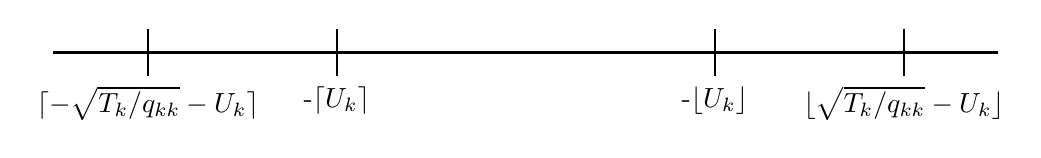
\begin{tikzpicture}[scale=6]
\draw[thick] (0.8,0.05)--(0.8,-0.05) node[anchor=north] {$\lfloor \sqrt{T_k/q_{kk}} - U_k \rfloor$};
\draw[thick] (-0.8,0.05)--(-0.8,-0.05) node[anchor=north]{$\lceil -\sqrt{T_k/q_{kk}} - U_k \rceil$};
\draw[thick] (0.4,0.05)--(0.4,-0.05) node[anchor=north] {-$\lfloor U_k \rfloor$};
\draw[thick] (-0.4,0.05)--(-0.4,-0.05) node[anchor=north]{-$\lceil U_k \rceil$};
\draw[thick] (-1,0)--(1,0);
\end{tikzpicture}
\end{center}

As stated above, 
\[\lceil -\sqrt{T_k/q_{kk}} - U_k \rceil= LB_k \leq y_k \leq UB_k = \lfloor \sqrt{T_k/q_{kk}} - U_k \rfloor.\]
In our old implementation for non-translated lattices, we set each $y_k = LB_k$ and increased each term until we reached the zero (centre) vector. Here since the centre vector is non-zero, we instead set each $y_k = -\lceil U_k \rceil$ and increase each $y_k$ successively until $y_k > \lfloor \sqrt{T_k/q_{kk}} - U_k \rfloor$. This is equivalent to the above computation and generates only half of the vectors, assuming symmetry. This symmetry can only be applied if the centre vector is defined over $\mathbb{Z}$, otherwise we must compute all vectors. To do (we can also break symmetry and compute all vectors in the $\mathbb{Z}$ case), we also set $y_k = \lceil U_k \rceil - 1$ and successively decrease this term until $y_k <\lceil -\sqrt{T_k/q_{kk}} - U_k \rceil$.

Of course, in this refinement, we want to avoid computing $\sqrt{T_k/q_{kk}}$, and so instead of verifying whether $y_k > \lfloor \sqrt{T_k/q_{kk}} - U_k \rfloor$ or $y_k <\lceil -\sqrt{T_k/q_{kk}} - U_k \rceil$, we compute $q_{kk}(y_k + U_k)^2$ in each case and verify whether
\[q_{kk}(y_k + U_k)^2 \leq C - \sum_{i = k+1}^m q_{ii}(y_i + U_i)^2\]
holds. In the first round, if this does not hold and if $y_k < -\lfloor U_k \rfloor$, we continue to iterate $y_k = y_k + 1$, otherwise we simply iterate $y_k = y_k + 1$. Once this equivalence does not hold and $y_k \geq -\lfloor U_k \rfloor$, we stop this loop. We then reset $y_k = \lceil U_k \rceil - 1$ and search in the other direction, by successively subtracting $1$ if 
\[q_{kk}(y_k + U_k)^2 \leq C - \sum_{i = k+1}^m q_{ii}(y_i + U_i)^2\]
holds. We stop searching in this direction only once this equivalence does not hold.  

%---------------------------------------------------------------------------------------------------------------------------------------------%

\subsection{Preliminaries: Elliptic Curves}

Let $K$ be a field. An \textit{elliptic curve} $E$ over $K$ is a nonsingular curve of the form 
\begin{equation} \label{elliptic}
E: y^2 + a_1xy + a_3y = x^3 + a_2x^2 + a_4x + a_6
\end{equation}
with $a_i \in K$, having a specified base point, $\mathcal{O}\in E$. An equation of the form (\ref{elliptic}) is called a \textit{Weierstrass equation}. For an elliptic curve $E$ over $K$, this equation is unique up to a coordinate transformation of the form
\[x = u^2x' + r, \quad\quad y = u^3y' + su^2x' + t, \]
with $r,s,t,u \in K, u\neq 0$. 
Writing 
\[b_2 = a_1^2 + 4a_2, \quad b_4 = a_1a_3 + 2a_4, \quad b_6 = a_3^2 + 4a_6,\]
\[b_8 = a_1^2a_6 + 4a_2a_6 - a_1a_3a_4 + a_2a_3^2 - a_4^2,\]
\[ c_4 = b_2^2 - 24b_4, \quad \text{ and } \quad c_6 = -b_2^3 + 36b_2b_4 + 9b_2b_4b_6,\]
if $\text{char}(K) \neq 2,3$, we can make several linear changes of variables so that, using these values, our elliptic curve has equation
\begin{equation} \label{curve}
E: y^2 = x^3 - 27c_4x - 54c_6.
\end{equation}
Associated to this curve are the quantities 
\[\Delta = -b_2^2b_8 - 8b_4^3 - 27b_6^2 + 9b_2b_4b_6 \quad \text{ and } \quad j = c_4^3/\Delta,\]
where $\Delta$ is called the \textit{discriminant} of the Weierstrass equation, and the quantity $j$ is called the \textit{j-invariant} of the elliptic curve. The condition of being nonsingular is equivalent to $\Delta$ being non-zero. Additionally, one may show that two elliptic curves are isomorphic over $\bar{K}$, the algebraic closure of $K$, if and only if they both have the same $j$-invariant.

When $K = \mathbb{Q}$, we can choose the Weierstrass model (\ref{elliptic}) with the $a_i \in \mathbb{Z}$ and the $p$-order of $\Delta$ minimal for each prime $p$. Supposing (\ref{elliptic}) is such a global minimal model for an elliptic curve $E$ over $\mathbb{Q}$, reducing the coefficients modulo a prime $p$, we obtain a (possibly singular) curve over $\mathbb{F}_p$, namely
\begin{equation}
\tilde{E}: y^2 + \tilde{a_1}xy + \tilde{a_3}y = x^3 + \tilde{a_2}x^2 + \tilde{a_4}x + \tilde{a_6},
\end{equation}
with $\tilde{a_i} \in \mathbb{F}_p$. This ``reduced" curve $\tilde{E}/\mathbb{F}_p$ is called the \textit{reduction of $E$ modulo} $p$. It is nonsingular provided that $\Delta \not \equiv 0 \mod{p}$, in which case it is an elliptic curve defined over $\mathbb{F}_p$. The curve $E$ is said to have \textit{good reduction} modulo $p$ if $\tilde{E}/\mathbb{F}_p$ is nonsingular, otherwise, we say $E$ has \textit{bad reduction} modulo $p$. 

The bad reduction of $E$ is measured by the \textit{conductor} of $E$, 
\[N = \prod_{p \text{ prime }}p^{f_p}, \]
where $f_p \neq 0$ if $p \nmid \Delta$ (so $f_p = 0$ for all but finitely many primes $p$), while $f_p = 1$ if the singularity is a node, and $f_p \geq 2$ if the singularity is a cusp. The $f_p$, hence the conductor, are invariant under isogeny. Hence, roughly speaking, the conductor $N$ is the product of primes at which $E$ has bad reduction raised to small powers, while the discriminant $\Delta$ is a product of the same primes, but they may sometimes appear to large powers.

%-----------------------------------------------------------------------------------------------------------------------------------------------
\subsection{Preliminaries: Cubic Forms}

Let $a,b,c$ and $d$ be integers, and consider the binary cubic form
\[F(x,y) = ax^3 + bx^2y + cxy^2 + dy^3.\]
Two such forms $F_1$ and $F_2$ are called \textit{equivalent} if they are equivalent under the $GL_{2}(\mathbb{Z})$-action. That is, if there exist integers $a_1, a_2, a_3$, and $a_4$ such that 
\[F_1(a_1x + a_2y, a_3x + a_4y) = F_2(x,y)\]
for all $x,y$, where $a_1a_4 - a_2a_3 = \pm 1$. In this case, we write $F_1 \sim F_2$. The \textit{discriminant} $D_F$ of such a form is given by 
\[D_F = -27a^2d^2 + b^2c^2 + 18abcd - 4ac^3 - 4b^3d = a^4 \prod_{i < j} (\alpha_i - \alpha_j)^2\]
where $\alpha_1, \alpha_2$ and $\alpha_3$ are the roots of the polynomial $F(x,1)$. We observe that if $F_1 \sim F_2$, then $D_{F_1} = D_{F_2}$. 

Associated to $F$ is the Hessian $H_F(x,y)$, given by
\begin{align*}
H_F(x,y) & = -\frac{1}{4}\left( \frac{\partial^2F}{\partial x^2} \frac{\partial^2F}{\partial y^2} - \left(\frac{\partial^2F}{\partial x \partial y}\right)^2\right)\\
& = (b^2 - 3ac)x^2 + (bc - 9ad)xy + (c^2 - 3bd)y^2,
\end{align*}
and the Jacobian determinant of $F$ and $H$, a cubic form $G_F(x,y)$ defined via 
\begin{align*}
G_F(x,y) &= \frac{\partial F}{\partial x} \frac{\partial H}{\partial y} - \frac{\partial F}{\partial y} \frac{\partial H}{\partial x} \\
& =  (-27a^2d + 9abc -2b^3)x^3 + (-3b^2c - 27abd + 18ac^2)x^2y +  \\
& \quad \quad + (3bc^2 - 18b^2d + 27acd)xy^2 + (-9bcd + 2c^3 + 27ad^2)y^3.
\end{align*}


%---------------------------------------------------------------------------------------------------------------------------------------------%
%---------------------------------------------------------------------------------------------------------------------------------------------%

\section{Goormaghtigh paper}
%--------------------------------------------------------------
\section{Rational approximations} \label{proof}
%--------------------------------------------------------------
%
%In what follows, we will always assume that $x, y, m$ and $n$ are integers satisfying (\ref{eq-main}) with (\ref{condition}), and write
%\begin{equation} \label{m0n0}
% m-1 = d m_0 \; \; \mbox{ and } \; \; n-1 = d n_0.
% \end{equation}
% We note, for future use, that  an appeal to Th\'eor\`eme II of Karanicoloff \cite{Ka} (which, in our notation, states that the only solution to (\ref{eq-main}) with $n_0=1$ and $m_0=2$ in (\ref{m0n0}) is given by $(x,y,m,n) = (2,5,5,3)$) allows us to suppose that either $(x,y,m,n) = (2,5,5,3)$, or that  $m_0 \geq 3$ and $n_0 \geq 1$.
%
%Our starting point, as in, for example, \cite{BuSh} and \cite{NeSh}, is the observation that the existence of a solution to (\ref{eq-main}) with (\ref{condition}) implies a number of unusually good rational approximations to certain irrational algebraic numbers. One such approximation arises from rewriting (\ref{eq-main}) as 
%$$
%x \, \frac{x^{d m_0}}{x-1} - y \, \frac{y^{d n_0}}{y-1} = \frac{1}{x-1} - \frac{1}{y-1},
%$$
%whereby
%\begin{equation} \label{good}
%\left| \sqrt[d]{\frac{y(x-1)}{x(y-1)}} - \frac{x^{m_0}}{y^{n_0}} \right| < \frac{1}{y^{d n_0}}.
%\end{equation}
%The latter inequality was used, in conjunction with lower bounds for linear forms in logarithms (in \cite{NeSh}) and with machinery based upon Pad\'e approximation to binomial functions (in \cite{BuSh}), to derive a number of strong restrictions upon $x, y$ and $d$ satisfying equation (\ref{eq-main}).
%
%Our argument will be somewhat different, as we consider instead a rational approximation to 
%$\sqrt[d]{(x-1)/x}$ that is, on the surface, much less impressive than that to $\sqrt[d]{\frac{y(x-1)}{x(y-1)}}$ afforded by (\ref{good}). The key additional idea is that we are able to take advantage of the arithmetic structure of our approximations  to obtain very strong lower bounds for how well they can approximate $\sqrt[d]{(x-1)/x}$. This argument has its genesis in work of Beukers \cite{Beu1}, \cite{Beu2}.
%
%For the remainder of this section, we will always assume that $x \geq 40$. From
% $$
% \frac{y^n-1}{y-1} = y^{dn_0} \left( 1 + \frac{1}{y} +  \cdots + \frac{1}{y^{dn_0}} \right) \mbox{ and }  \frac{x^m-1}{x-1} = x^{dm_0} \left( 1 + \frac{1}{x} + \cdots + \frac{1}{x^{dm_0}} \right) ,
% $$
% we thus have
% $$
%y^{dn_0}  <  \frac{y^n-1}{y-1} =  \frac{x^m-1}{x-1}  < \frac{x}{x-1} \,   x^{dm_0}
%$$
%and
%$$
%\frac{y}{y-1} \, x^{dm_0} \leq \frac{x+1}{x}  \, x^{dm_0} <  \frac{x^m-1}{x-1}  =  \frac{y^n-1}{y-1} 
%< \frac{y}{y-1} \, y^{dn_0},
%$$
%so that 
%\begin{equation} \label{goop}
%x^{m_0} < y^{n_0} <\left( \frac{x}{x-1} \right)^{1/d} \, x^{m_0} \leq \sqrt{40/39} \, x^{m_0} < 1.013 \, x^{m_0}.
%\end{equation}
%
%
%We will rewrite  (\ref{eq-main})
% as 
% $$
% x^{d m_0} -  \frac{(x-1)}{x} \;   \sum_{j=0}^{dn_0} y^j = \frac{1}{x}.
% $$
% From this equation, we will show that $\sqrt[d]{(x-1)/x}$ is well approximated by a rational number whose numerator is divisible by $x^{m_0}$.
% 
%If we define, as in Nesterenko and Shorey \cite{NeSh},  $A_k (d)$ via
%% $$
%% \left( 1 + \frac{1}{X} + \cdots + \frac{1}{X^{\mu-1}} \right)^{1/d} = \sum_{k=0}^\infty \frac{A_k (\mu,d)}{ X^{k}}
%% $$
%% and
% $$
%  \left( 1 - \frac{1}{X} \right)^{-1/d} = \sum_{k=0}^\infty A_k (d) \, X^{-k} = \sum_{k=0}^\infty
%  \frac{d^{-1} ( d^{-1}+1) \cdots (d^{-1} + k-1)}{k!} \, X^{-k},
% $$
% then we can write 
% $$
% \sum_{j=0}^{dn_0} y^j = \left( \sum_{k = 0}^{n_0} A_k (d) y^{n_0-k} \right)^d + \sum_{j=0}^{(d-1)n_0-1} B_j(d) y^j.
% $$
%Here, the $B_j$ are positive, monotone increasing in $j$, and satisfy
% $$
% B_{(d-1)n_0-1} (d) = \frac{n}{n_0+1} A_{n_0} (d),
% $$
% while, for the $A_k(d)$, we have the inequalities
% $$
% \frac{d+1}{k d^2} \leq A_k (d) \leq  \frac{d+1}{2 d^2},
% $$
%valid  provided $k \geq 2$ (see displayed equation (14) of \cite{NeSh}). 
%%Note that
%% $$
%% A_{k+1} (d) = \frac{d^{-1}+k}{1+k} \, A_k (d).
% %$$
% 
% We thus have
%\begin{equation} \label{careful}
% x^{d m_0} -  \frac{(x-1)}{x} \; \left( \sum_{k = 0}^{n_0} A_k (d) y^{n_0-k} \right)^d = \frac{1}{x} + \frac{x-1}{x} \, \sum_{j=0}^{(d-1)n_0-1} B_j(d) y^j
% \end{equation}
% and so
% \begin{equation} \label{careful-upper}
% 0 <  x^{d m_0} -  \frac{(x-1)}{x} \; \left( \sum_{k = 0}^{n_0} A_k (d) y^{n_0-k} \right)^d <  \frac{(dn_0+1)(d+1)}{2 (n_0+1) d^2} \, \frac{y}{y-1} \, y^{(d-1) n_0-1}.
% \end{equation}
% Since
% $$
% \frac{(dn_0+1)(d+1)}{2 (n_0+1) d^2} < \frac{d+1}{2d} \leq \frac{3}{4},
% $$
%from the fact that $n_0 \geq 1$ and $d \geq 2$, and since $y > x \geq 40$, we may conclude that
%  \begin{equation} \label{careful-upper2}
% 0 <  x^{d m_0} -  \frac{(x-1)}{x} \; \left( \sum_{k = 0}^{n_0} A_k (d) y^{n_0-k} \right)^d < 0.769 \, y^{(d-1) n_0-1}.
% \end{equation}
% Applying the Mean Value Theorem,
%  \begin{equation} \label{careful-upper3}
% 0 <   x^{m_0} -  \sqrt[d]{\frac{x-1}{x}} \, \sum_{k = 0}^{n_0} A_k (d) y^{n_0-k}  <  0.769 \,  \frac{y^{(d-1) n_0-1}}{d Y^{d-1}},
%  \end{equation}
%  where $Y$ lies in the interval
%  $$
%  \left( \sqrt[d]{\frac{x-1}{x}} \, \sum_{k = 0}^{n_0} A_k (d) y^{n_0-k}, x^{m_0} \right).
%  $$
% We thus have
% $$
% Y^{d-1} >  \left( \frac{x-1}{x} \right)^{(d-1)/d} \, y^{(d-1) n_0}
% $$
% and so, from (\ref{careful-upper3}) and the fact that $d \geq 2$ and $x \geq 40$, 
%   \begin{equation} \label{careful-upper4}
% 0 <   x^{m_0} -  \sqrt[d]{\frac{x-1}{x}} \, \sum_{k = 0}^{n_0} A_k (d) y^{n_0-k}  <  \frac{0.779}{d y}.
%  \end{equation}
%  
%Let us define
% $$
% C(k,d) = d^k \prod_{p \mid d} p^{\mbox{ord}_p (k!)},
% $$
% where by $\mbox{ord}_p(z)$ we mean the largest power of $p$ that divides a nonzero integer $z$. Here,
% $k$  and $d$ positive integers with $d \geq 2$. Then we have
%$$
%C(k,d) =  d^k \prod_{p \mid d} p^{\left[ \frac{k}{p} \right] + \left[ \frac{k}{p^2} \right] + \cdots}
%$$
%and hence it follows that
%\begin{equation} \label{C-upper}
%C(k,d) < \left( d \,  \prod_{p \mid d} p^{1/(p-1)} \right)^k.
%\end{equation}
%Further (see displayed equation (18) of Nesterenko and Shorey \cite{NeSh}), and critically for our purposes, $C(k,d) A_k (d)$ is an integer. Multiplying equation (\ref{careful}) by $C(n_0,d)$ and setting 
%\begin{equation} \label{P-Q-def}
% P = C(n_0,d) \,  x^{m_0} \; \; \mbox{ and } \; \; Q = C(n_0,d) \,  \sum_{k = 0}^{n_0} A_k (d) y^{n_0-k},
%\end{equation}
% then $P$ and $Q$ are integers  and, defining
%\begin{equation} \label{ep-def}
%\epsilon = P - \sqrt[d]{\frac{x-1}{x}} Q,
%\end{equation}
% we thus have, from (\ref{careful-upper4}), that the following result holds.
% \begin{prop} \label{upper-ep}
% Suppose that $(x,y,m,n)$ is a solution in integers to equation (\ref{eq-main}), with (\ref{condition}) and $x \geq 40$. If we define $\epsilon$ via (\ref{ep-def}),  then
%\begin{equation} \label{start}
%0 < \epsilon < \frac{0.779 \, C(n_0,d)}{dy}.
%\end{equation}
% \end{prop}
% 
%Our next goal will be to construct a second linear form $\delta$, in $1$ and $\sqrt[d]{(x-1)/x}$, with the property that a particular linear combination of $\epsilon$ and $\delta$ is a (relatively large) nonzero integer, a fact we will use to derive a lower bound on $\epsilon$. This argument, which will employ off-diagonal Pad\'e approximants to the binomial function $\sqrt[d]{1+z}$, follows work of Beukers \cite{Beu1}, \cite{Beu2}.
%
%To apply Proposition \ref{upper-ep} and for our future arguments, we will have use of bounds upon the quantity $C(k,d)$. 
% \begin{prop} \label{Cee}
%If $k$ is a positive integer, then
%$$
%2^k \leq C(k,2) < 4^k
%$$
%and
%$$
%d^k \leq C(k,d) < (2 d \log d)^k,
%$$
%for $d > 2$.
%\end{prop}
%We will postpone the proof of this result until Section \ref{Cee-proof}; the upper bound here for large $d$ may be sharpened somewhat, but this is unimportant for our purposes.
%
%%---------------------------------------------------------
%\section{Pad\'e approximants} \label{Pade}
%%--------------------------------------------------------
%
%
%In this section, we will define Pad\'e approximants to $(1+z)^{1/d}$, for $d \geq 2$.
%Suppose that $m_1$ and $m_2$ are nonnegative integers, and set
%$$
%I_{m_1,m_2}(z) = \frac{1}{2 \pi i} \, \int_{\gamma} ~
%\frac{(1+zv)^{m_2}(1+zv)^{1/d}}{v^{m_1+1} (1-v)^{m_2+1}} \, dv,
%$$
%where $\gamma$ is a closed, counter-clockwise contour, containing $v=0$ and $v=1$. Applying Cauchy's residue theorem, we may write $I_{m_1,m_2}(z)$ as $R_0+R_1$, where
%$$
%R_i = \mbox{Res}_{v=i} \left( \frac{(1+zv)^{m_2}(1+zv)^{1/d}}{v^{m_1+1} (1-v)^{m_2+1}} \right). 
%$$
%Now
%$$
%R_0=
%\frac{1}{m_1!} \, \lim_{v \rightarrow 0} \frac{d^{m_1}}{dv^{m_1}} \, \frac{(1+zv)^{m_2}(1+zv)^{1/d}}{(1-v)^{m_2+1}} = P_{m_1,m_2} (z) 
%$$
%and
%$$
%R_1=
%\frac{1}{m_2!} \, \lim_{v \rightarrow 1} \frac{d^{m_2}}{dv^{m_2}} \, \frac{(1+zv)^{m_2}(1+zv)^{1/d}}{v^{m_1+1}} =  - Q_{m_1,m_2} (z) \, (1+z)^{1/d},
%$$
%where
%\begin{equation}  
%P_{m_1,m_2} (z) = \sum_{k=0}^{m_1} \binom{m_2 + 1/d}{k} \binom{m_1+m_2-k}{m_2} z^k
%\end{equation}
%and
%\begin{equation} \label{queu}
%Q_{m_1,m_2} (z) = \sum_{k=0}^{m_2} \binom{m_1 - 1/d}{k} \binom{m_1+m_2-k}{m_1} z^k.
%\end{equation}
%Note that there are typographical errors in the analogous statement given in displayed equation (2.3) of \cite{BaBe}.
%We take $z=-1/x$. Arguing as in the proof of Lemma 4.1 of \cite{BaBe}, we find that
%\begin{equation} \label{del0}
%|I_{m_1,m_2}(-1/x)| = \frac{\sin (\pi/d)}{\pi \,  x^{m_1+m_2+1}} \;  \int^{1}_{0} ~
%\frac{v^{m_2+1/d} (1-v)^{m_1-1/d} dv}{(1-(1-v)/x)^{m_2+1}}.
%\end{equation}
%Upon multiplying the identity
%$$
%P_{m_1, m_2}(-1/x)-Q_{m_1, m_2}(-1/x)   \sqrt[d]{\frac{x-1}{x}} =I_{m_1,m_2}(-1/x) 
%$$
%through by $x^{m_2} C(m_2,d)$,
%and setting
%$$
%\delta = C_0 P_1 -  \sqrt[d]{\frac{x-1}{x}} \; Q_1,
%$$
%where we write $m_0=m_2-m_1$,
%$$
%C_0 = x^{m_0} C(m_2,d)/C(m_1,d), \; \; P_1 = x^{m_1} C(m_1,d) P_{m_1,m_2}(-1/x)
%$$
%and
%\begin{equation} \label{Q1-def}
%Q_1=x^{m_2} C(m_2,d) Q_{m_1,m_2}(-1/x),
%\end{equation}
%it follows, from Lemma 3.1 of Chudnovsky \cite{Chud},
%that $C_0, P_1$ and $Q_1$ are integers. Further, from (\ref{del0}), 
%\begin{equation} \label{del}
%|\delta| = \frac{\sin (\pi/d) \, C(m_2,d)}{\pi \,  x^{m_1+1}} \;  \int^{1}_{0} ~
%\frac{v^{m_2+1/d} (1-v)^{m_1-1/d} dv}{(1-(1-v)/x)^{m_2+1}}.
%\end{equation}
%
%%Then (see e.g. ), we have that
%%\begin{equation} \label{aye}
%% P_{m_1,m_2} (z) - \left( 1+z \right)^{1/d} \; Q_{m_1,m_2} (z) = z^{m_1+m_2+1} \, E_{m_1,m_2} (z),
%%\end{equation}
%%where 
%%\begin{equation} \label{frump}
%%E_{m_1,m_2} (z) =   \frac{(-1)^{m_2} \, \Gamma (m_2+(d+1)/d)}{\Gamma(-m_1+1/d) \Gamma(m_1+m_2+2)}  F(m_1 + (d-1)/d,m_2+1, m_1+m_2+2,-z),
%%\end{equation}
%%for $F$ the hypergeometric function given by
%%$$
%%F(a,b,c,-z) = 1 - \frac{a \cdot b}{1 \cdot c} z + \frac{a \cdot (a+1) \cdot b \cdot (b+1)}{1 \cdot 2 \cdot c \cdot (c+1)} z^2 - \cdots.
%%$$
%
%Recall that $P$ and $Q$ are defined as in (\ref{P-Q-def}). Here and henceforth, we will assume that 
%\begin{equation} \label{sturdy}
%m_2-m_1=m_0. 
%\end{equation}
%We have
%\begin{lem} \label{pumpkin}
%If  $m_1$ and $m_2$ are nonnegative integers satisfying (\ref{sturdy}),  then it follows that $PQ_1 \neq C_0 P_1 Q$.
%\end{lem}
%
%\begin{proof}
%Let $p$ be a prime with $p \mid d$. 
%Then
%$$
%\mbox{ord}_p (P) = n_0 \, \mbox{ord}_p (d)  + \mbox{ord}_p (n_0!) + m_0 \, \mbox{ord}_p (x),
%$$
%$$
%\mbox{ord}_p (P_1) = \mbox{ord}_p (Q_1) = \mbox{ord}_p (Q) = 0
%$$
%and
%$$
%\mbox{ord}_p (C_0) = m_0 \, \mbox{ord}_p (d)  + \mbox{ord}_p (m_2!)  - \mbox{ord}_p (m_1!) + m_0 \, \mbox{ord}_p (x).
%$$
%Since $m_2 - m_1 = m_0 > n_0$, 
%we have
%$$
%\mbox{ord}_p \left( \frac{C_0P_1 Q}{P Q_1} \right) = (m_0-n_0)  \, \mbox{ord}_p (d)  + \mbox{ord}_p \left( \frac{m_2!}{m_1! n_0!} \right) > 0
%$$
%so that 
%$$
%\mbox{ord}_p (P Q_1 - C_0 P_1 Q) = \mbox{ord}_p (P Q_1) = n_0 \, \mbox{ord}_p (d)  + \mbox{ord}_p (n_0!) + m_0 \, \mbox{ord}_p (x)
%$$
%and, in particular, $P Q_1 - C_0 P_1 Q \neq 0$.
%
%\end{proof}
%
%%Appealing twice to  (\ref{aye}) and  (\ref{frump}) with, in the second instance,  $m_2$ replaced by $m_2+1$, and eliminating $(1+z)^{1/q}$,  we find that $P_{m_1,m_2+1}(z)Q_{m_1,m_2}(z)-P_{m_1,m_2}(z)Q_{m_1,m_2+1}(z)$ is a polynomial of degree $m_1+m_2+1$ with a zero at $z=0$ of order $m_1+m_2+1$ (and hence monomial). It follows that we may write
%%\begin{equation} \label{zero}
%%P_{m_1,m_2+1}(z)Q_{m_1,m_2}(z)-P_{m_1,m_2}(z)Q_{m_1,m_2+1}(z) = c z^{m_1+m_2+1},
%%\end{equation}
%%with, a short calculation reveals, $c \neq 0$.
%
%It follows from Lemma \ref{pumpkin}
%and its proof  that $P Q_1 - C_0 P_1 Q$ is a nonzero integer multiple of 
%$C(n_0,d) \, x^{m_0}$, so that, from the definitions of $\epsilon$ and $\delta$, 
%\begin{equation} \label{key}
%|\epsilon Q_1 - \delta Q| = |P Q_1 - C_0 P_1 Q| \geq  C(n_0,d) \, x^{m_0}.
%\end{equation}
%
%Now 
%$$
%Q = C(n_0,d) \,  \sum_{k = 0}^{n_0} A_k (d) y^{n_0-k} < \frac{y}{y-1} \, C(n_0,d) \, y^{n_0} \leq 1.025 \, C(n_0,d) \, y^{n_0},
%$$
%since $y > x \geq 40$, and hence,
%from (\ref{goop}), 
%\begin{equation} \label{Q-upper}
%Q < 1.039  \, C(n_0,d) \, x^{m_0}.
%\end{equation}
%
%Combining (\ref{goop}), (\ref{start}), (\ref{key}) and (\ref{Q-upper}), we thus have
% \begin{prop} \label{upper-cool}
% Suppose that $(x,y,m,n)$ is a solution in integers to equation (\ref{eq-main}), with (\ref{condition}) and $x \geq 40$. If $m_0, n_0$ and $d$ are defined as in (\ref{m0n0}), and $m_1$ and $m_2$ are nonnegative integers satisfying (\ref{sturdy}), then for $Q_1$ and $|\delta|$ as given  in (\ref{Q1-def}) and (\ref{del}), we may conclude that
% \begin{equation} \label{imp}
%  |Q_1| > 1.28 \, d \, (1-1.039 |\delta|) \, x^{m_0+m_0/n_0}.
%\end{equation}
% \end{prop}
%
%In the other direction, we will deduce two upper bounds upon $|Q_1|$; we will use one or the other depending on whether or not $m_1$ is ``large'', relative to $x$. The first result is valid for all choices of $x$.
%\begin{prop} \label{shazam2}
%If $m_1, m_2$ and $x$ are integers with $m_2 > m_1 \geq 1$ and $x \geq 2$, define $\alpha = m_2/m_1$ and $|\delta|$ as in (\ref{del}).
%Then
%\begin{equation} \label{munchkin}
%|Q_1| < \sqrt[d]{\frac{x}{x-1}} \; \left( \frac{(\alpha+1)^2}{\alpha} \, (e \, (\alpha + 1))^{m_1}  \, x^{m_2} \, C(m_2,d)
%+ |\delta| \right).
%\end{equation}
%\end{prop}
%
%
%If $x \geq m_1$, we will have use of the following slightly sharper bound.
% \begin{prop} \label{shazam}
%If $m_1$ and $m_2$ are integers with $m_2 > m_1 \geq 0$ and $x \geq \frac{m_1m_2}{m_1+m_2}$, then
%$$
%|Q_1| < \frac{x}{x-1} \, \binom{m_1+m_2}{m_1}  \, C(m_2,d) \, x^{m_2}.
%$$
%\end{prop}
%
%\begin{proof}[Proof of Proposition \ref{shazam2}]
%Let us write $\alpha = m_2/m_1>1$
%and define
%\begin{equation} \label{arrr}
%r (\alpha,  u) =
%\frac{1}{2u} \left( (\alpha + 1) - (\alpha - 1) u - \sqrt{\left((\alpha + 1) - (\alpha - 1) u \right)^2 - 4 u} \right),
%\end{equation}
%and
%\begin{equation} \label{emm}
%M(\alpha,x) =  \frac{(1-r(\alpha,1/x)/x)^{\alpha}}{(1-r(\alpha,1/x))^{\alpha} r(\alpha,1/x)}.
%\end{equation}
%
%Via the Mean Value Theorem, 
%\begin{equation} \label{upper-al}
% \frac{1}{\alpha +1}  < r(\alpha,1/x) < \frac{x}{(x-1)(\alpha +1)}
%\end{equation}
%and so, from calculus,
%\begin{equation} \label{upper-emm}
%M(\alpha,x) < \left( \frac{(x-1) \, (\alpha+1)-1}{(x-1) (\alpha +1)-x} \right)^\alpha \cdot (\alpha+1) < e \, (\alpha +1)
%\end{equation}
%and
%\begin{equation} \label{M-lower}
%M(\alpha,x) > \left( 1 + \frac{x-1}{x \alpha} \right)^\alpha \, \left( \frac{x-1}{x} \right) \; (\alpha+1).
%\end{equation}
%
%Arguing as in the proof of Lemma 3.1 of \cite{BaBe}, we find that 
%$$
%|C_0 P_1| \leq \frac{\left( 1-r(\alpha,1/x)/x \right)^{1/d}}{r(\alpha, 1/x) (1 - r(\alpha,1/x))} \, M(\alpha,x)^{m_1} \, x^{m_2} \, C(m_2,d),
%$$
%whereby inequalities (\ref{upper-al}) and  (\ref{upper-emm}) imply that
%$$
%|C_0 P_1| < \frac{(\alpha+1)^2}{\alpha} \, (e \, (\alpha + 1))^{m_1}  \, x^{m_2} \, C(m_2,d).
%$$
%Since $C_0 P_1 = \sqrt[d]{\frac{x-1}{x}} \; Q_1 + \delta$, we conclude as desired.
%\end{proof}
%
%\begin{proof}[Proof of Proposition \ref{shazam}]
%To bound $Q_1$ from above, we begin by noting that
%\begin{equation} \label{naslund}
%x^{m_2} \left| Q_{m_1,m_2} (-1/x) \right| = \left| \sum_{k=0}^{m_2} \binom{m_1 - 1/d}{k} \binom{m_1+m_2-k}{m_1} (-1)^k x^{m_2-k} \right|.
%\end{equation}
%Defining
%$$
%f (k) = \binom{m_1 - 1/d}{k} \binom{m_1+m_2-k}{m_1},
%$$
%it follows that, for $0 \leq k \leq m_2-1$,
%$$
%f (k+1)/f(k) = \frac{(m_1 -1/d-k)(m_2-k)}{(k+1)(m_1+m_2-k)}.
%$$
%If $k \leq m_1-1$, we thus have that
%\begin{equation} \label{bound1}
%0 < f (k+1)/f(k) < \frac{(m_1 -k)(m_2-k)}{(k+1)(m_1+m_2-k)} \leq \frac{m_1m_2}{m_1+m_2}.
%\end{equation}
%If instead $k \geq m_1$, 
%\begin{equation} \label{bound2}
%\frac{(m_1 -k-1)(m_2-k)}{(k+1)(m_1+m_2-k)}  < f (k+1)/f(k) < 0.
%\end{equation}
%It follows via calculus, in this case, that
%$$
%|f(k+1)/f(k)| < \frac{(m_2-m_1+1)^2}{(m_2+m_1+1)^2}.
%$$
%We thus have that $x^{m_2} \left| Q_{m_1,m_2} (-1/x) \right|$ is bounded above by
%$$
% \binom{m_1+m_2}{m_1}  x^{m_2} +  \left| \binom{m_1 - 1/d}{m_1} \right| \binom{m_2}{m_1}  \sum_{k=m_1+1}^{m_2}  x^{m_2-k}
%$$
%which implies the desired result. 
%\end{proof}
%
%
%%------------------------------------------------------
%\section{Proof of Theorem \ref{main-thm} } \label{sec-main-thm}
%%------------------------------------------------------
%
%To prove Theorem \ref{main-thm}, we will work with Pad\'e approximants to $(1+z)^{1/d}$, as in Section \ref{Pade},  of degrees $m_1$ and $m_2$ where we choose
%\begin{equation} \label{choice}
%m_1 = \left[ \frac{m_0}{2 n_0} \right] \; \; \mbox{ and } \; \; m_2 = m_0 + \left[ \frac{m_0}{2 n_0} \right],
%\end{equation}
%for $m_0, n_0$ and $d$ as given in (\ref{m0n0}). Here $[x]$ denotes the greatest integer less than or equal to $x$.
%Let us assume further that $x \geq (3d)^{4n/d} \geq 6^6$. 
%We will make somewhat different choices later, when we prove Theorem \ref{main-thm2}. 
%
%Our strategy will be as follows. We begin by showing that 
% $\delta$ as given in (\ref{del}) satisfies $|\delta| < \frac{1}{1.039}$, so that the lower bound upon $|Q_1|$ in Proposition \ref{upper-cool} is nontrivial. From there, we will appeal to Proposition \ref{shazam2}  to contradict Proposition \ref{upper-cool}.
% 
%%----------------------------------
%\subsection{Bounding $\delta$}
%%----------------------------------
%
%From the aforementioned Th\'eor\`eme II of Karanicoloff \cite{Ka}, we may suppose that $m_0 \geq 3$ and hence, arguing crudely, since $m_2 \geq m_0 \geq 3$ and $m_1 \geq 0$, we have
%$$
% \int^{1}_{0} ~
%\frac{v^{m_2+1/d} (1-v)^{m_1-1/d} dv}{(1-(1-v)/x)^{m_2+1}} < 1
%$$
%and hence, from (\ref{del}), 
%\begin{equation} \label{frog}
%|\delta| < \frac{\sin (\pi/d) \, C(m_2,d)}{\pi \,  x^{m_1+1}} \leq \frac{C(m_2,d)}{\pi \,  x^{m_1+1}}.
%\end{equation}
% 
%From (\ref{choice}),  $m_1+1 > \frac{m_0}{2 n_0}$ and so, the  assumption that $x \geq (3d)^{4n/d}$ yields the inequality 
%$$
%x^{m_1+1} >  (3d)^{2 m_0}. 
%$$
%Applying Proposition \ref{Cee}, if $d=2$, it follows from $m_1 \leq \frac{m_0}{2n_0}$ that 
%$$
%|\delta| <  \frac{1}{\pi} \, 4^{m_1} \, 3^{-2m_0} \leq \frac{8}{729 \pi} < 0.01,
%$$
%since $m_0 \geq 3$ and $n_0 \geq 1$.
%Similarly, if $d \geq 3$, 
%$$
%|\delta| <  \frac{(2 d \log d)^{m_0+m_1}}{(3d)^{2m_0}} \leq \frac{(2 d \log d)^{m_0+\frac{m_0}{2n_0}}}{(3d)^{2m_0}}
%= \left( \frac{(2 d \log d)^{1+\frac{1}{2n_0}}}{9d^{2}} \right)^{m_0} < 0.01,
%$$
%again from $m_0 \geq 3$ and $n_0 \geq 1$.
%Appealing to Proposition \ref{upper-cool}, we thus have, in either case,
%\begin{equation} \label{moving}
% |Q_1| > 1.25 \, d \, x^{m_0+m_0/n_0}.
%\end{equation}
%
%
%%-------------------------------------------------------------
%\subsection{Applying Proposition \ref{shazam2}}
%%-------------------------------------------------------------
%
%We will next apply Proposition \ref{shazam2} to deduce an upper bound upon $|Q_1|$. To use this result, we must first separately treat the case when $m_1=0$. In this situation, 
%Proposition \ref{shazam} implies that
%$$
%|Q_1| < \frac{x}{x-1}   \, C(m_0,d) \, x^{m_0}.
%$$
%Inequality (\ref{moving}) and $x \geq (3d)^{4n/d} > (3d)^{4n_0}$ thus lead to the inequalities 
%$$
%C(m_0,d) > d \, x^{m_0/n_0} > (3d)^{4 m_0},
%$$
%contradicting Proposition \ref{Cee} in all cases.
%
%Assuming now that $m_1 \geq 1$, combining  Proposition \ref{shazam2} with (\ref{moving}), $d \geq 2$ and the fact that $\alpha = 1+m_0/m_1 \geq 3$, implies that
%$$
%x^{\frac{m_0}{n_0} - m_1} <  \alpha \, C(m_2,d) \, (e \, (\alpha+1))^{m_1}.
%$$
%Since $m_1 \leq m_0/2n_0$, $x \geq (3d)^{4n/d} > (3d)^{4n_0}$ and $\alpha = 1+m_0/m_1$, it follows that
%$$
%(3d)^{2m_0} < (1 + m_0/m_1) \,  C(m_0+m_1,d) \,   (e \, (2 + m_0/m_1))^{m_1}
%$$
%and so
%\begin{equation} \label{fish}
%9 d^2 < (1 + m_0/m_1)^{1/m_0}  \,  C(m_0+m_1,d)^{1/m_0} \,   (e \, (2 + m_0/m_1))^{m_1/m_0}.
%\end{equation}
%If $d=2$, Proposition \ref{Cee} yields
%\begin{equation} \label{fleece}
%36 < (1 + m_0/m_1)^{1/m_0}  \,  4^{1+m_1/m_0} \,   (e \, (2 + m_0/m_1))^{m_1/m_0},
%\end{equation}
%contradicting  the fact that $m_0 \geq \max \{ 3, 2m_1 \}$.
%
%If $d \geq 3$, (\ref{fish}) and Proposition \ref{Cee}  lead to the inequality
%$$
%9 d^2 < (1 + m_0/m_1)^{1/m_0}  \,  (2 d \log d)^{1+m_1/m_0} \,   (e \, (2 + m_0/m_1))^{m_1/m_0},
%$$
%whence
%\begin{equation} \label{bluff}
%2.744 < \frac{9 \sqrt{d}}{2 \sqrt{2} (\log d)^{3/2}} < (1 + m_0/m_1)^{1/m_0}  \,  (e \, (2 + m_0/m_1))^{m_1/m_0}.
%\end{equation}
%If $n_0 \geq 3$, then $m_0 \geq 6 m_1$ and hence 
%$$
%(1 + m_0/m_1)^{1/m_0}  \,  (e \, (2 + m_0/m_1))^{m_1/m_0} < 2.4,
%$$
%a contradiction, while, from the second inequality in (\ref{bluff}), we find that  $d \leq 1112$ or $d \leq 64$, if $n_0=1$ or $n_0=2$, respectively. 
%
%For these remaining values, we will argue somewhat more carefully. From (\ref{C-upper}) and (\ref{fish}), 
%\begin{equation} \label{flag}
%9 d^2 < (1 + m_0/m_1)^{1/m_0}  \,  \left( d \,  \prod_{p \mid d} p^{1/(p-1)} \right)^{1+m_1/m_0} \,   (e \, (2 + m_0/m_1))^{m_1/m_0}.
%\end{equation}
%If $n_0=2$ (so that $m_0 \geq 4 m_1$), we thus have
%$$
%d^{3/4} <  0.34 \, \left( \prod_{p \mid d} p^{1/(p-1)} \right)^{5/4},
%$$
%and hence, for $3 \leq d \leq 64$, a contradiction. Similarly, if $n_0=1$, we have from $m_0 \geq 3$ that either $(m_0,m_1)=(3,1)$ or $m_0 \geq 4$. In the first case,
%$$
%d^{2/3} <  0.43 \, \left( \prod_{p \mid d} p^{1/(p-1)} \right)^{4/3},
%$$
%contradicting the fact that $d \leq 1112$. If $m_0 \geq 4$ (so that $m_1 \geq 2$), then (\ref{flag}) implies the inequality
%$$
%d^{1/2} <  \frac{e^{1/2} \cdot 2 \cdot 3^{1/2m_1}}{9}  \, \left( \prod_{p \mid d} p^{1/(p-1)} \right)^{3/2}
%$$
%and hence, after a short computation and using that $d \le 1112$, either $d=6$, $m_0=2m_1$ and $m_1 \leq 15$, or $d=30$ and $(m_0,m_1)=(4,2)$.
%In this last case, 
%$$
%x^6 Q_{2,6} (-1/x) = \sum_{k=0}^{6} \binom{2 - 1/30}{k} \binom{8-k}{2} (-x)^{6-k}
%$$
%and so $x^6 Q_{2,6} (-1/x)$ is equal to 
%$$
%28 x^6-\frac{413}{10} x^5+ \frac{1711}{120} x^4+ \frac{1711}{16200} x^3+\frac{53041}{3240000} x^2+\frac{3235501}{972000000} x + \frac{294430591}{524880000000}
%< 28 x^6,
%$$
%since $x \geq 6^6$. 
%From $C(6,30)=52488000000$, we have that
%$$
%|Q_1| < 1.47 \cdot 10^{13} \, x^6.
%$$
%On the other hand,  (\ref{moving}) implies that $|Q_1| > 37.5 \cdot x^8$, so that $x < 6.3 \cdot 10^5$,
%contradicting $x \geq (3d)^{4n/d} > 90^{4}$.
%
%For $d=6$, $2 \leq m_1 \leq 15$ and $m_0=2m_1$, we argue in a similar fashion, explicitly computing $Q_{m_1,m_2} (z)$ and finding that
%$$
%|Q_1| < \kappa_{m_1} x^{3m_1},
%$$
%where
%$$
%\begin{array}{cc|cc|cc}
%m_1 & \kappa_{m_1} & m_1 & \kappa_{m_1}  &  m_1 & \kappa_{m_1} \\ \hline
%2 & 1.89 \cdot 10^8 & 7 & 1.35 \cdot 10^{32} & 12 & 1.60 \cdot 10^{57}  \\
%3 & 2.30 \cdot 10^{13} & 8 & 1.24 \cdot 10^{37} &  13 & 1.89 \cdot 10^{61} \\ 
%4 & 9.86 \cdot 10^{17} & 9 & 1.29 \cdot 10^{42} & 14 & 1.79 \cdot 10^{66}  \\ 
%5 & 1.09 \cdot 10^{22} & 10 & 6.02 \cdot 10^{46}  & 15 & 1.28 \cdot 10^{71} \\
%6 & 5.88 \cdot 10^{27} & 11 &  1.13 \cdot 10^{52} & &  \\
%\end{array}
%$$
%With (\ref{moving}), we thus have
%$$
%x^{m_1} <  \frac{2}{15} \, \kappa_{m_1},
%$$
%and so
%$$
%x < \left( \frac{2}{15} \, \kappa_{m_1} \right)^{1/m_1} < 5.5 \cdot 10^4,
%$$
%contradicting our assumption that $x \geq 18^{2n/3} \geq 18^{14/3} > 7.2 \cdot 10^5$. This completes the proof of Theorem \ref{main-thm}.
%
%
%%------------------------------------------------------
%\section{Proof of Theorem \ref{main-thm2} for $x$ of moderate size }  \label{sec-main-thm2}
%%------------------------------------------------------
%
%As can be observed from the proof of Theorem \ref{main-thm}, the upper bound $x <  (3d)^{4n/d}$ may, for fixed values of $n$ (and hence $d$), be improved with a somewhat more careful argument. By way of example, for small choices of $n$, we may derive bounds of the shape $x < x_0(n)$, provided we assume that $m \geq m_0 (n)$ for effectively computable $m_0$, where we have
%$$
%\begin{array}{cc|cc|cc|cc} \hline
%n & x_0(n) & n & x_0(n) & n & x_0(n) & n & x_0(n) \\ \hline
%3 & 38 & 5 & 676 & 7 & 11647 & 9 & 195712 \\
%4 & 80  & 6 & 230 & 8 & 492 & 10 &  72043. \\
%\end{array}
%$$
%To prove Theorem \ref{main-thm2}, we will begin by deducing slightly weaker versions of these bounds, for $n \in \{ 3, 4, 5 \}$, where the corresponding values $m_0$ are amenable to explicit computation. Our arguments will closely resemble those of the preceding section, with slightly different choices of $m_1$ and $m_2$, and with a certain amount of additional care. Note that, from Theorem \ref{main-thm}, we may assume that we are in one of the following cases
%\begin{enumerate}
%\item $n=3, \; d=2, \;  n_0=1, \; 2 \leq x \leq 46655$,
%\item $n=4, \; d=3, \; n_0=1, \; 2 \leq x \leq 122826$,
%\item $n=5, \; d=2, \; n_0=2, \; 2 \leq x \leq 60466175$,
%\item $n=5, \; d=4, \; n_0=1, \; 2 \leq x \leq 248831$.
%\end{enumerate}
%Initially, we will suppose that $x \geq 40$ and, in all cases, that $m_1$ and $m_2$ are nonnegative integers satisfying (\ref{sturdy}). We will always, in fact, choose $m_1$ positive. Again setting $m_2=\alpha m_1$, 
%via calculus, we may bound the integral $\int^{1}_{0} ~
%\frac{v^{m_2+1/d} (1-v)^{m_1-1/d} dv}{(1-(1-v)/x)^{m_2+1}}$ in (\ref{del}) by
%$$
%\left( \max_{v \in [0,1]} \frac{v^{(\alpha+1)/d}}{ \left( 1 - (1-v)/x \right)^{(\alpha+d)/d}} \right) 
%\; M(\alpha,x)^{1/d-m_1} < M(\alpha,x)^{1/d-m_1}.
%$$
%From (\ref{del}), it thus follows that
%\begin{equation} \label{del-upper}
%|\delta| < \frac{\sin (\pi/d) \, C(m_2,d)}{\pi \,  x^{m_1+1}} \;  M(\alpha,x)^{1/d-m_1}.
%\end{equation}
%
%
%%-------------------------------------------------------------------------------
%\subsection{Case (1) : $n=3, \; d=2, \;  n_0=1, \; x \geq 40$}
%%-------------------------------------------------------------------------------
%
%In this case, we will take
%$$
%m_1 = \Big\lceil \frac{2m_0}{7} \Big\rceil \; \; \mbox{ and } \; \; m_2 = m_0+  \Big\lceil \frac{2m_0}{7} \Big\rceil,
%$$
%where by $\lceil x \rceil$ we mean the least integer that is $\geq x$, so that $m_1 \geq 2 m_2/9$, i.e. $\alpha \leq 9/2$. 
%From (\ref{del-upper}) and   Proposition \ref{Cee}, 
%$$
%|\delta| < \frac{M(\alpha,x)^{1/2}}{\pi x} \; \left( \frac{4^{\alpha} }{x \, M(\alpha,x)} \right)^{m_1}.
%$$
%Appealing to (\ref{M-lower}), since $x \geq 40$ and $\alpha \leq 9/2$, it follows that 
%$$
%\frac{4^{\alpha} }{x \, M(\alpha,x)} \leq \frac{4^{\alpha} }{\left( 1 + \frac{39}{40 \alpha} \right)^\alpha \, 39 \; (\alpha+1)} < 1,
%$$
%whence, from (\ref{upper-emm}), 
%$$
%|\delta| < \frac{M(\alpha,x)^{1/2}}{\pi x} < \frac{(e \, (\alpha+1))^{1/2}}{\pi x}  < 0.031.
%$$
%We may therefore apply Proposition \ref{upper-cool} to conclude that
%\begin{equation} \label{fly}
% |Q_1| > 2.477 \, x^{2m_0}.
%\end{equation}
%From (\ref{munchkin}), Proposition \ref{Cee}, $\alpha \leq 9/2$ and $x \geq 40$, we have
%$$
%|Q_1| < 6.81  \cdot 14.951^{m_1}  \, (4x)^{m_0+m_1} 
%$$
%and so
%\begin{equation} \label{kite}
%x < \left( 2.75 \cdot 14.951^{m_1}  \, 4^{m_0+m_1} \right)^{\frac{1}{m_0-m_1}}.
%\end{equation}
%We may check that $m_0 > 3.4 m_1$ (so that $\alpha > 4.4$) whenever $m_0 \geq 96$ and hence, since the right hand side of (\ref{kite}) is monotone decreasing in $m_0$, may conclude that $x < 40$, a contradiction. 
%
%For $m_0 \leq 95$, we note that
%$$
%\frac{m_1m_2}{m_1+m_2} \leq m_1 = \Big\lceil \frac{2m_0}{7} \Big\rceil \leq   \Big\lceil \frac{2 \cdot 95}{7} \Big\rceil = 28 < x
%$$
%and hence may
%appeal to Proposition \ref{shazam}.
%It follows from (\ref{fly}) and $x \geq 40$ that
%$$
%x < \left( \frac{C(m_2,2)}{2.415} \, \binom{m_1+m_2}{m_1} \right)^{\frac{1}{m_0-m_1}}.
%$$
%A short computation leads to the conclusion that $x < 40$, unless $m_0 =4$ (in which case $x \leq 108$) or $m_0=18$ (whence $x \leq 40$). In the last case, we therefore have $x=40$ and $m=37$, and we may easily check that there are no corresponding solutions to equation (\ref{eq-main}).
% If $m_0=4$ (so that $m=9$) and $40 \leq x \leq 108$, there are, similarly, no solutions to (\ref{eq-main}) with $n=3$. 
%
%%--------------------------------------------------------------------------------
%\subsection{Case (2) : $n=4, \; d=3, \;  n_0=1, \; x \geq 85$}
%%-------------------------------------------------------------------------------
%
%We argue similarly in this case, choosing
%$$
%m_1 = \Big\lceil \frac{m_0}{3.23} \Big\rceil \; \; \mbox{ and } \; \; m_2 = m_0+  \Big\lceil \frac{m_0}{3.23} \Big\rceil,
%$$
%so that $\alpha \leq 4.23$.
%From (\ref{del-upper}) and   Proposition \ref{Cee}, 
%$$
%|\delta| < \frac{\sqrt{3} \, M(\alpha,x)^{1/3}}{2 \, \pi x} \; \left( \frac{3^{3\alpha/2} }{x \, M(\alpha,x)} \right)^{m_1}.
%$$
%Applying (\ref{M-lower}), $x \geq 85$ and $\alpha \leq 4.23$, 
%$$
% \frac{3^{3\alpha/2} }{x \, M(\alpha,x)} \leq \frac{3^{3\alpha/2} }{\left( 1 + \frac{84}{85 \alpha} \right)^\alpha \, 84 \; (\alpha+1)} < 1
%$$
%and so 
%$$
%|\delta| < \frac{\sqrt{3} \, M(\alpha,x)^{1/3}}{2 \, \pi x}  < 
%\frac{\sqrt{3} \,(e \, (\alpha+1))^{1/3}}{2 \,\pi x}  < 0.008.
%$$
%Proposition \ref{upper-cool} thus implies 
%\begin{equation} \label{fowl}
%|Q_1| > 3.808 \, x^{2 m_0}
%\end{equation}
%while (\ref{munchkin}), Proposition \ref{Cee}, $\alpha \leq 4.23$ and $x \geq 85$ give
%$$
%|Q_1| < 6.5 \cdot 14.217^{m_1}  \, (3 \sqrt{3} \, x)^{m_0+m_1}.
%$$
% It follows that
%\begin{equation} \label{kite3}
%x < \left( 1.707 \cdot 14.217^{m_1}  \, (3 \sqrt{3})^{m_0+m_1} \right)^{\frac{1}{m_0-m_1}}.
%\end{equation}
% We may check that $m_0 \geq 3.14 m_1$, for all $m_0 \geq 98$ (and $m_1 \geq 31$) and hence, for these $m_0$, we have $\alpha \geq 4.14$ and so
% $$
% x < 1.707^{1/67} \cdot 14.217^{1/2.14} \cdot (3 \sqrt{3})^{4.14/2.14},
% $$
% which contradicts $x \geq 85$.
% 
% For $m_0 \leq 97$, we again find that
% $$
%\frac{m_1m_2}{m_1+m_2} \leq m_1 = \Big\lceil \frac{m_0}{3.23} \Big\rceil \leq   \Big\lceil \frac{97}{3.23} \Big\rceil = 31 < x
%$$
% and hence, from Proposition \ref{shazam}, (\ref{fowl}) and $x \geq 85$, 
%$$
%x < \left( \frac{C(m_2, 3)}{3.763} \, \binom{m_1+m_2}{m_1} \right)^{\frac{1}{m_0-m_1}},
%$$
%contradicting $x \geq 85$, unless we have $m_0=4$ and $x \leq 220$, or $m_0=7$ and $x \leq 138$, or $m_0=10$ and $x \leq 99$, or $m_0=13$ and $x \leq 110$,
%or $m_0=20$ and $x \leq 87$. In each case, we may verify that there are no solutions to equation (\ref{eq-main}). By way of example, if $m_0=4$, then $m=13$ and a short computation reveals that, for $85 \leq x \leq 220$, there are no corresponding solutions to (\ref{eq-main}).
%
% 
%%--------------------------------------------------------------------------------
%\subsection{Case (3) : $n=5, \; d=2, \;  n_0=2, \; x \geq 720$}
%%-------------------------------------------------------------------------------
%
%In this case, we will take
%$$
%m_1 = \Big\lceil \frac{m_0}{5.906} \Big\rceil \; \; \mbox{ and } \; \; m_2 = m_0+  \Big\lceil \frac{m_0}{5.906} \Big\rceil,
%$$
%so that $\alpha \leq 6.906$. 
%From (\ref{del-upper}) and   Proposition \ref{Cee}, 
%$$
%|\delta| < \frac{M(\alpha,x)^{1/2}}{\pi x} \; \left( \frac{4^{\alpha} }{x \, M(\alpha,x)} \right)^{m_1}.
%$$
%Appealing to ({\ref{M-lower}), since $x \geq 720$ and $\alpha \leq 6.906$, it follows that 
%$$
%\frac{4^{\alpha} }{x \, M(\alpha,x)} \leq \frac{4^{\alpha} }{\left( 1 + \frac{719}{720 \alpha} \right)^\alpha \, 719 \; (\alpha+1)} < 1,
%$$
%whence, from (\ref{upper-emm}), 
%$$
%|\delta| < \frac{M(\alpha,x)^{1/2}}{\pi x} < \frac{(e \, (\alpha+1))^{1/2}}{\pi x}  < 0.003.
%$$
%We may therefore apply Proposition \ref{upper-cool} to conclude that
%\begin{equation}\label{fowl511}
% |Q_1| > 2.552 \, x^{\frac{3}{2}m_0}.
%\end{equation}
%On the other hand, from (\ref{munchkin}), Proposition \ref{Cee}, $\alpha \leq 6.906$ and $x \geq 720$ we have
%$$
%|Q_1| < 9.058 \cdot 21.491^{m_1}  \, (4x)^{m_0+m_1}.
%$$
% It follows that
%\[
%x < \left( 3.550 \cdot 21.491^{m_1}  \, 4^{m_0+m_1} \right)^{\frac{2}{m_0-2m_1}}.
%\]
% We may check that $m_0>5.809 m_1$ (so that $\alpha>6.809$), for all $m_0 \geq 332$ and hence, for these $m_0$, we have 
% $$
% x < 3.550^{1/108} \cdot 21.491^{2/3.809} \cdot 4^{2+6/3.809}
% $$
% which contradicts  $x \geq 720$. For $m_0\leq 331$, 
%$$
%\frac{m_1m_2}{m_1+m_2} \leq m_1 = \Big\lceil \frac{m_0}{5.906} \Big\rceil \leq   \Big\lceil \frac{331}{5.906} \Big\rceil= 57 < x
%$$
% and hence Proposition \ref{shazam}, (\ref{fowl511}) and $x \geq 720$ imply that
%$$
%x < \left( \frac{C(m_2, 2)}{2.548} \, \binom{m_1+m_2}{m_1} \right)^{\frac{2}{m_0-2m_1}},
%$$
%contradicting $x \geq 720$, unless  we have $m_0$ and $720 \leq x \leq x_0$ as follows :
%$$
%\begin{array}{cc|cc|cc|cc|cc} 
%m_0 & x_0 & m_0 & x_0 & m_0 & x_0 & m_0 & x_0 & m_0 & x_0\\ \hline
%3 & 63090 & 12 & 2780 & 19 & 992 & 31 & 834 & 54 & 836 \\
%6 & 578712 & 13 & 2531 & 20 & 909 & 36 & 859 & 55 & 723 \\
%7 & 12601 & 14 & 1177 & 24 & 1101 & 37 & 777 & 65 & 765\\
%8 & 2605 & 15 & 755 & 25 & 847 & 42 & 849 & 71 & 768\\
%9 & 762 & 18 & 1667 & 30 & 1103 & 48 & 767 & 83 & 734\\
%\end{array}
%$$
%Since we are assuming that $m_0$ is odd, because $\gcd(m-1, n-1)=2$,  this table reduces to the following:
%
%$$
%\begin{array}{cc|cc|cc|cc|cc} 
%m_0 & x_0 & m_0 & x_0 & m_0 & x_0 & m_0 & x_0 & m_0 & x_0\\ \hline
%3 & 63090 & 13 & 2531 & 25 & 847 & 55 & 723 & 83 & 734\\
%7 & 12601 & 15 & 755 & 31 & 834 & 65 & 765\\
%9 & 762 & 19 & 992 & 37 & 777 & 71 & 768\\
%
%\end{array}
%$$
%
% 
%For these remaining triples $(x,n,m)=(x,5,2m_0+1)$, with $720 \leq x \leq x_0$, just as in the cases $n=3$ and $n=4$, we reach a contradiction  upon explicitly verifying that there are no integers $y$ satisfying equation~\eqref{eq-main}. 
%
%%--------------------------------------------------------------------------------
%\subsection{Case (4) : $n=5, \; d=4, \;  n_0=1, \; x \geq 300$}
%%-------------------------------------------------------------------------------
%
%In this case, we will take
%$$
%m_1 = \Big\lceil \frac{m_0}{2.93} \Big\rceil \; \; \mbox{ and } \; \; m_2 = m_0+  \Big\lceil \frac{m_0}{2.93} \Big\rceil,
%$$
%so that $\alpha \leq 3.93$. 
%From (\ref{del-upper}) and   Proposition \ref{Cee}, 
%$$
%|\delta| < \frac{\sqrt{2}M(\alpha,x)^{1/4}}{2\pi x} \; \left( \frac{8^{\alpha} }{x \, M(\alpha,x)} \right)^{m_1}.
%$$
%Appealing to (\ref{M-lower}), since $x \geq 300$ and $\alpha \leq 3.93$, it follows that 
%$$
%\frac{8^{\alpha} }{x \, M(\alpha,x)} \leq \frac{8^{\alpha} }{\left( 1 + \frac{299}{300 \alpha} \right)^\alpha \, 299 \; (\alpha+1)} < 1,
%$$
%whence, from (\ref{upper-emm}), 
%$$
%|\delta| < \frac{\sqrt{2}M(\alpha,x)^{1/4}}{2\pi x} < \frac{\sqrt{2}(e \, (\alpha+1))^{1/4}}{2\pi x}  < 0.002.
%$$
%We may therefore apply Proposition \ref{upper-cool} to conclude that
%\begin{equation} \label{cliff2}
% |Q_1| > 5.109 \, x^{2m_0}.
%\end{equation}
%On the other hand, from (\ref{munchkin}), Proposition \ref{Cee}, $\alpha \leq 3.93$ and $x \geq 300$ we have
%$$
%|Q_1| < 6.19 \cdot 13.402^{m_1}  \, (8x)^{m_0+m_1}.
%$$
% It follows that
%\[
%x < \left(1.212 \cdot 13.402^{m_1}  \, 8^{m_0+m_1} \right)^{\frac{1}{m_0-m_1}}.
%\]
% We may check that $m_0 \geq 2.87 m_1$ (so that $\alpha\geq 3.87$) for all $m_0 \geq 133$ (and hence for $m_1\geq 46$) and hence, for these $m_0$, we have 
% $$
% x < 1.212^{1/87} \cdot 13.402^{1/1.87} \cdot 8^{3.87/1.87}
% $$
% which contradicts  $x\geq 300$. 
% 
%For $m_0 \leq 132$, 
%$$
%\frac{m_1m_2}{m_1+m_2} \leq m_1 = \Big\lceil \frac{m_0}{2.93} \Big\rceil \leq   \Big\lceil \frac{132}{2.93} \Big\rceil = 46 < x
%$$
% and hence Proposition \ref{shazam}, (\ref{cliff2}) and $x \geq 300$ imply that
%$$
%x < \left( \frac{C(m_2, 4)}{5.091} \, \binom{m_1+m_2}{m_1} \right)^{\frac{1}{m_0-m_1}}.
%$$
% A short computation leads to the conclusion that $x<300$ for all $m_0\leq 132$, unless we have $m_0$ and $x \leq x_0$ as follows :
% 
% $$
%\begin{array}{cc|cc|cc} 
%m_0 & x_0 & m_0 & x_0 & m_0 & x_0 \\ \hline
%3 & 33791 & 7 & 350 & 15 & 343 \\
%4 & 600 & 9 & 502 & 18 & 315 \\
%6 & 1131 &12 & 434 & & \\
%\end{array}
%$$
%In the remaining cases, we again reach a contradiction  upon explicitly verifying that there are no integers $y$ satisfying equation~\eqref{eq-main} (assuming thereby $x\geq 300$). 
%
%%------------------------------------------------------
% \subsection{Treating the remaining small values of $x$ for $n \in \{ 3, 4 \}$}
%%-----------------------------------------------------
%
%To deal with the remaining pairs $(x,n)$ for $n \in \{ 3, 4, 5 \}$, we can, in each case, reduce the problem to finding ``integral points'' on particular models of genus one curves. Such a reduction is not apparently available for larger values of $n$. In case $n \in \{ 3, 4 \}$, this approach enables us to complete the proof of Theorem \ref{main-thm2}. When $n=5$ (where we are left to treat values $2 \leq x < 720$), the resulting computations are much more involved. To complete them, we must work rather harder; we postpone the details to the next section.
%
%%------------------------------------------------------
% \subsubsection{Small values of $x$ for $n=3$}
%%-----------------------------------------------------
%
%To complete the proof of Theorem \ref{main-thm2} for $n=3$, it remains to solve equation (\ref{eq-main}) with $2 \leq x \leq 39$.
%In this case,  (\ref{eq-main}) becomes
%\begin{equation} \label{eq-three}
%y^2+y+1 = \frac{x^m-1}{x-1},
%\end{equation}
%whereby
%$$
%\left( 4 (x-1)^2 (2y+1) \right)^2 = 64 (x-1)^3  x^m - 16 (3x+1)(x-1)^3.
%$$
%Writing $m = 3 \kappa + \delta$ for $\kappa \in \mathbb{Z}$ and $\delta \in \{ 0, 1, 2 \}$, we thus have
%\begin{equation} \label{Mordell}
%Y^2 = X^3 - k,
%\end{equation}
%for 
%$$
%X = 4 (x-1) x^{\kappa+\delta}, \; \; Y = 4 (x-1)^2 (2y+1) x^\delta \; \mbox{ and } \; k = 16 (3x+1)(x-1)^3 x^{2 \delta}.
%$$
%
%We solve equation (\ref{Mordell}) for the values of $k$ arising from $2 \leq x \leq 39$ and $0 \leq \delta \leq 2$ rather quickly using Magma's {\it IntegralPoints} routine (see \cite{magma}). The only solutions we find with the property that $4 (x-1) x^2 \mid X$ are those coming from trivial solutions corresponding to $m =2$, together with $(x,\delta,X,|Y|)$ equal to one of
%$$
%\begin{array}{c}
%(2,1,128,1448), (2,2,32,176), (5,2,800,22400), (8,2,3584,213248),  \\
%(19,2,389880,243441072), (26,2,11897600,41038270000) \mbox{ or } \\
%(27,2,227448,108416880). \\
%\end{array}
%$$
%Of these, only  $(x,\delta,X,|Y|)=(2,1,128,1448)$ and $(2,2,32,176)$ have the property that $X= 4 (x-1) x^{t}$ for $t$ an integer, corresponding to  the solutions $(x,y,m)=(2,90,13)$ and $(2,5,5)$ to equation (\ref{eq-three}), respectively.
%
%
%%------------------------------------------------------
% \subsubsection{Small values of $x$ for $n=4$}
%%-----------------------------------------------------
%
% If $n=4$ and we write $m=2 \kappa + \delta$, for $\kappa \in\mathbb{Z}$ and $\delta \in \{ 0, 1 \}$, then (\ref{eq-main}) becomes
% $$
% x^\delta (x^\kappa)^2 = (x-1) ( y^3+y^2+y+1) + 1,
% $$
% whereby
% $$
% Y^2 = X^3 + x^\delta (x-1)X^2 + x^{2 \delta} (x-1)^2 X + x^{1+3 \delta} \, (x-1)^2,
% $$
%for
% $$
% X=(x-1) x^\delta y \; \; \mbox{ and } \; \;  Y=(x-1) \, x^{\kappa+2 \delta}.
% $$
% Once again applying Magma's {\it IntegralPoints} routine, we find that the only points for $2 \leq x \leq 84$ and $\delta \in \{0, 1 \}$, and having $(x-1) x^2 \mid Y$ correspond to either trivial solutions to (\ref{eq-main}) with either $y=0$ or $m=4$, or have $\delta=1$ and  $(x,X,|Y|)$ among
% $$
% \begin{array}{c}
% (4,48,384), (9,648,17496), (16,3840,245760), (21,1680,79380), \\
%(21,465360,317599380), (25,15000,1875000), (36,45360,9797760), \\
%(41,33620,6320560), (49,115248,39530064), (64,258048,132120576), \\
%(65,10400,1352000), (81,524880,382637520). \\
%\end{array}
% $$
%None of these triples lead to nontrivial solutions to (\ref{eq-main}) with $n=4$.
% 
% %------------------------------------------------------
% \section{Small values of $x$ for $n=5$} \label{TM}
%%-----------------------------------------------------
% 
% In case $n=5$, solving equation (\ref{eq-main}) can, for a fixed choice of $x$, also be reduced to a question of finding integral points on a particular model of a genus $1$ curve.
% Generally, for $m$ odd, say $m= 2 \kappa+1$, we can rewrite  (\ref{eq-main}) as
% $$
% x \left( x^{\kappa} \right)^2 = (x-1) \left( y^4+y^3+y^2+y+1 \right) + 1,
% $$
% so that 
% $$
% \left( x^{\kappa+1} \right)^2 = (x^2-x) \left( y^4+y^3+y^2+y \right) + x^2.
% $$
% Applying Magma's {\it IntegralQuarticPoints} routine, 
% %$([x^2-x,x^2-x,x^2-x,x^2-x,x^2])$, 
% we may find solutions to the more general Diophantine equation
% \begin{equation} \label{quartic}
% Y^2 = (x^2-x) \left( y^4+y^3+y^2+y \right) + x^2;
% \end{equation}
% note that we always have, for each $x$, solutions $(y,Y) = (0, \pm x), (-1, \pm x)$ and $(x, \pm x^3)$. 
% 
% Unfortunately, it does not appear that this approach is computationally efficient enough to solve equation (\ref{quartic}) in a reasonable time for all values of $x$ with  $2 \leq x < 720$ (though it does work somewhat quickly for $2 \leq x \leq 59$ and various other $x < 720$). The elliptic curve defined by (\ref{quartic}) has, in each case, rank at least $2$ (the solutions corresponding to $(y,Y) = (0, x)$ and $(-1, x)$ are independent non-torsion points). Magma's {\it IntegralQuarticPoints} routine is based on bounds for  linear forms in elliptic logarithms and hence requires detailed knowledge of the generators of the Mordell-Weil group. Thus, when the rank is much larger than $2$, Magma's   {\it IntegralQuarticPoints} routine can, in practice, work very slowly. This is the case, for example, when $x=60$ (where the corresponding elliptic curve has rank $5$ over $\mathbb{Q}$).  
%
% 
%%Unfortunately, it does not appear that this approach is computationally efficient enough to solve equation (\ref{quartic}) in a reasonable time for all values of $x$ with  $2 \leq x < 720$ (though it does work somewhat quickly for $2 \leq x \leq 59$ and various other $x < 720$). The elliptic curve defined by (\ref{quartic}) has, in each case, rank at least $2$ (the solutions corresponding to $(y,Y) = (0, x)$ and $(-1, x)$ are independent non-torsion points). When the rank is much larger than this, Magma's   {\it IntegralQuarticPoints} routine (which is based on bounds for  linear forms in elliptic logarithms and hence requires detailed knowledge of the generators of the Mordell-Weil group) can, in practice, work very slowly. This is the case, for example, when $x=60$ (where the corresponding elliptic curve has rank $5$ over $\mathbb{Q}$). 
% 
%%    For $2 \leq x \leq 100$, we find additional solutions with $(x, y,|Y|)$ among
%% $$
%% \begin{array}{c}
%% (3, -28, 1887), (4, 32, 3604), (5,-7, 205), (5,-3, 35), (5,-2, 15), (5,2, 25), (14,6, 532), \\
%%  (14, 7,  714), (15,5,405), (15,9,1245),  (20, 4, 360),   (20, 15, 4540),  (25, 1, 55),  \\
%%(25, 132, 428425), (27,-3,207), (40,2,220), (45,-8,2685), (45,7,2355), \\
% %  (49,-2,161), (64,-3,496), (72,-5,1632),
%%  \end{array}
%% $$
%% (actually, this computation is still running and seems to be having trouble with $x=45, 62, 78, 86$ -- possible rank problem).
% 
%% Done for the following values of $x$ (if one trusts magma, stuck on $x=60$) :
% %$$
%% 2 \leq x \leq 59, \; 61 \leq x  \leq  100.
%% $$
% 
% Instead, we will argue somewhat differently. We write (\ref{eq-main}) as
% 
% \begin{equation} \label{TM-start}
% F_x(y,1) = x^m,
% \end{equation}
% where
% $$
% F_x(y,z) = (x-1)(y^4 + y^3z + y^2z^2 + yz^3) + xz^4.
% $$
% For fixed $x$, $F_x(y,z)$ is a homogeneous quartic form and so equation (\ref{TM-start}) is a special case of the \textit{Thue-Mahler} equation, i.e. an equation of the form
% \begin{equation} \label{TM-normal}
% F(y,z) = a p_1^{Z_1}\cdots p_v^{Z_v},
% \end{equation}
% where $F$ is an irreducible binary form of degree at least $3$, $a \in \mathbb{Z}$, the $p_i$ are distinct rational primes and the 
% integers $y, z, Z_1, \dots, Z_v$ with $Z_i \geq 0$ for $i = 1, \dots, v$ are variables. 
%
%Now, if $x = p_1^{\alpha_1}\cdots p_v^{\alpha_v}$ is the prime factorization of $x$, then equation (\ref{TM-start}) becomes 
%\begin{equation}\label{Eq:main}
%F_x(y,1) =  p_1^{Z_1}\dots p_v^{Z_v}
%\end{equation}
%where $Z_i = m\alpha_i$. 
%
%To find all solutions to this equation, we will use linear forms in $p$-adic logarithms to generate a very large upper bound on $m$. Then, applying several instances of the LLL lattice basis reduction algorithm, we will reduce the bound on $m$ until it is sufficiently small enough that we may perform a brute force search efficiently. The remainder of this section is devoted to the details of this approach.
%
%%----------------------------------------------------------------------------------------------------------------------------------------------%
%\subsection{The relevant algebraic number field}
%%----------------------------------------------------------------------------------------------------------------------------------------------
%
%Here and henceforth, write, for concision, $F(y)=F_x(y,1)$ and, following arguments of Tzanakis and de Weger 
%\cite{TW3} for solving  Thue-Mahler equations, put
%$$
%g(t) = (x-1)^3F\left(\frac{t}{x-1}\right) = t^4 + (x-1)t^3 + (x-1)^2t^2 + (x-1)^3t + x(x-1)^3.
%$$
%Note that $g(t)$ is irreducible in $\mathbb{Z}[t]$. Writing $K = \mathbb{Q}(\theta)$ with $g(\theta) = 0$, it follows that
% \eqref{Eq:main} is equivalent to
%\begin{equation} \label{Eq:norm}
%N_{K/\mathbb{Q}}((x-1)y-\theta) =  (x-1)^{3}p_1^{Z_1}\dots p_v^{Z_v}.
%\end{equation}
%
%%---------------------------------------------------------------------------------------------------------------------------------------------%
%\subsection{Decomposition of primes}
%
%If $p_i$ is any rational prime, let 
%\[(p_i)\mathcal{O}_K = \prod_{j = 1}^{m_i} \mathfrak{p}_{ij}^{e(\mathfrak{p}_{ij}|p_i)}\]
%be the factorization of $p_i$ into prime ideals in the ring of integers $\mathcal{O}_K$ of $K$ where $e(\mathfrak{p}_{ij}|p_i)$ and $f(\mathfrak{p}_{ij}|p_i)$ denote the ramification index and residue degree of $\mathfrak{p}_{ij}$ respectively.
%
%Then, since $N(\mathfrak{p}_{ij}) = p_i^{f(\mathfrak{p}_{ij}|p_i)}$, equation \eqref{Eq:norm} leads to finitely many ideal equations of the form
%\begin{equation} \label{Eq:ideals}
%((x-1)y-\theta)\mathcal{O}_K = \mathfrak{a} \prod_{j = 1}^{m_1} \mathfrak{p}_{1j}^{z_{1j}} \cdots \prod_{j = 1}^{m_v} \mathfrak{p}_{vj}^{z_{vj}}
%\end{equation}
%where $\mathfrak{a}$ is an ideal of norm $(x-1)^3$ and the $z_{ij}$ are unknown integers related to $m$ by $\sum_{j = 1}^{m_i} f(\mathfrak{p}_{ij}|p_i)z_{ij} = Z_i = m \alpha_i$. 
%
%Our first task is to cut down the number of variables appearing in \eqref{Eq:ideals}. We will do this by showing that only a few prime ideals can divide $((x-1)y-\theta)\mathcal{O}_K$ to a large power. 
%
%%---------------------------------------------------------------------------------------------------------------------------------------------%
%\subsection{An alternative to the Prime Ideal Removing Lemma}
%
%In this subsection, we will establish some key results that will allow us to reduce  the number of prime ideals that can appear to a large power in the factorization of $((x-1)y-\theta)\mathcal{O}_K$. It is of particular importance to note that we do not appeal to the Prime Ideal Removing Lemma of Tzanakis and de Weger (Lemma 5.1 of \cite{TW3}) here. Instead, we will appeal to arguments from \cite{GhKaMaSi}. The reason for this choice is that the latter is a typically much more computationally efficient, leading to significantly fewer subcases than Lemma 5.1 of \cite{TW3}.
%
%Let $p \in \{p_1, \dots, p_v\}$. We will produce two finite lists $L_p$ and $M_p$, the first
%consisting of certain ideals $\mathfrak{b}$ supported at the prime ideals above $p$. The list $M_p$ will consist of certain pairs $(\mathfrak{b},\mathfrak{p})$ where $\mathfrak{b}$ is supported at the prime ideals above $p$, and $\mathfrak{p} \mid p$ is a prime ideal satisfying $e(\mathfrak{p}/p)=f(\mathfrak{p}/p)=1$. We want the lists to satisfy the following property. If $y$ is a solution to \eqref{Eq:main} then
%\begin{enumerate}
%\item[(i)] either there is some $\mathfrak{b} \in L_p$
%such that
%\begin{equation}\label{Eq:case1}
%\mathfrak{b} \mid ((x-1) y- \theta )\mathcal{O}_K, \; \;  \text{$((x-1) y-\theta)\mathcal{O}_K/\mathfrak{b}$ is coprime to $(p)\mathcal{O}_K$};
%\end{equation}
%\item[(ii)] or there is a pair $(\mathfrak{b},\mathfrak{p}) \in M_p$ and a non-negative integer $v_p$ such that
%\begin{equation}\label{Eq:case2}
%(\mathfrak{b} \cdot \mathfrak{p}^{v_p}) \mid ((x-1) y- \theta)\mathcal{O}_K, \; \text{$((x-1) y-\theta)\mathcal{O}_K/(\mathfrak{b} \cdot \mathfrak{p}^{v_p})$ is coprime to $(p)\mathcal{O}_K$}.
%\end{equation}
%\end{enumerate}
%
%To compute $L_p$ and $M_p$, we use the following result of \cite{GhKaMaSi}.
%
%%The relevance of $L_p$ and $M_p$ stems from the following result.
%
%\begin{lem} \label{Lem:main}
%Let $p \in \{p_1, \dots, p_v\}$. Let $y$ be a solution of \eqref{Eq:main}, $t$  a positive integer, and suppose that $(x-1)y \equiv u \pmod{p^t}$, where $u \in \{0,1,2,\dotsc,p^{t}-1\}$. If $\mathfrak{q} \mid p$, then
%\[\ord_{\mathfrak{q}}((x-1)y-\theta)\ge \min\{\ord_{\mathfrak{q}}(u-\theta), t \cdot e(\mathfrak{q}/p)\},\]
%where $e(\mathfrak{q}|p)$ denotes the ramification degree of $\mathfrak{q}$. 
%Moreover, if $\ord_{\mathfrak{q}}(u-\theta) < t \cdot e(\mathfrak{q}/p)$,
%then
%\[\ord_\mathfrak{q}((x-1)y-\theta) = \ord_{\mathfrak{q}}(u-\theta).\]
%\end{lem}
%
%%\begin{proof}[Proof of Lemma~\ref{Lem:main}]
%%See \cite{GhKaMaSi}.
%%Since
%%\[(x-1)X-\theta = u - \theta + (x-1)X - u,\]
%%we have
%%\[\begin{array}{ll}
%%\ord_\mathfrak{q}((x-1)X-\theta)	& = \ord_{\mathfrak{q}}(u - \theta + (x-1)X - u) \\
%%						& \geq \min\{\ord_{\mathfrak{q}}(u - \theta), \ord_{\mathfrak{q}}((x-1)X - u)\}. 
%%\end{array}\]
%%But 
%%\[\ord_{\mathfrak{q}}((x-1)X-u) \geq \ord_{\mathfrak{q}}(p^t) =t \cdot e(\mathfrak{q}/p)\]
%%by assumption, %Thus $\ord_\fq(x-\theta)=\ord_\fq(u-\theta)$,
%%completing the proof of Lemma~\ref{Lem:main}.
%%\end{proof}
%
%%The following algorithm computes the lists $L_p$ and $M_p$. 
%%
%%\begin{Algorithm}\label{alg1}
%%To compute
%%$L_p$ and $M_p$.
%%
%%\begin{enumerate}
%%\item[Step (a)] Let 
%%\[L_p \leftarrow \emptyset, \qquad M_p \leftarrow \emptyset,\]
%%\[ t \leftarrow \ord_p(x-1)+1, \qquad \mathcal{U} \leftarrow \{(x-1) w : w \in \{0,1,\dots,p-1\} \}.\]
%%
%%\item[Step (b)] Let
%%\[\mathcal{U}^\prime \leftarrow \emptyset.\]
%%Loop through the elements $u \in \mathcal{U}$. Let 
%%\[\mathcal{P}_u= \{\mathfrak{q} \mid p \ : \ \ord_{\mathfrak{q}}(u-\theta) \geq t \cdot e(\mathfrak{q}/p)\},\]
%%and
%%\[ \mathfrak{b}_u 	= \prod_{\mathfrak{q} \mid p} \mathfrak{q}^{\min\{\ord_\mathfrak{q}(u-\theta), t \cdot e(\mathfrak{q}/p)\}} 
%%				= (u-\theta) \mathcal{O}_K+p^t \mathcal{O}_K.\]
%%\begin{enumerate}
%%\item[(i)] If $\mathcal{P}_u = \emptyset$ then
%%\[L_p \leftarrow L_p \cup \{\mathfrak{b}_u\}.\]
%%
%%\item[(ii)] Else if $\mathcal{P}_u = \{\mathfrak{p}\}$ with $e(\mathfrak{p}/p)=f(\mathfrak{p}/p)=1$, and there is at least one $\mathbb{Z}_p$-root $\alpha$ of $g(t)$ satisfying $\alpha \equiv u \pmod{p^t}$, then
%%\[M_p \leftarrow M_p \cup \{ (\mathfrak{b}_u,\mathfrak{p})\}.\]
%%
%%\item[(iii)] Else 
%%\[\mathcal{U}^\prime \leftarrow \mathcal{U} \cup \{ u+p^{t+1}w : w \in \{0,\dots,p-1\} \}.\]
%%\end{enumerate}
%%
%%\item[Step (c)] If $\mathcal{U}^\prime \ne \emptyset$ then let
%%\[t \leftarrow t+1, \qquad \mathcal{U} \leftarrow \mathcal{U}^{\prime},\]
%%and return to Step (b). Else output $L_p$, $M_p$.
%%\end{enumerate}
%%\end{Algorithm}
%%\
%%
%%\begin{lem}
%%Algorithm~\ref{alg1} terminates.
%%\end{lem}
%%
%%\begin{proof}
%%Suppose otherwise. Write $t_0=\ord_{p}(x-1)+1$ and $t_i=t_0+i$ for $i=1,2,3,\dots$. Then there is an infinite sequence of congruence classes $u_i \pmod{p^{t_i}}$ such that ${u_{i+1} \equiv u_i \pmod{p^{t_i}}}$, and such that the $u_i$ fail the hypotheses of both (i) and (ii). In particular, $\mathcal{P}_{u_i}$ is non-empty. By the pigeon-hole principle, some $\mathfrak{p}$ appears in infinitely many of the $\mathcal{P}_{u_i}$. Thus $\ord_{\mathfrak{p}}(u_i-\theta) \ge t_i\cdot e(\mathfrak{p}/p)$ infinitely often. However, the sequence $\{u_i\}$ converges to some $\alpha \in \mathbb{Z}_p$. Thus $\alpha=\theta$ in $\mathcal{O}_\mathfrak{p}$. This forces $e(\mathfrak{p}/p)=f(\mathfrak{p}/p)=1$, and $\alpha$ to be a $\mathbb{Z}_p$-root of $g(t)$. In particular, $\mathfrak{p}$ corresponds to the factor $(t-\alpha)$ in the $p$-adic factorisation of $g(t)$. There can be at most one such $\mathfrak{p}$, and so $\mathcal{P}_{u_i}=\{\mathfrak{p}\}$. In particular, the hypotheses of (ii) are satisfied and we have a contradiction.
%%\end{proof}
%%
%%\begin{lem}\label{Lem:alg1correct}
%%Let $p \in \{p_1, \dots, p_v\}$ and let $L_p$, $M_p$ be as given by Algorithm~\ref{alg1}. Let $X$ be a solution to \eqref{Eq:main}. Then
%%\begin{itemize}
%%\item either there is some $\mathfrak{b} \in L_p$ such that \eqref{Eq:case1} is satisfied; 
%%\item or there is some $(\mathfrak{b},\mathfrak{p}) \in M_p$, with $e(\mathfrak{p}/p)=f(\mathfrak{p}/p)=1$, and integer $v_p \geq 0$ such that \eqref{Eq:case2} is satisfied.
%%\end{itemize}
%%\end{lem}
%%
%%\begin{proof}
%%Let 
%%\[t_0 = \ord_p(x-1)+1, \qquad \mathcal{U}_0=\{(x-1) w \; :\;  w \in \{0,1,\dots,p-1\}\}.\]
%%These are the initial values for $t$ and $\mathcal{U}$ in the algorithm. Then $(x-1)X \equiv u_0 \pmod{p^{t_0}}$ for some $u_0 \in \mathcal{U}_0$. Write $\mathcal{U}_i$ for the value of $\mathcal{U}$ after $i$ iterations of the algorithm, and let $t_i=t_0+i$. As the algorithm terminates, $\mathcal{U}_i = \emptyset$ for sufficiently large $i$. In particular, there is some $i$ such that $(x-1)X \equiv u_i \pmod{p^{t_i}}$ where $u_i \in \mathcal{U}_i$, but there is no element in $\mathcal{U}_{i+1}$ congruent to $(x-1)X$ modulo $p^{t_{i+1}}$. Thus $u_i$ must satisfy the hypotheses of either (i) or (ii). Write $u=u_i$ and $t=t_i$ so that $(x-1)X \equiv u \pmod{p^t}$. By Lemma~\ref{Lem:main}, we have $\mathfrak{b}_u \mid ((x-1) X-\theta) \mathcal{O}_K$. Moreover, by that lemma and the definition of $\mathcal{P}_u$, if $\mathfrak{q} \notin \mathcal{P}_u$ then $((x-1)X-\theta)\mathcal{O}_K/\mathfrak{b}_u$ is not divisible by $\mathfrak{q}$. 
%%
%%Suppose first that the hypothesis of (i) is satisfied: $\mathcal{P}_u = \emptyset$. The algorithm adds $\mathfrak{b}_u$ to the set $L_p$, and by the above we know that \eqref{Eq:case1} is satified, proving the lemma in this case.
%%
%%Suppose next that the hypothesis of (ii) is satisfied: $\mathcal{P}_u=\{\mathfrak{p}\}$ where $e(\mathfrak{p}/p)=f(\mathfrak{p}/p)=1$ and there is a unique $\mathbb{Z}_p$ root $\alpha$ of $g(t)$ satisfying $\alpha \equiv u \pmod{p^t}$. The algorithm adds $(\mathfrak{b}_u,\mathfrak{p})$ to the set $M_p$, and by the above, $((x-1) X- \theta)\mathcal{O}_K/\mathfrak{b}_u$ is an integral ideal, not divisible by any prime $\mathfrak{q} \mid p$, $\mathfrak{q} \ne \mathfrak{p}$. Thus there is some positive $v_p \geq 0$ such that \eqref{Eq:case2} is satisfied, proving the lemma in this case.
%%\end{proof}
%
%%%---------------------------------------------------------------------------------------------------------------------------------------------%
%%\subsubsection{Refinements}
%%
%%If some $\mathfrak{b}$ is contained $L_p$, and some $(\mathfrak{b}^\prime,\mathfrak{p})$ is contained in $M_p$, with $\mathfrak{b}^\prime \mid \mathfrak{b}$ and $\mathfrak{b}/\mathfrak{b}^\prime=\mathfrak{p}^w$
%%for some $w \ge 0$, then we may delete $\mathfrak{b}$ from $L_p$ and the conclusion of Lemma~\ref{Lem:alg1correct} continues to hold.
%%
%%If some $(\mathfrak{b},\mathfrak{p})$, $(\mathfrak{b}^\prime,\mathfrak{p})$ are contained in $M_p$, with $\mathfrak{b}^{\prime} \mid \mathfrak{b}$, and $\mathfrak{b}/\mathfrak{b}^{\prime}=\mathfrak{p}^w$ for some $w \geq 0$, then we may delete $(\mathfrak{b},\mathfrak{p})$ from $M_p$ and the conclusion of Lemma~\ref{Lem:alg1correct} continues to hold.
%
%%---------------------------------------------------------------------------------------------------------------------------------------------%
%\subsection{Factorization of the Thue-Mahler equation}
%
%After applying Lemma~\ref{Lem:main}, we are reduced to solving finitely many equations of the form
%\begin{equation}\label{Eq:TMfactored}
%((x-1) y- \theta)\mathcal{O}_K=\mathfrak{a} \mathfrak{p}_1^{u_1}\cdots \mathfrak{p}_v^{u_v}
%\end{equation}
%in integer variables $y,u_1, \dots, u_v$ with $u_i \geq 0$ for $i = 1, \dots, v$. Here
%\begin{itemize}
%\item $\mathfrak{p}_i$ is a prime ideal of $\mathcal{O}_K$ arising from Lemma~\ref{Lem:main} applied to $p_i \in \{p_1, \dots, p_v\}$, such that $(\mathfrak{b_i}, \mathfrak{p}_i) \in M_{p_i}$ for some ideal $\mathfrak{b}_i$. Note that if $M_{p_i} = \emptyset$ for $p_i$, we take $\mathfrak{p}_i = (1)\mathcal{O}_K$. 
%\item $\mathfrak{a}$ is an ideal of $\mathcal{O}_K$ of norm $(x-1)^3\cdot p_1^{t_1} \cdots p_v^{t_v}$ such that
%$u_i + t_i =  Z_i = m\alpha_i$.
%\end{itemize}
%
%%---------------------------------------------------------------------------------------------------------------------------------------------%
%\begin{rem}\label{rem:uv}
%Unlike in \cite{TW3} and \cite{GhKaMaSi}, if, after applying Lemma~\ref{Lem:main}, we are in the situation that $u_i = 0$ for some $i$ in $\{1, \dots, v\}$, it follows that
%\[m = \frac{Z_i}{\alpha_i } =  \frac{u_i + t_i}{\alpha_i } = \frac{t_i}{\alpha_i }.\]
%We iterate this computation over all $i \in \{1, \dots, v\}$ such that $u_i = 0$ and take the smallest $m$ as our bound. For all of the values of $x$ that we are interested in, this bound on $m$ is small enough that we may go directly to the final brute force search for solutions.
%\end{rem}
%
%%---------------------------------------------------------------------------------------------------------------------------------------------%
%
%Following Remark \ref{rem:uv}, for the remainder of this paper, we assume that $u_i \neq 0$ for all $i = 1, \dots, v$. Now, for each choice of $\mathfrak{a}$ and prime ideals $\mathfrak{p}_1, \dots, \mathfrak{p}_v$, we reduce this equation to a number of so-called ``$S$-unit equations''. In the worst case scenario, the method in \cite{TW3} would reduce to $h^v$ such equations, where $h$ is the class number of $K$. This becomes computationally inefficient when the class number is large since, as we will see in the next section, we will need to apply a principal ideal test to each such case. Instead of this, we apply the method of \cite{GhKaMaSi}, which gives only $\kappa/2$ $S$-unit equations, where $\kappa$ is the number of roots of unity in $K$ (typically this means only one $S$-unit equation). We now describe this second method. 
%
%Let 
%\[\phi : \mathbb{Z}^v \rightarrow \text{Cl}(K), \qquad (n_1,\dots ,n_v) \mapsto [\mathfrak{p}_1]^{n_1}\cdots [\mathfrak{p}_v]^{n_v}.\]
%We can compute the image and kernel of this map in \texttt{Magma}. Note that if \eqref{Eq:TMfactored} has a solution $\mathbf{u}=(u_1,\dots, u_v)$ then in particular,
%\[\phi(\mathbf{u})=[\mathfrak{a}]^{-1}.\]
%In other words, if $[\mathfrak{a}]^{-1}$ does not belong to the image of $\phi$ then \eqref{Eq:TMfactored} has no solutions. We therefore suppose that $[\mathfrak{a}]^{-1}$ belongs to the image, and compute a preimage $\mathbf{r}=(r_1,\dotsc,r_v)$ using \texttt{Magma}. Then $\mathbf{u}-\mathbf{r}$ belongs to the kernel of $\phi$. The kernel is a subgroup of $\mathbb{Z}^v$ of rank $v$. Let $\mathbf{a}_1,\dots,\mathbf{a}_v$ be a basis for the kernel and let 
%\[\mathbf{u}-\mathbf{r}=n_1 \mathbf{a}_1+\cdots + n_v \mathbf{a}_v\]
%where the $n_i \in \mathbb{Z}$. Here, we adopt the notation
%\[\mathbf{a}_i = (a_{1i}, \dots, a_{vi}),\]
%and we let $A$ be the matrix with columns $\mathbf{a}_1,\dots,\mathbf{a}_v$. Hence the $(i,j)^{\text{th}}$ entry of $A$ is $a_{ij}$, the $i^{\text{th}}$ entry of the vector $\mathbf{a}_j$. Then $\mathbf{u}= A\mathbf{n}+\mathbf{r}$ where $\mathbf{n} = (n_1,\dots,n_v)$.
%%The important thing for us is that $A$ is invertible. In fact its determinant is (up to sign) equal to $\#\img(\phi)$ and so divides the class number. As $A$ is invertible, there are positive constants $C_1$, $C_2$ such that
%%\[
%% H(\mathbf{n}) \le C_1 H(\mm), \qquad H(\mm) \le C_2 H(\mathbf{n}).
%%\]
%For $\mathbf{a}_i=(a_{1i},\dotsc,a_{vi}) \in \mathbb{Z}^v$ we adopt the notation 
%\[\tilde{\mathfrak{p}}^\mathbf{a} :=\mathfrak{p}_1^{a_{1i}}\cdot \mathfrak{p}_2^{a_{2i}} \cdots \mathfrak{p}_v^{a_{vi}}.\]
%Let
%\[\mathfrak{c}_1= \tilde{\mathfrak{p}}^{\mathbf{a}_1},\dotsc,\mathfrak{c}_v= \tilde{\mathfrak{p}}^{\mathbf{a}_v}.\]
%Then we can rewrite \eqref{Eq:TMfactored} as
%\[\begin{array}{ll}
%((x-1) y-\theta) \mathcal{O}_K 
%	& = \mathfrak{a} \tilde{\mathfrak{p}}^{\mathbf{u}}\\ 
%	& = \mathfrak{a} \cdot \tilde{\mathfrak{p}}^{\mathbf{r} + n_1 \mathbf{a}_1 + \cdots + n_v \mathbf{a}_v}\\
%	& = (\mathfrak{a} \cdot \tilde{\mathfrak{p}}^\mathbf{r}) \cdot \mathfrak{c}_1^{n_1}\cdots \mathfrak{c}_v^{n_v}.
%\end{array}\]
%
%Now
%\[[\mathfrak{a} \cdot \tilde{\mathfrak{p}}^\mathbf{r}] 
%	= [\mathfrak{a}] \cdot [\mathfrak{p}_1]^{r_1}\cdots [\mathfrak{p}_v]^{r_v} 
%	= [\mathfrak{a}]\cdot \phi(r_1,\dotsc,r_v)=[1]\]
%as $\phi(r_1,\dotsc,r_v)=[\mathfrak{a}]^{-1}$ by construction. Thus 
%\[\mathfrak{a} \cdot \tilde{\mathfrak{p}}^\mathbf{r}=\alpha \cdot \mathcal{O}_K\]
%for some $\alpha \in K^*$. We note that some of the $r_i$ might be negative so we do not expect $\alpha$ to be an algebraic integer in general. This can be problematic later in the algorithm when we compute the embedding of $K$ into certain $p$-adic fields of given precision. In those instances, the precision on our $p$-adic fields may not be high enough, and as a result, some non-zero elements of $K$ may be erroneously mapped to $0$. To avoid this, we force the $r_i$ to be positive by adding sufficiently many multiples of the class number. 
%Now, 
%\[[\mathfrak{c}_j] = [\tilde{\mathfrak{p}}^{\mathbf{a}_j}] = \phi(\mathbf{a}_j) = [1]\]
%as the $\mathbf{a}_j$ are a basis for the kernel of $\phi$. Thus for all $j \in \{1, \dots, v\}$, there are $\gamma_j \in K^*$ such that $\mathfrak{c}_j=\gamma_j \mathcal{O}_K$. 
%
%Thus we have rewritten \eqref{Eq:TMfactored} as
%\begin{equation}\label{Eq:TMprincipal}
%((x-1) y- \theta) \mathcal{O}_K=\alpha \cdot \gamma_1^{n_1} \cdots \gamma_v^{n_v} \mathcal{O}_K
%\end{equation}
%for unknown integers $(n_1, \dots, n_v)$. 
%Note that the number of cases has not increased. If $[\mathbf{a}]^{-1}$ is not in the image of $\phi$ then we have a contradiction. If $[\mathbf{a}]^{-1}$ is in the image of $\phi$ then we obtain one corresponding equation \eqref{Eq:TMprincipal}.
%%---------------------------------------------------------------------------------------------------------------------------------------------%
%\subsection{Factorization of the Thue-Mahler equation: an alternate approach}
%
%In many cases, the method described above is far more efficient than that of Tzanakis-de Weger \cite{TW3}. However, there are values of $x$ where computing the class group may prove very costly. In fact, for these values of $x$, it may happen that class group computations  take longer than directly running a  principal ideal test on each ideal equation. In such cases, we return to the method of \cite{TW3}, which we now describe. 
%
%For $i = 1, \dots, v$ let $h_i$ be the smallest positive integer for which $\mathfrak{p}_i^{h_i}$ is principal and let 
%$s_i$ be a positive integer satisfying $0 \leq s_i < h_i$. Let
%\[\mathbf{a}_i = (a_{1i}, \dots, a_{vi}).\]
%where $a_{ii} = h_i$ and $a_{ji} = 0$ for $j \neq i$. We let $A$ be the matrix with columns $\mathbf{a}_1, \dots, \mathbf{a}_v$; $A$ is a diagonal matrix with $h_i$ along the diagonal. For every possible combination of the $s_i$, we set $\mathbf{r} = (s_1, \dots, s_v)$. Now, if \eqref{Eq:TMfactored} has a solution $\mathbf{u} = (u_1, \dots, u_v)$, it necessarily must be of the form $\mathbf{u} = A\mathbf{n} + \mathbf{r}$, where $\mathbf{n} = (n_1, \dots, n_v)$. 
%
%Using the above notation, we write
%$$
%\mathfrak{c}_i = \tilde{\mathfrak{p}}^{\mathbf{a}_i}=\mathfrak{p}_1^{a_{1i}}\cdot \mathfrak{p}_2^{a_{2i}} \cdots \mathfrak{p}_v^{a_{vi}} = \mathfrak{p}_i^{h_i}
%$$
%and hence can rewrite \eqref{Eq:TMfactored} as
%\[\begin{array}{ll}
%((x-1) y-\theta) \mathcal{O}_K 
%	& = \mathfrak{a} \tilde{\mathfrak{p}}^{\mathbf{u}}\\ 
%	& = \mathfrak{a} \cdot \tilde{\mathfrak{p}}^{\mathbf{r} + n_1 \mathbf{a}_1 + \cdots + n_v \mathbf{a}_v}\\
%	& = (\mathfrak{a} \cdot \tilde{\mathfrak{p}}^\mathbf{r}) \cdot \mathfrak{c}_1^{n_1}\cdots \mathfrak{c}_v^{n_v}.
%\end{array}\]
%Now, by definition of $h_j$, there exist $\gamma_j \in K^*$ such that 
%\[[\mathfrak{c}_j] = [\tilde{\mathfrak{p}}^{\mathbf{a}_j}] = \mathfrak{p}_j^{h_j} = \gamma_j \mathcal{O}_K,\]
%for all $j \in \{1, \dots, v\}$. For each choice of $\mathbf{r}$, if $\mathbf{u}$ is a solution, we must necessarily have
%\[\mathfrak{a} \cdot \tilde{\mathfrak{p}}^\mathbf{r}=\alpha \cdot \mathcal{O}_K.\]
%Hence, we iterate through every possible $\mathbf{r}$, and store those cases for which $\mathfrak{a}\tilde{\mathfrak{p}}^{\mathbf{r}}$ is principal. 
%
%%---------------------------------------------------------------------------------------------------------------------------------------------%
%\subsection{The $S$-unit equation}
%
%At this point, regardless of which method was used to compute $A$ and $\mathbf{r}$, we note that the ideal generated by $\alpha$ has norm
%\[(x-1)^3\cdot p_1^{t_1 + r_1} \cdots p_v^{t_v + r_v}.\]
%The $n_i$ are related to $m$ via
%\[m \alpha_i = Z_i = u_i + t_i = \sum_{j = 1}^{v}n_ja_{ij} + r_i + t_i.\]
%The remainder of this paper loosely follows the arguments of \cite{TW3}, with certain modifications designed to improve our timing efficiency. 
%
%Fix a complete set of fundamental units of $\mathcal{O}_K: \varepsilon_1, \dots, \varepsilon_r$. Here $r = s + t -1$, where $s$ denotes the number of real embeddings of $K$ into $\mathbb{C}$ and $t$ denotes the number of complex conjugate pairs of non-real embeddings of $K$ into $\mathbb{C}$. Then
%\begin{equation} \label{Eq:main2}
%(x-1)y - \theta = \alpha \zeta \varepsilon_1^{a_1} \cdots \varepsilon_r^{a_r}\gamma_1^{n_1}\cdots \gamma_v^{n_v}
%\end{equation}
%with unknowns $a_i \in \mathbb{Z}$, $n_i \in \mathbb{Z}_{\geq 0}$, and $\zeta$ in the set $T$ of roots of unity in $\mathcal{O}_K$. Since $T$ is also finite, we will treat $\zeta$ as another parameter. More precisely, a quick computation in Mathematica shows that  
%\[g(t) = t^4 + (x-1)t^3 + (x-1)^2t^2 + (x-1)^3t + x(x-1)^3\]
%has only complex roots for $x \geq 2$. It follows that we have no real embeddings of $K$ into $\mathbb{R}$, two pairs of complex conjugate embeddings, and hence only one fundamental unit, $\varepsilon_1$. That is, 
%\begin{equation} \label{Eq:main3}
%(x-1)y - \theta = \alpha \zeta \varepsilon_1^{a_1} \cdot \gamma_1^{n_1}\cdots \gamma_v^{n_v}.
%\end{equation}
%
%To summarize, our original problem of solving \eqref{Eq:main} has been reduced to the problem of solving finitely many equations of the form \eqref{Eq:main3} for the variables 
%\[y, a_1, n_1, \dots, n_v.\] 
%
%From here, we deduce a so-called $S$-unit equation. In doing so, we eliminate the variable $y$ and set ourselves the task of bounding the exponents $a_1, n_1, \dots, n_v$. 
%
%In particular, let $p \in \{p_1, \dots, p_v, \infty\}$. Denote the roots of $g(t)$ in $\overline{\mathbb{Q}_p}$ (where $\overline{\mathbb{Q}_{\infty}} = \overline{\mathbb{R}} = \mathbb{C}$) by $\theta^{(1)}, \dots, \theta^{(4)}$. Let $i_0, j, k \in \{1, \dots, 4\}$ be distinct indices and consider the three embeddings of $K$ into $\overline{\mathbb{Q}_p}$ defined by $\theta \mapsto \theta^{(i_0)}, \theta^{(j)}, \theta^{(k)}$. We use $z^{(i)}$ to denote the image of $z$ under the embedding $\theta \mapsto \theta^{(i)}$. Applying these embeddings to $\beta = (x-1)y - \theta$ yields
%\begin{equation}\label{Eq:Sunit}
%\lambda = \delta_1 \left( \frac{\varepsilon_1^{(k)}}{\varepsilon_1^{(j)}}\right)^{a_1}\prod_{i = 1}^v \left( \frac{\gamma_i^{(k)}}{\gamma_i^{(j)}}\right)^{n_i} - 1 = \delta_2 \left( \frac{\varepsilon_1^{(i_0)}}{\varepsilon_1^{(j)}}\right)^{a_1} \prod_{i = 1}^v \left( \frac{\gamma_i^{(i_0)}}{\gamma_i^{(j)}}\right)^{n_i},
%\end{equation}
%where
%\[\delta_1 = \frac{\theta^{(i_0)} - \theta^{(j)}}{\theta^{(i_0)} - \theta^{(k)}}\cdot\frac{\alpha^{(k)}\zeta^{(k)}}{\alpha^{(j)}\zeta^{(j)}}, \quad \delta_2 = \frac{\theta^{(j)} - \theta^{(k)}}{\theta^{(k)} - \theta^{(i_0)}}\cdot \frac{\alpha^{(i_0)}\zeta^{(i_0)}}{\alpha^{(j)}\zeta^{(j)}}\]
%are constants. 
%
%Note that $\delta_1$ and $\delta_2$ are constants, in the sense that they do not depend upon $y,a_1,n_1, \dots, n_v.$
%
%We now restrict our attention to those $p \in \{p_1, \dots, p_v\}$ and study the $p$-adic valuations of the numbers appearing in \eqref{Eq:Sunit}. Recall that $z \in \mathbb{C}_p$ having $\ord_p(z) = 0$ is called a $p$-adic unit. 
%
%Let $l \in \{1, \dots, v\}$ and consider the prime $p = p_l$. Part (ii) of the Corollary of Lemma 7.2 of \cite{TW3} tells us that $\frac{\varepsilon_1^{(i_0)}}{\varepsilon_1^{(j)}}$ and $\frac{\varepsilon_1^{(k)}}{\varepsilon_1^{(j)}}$ are $p_l$-adic units. 
%
%From now on we make the following choice for the index $i_0$. Let $g_l(t)$ be the irreducible factor of $g(t)$ in $\mathbb{Q}_{p_l}[t]$ corresponding to the prime ideal $\mathfrak{p}_l$. Since $\mathfrak{p}_l$ has ramification index and residue degree equal to $1$, $\deg(g_l[t]) = 1$. We choose $i_0 \in \{1, \dots, 4\}$ so that $\theta^{(i_0)}$ is the root of $g_l(t)$. The indices of $j,k$ are fixed, but arbitrary. 
%
%\begin{lem} \label{Lem:units} \
%\begin{enumerate}
%\item[(i)] Let $i \in \{1, \dots, v\}$. Then $\frac{\gamma_i^{(k)}}{\gamma_i^{(j)}}$ are $p_l$-adic units. 
%\item[(ii)] Let $i \in \{1, \dots, v\}$. Then $\ord_{p_l}\left(\frac{\gamma_i^{(i_0)}}{\gamma_i^{(j)}}\right) = a_{li}$, where $\mathbf{a_i} = (a_{1i}, \dots, a_{vi})$. 
%\end{enumerate}
%\end{lem}
%
%\begin{proof}
%Consider the factorization of $g(t)$ in $\mathbb{Q}_{p_l}[t]: g(t) = g_1(t) \cdots g_m(t)$ and note that $\theta^{(j)}$ is a root of some $g_h(t) \neq g_l(t)$. Let $\mathfrak{p}_h$ be the corresponding prime ideal above $p_l$ and $e_h$ be its ramification index. Then $\mathfrak{p} \neq \mathfrak{p}_l$ and since 
%\[(\gamma_i)\mathcal{O}_K = \mathfrak{p}_1^{a_{1i}} \cdots \mathfrak{p}_v^{a_{vi}},\]
%we have 
%\[\ord_{p_l}(\gamma_i^{(j)}) = \frac{1}{e_h}\ord_{\mathfrak{p}_h}(\gamma_i) = 0.\]
%An analogous argument gives $\ord_{p_l}(\gamma_i^{(k)}) = 0$. On the other hand, 
%\[\ord_{p_l}(\gamma_i^{(i_0)}) = \frac{1}{e_l}\ord_{\mathfrak{p}_l}(\gamma_i) = \ord_{\mathfrak{p}_l}(\mathfrak{p}_1^{a_{1i}} \cdots \mathfrak{p}_v^{a_{vi}}) = a_{li}.\]
%
%\end{proof}
%
%The next lemma deals with a special case in which the $n_l$ can be computed directly. This lemma is analogous to Lemma 7.3 of \cite{TW3}. 
%
%Recall the constants
%\[\delta_1 = \frac{\theta^{(i_0)} - \theta^{(j)}}{\theta^{(i_0)} - \theta^{(k)}}\cdot\frac{\alpha^{(k)}\zeta^{(k)}}{\alpha^{(j)}\zeta^{(j)}}, \quad \delta_2 = \frac{\theta^{(j)} - \theta^{(k)}}{\theta^{(k)} - \theta^{(i_0)}}\cdot \frac{\alpha^{(i_0)}\zeta^{(i_0)}}{\alpha^{(j)}\zeta^{(j)}}\]
%of \eqref{Eq:Sunit}.
%\begin{lem}\label{Lem:del1}
%Let $l \in \{1, \dots, v\}$. If $\ord_{p_l}(\delta_1) \neq 0$, then 
%\[ \sum_{i = 1}^v n_ia_{li} = \min\{\ord_{p_l}(\delta_1), 0\} - \ord_{p_l}(\delta_2).\]
%\end{lem}
%
%\begin{proof}
%Apply the Corollary of Lemma $7.2$ of \cite{TW3} and Lemma~\ref{Lem:units} to both expressions of $\lambda$ in \eqref{Eq:Sunit}. On the one hand, we obtain that $\ord_{p_l}(\lambda) = \min\{\ord_{p_l}(\delta_1), 0\}$, and on the other hand, 
%\[\begin{split}
%\ord_{p_l}(\lambda)
%& = \ord_{p_l}(\delta_2) + \sum_{i = 1}^v \ord_{p_l}\left( \frac{\gamma_i^{(i_0)}}{\gamma_i^{(j)}}\right)^{n_i}\\
%& = \ord_{p_l}(\delta_2) + \sum_{i = 1}^v n_ia_{li}.
%\end{split}\]
%\end{proof}
%
%If this bound holds, it follows that
%\[m = \frac{\sum_{j = 1}^{v}n_ja_{lj} + r_l + t_l}{\alpha_l} = \frac{\min\{\ord_{p_l}(\delta_1), 0\} - \ord_{p_l}(\delta_2) + r_l + t_l}{\alpha_l}. \]
%We iterate this computation over all $i \in \{1, \dots, v \}$ for which Lemma \ref{Lem:del1} holds and take the smallest $m$ as our bound on the solutions. We then compute all solutions below this bound using a simple brute force search. 
%
%%---------------------------------------------------------------------------------------------------------------------------------------------%
%\subsection{A small upper bound for $\sum_{j = 1}^v n_ja_{ij}$ in a special case} \label{subsec:smallbound}
%
%Let $l \in \{1, \dots v\}$. In this section, we identify conditions in which $n_l$ can be bounded by a small explicit constant. We may assume that $\ord_{p_l}(\delta_1) = 0$, since otherwise a reasonable bound is afforded by Lemma \ref{Lem:del1}. 
%
%We first recall the following result on the $p_l$-adic logarithm:
%
%\begin{lem}\label{Lem:padic}
%Let $z_1, \dots, z_m \in \overline{\mathbb{Q}}_p$ be $p$-adic units and let $b_1, \dots, b_m \in \mathbb{Z}$. If
%\[\ord_p(z_1^{b_1}\cdots z_m^{b_m} - 1) > \frac{1}{p-1}\]
%then
%\[\ord_p(b_1\log_p z_1 + \cdots + b_m \log_p z_m) = \ord_p(z_1^{b_1}\cdots z_m^{b_m} - 1) \]
%\end{lem}
%
%We introduce the following notation
%\[b_1 = 1, \quad b_{1+i} = n_i \ \text{ for } i \in \{1, \dots, v\},\]
%and
%\[ b_{v+2} = a_1.\]
%Put
%\[\alpha_1 = \log_{p_l} \delta_1, \quad \alpha_{1+i} = \log_{p_l}\left( \frac{\gamma_i^{(k)}}{\gamma_i^{(l)}}\right)  \ \text{ for } i \in \{1, \dots, v\},\]
%and
%\[\alpha_{v+2} = \log_{p_l}\left( \frac{\varepsilon_1^{(k)}}{\varepsilon_1^{(l)}}\right).\]
%Define
%\[\Lambda_l = \sum_{i = 1}^{v+2} b_i\alpha_i.\]
%
%Let $L$ be a finite extension of $\mathbb{Q}_{p_l}$ containing $\delta_1$, $\frac{\gamma_i^{(k)}}{\gamma_i^{(l)}}$ (for $i = 1, \dots, v$), and $ \frac{\varepsilon_1^{(k)}}{\varepsilon_1^{(l)}}$. Since finite $p$-adic fields are complete, $\alpha_i \in L$ for $i = 1, \dots, v+2$ as well. Choose $\phi \in \overline{\mathbb{Q}_{p_l}}$ such that $L = \mathbb{Q}_{p_l}(\phi)$ and $\ord_{p_l}(\phi) > 0 $. Let $G(t)$ be the minimal polynomial of $\phi$ over $\mathbb{Q}_{p_l}$ and let $s$ be its degree. For $i = 1, \dots, v+2$ write
%\[\alpha_i = \sum_{h = 1}^s \alpha_{ih}\phi^{h - 1}, \quad \alpha_{ih} \in \mathbb{Q}_{p_l}.\]
%Then
%\begin{equation} \label{Eq:lambdalh}
%\Lambda_l = \sum_{h = 1}^s \Lambda_{lh}\phi^{h-1},
%\end{equation}
%with
%\[\Lambda_{lh} = \sum_{i = 1}^{v+2} b_i \alpha_{ih}\]
%for $h = 1, \dots, s$. 
%
%\begin{lem}\label{Lem:discG}
%For every $h \in \{1, \dots, s\}$, we have
%\[\ord_{p_l}(\Lambda_{lh}) > \ord_{p_l}(\Lambda_l) - \frac{1}{2}\ord_{p_l}(\text{Disc}(G(t))).\]
%\end{lem}
%
%\begin{proof}
%Taking the images of \eqref{Eq:lambdalh} under conjugation $\phi \mapsto \phi^{(h)}$ ($h = 1, \dots, s$) gives
%\[\begin{bmatrix}
%\Lambda_l^{(1)} \\
%\vdots \\
%\Lambda_l^{(s)}	\\
%\end{bmatrix}
%=
%\begin{bmatrix}
%1 		& \phi^{(1)} 	& \cdots 	& \phi^{(1)s-1}\\
%\vdots 	& \vdots 		& 		& \vdots \\
%1 		& \phi^{(s)} 	& \cdots  	& \phi^{(s)s-1}\\
%\end{bmatrix}
%\begin{bmatrix}
%\Lambda_{l1}\\
%\vdots \\
%\Lambda_{ls}\\
%\end{bmatrix}\]
%The $s \times s$ matrix $(\phi^{(h)i-1})$ above is invertible, with inverse
%\[\frac{1}{\displaystyle \prod_{1\leq j<k\leq s} (\phi^{(k)} - \phi^{(j)})}
%\begin{bmatrix}
%\gamma_{11} 	& \cdots 	& \gamma_{1s}\\
%\vdots 		& 		& \vdots\\
%\gamma_{s1} 	& \cdots 	& \gamma_{ss}\\
%\end{bmatrix},\]
%where $\gamma_{jk}$ is a polynomial in the entries of $(\phi^{(h)i-1})$ having integer coefficients. Since $\ord_{p_l}(\phi) > 0$ and since $\ord_{p_l}(\phi^{(h)}) = \ord_{p_l}(\phi)$ for all $h = 1, \dots, s$, it follows that $\ord_{p_l}(\gamma_{jk}) > 0 $ for every $\gamma_{jk}$. Therefore, since 
%\[\Lambda_{lh} = \frac{1}{\displaystyle \prod_{1\leq j<k\leq s}(\phi^{(k)} - \phi^{(j)})}\sum_{i = 1}^s \gamma_{hi}\Lambda_l^{(i)},\]
%we have 
%\[\begin{split}
%\ord_{p_l}(\Lambda_{lh}) 
%	& = \min_{1 \leq i \leq s} \left\{\ord_{p_l}(\gamma_{hi}) + \ord_{p_l}(\Lambda_l^{(i)})\right\} -\frac{1}{2}\ord_{p_l}(\text{Disc}(G(t)))\\
%	& \geq \min_{1 \leq i \leq s} \ord_{p_l}(\Lambda_l^{(i)}) +  \min_{1 \leq i \leq s} \ord_{p_l}(\gamma_{hi}) - \frac{1}{2}\ord_{p_l}(\text{Disc}(G(t)))\\
%	& = \ord_{p_l}\Lambda_l + \min_{1 \leq i \leq s} \ord_{p_l}(\gamma_{hi}) - \frac{1}{2}\ord_{p_l}(\text{Disc}(G(t)))
%\end{split}\]
%for every $h \in \{1, \dots, s\}$. 
%%\min_{1 \leq i \leq s} \left\{\ord_{p_l}(\gamma_{hi}) + \ord_{p_l}(\Lambda_l^{(i)}) -\frac{1}{2}\ord_{p_l}(\text{Disc}(G(t)))\right\}\]
%\end{proof}
%
%\begin{lem} \label{Lem:Lambda}
%If 
%\[\sum_{i = 1}^v n_{i}a_{li} > \frac{1}{p_l-1} - \ord_{p_l}(\delta_2),\]
%then
%\[\ord_{p_l}(\Lambda_l) = \sum_{i = 1}^v n_{i}a_{li} + \ord_{p_l}(\delta_2).\]
%\end{lem}
%
%\begin{proof}
%Immediate from Lemma~\ref{Lem:padic}.
%\end{proof}
%
%\begin{lem} \label{Lem:specialcase} \
%\begin{enumerate}
%\item[(i)] If $\ord_{p_l}(\alpha_1) < \displaystyle \min_{2 \leq i \leq v+2} \ord_{p_l}(\alpha_i)$, then
%\[\sum_{i = 1}^v n_i a_{li} \leq \max \left\{ \bigg\lfloor{\frac{1}{p-1} - \ord_{p_l}(\delta_2)}\bigg\rfloor,  \bigg \lceil\displaystyle \min_{2 \leq i \leq v+2} \ord_{p_l}(\alpha_{i}) - \ord_{p_l}(\delta_2) \bigg \rceil - 1 \right\}\]
%
%\item[(ii)] For all $h \in \{1, \dots, s\}$, if $\ord_{p_l}(\alpha_{1h}) < \displaystyle \min_{2 \leq i \leq v+2} \ord_{p_l}(\alpha_{ih})$, then
%\[\sum_{i = 1}^v n_i a_{li} \leq \max \left\{ \bigg\lfloor{\frac{1}{p-1} - \ord_{p_l}(\delta_2)}\bigg\rfloor, \bigg \lceil \displaystyle \min_{2 \leq i \leq v+2} \ord_{p_l}(\alpha_{ih})- \ord_{p_l}(\delta_2) + \nu_l \bigg \rceil - 1\right\},\]
%where 
%\[\nu_l = \frac{1}{2}\ord_{p_l}(\text{Disc}(G(t)))\]
%\end{enumerate}
%\end{lem}
%
%Similar to Lemma \ref{Lem:del1}, if Lemma \ref{Lem:specialcase} holds for $p_l$ giving
%\[\sum_{i = 1}^v n_i a_{li} \leq B_l\]
%for some bound $B_l$ as in the lemma, it follows that
%\[m = \frac{\sum_{j = 1}^{v}n_ja_{lj} + r_l + t_l}{\alpha_l} \leq \frac{B_l + r_l + t_l}{\alpha_l}. \]
%Again, we iterate this computation over all $l \in \{1, \dots, v \}$ for which Lemma \ref{Lem:specialcase} holds and take the smallest $m$ as our bound on the solutions. We then compute all solutions below this bound using a simple naive search. 
%
%\begin{proof} \
%\begin{enumerate}
%\item[(i)] We prove the contrapositive. Suppose
%\[\sum_{i = 1}^v n_i a_{li} > \frac{1}{p-1} - \ord_{p_l}(\delta_2), \]
%and
%\[\sum_{i = 1}^v n_i a_{li}  \geq \displaystyle \min_{2 \leq i \leq v+2} \ord_{p_l}(\alpha_{i}) - \ord_{p_l}(\delta_2).\]
%Observe that
%\[\begin{split}
%\ord_{p_l}(\alpha_{1}) 	
%	& = \ord_{p_l}\left( \Lambda_{l} - \sum_{i = 2}^{v+2}b_i\alpha_{i}\right) \\
%	& \geq \min\left\{ \ord_{p_l}(\Lambda_{l}), \min_{2 \leq i \leq v+2} \ord_{p_l}(b_i\alpha_{i})\right\}.
%\end{split}\]
%Therefore, it suffices to show that 
%\[\ord_{p_l}(\Lambda_{l}) \geq \min_{2 \leq i \leq v+2} \ord_{p_l}(b_i\alpha_{i}).\]
%By Lemma~\ref{Lem:padic}, the first inequality implies $\ord_{p_l}(\Lambda_{l}) = \displaystyle \sum_{i = 1}^v n_ia_{li} + \ord_{p_l}(\delta_2)$, from which the result follows. 
%
%\item[(ii)] Similar to the proof of (i).
%%\item[(ii)] We prove the contrapositive. Let $h \in \{1, \dots, s\}$ and suppose
%%\[\sum_{i = 1}^v n_i a_{li} > \frac{1}{p-1} - \ord_{p_l}(\delta_2), \]
%%and
%%\[\sum_{i = 1}^v n_i a_{li}  \geq \nu_l + \displaystyle \min_{2 \leq i \leq v+2} \ord_{p_l}(\alpha_{ih}) - \ord_{p_l}(\delta_2).\]
%%Observe that 
%%\[\begin{split}
%%\ord_{p_l}(\alpha_{1h}) 	
%%	& = \ord_{p_l}\left( \Lambda_{lh} - \sum_{i = 2}^{v+2}b_i\alpha_{ih}\right) \\
%%	& \geq \min\left\{ \ord_{p_l}(\Lambda_{lh}), \min_{2 \leq i \leq v+2} \ord_{p_l}(b_i\alpha_{ih})\right\}
%%\end{split}\]
%%Therefore, it suffices to show that 
%%\[\ord_{p_l}(\Lambda_{lh}) \geq \min_{2 \leq i \leq v+2} \ord_{p_l}(b_i\alpha_{ih}).\]
%%By Lemma~\ref{Lem:padic}, the first inequality implies $\ord_{p_l}(\Lambda_{l}) = \displaystyle \sum_{i = 1}^v n_ia_{li} + \ord_{p_l}(\delta_2)$. Combining this with Lemma~\ref{Lem:discG} yields
%%\[\ord_{p_l}(\Lambda_{lh}) \geq \displaystyle \sum_{i = 1}^v n_ia_{li} + \ord_{p_l}(\delta_2) - \nu_l.\]
%%The results now follow from our second assumption. 
%\end{enumerate}
%\end{proof}
%
%%---------------------------------------------------------------------------------------------------------------------------------------------%
%
%\subsection{Bounding the $\sum_{j = 1}^v n_ja_{ij}$}
%
%At this point, similar to \cite{TW3}, a very large upper bound for 
%\[\left(|a_1|, \sum_{j = 1}^v n_ja_{1j}, \dots, \sum_{j = 1}^v n_ja_{vj}\right)\]
%is derived using the theory of linear forms in logarithms. In practice, however, this requires that we compute the absolute logarithmic height of all terms of our so-called $S$-unit equation, \eqref{Eq:Sunit}. More often than not, this proves to be a computational bottleneck, and is best avoided whenever possible. In particular, the approach of Tzanakis and de Weger \cite{TW3}  requires the computation of the absolute logarithmic height of each algebraic number in the product of \eqref{Eq:Sunit}. Unfortunately, in many such instances, the fundamental units may be very large, with each coefficient having over $10^5$ digits in their representation. Similarly, the generators of our principal ideals may also be very large, making elementary operations on them (such as division) a very time-consuming process. In the particular instance of $x = 60$, by way of example, each coefficient of $\alpha$ has in excess of 20,000 digits. As a result of this, computing the absolute logarithmic height of these elements, a process which must be done for each choice of parameters $\zeta, \mathfrak{a}, \mathfrak{p}_1, \dots, \mathfrak{p}_v,$ is  computationally painful. Instead of this approach, we appeal to results of Bugeaud and Gy\H{o}ry  \cite{BugeaudGyory} to generate a (very large) upper bound for these quantities, which, while not sharp, will nevertheless prove adequate for our purposes. Following the notation of \cite{BugeaudGyory}, we now describe this bound.  
%
%Arguing as in \cite{BugeaudGyory}, put $Z_i = 4U_i + V_i$ with $U_i, V_i \in \mathbb{Z}$, $0 \leq V_i < 4$ for $i = 1, \dots, v$ and let $R_K$ and $h_K$ be the regulator and class number of $K$, respectively. Let $T$ be the set of all extensions to $K$ of the places of $\{p_1, \dots, p_v\}$. Let $P$ denote $\max\{p_1, \dots, p_v\}$, and let $R_T$ denote the $T$-regulator of $K$. Further, let $H$ be an upper bound for the maximum absolute value of the coefficients of $F$, namely $H = |x| = x$. Let $B = 3$, let $\log^*{a}$ denote $\max(\log(a), 1)$, and let
%\[C_8 = \text{exp}\left\{c_{24}P^N R_T (\log^*R_T)\left(\frac{\log^*(PR_T)}{\log^*P}\right)(R_{K} + vh_{K} + \log(HB'))\right\},\]
%where $N = 24$, $B' \leq BHP^{4v} = 2xP^{4v}$, and 
%\[\begin{array}{cc}
%c_{24}  & = 3^{v+1 +25}(v+1)^{5(v+1) +12} N^{3(v+1)+16} \\
%	& = 3^{v + 26}(v+1)^{5v+17}N^{3v + 19}.
%\end{array}\]
%Then, \cite{BugeaudGyory} shows that $p_i^{U_i} \leq C_8$. Now, ${\log^*(PR_T)/\log^*P \leq 2\log^*R_T}$, so that 
%\[C_8 \leq \text{exp}\left\{c_{24}P^N R_T 2(\log^*R_T)^2(R_{K} + vh_{K} + \log(HB'))\right\}.\] 
%Lastly, we have, by \cite{BugeaudGyory} $R_T \leq R_Kh_K(4\log^*P)^{4v}$. We note that the fundamental units of $K$ may be very large, and so computing the regulator of $K$ can be a very costly computation. To avoid this, we simply appeal to the upper bound of \cite{BugeaudGyory}, namely
%\[R_K < \frac{|\text{Disc}(K)|^{1/2}(\log|\text{Disc}(K)|)^{3}}{3!h_K}.\]
%
%Now we have all of the components necessary to explicitly compute an upper bound on $C_8$, denoted $C_9$ in \cite{BugeaudGyory}, from which it follows that
%\[U_i \leq \frac{\log(C_9)}{\log{p_i}}\]
%and hence
%\[m\alpha_i = Z_i = 4U_i + V_i < \frac{4\log(C_9)}{\log(p_i)} + V_i < \frac{4\log(C_9)}{\log(p_i)} + 4.\] 
%We thus obtain the inequality  
%\[m < \frac{4\log(C_9)}{\alpha_i\log(p_i)} + \frac{4}{\alpha_i} = C_{10};\]
%we compute this for all $p_i \in \{1, \dots, v\}$ and select the smallest value of $C_{10}$ as our bound on $m$. 
% 
%From \eqref{Eq:main3}, it follows that
%\[0 \leq \sum_{j=1}^v n_ja_{ij} = m\alpha_i - r_i - t_i \leq C_{10}\alpha_i - r_i - t_i.\]
%At this point, converting this bound to a bound on $m$ would yield far too large of an exponent to apply our brute force search. Instead, we must argue somewhat more carefully. 
%Note that 
%\[||\mathbf{n}||_{\infty} = ||A^{-1}(\mathbf{u} - \mathbf{r})||_{\infty} \leq ||\mathbf{u} - \mathbf{r}||_{\infty}||A^{-1}||_{\infty},\]
%and so
%\[\max_{1 \leq i \leq v}|n_i| \leq ||A^{-1}||_{\infty}\max_{1 \leq i\leq v}\sum_{j = 1}^v n_j a_{ij}
%\leq ||A^{-1}||_{\infty} \max_{1 \leq i\leq v}(C_{10}\alpha_i - r_i - t_i) = C_{11}.\]
%
%%---------------------------------------------------------------------------------------------------------------------------------------------%
%
%\subsection{A bound for $|a_1|$}
%
%In this subsection, we establish an upper bound for $|a_1|$ by considering two cases separately. Our argument is based loosely on \cite{TW3} but differs substantially in order to accommodate our new $S$-unit equation, which, unlike in \cite{TW3}, may now have negative exponents, $n_i$. In this subsection, $\theta^{(1)}, \dots, \theta^{(4)}$ will denote the roots of $g(t)$ in $\mathbb{C}$. We order the roots of $g(t)$ in $\mathbb{C}$ so that
%\[\theta^{(1)} = \overline{\theta^{3}} \quad \text{ and } \quad \theta^{(2)} = \overline{\theta^{4}} \in \mathbb{C}.\]
%
%
%
%Put
%\[C_{12} = \left|\log \frac{(x-1)^3}{\displaystyle \min_{1\leq i \leq 4} |\alpha^{(i)}\zeta^{(i)}|} + C_{10} \log{x}\right|\]
%and 
%\[C_{13} = \sum_{j = 1}^v \max_{1\leq i \leq 4} |\log|\gamma_j^{(i)}||\]
%
%%\[{c_8'} = \log \frac{p^{r_1 + t_1} \cdots p^{r_v + t_v}}{\displaystyle \min_{1\leq i \leq n} |\alpha^{(i)}\zeta^{(i)}|}, 
%%\quad \quad
%%{c_9'} = \log \frac{p_1^{\sum_{j = 1}^v a_{j1}} \cdots p_v^{\sum_{j = 1}^va_{jv}}}{\displaystyle \min_{1\leq i \leq n} |\gamma_1^{(i)} \cdots \gamma_v^{(i)}|},\]
%%\[{c_8''} = \log {\displaystyle \max_{1\leq i \leq n} |\alpha^{(i)}\zeta^{(i)}|}, 
%%\quad \quad
%%{c_9''} = \log {\displaystyle \max_{1\leq i \leq n} |\gamma_1^{(i)} \cdots \gamma_v^{(i)}|}.\]
%
%Set 
%\[C_{14} = \min \left( |\log|\varepsilon_1^{(1)}||, |\log|\varepsilon_1^{(2)}||\right)\]
%and let $C_{15}$ be any number satisfying $0 < C_{15} < \frac{C_{14}}{3}$.
%So we have 
%\[C_{14} - C_{15} > C_{14} - 3C_{15} > 0.\]
%
%\begin{lem}
%If $\displaystyle \min_{1\leq i \leq 4}|(x-1)y-\theta^{(i)}| > e^{-C_{15}|a_1|}$, we have
%\[|a_1|<  \frac{C_{12} + C_{11}C_{13}}{C_{14} - 3C_{15}} .\]
%\end{lem}
%
%\begin{proof}
%Let $k \in \{1,2\}$ be an index such that 
%\[C_{14} = \min \left( |\log|\varepsilon_1^{(1)}||, |\log|\varepsilon_1^{(2)}||\right) = |\log|\varepsilon_1^{(k)}||. \]
%By \eqref{Eq:norm}, 
%\[|\beta^{(k)}| \cdot \prod_{i \neq k}|\beta^{(i)}| = (x-1)^3\cdot p_1^{Z_1}\cdots p_v^{Z_v}, \]
%therefore
%\[|(x-1)y-\theta^{(k)}| = |\beta^{(k)}| < (x-1)^3\cdot x^{C_{10}} \cdot e^{3C_{15}|a_1|}.\]
%%Here,
%%\[Z_i = m\alpha_i \leq C_{10}\alpha_i.\]
%%and so
%%\[|(x-1)X - \theta^{(k)}| = |\beta^{(k)}| < |(x-1)^3|x^{C_{10}} e^{(n-1)c_{11}|a_1|}.\]
%Now, 
%\[|\varepsilon_1^{(k)a_1}|
%= \frac{|(x-1)y-\theta^{(k)}|}{|\alpha^{(k)}\zeta^{(k)}||\gamma_1^{(k)}|^{n_1}\cdots |\gamma_v^{(k)}|^{n_v}}
%< \frac{(x-1)^3\cdot x^{C_{10}} \cdot e^{3C_{15}|a_1|}}{\displaystyle \min_{1\leq i \leq 4}|\alpha^{(i)}\zeta^{(i)}| 		\cdot |\gamma_1^{(k)}|^{n_1}\cdots |\gamma_v^{(k)}|^{n_v}}\]
%from which it follows that
%\[\log|\varepsilon_1^{(k)a_1}| 
%< \log{\frac{(x-1)^3}{\displaystyle \min_{1\leq i \leq 4}|\alpha^{(i)}\zeta^{(i)}|}} +  C_{10}\log{x} + 3C_{15}|a_1|- \sum_{j = 1}^v n_j \log|\gamma_j^{(k)}|.\]
%Taking absolute values yields
%\[|a_1|C_{14} = |a_1| |\log|\varepsilon_1^{(k)}| < C_{12} + 3C_{15}|a_1| + \sum_{j = 1}^v |n_j|\log{\gamma_j^{(k)}|}|.\]
%Now
%\[\begin{split}
%|a_1| 
%& < \frac{C_{12} +\displaystyle\sum_{j = 1}^v |n_j||\log|\gamma_j^{(k)}||}{C_{14} - 3C_{15}}\\
%& < \frac{C_{12} +C_{11}\displaystyle\sum_{j = 1}^v |\log|\gamma_j^{(k)}||}{C_{14} - 3C_{15}}\\
%& < \frac{C_{12} +C_{11}C_{13}}{C_{14} - 3C_{15}}.\\
%\end{split}\]
%
%%
%%\[|\varepsilon_1^{(k)a_1}| = e^{Ac_{10}} \quad \text{ or } \quad |\varepsilon_1^{(k)a_1}| = e^{-Ac_{10}},\]
%%where $A = |a_1|$. 
%%
%%Now, 
%%\[|(x-1)X - \theta^{(k)}| = p_1^{Z_1}\cdots p_v^{Z_v}\prod_{i \neq k} |(x-1)X-\theta^{(i)}|^{-1}<
%%p_1^{Z_1}\cdots p_v^{Z_v} e^{(n-1)c_{11}A}.\]
%%So $|\varepsilon_1^{(k)a_1}| = e^{Ac_{10}}$ implies
%%\[\begin{split}
%% e^{Ac_{10}} = |\varepsilon_1^{(k)a_1}|	
%%	& = \frac{|(x-1)X-\theta^{(k)}|}{|\alpha^{(k)}\zeta^{(k)}||\gamma_1^{(k)}|^{n_1}\cdots |\gamma_1^{(k)}|^{n_v}}\\	& < \frac{p_1^{Z_1}\cdots p_v^{Z_v} e^{(n-1)c_{11}A}}{|\alpha^{(k)}\zeta^{(k)}||\gamma_1^{(k)}|^{n_1}\cdots |\gamma_1^{(k)}|^{n_v}}\\
%%	& = \frac{p_1^{r_1 + t_1}\cdots p_v^{r_v + t_v} e^{(n-1)c_{11}A}}{|\alpha^{(k)}\zeta^{(k)}|}\cdot
%%		\frac{p_1^{\sum_{j=1}^vn_ja_{j1}}\cdots p_v^{\sum_{j=1}^vn_ja_{jv}}}{|\gamma_1^{(k)}|^{n_1}\cdots |\gamma_1^{(k)}|^{n_v}}\\
%%	& \leq \frac{p_1^{r_1 + t_1}\cdots p_v^{r_v + t_v} e^{(n-1)c_{11}A}}{\displaystyle \min_{1\leq i \leq n}|\alpha^{(i)}\zeta^{(i)}|}\cdot
%%		\left(\frac{p_1^{a_{11}}\cdots p_v^{a_{v1}}}{|\gamma_1^{(k)}|}\right)^{n_1} \cdots
%%		\left(\frac{p_1^{a_{v1}}\cdots p_v^{a_{vv}}}{|\gamma_v^{(k)}|}\right)^{n_v} \\
%%	& \leq \frac{p_1^{r_1 + t_1}\cdots p_v^{r_v + t_v} e^{(n-1)c_{11}A}}{\displaystyle \min_{1\leq i \leq n}|\alpha^{(i)}\zeta^{(i)}|}\cdot
%%		\left(\frac{p_1^{a_{11}}\cdots p_v^{a_{v1}}}{|\gamma_1^{(k)}|} \cdots
%%		\frac{p_1^{a_{v1}}\cdots p_v^{a_{vv}}}{|\gamma_v^{(k)}|}\right)^{N} \\
%%	& \leq \frac{p_1^{r_1 + t_1}\cdots p_v^{r_v + t_v} e^{(n-1)c_{11}A}}{\displaystyle \min_{1\leq i \leq n}|\alpha^{(i)}\zeta^{(i)}|}\cdot
%%		\left(\frac{p_1^{\sum_{j = 1}^v a_{j1}} \cdots p_v^{\sum_{j = 1}^va_{jv}}}{\displaystyle \min_{1\leq i \leq n} |\gamma_1^{(i)} \cdots \gamma_v^{(i)}|}\right)^N \\
%%	& = \text{exp}(c_8 + c_9N + (n-1)c_{11}A).
%%\end{split}\]
%%Note that we used the fact that the matrix $A$ is positive to assert that for each $i \in \{1, \dots, v\}$,
%%\[n_i \leq \sum_{j = 1}^v n_ja_{jl} < N.\]
%%From here, we deduce that
%%\[A < \frac{c_8 + c_9N}{c_{10}-(n-1)c_{11}}.\]
%%
%%Conversely, if $|\varepsilon_1^{(k)a_1}| = e^{-Ac_{10}}$, we have
%%\[\begin{split}
%% e^{-Ac_{10}} = |\varepsilon_1^{(k)a_1}|	
%%	& = \frac{|(x-1)X-\theta^{(k)}|}{|\alpha^{(k)}\zeta^{(k)}||\gamma_1^{(k)}|^{n_1}\cdots |\gamma_1^{(k)}|^{n_v}}\\	& \geq \frac{e^{-c11A}}{|\alpha^{(k)}\zeta^{(k)}||\gamma_1^{(k)}|^{n_1}\cdots |\gamma_1^{(k)}|^{n_v}}\\
%%	& \geq \frac{e^{-c_{11}A}}{\displaystyle \max_{1\leq i \leq n}|\alpha^{(i)}\zeta^{(i)}|\displaystyle \max_{1\leq i \leq n} |\gamma_1^{(i)} \cdots \gamma_v^{(i)}|^N}\\
%%	& = \text{exp}(-c_{11}A - c_8'' -c_9''N),
%%\end{split}\]
%%from which it follows that 
%%\[A < \frac{c_8'' + c_9''}{c_{10} -c_{11}}.\]
%\end{proof}
%
%%\noindent \textbf{Remark.} To avoid computing 
%%\[|\log|\gamma_1^{(i)} \cdots \gamma_v^{(i)}||,\]
%%we could just as well compute
%%\[|\gamma_1^{(i)} \cdots \gamma_v^{(i)}| - 1\]
%%if $|\gamma_1^{(i)} \cdots \gamma_v^{(i)}| > 1$, and 
%%\[\frac{1}{|\gamma_1^{(i)} \cdots \gamma_v^{(i)}|}-1\]
%%if $|\gamma_1^{(i)} \cdots \gamma_v^{(i)}| < 1$.
%
%Now, put 
%$$
%C_{16} = \left\lfloor{-\frac{1}{C_{15}} \log \min_{1 \leq j \leq t} |\text{Im} (\theta^{(j)})|}\right\rfloor.
%$$
%\begin{lem}
%If $\displaystyle \min_{1\leq i\leq n}|(x-1)y-\theta^{(i)}| \leq e^{-C_{15}|a_1|}$, then 
%\[|a_1| \leq C_{16}.\]
%\end{lem}
%
%\begin{proof}
%\[e^{-C_{15}|a_1|} \geq |(x-1)y-\theta^{(i)}| \geq |\text{Im}(\theta^{(i)})| \geq \min_{1 \leq j \leq t} |\text{Im} (\theta^{(j)})|,\]
%hence $|a_1| \leq C_{16}$.
%\end{proof}
%
%It follows that 
%\[|a_1| \leq \max\left\{\frac{C_{12} + C_{11}C_{13}}{C_{14} - 3C_{15}}, C_{16}\right\}.\] 
%
%%---------------------------------------------------------------------------------------------------------------------------------------------%
%\subsection{The reduction strategy} 
%
%The upper bounds on 
%\[\left(|a_1|, \sum_{j = 1}^v n_ja_{1j}, \dots, \sum_{j = 1}^v n_ja_{vj}\right)\]
%are expected to be very large. Enumeration of the solutions by a naive search at this stage would be prohibitively expensive computationally. Instead, following the methods of \cite{TW3}, we reduce the above bound considerably by applying the LLL-algorithm to approximation lattices associated to the linear forms in logarithms obtained from \eqref{Eq:Sunit}. 
%
%In the standard algorithm for Thue-Mahler equations, this procedure is applied repeatedly to the real/complex and $p$-adic linear forms in logarithms until no further improvement on the bound is possible. The search space for solutions below this reduced bound can then be narrowed further using the Fincke-Pohst algorithm applied to the real/complex and $p$-adic linear forms in logarithms. Lastly, a sieving process and final enumeration of possibilities determines all solutions of the Thue-Mahler equation. In our situation however, after obtaining the above bounds, we apply the LLL algorithm for the $p$-adic linear forms in logarithms only. 
%
%In each step, we let $N_l$ denote the current best upper bound on $\sum_{j = 1}^v n_ja_{lj}$, let $A_0$ denote the current best upper bound on $|a_1|$, and let $M$ denote the current best upper bound on $m$. We will use the notation 
%\[b_1 = 1, \quad b_{1+i} = n_i \ \text{ for } i \in \{1, \dots, v\},\]
%and
%\[ b_{v+2} = a_1\]
%of Section \ref{subsec:smallbound} frequently. It will therefore be convenient to let $B_l$ denote the current best upper bound for $|b_l|$ for $l = 1, \dots, v+2$. Then
%\[B_1 = 1 \quad \text{ and } \quad B_{v+2} = A_0.\]
%For $l = 1, \dots, v$, using that
%\[ \sum_{j = 1}^v n_ja_{lj} < N_l, \quad \text{ for } l = 1, \dots, v,\]
%we compute
%\[|n_l| \leq \max_{1 \leq i \leq v}|n_i| \leq ||A^{-1}||_{\infty}\max_{1 \leq i\leq v}\sum_{j = 1}^v n_j a_{ij}
%\leq ||A^{-1}||_{\infty} \max_{1 \leq i\leq v}(N_i) = B_{l+1}.\]
%
%For each $l \in \{1, \dots, v\}$, our expectation is that the LLL algorithm will reduce the upper bound $N_l$ to roughly $\log{N_l}$. Note that we expect the original upper bounds to be of size $10^{120}$ and hence a single application of our $p_l$-adic reduction procedure should yield a new bound $N_l$ that is hopefully much smaller than $3000$. Then we would have
%$$
%m = \frac{\sum_{j = 1}^{v}n_ja_{lj} + r_l + t_l}{\alpha_l} < \frac{N_l+ r_l + t_l}{\alpha_l} = M < 3000
%$$
%at which point we could simply search naively (i.e. by brute force)  for all solutions arising from this $S$-unit equation. Of course, if this does not occur, we use our new upper bound on $m$, $M$, to reduce the bounds $N_1, \dots, N_{l-1}, N_{l+1}, \dots, N_v$ via
%\[\sum_{j=1}^v n_ja_{ij} = m\alpha_i - r_i - t_i \leq M\alpha_i - r_i - t_i = N_i.\]
%We then repeat this procedure with $p_{l+1}$ until $M < 3000$. We note that for all $x$ with $2 \leq x \leq 719$, the bound $m < 3000$ is, in each case, attained in $1$ or $2$ iterations of LLL.
%
%Note also that if a bound on $\sum_{j = 1}^v n_ja_{ij}$ is obtained via Lemma~\ref{Lem:specialcase}, then we similarly compute the bound $M$ on $m$ and enter the final search. We may do so because this bound always furnishes a bound on $m$ that is smaller than $3000$ for $x$ with $2 \leq x \leq 719$. 
%
%Lastly, rather than testing each possible tuple $(|a_1|,|n_1|, \dots, |n_v|)$ as in \cite{TW3}, our brute force search simply checks for solutions of \eqref{TM-start} using the smallest bound obtained on $m$. Because of this, we may omit the reduction procedures on the real/complex linear forms in logarithms, and furthermore, we need only to reduce the bounds on $\sum_{j = 1}^v n_ja_{ij}$ so that $M < 3000$. 
%
%%---------------------------------------------------------------------------------------------------------------------------------------------%
%
%\subsection{The $p_l$-adic reduction procedure}
%
%In this section, we set some notation and give some preliminaries for the $p_l$-adic reduction procedures. Consider a fixed index $l \in \{1, \dots, v\}$. Following Section \ref{subsec:smallbound}, we have
%\[\ord_{p_l}(\alpha_1) \geq \min_{2\leq i\leq v+2} \ord_{p_l}(\alpha_i) \quad \text{ and } \quad \ord_{p_l}(\alpha_{1h}) \geq \min_{2\leq i\leq v+2}(\alpha_{ih}) \quad h = (1, \dots, s).\]
%
%Let $I$ be the set of all indices $i' \in \{2, \dots, v+2\}$ for which
%\[\ord_{p_l}(\alpha_{i'}) = \min_{2\leq i\leq v+2} \ord_{p_l}(\alpha_i).\]
%We will identify two cases, the \textit{special case} and the \textit{general case}. The special case occurs when there is some index $i' \in I$ such that $\alpha_i/\alpha_{i'} \in \mathbb{Q}_{p_l}$ for $i = 1, \dots, v+2$. The general case is when there is no such index. 
%
%In the special case, let $\hat{i}$ be an arbitrary index in $I$ for which $\alpha_i/\alpha_{\hat{i}} \in \mathbb{Q}_{p_l}$ for every $i = 1, \dots, v+2$. We further define
%\[\beta_i = - \frac{\alpha_i}{\alpha_{\hat{i}}} \quad i = 1, \dots, v+2,\]
%and 
%\[\Lambda'_l = \frac{1}{\alpha_{\hat{i}}}\Lambda_l = \sum_{i = 1}^{v+2} b_i(-\beta_i).\]
%
%In the general case, we fix an $h \in \{1, \dots, s\}$ arbitrarily. Then we let $\hat{i}$ be an index in $\{2, \dots, v+2\}$ such that 
%\[ \ord_{p_l}(\alpha_{\hat{i}h}) = \min_{2\leq i\leq v+2}(\alpha_{ih}),\]
%and define
%\[\beta_i = - \frac{\alpha_{ih}}{\alpha_{\hat{i}h}} \quad i = 1, \dots, v+2,\]
%and 
%\[\Lambda'_l = \frac{1}{\alpha_{\hat{i}h}}\Lambda_{lh} = \sum_{i = 1}^{v+2} b_i(-\beta_i).\]
%Now in both cases we have $\beta_i \in \mathbb{Z}_{p_l}$ for $i = 1, \dots, v+2$. 
%
%\begin{lem} \label{Lem:19.1}
%Suppose
%\[\sum_{i = 1}^v n_{i}a_{li} > \frac{1}{p_l-1} - \ord_{p_l}(\delta_2).\]
%In the special case, we have 
%\[\ord_{p_l}(\Lambda_l') = \sum_{i = 1}^v n_{i}a_{li} + d_l\]
%with
%\[d_l = \ord_{p_l}(\delta_2) - \ord_{p_l}(\alpha_{\hat{i}}).\]
%In the general case we have
%\[\ord_{p_l}(\Lambda_{l}') \geq \sum_{i = 1}^v n_{i}a_{li} + d_l\]
%with 
%\[d_l = \ord_{p_l}(\delta_2) - \frac{1}{2}\ord_{p_l}(\text{Disc}(G(t))) - \ord_{p_l}(\alpha_{\hat{i}h}).\]
%\end{lem}
%
%\begin{proof}
%Immediate from Lemma \ref{Lem:discG} and Lemma \ref{Lem:Lambda}. 
%\end{proof}
%
%We now describe the $p_l$-adic reduction procedure. Let $\mu, W_2, \dots, W_{v+2}$ denote positive integers. These are parameters that we will need to balance in order to obtain a good reduction for the upper bound of 
%$\sum_{i = 1}^v n_{i}a_{li}$. We will discuss how to choose these parameters later in this section. For each $x \in \mathbb{Z}_{p_l}$, let $x^{\{\mu\}}$ denote the unique rational integer in $[0,p_l^{\mu} - 1]$ such that $\ord_{p_l}(x - x^{\mu}) \geq \mu$ (ie. $x \equiv x^{\{\mu\}} \pmod{p_l^{\mu}}$). Let $\Gamma_{\mu}$ be the $(v+1)$-dimensional lattice generated by the column vectors of the matrix
%\[A_{\mu} = 
%\begin{pmatrix}
%W_2 & 		&				&				&		&	&	\\
%	& \ddots	& 				&				& 0		& 	&	\\
%	&		& W_{\hat{i} - 1}	&				&		&	&	\\
%	& 		& 				& W_{\hat{i} + 1}	&		&	&	\\	
%	& 0		& 				& 				&\ddots	&	&	\\
%W_{\hat{i}}\beta_2^{\{\mu\}}& \cdots & W_{\hat{i}}\beta_{\hat{i} - 1}^{\{\mu\}} & W_{\hat{i}}\beta_{\hat{i} + 1}^{\{\mu\}}& \cdots &W_{\hat{i}}\beta_{v+2}^{\{\mu\}}& W_{\hat{i}}p_l^{\mu}\\	
%\end{pmatrix}.\]
%Put
%\[ \lambda = \frac{1}{p_l^{\mu}} \sum_{i = 1}^{v+2} b_i\left(-\beta_i^{\{\mu\}}\right)\]
%and
%\[\mathbf{y} = 
%\begin{pmatrix}
%0 \\
%\vdots \\
%0 \\
%-W_{\hat{i}}\beta_1^{\mu}
%\end{pmatrix}
%\in \mathbb{Z}^{v+1}.\]
%Of course, we must compute the $\beta_i$ to $p_l$-adic precision at least $\mu$ in order to avoid errors here. We observe that $\mathbf{y} \in \Gamma_{\mu}$ if and only if $\mathbf{y}= \mathbf{0}$. To see that this is true, note that $\mathbf{y} \in \Gamma_{\mu}$ means there are integers $z_1, \dots, z_{v+1}$ such that $\mathbf{y}=A_{\mu}[z_1, \dots, z_{v+1}]^{T}$. The last equation of this equivalence forces $z_1 = \dots = z_{v} = 0$ and $-\beta_1^{\{\mu\}} = z_{v+1}p_l^{m}$. Since $\beta_1^{\{\mu\}} \in [0, p_l^m - 1]$, we must then have $z_{v+1} = 0$ also. Hence $\mathbf{y} = \mathbf{0}$. 
%
%Put
%\[Q = \sum_{i = 2}^{v+2} W_i^2 B_i^2.\]
%
%\begin{lem} \label{lem:LLL}
%If $\ell(\Gamma_{\mu},\mathbf{y}) > Q^{1/2}$ then
%\[\sum_{i = 1}^v n_{i}a_{li} \leq \max\left\{ \frac{1}{p_l-1} - \ord_{p_l}(\delta_2), \mu - d_l - 1,0\right\}\]
%\end{lem}
%
%\begin{proof}
%We prove the contrapositive. Assume 
%\[\sum_{i = 1}^v n_{i}a_{li} > \frac{1}{p_l-1} - \ord_{p_l}(\delta_2), \quad \sum_{i = 1}^v n_{i}a_{li} > \mu - d_l 
%\quad \text{ and } \quad \sum_{i = 1}^v n_{i}a_{li} > 0.\]
%Consider the vector
%\[\mathbf{x} = A_{\mu}
%\begin{pmatrix}
%b_2\\
%\vdots\\
%b_{\hat{i}-1}\\
%b_{\hat{i}+1}\\
%\vdots\\
%b_{v+2}\\
%\lambda
%\end{pmatrix}
%= 
%\begin{pmatrix}
%W_2b_2\\
%\vdots\\
%W_{\hat{i}-1}b_{\hat{i}-1}\\
%W_{\hat{i}+1}b_{\hat{i}+1}\\
%\vdots\\
%W_{v+2}b_{v+2}\\
%-W_{\hat{i}}b_{\hat{i}}
%\end{pmatrix}
%+ \mathbf{y}.\]
%By Lemma~\ref{Lem:19.1},  
%\[\ord_{p_l}\left( \sum_{i=1}^{v+2}b_i(-\beta_i)\right) = \ord_{p_l}(\Lambda_l') \geq\sum_{i = 1}^v n_{i}a_{li} + d_l \geq \mu.\]
%Since $\ord_{p_l}(\beta_i^{\{\mu\}} - \beta_i) \geq \mu$ for $i = 1, \dots, v+2$, it follows that
%\[\ord_{p_l}\left( \sum_{i=1}^{v+2}b_i(-\beta_i^{\{\mu\}})\right) \geq \mu,\]
%so that $\lambda \in \mathbb{Z}$. Hence $\mathbf{x} \in \Gamma_{\mu}$. Now $\sum_{i = 1}^v n_{i}a_{li} > 0$ so that there exists some $i$ such that $n_ia_{li} \neq 0$, and in particular, $b_{1+i} = n_i \neq 0$. Thus we cannot have $\mathbf{x} = \mathbf{y}$. Therefore, 
%\[\ell(\Gamma_{\mu}, \mathbf{y})^2 \leq |\mathbf{x} - \mathbf{y}|^2 = \sum_{i = 2}^{v+2}W_i^2 b_i^2
%\leq  \sum_{i = 2}^{v+2}W_i^2 |b_i|^2 \leq  \sum_{i = 2}^{v+2}W_i^2 B_i^2 = Q.\]
%\end{proof}
%
%The reduction procedure works as follows. Taking $A_{\mu}$ as input, we first compute an LLL-reduced basis for $\Gamma_{\mu}$. Then, we find a lower bound for $\ell(\Gamma_{\mu}, \mathbf{y})$. If the lower bound is not greater than $Q^{1/2}$ so that Lemma \ref{lem:LLL} does not give a new upper bound, we increase $\mu$ and try the procedure again. If we find that several increases of $\mu$ have failed to yield a new upper bound $N_l$ and that the value of $\mu$ has become significantly larger than it was initially, we move onto the next $l \in \{1, \dots, v\}$.
%
%If the lower bound is greater than $Q^{1/2}$, Lemma \ref{lem:LLL} gives a new upper bound $N_l$ for $\sum_{i = 1}^v n_{i}a_{li}$ and hence for $m$
%\[m = \frac{\sum_{j = 1}^{v}n_ja_{lj} + r_l + t_l}{\alpha_l} < \frac{N_l+ r_l + t_l}{\alpha_l} = M.\]
%If $M < 3000$, we exit the algorithm and enter the brute force search. Otherwise, we update the bounds $N_1, \dots, N_{l-1}, N_{l+1}, \dots, N_v$ via
%\[\sum_{j=1}^v n_ja_{ij} = m\alpha_i - r_i - t_i \leq M\alpha_i - r_i - t_i = N_i.\]
%Then using 
%\[|n_l| \leq \max_{1 \leq i \leq v}|n_i| \leq ||A^{-1}||_{\infty}\max_{1 \leq i\leq v}\sum_{j = 1}^v n_j a_{ij}
%\leq ||A^{-1}||_{\infty} \max_{1 \leq i\leq v}(N_i) = B_{l+1}.\]
%we update the $B_i$ and repeat the above procedure until $M < 3000$ or until no further improvement can be made on the $B_i$, in which case we move onto the next $l \in \{1, \dots, v\}$.
%
%%---------------------------------------------------------------------------------------------------------------------------------------------%
%
%\subsection{Computational conclusions}
%
%Bottlenecks for this computation are generating the class group, generating the ring of integers of the splitting field of $K$ (this is entirely because of a Magma issue and cannot be avoided) and generating the unit group. 
%
%%(it may be possible to avoid generating the unit group, however, at least according to Mike Jacobson, using the map from $\mathbb{Z}^v$ to the class group, though it's not so clear that we can still do all the computations that we will need to do using this approach. For the time being, we use Magma's IndependentUnits function for this.)
%
%
%%
%%Now, we use LLL to reduce this bound. Each time we do so, we compute $m$, choose the lowest possible value, and then update all $n_i$. We repeat this process until $m < 1000$, after which point we just enter a brute force search. 
%%
%%
%%
%%
%%\texbf{Old TM Writeup}
%%
%%To solve these equations, we will argue as in Tzanakis and de Weger \cite{TW3}. Other than to establish notation, we will, for the most part, restrict ourselves to commenting about where our approach to solving the special equation (\ref{TM-start}) differs from that used to treat a more general Thue-Mahler equation. Fix $x$ with $2 \leq x < 750$.
%%Let $\xi$ be a root of $F_x(y,1)=0$ and put $K = \mathbb{Q}(\xi)$. Now \eqref{Eq:main} is equivalent to
%%\begin{equation}
%%(x-1)N_{K/\mathbb{Q}}(y-\xi) =  p_1^{\alpha_1}\dots p_v^{\alpha_v}.
%%\end{equation}
%%Put $\tilde{y} = (x-1)y$ and $\theta = (x-1)\xi$ so that \eqref{Eq:main} is equivalent to
%%\begin{equation} \label{Eq:norm}
%%N_{K/\mathbb{Q}}(\tilde{y}-\theta) =  (x-1)^{3}p_1^{\alpha_1}\dots p_v^{\alpha_v}.
%%\end{equation}
%%Note that $K = \mathbb{Q}(\theta)$, $[K:\mathbb{Q}] = 4$ and the minimal polynomial $g(t)$ of $\theta$ is monic, i.e.
%%\[g(t) = t^4 + (x-1)t^3 + (x-1)^2t^2 + (x-1)^3t + x(x-1)^3,\]
%%so that $\theta$ is an algebraic integer. 
%%
%%For each $i$, let 
%%\[(p_i) = \prod_{j = 1}^{m_i} \mathfrak{p}_{ij}^{e_{ij}}\]
%%be the factorization of $p_i$ into prime ideals in the ring of integers $\mathcal{O}_K$ of $K$, and let $f_{ij}$ be the residue degree of $\mathfrak{p}_{ij}$ over $p_i$. Then, since $N(\mathfrak{p}_{ij}) = p_i^{f_{ij}}$, \eqref{Eq:norm} implies finitely many ideal equations of the form
%%\begin{equation} \label{Eq:ideals}
%%(\tilde{y}-\theta) = \mathfrak{a} \prod_{j = 1}^{m_1} \mathfrak{p}_{1j}^{e_{1j}} \cdots \prod_{j = 1}^{m_v} \mathfrak{p}_{vj}^{e_{vj}}
%%\end{equation}
%%where $\mathfrak{a}$ is an ideal of norm $|(x-1)^3|$ and the $z_{ij}$ are unknown integers related to $m$ by $\sum_{j = 1}^{m_i} f_{ij}z_{ij} = \alpha_i = ma_i$. 
%%
%%By applying the Prime Ideal Removing Lemma (Lemma 1 of Tzanakis and de Weger \cite{TW3}), the task of solving the finite set of equations represented by \eqref{Eq:ideals} is reduced to solving the set of equations of the form
%%\begin{equation} \label{Eq:PIRL}
%%(\tilde{y}-\theta) = \mathfrak{a}\mathfrak{b} \mathfrak{p}_1^{u_1} \cdots \mathfrak{p}_v^{u_v}
%%\end{equation}
%%in integer variables $x,u_1, \dots, u_v$ with $u_i \geq 0$ for $i = 1, \dots, v$. Here
%%\begin{itemize}
%%\item $\mathfrak{a}$ is an ideal of $\mathcal{O}_K$ of norm $|(x-1)^3|$.
%%\item $\mathfrak{p}_i$ is a prime ideal $\mathcal{O}_K$ above $p_i$ with ramification index and residue degree both equal to 1. Note that such an ideal must exist since $g(t)$ always has a linear factor over $\mathbb{Q}_{p_i}[t]$.
%%\item $\mathfrak{b}$ is an ideal of $\mathcal{O}_K$ whose prime ideal factors are those that divide one of the $p_i$, but are not equal to one of the $\mathfrak{p}_i$
%%\item $u_i + \ord_{p_i}(N(\mathfrak{b})) = \alpha_i = ma_i$.
%%\end{itemize}
%%
%%Consider a particular instance of \eqref{Eq:PIRL}, i.e. fix choices for $\mathfrak{a}, \mathfrak{b}, \mathfrak{p}_1, \dots, \mathfrak{p}_v$. Fix a complete set of fundamental units of $\mathcal{O}_K: \varepsilon_1, \dots, \varepsilon_r$. Here $r = s + t -1$, where $s$ denotes the number of real embeddings of $K$ into $\mathbb{C}$ and $t$ denotes the number of complex conjugate pairs of non-real embeddings of $K$ into $\mathbb{C}$. For $i = 1, \dots, v$ let $h_i$ be the smallest positive integer for which $\mathfrak{p}_i^{h_i}$ is principal and let $\pi_i \in \mathcal{O}_K$ be a generator for $\mathfrak{p}_i^{h_i}$. Then
%%\[(\tilde{y}-\theta) = \mathfrak{a}\mathfrak{b} \mathfrak{p}_1^{s_1} \cdots \mathfrak{p}_v^{s_v}(\pi_1^{n_1})\cdots (\pi_v^{n_v})\]
%%where the unknown integers $s_1, \dots, s_v, n_1, \dots, n_v$ satisfy 
%%\[u_i = h_in_i + s_i, \quad n_i \geq 0, \quad 0 \leq s_i < h_i.\]
%%
%%Since the $s_i$ vary in a finite set, we treat them as parameters. Now fix values for $s_1, \dots, s_v$. The ideal $\mathfrak{a}\mathfrak{b} \mathfrak{p}_1^{s_1} \cdots \mathfrak{p}_v^{s_v}$ is necessarily principal, and we fix $\alpha \in \mathcal{O}_K$ such that 
%%\[(\alpha) = \mathfrak{a}\mathfrak{b} \mathfrak{p}_1^{s_1} \cdots \mathfrak{p}_v^{s_v}.\]
%%This is an equality of principal ideals and since generators of principal ideals are determined only up to multiplication by units, we are led to the equation
%%\begin{equation} \label{Eq:main2}
%%\tilde{y} - \theta = \alpha \zeta \varepsilon_1^{a_1} \cdots \varepsilon_r^{a_r}\pi_1^{n_1}\cdots \pi_v^{n_v}
%%\end{equation}
%%with unknowns $a_i \in \mathbb{Z}$, $n_i \in \mathbb{Z}_{\geq 0}$, and $\zeta$ in the set $T$ of roots of unity in $\mathcal{O}_K$. Since $T$ is also finite, we will treat $\zeta$ as another parameter. 
%%
%%To summarize, our original problem of solving \eqref{Eq:main} has been reduced to the problem of solving finitely many equations of the form \eqref{Eq:main2} for the variables 
%%$$
%%\tilde{y},a_1, \dots, a_r, n_1, \dots, n_v. 
%%$$
%%Since the $\pi_i$ are determined by the $\mathfrak{p}_i$, and since $\alpha$ is a fixed ideal generator, the parameters in \eqref{Eq:main2} are $\zeta, \mathfrak{a}, \mathfrak{b}, \mathfrak{p}_1, \dots, \mathfrak{p}_v, s_1, \dots, s_v$. We must solve \eqref{Eq:main2} for each combination of possible values of these parameters. Note that each solution $(y, \alpha_1, \dots, \alpha_v)$ of \eqref{Eq:main} corresponds to a solution $(\tilde{y}, a_1, \dots, a_r, n_1, \dots, n_v)$. 
%%
%%From here, we deduce a so-called $S$-unit equation. In doing so, we eliminate the variable $
%%\tilde{y}$ and set ourselves up to bound the exponents $a_1, \dots, a_r, n_1, \dots, n_v$ where
%%\begin{equation} \label{Eq:main3}
%%ma_i = \alpha_i = n_ih_i + s_i + t_i,
%%\end{equation}
%%and $t_i = \ord_{p_i}(N(\mathfrak{b}))$.
%%
%%Let $p \in \{p_1, \dots, p_v, \infty\}$. Denote the roots of $g(t)$ in $\overline{\mathbb{Q}_p}$ (where $\overline{\mathbb{Q}_{\infty}} = \overline{\mathbb{R}} = \mathbb{C}$) by $\theta^{(1)}, \dots, \theta^{(n)}$. Let $i_0, j, k \in \{1, \dots, 4\}$ be distinct indices and consider the three embeddings of $K$ into $\overline{\mathbb{Q}_p}$ defined by $\theta \mapsto \theta^{(i_0)}, \theta^{(j)}, \theta^{(k)}$. We use $z^{(i)}$ to denote the image of $z$ under the embedding $\theta \mapsto \theta^{(i)}$. Applying these embeddings to $\beta = \tilde{y} - \theta$ yields
%%\begin{equation} \label{Eq:SUnit}
%%\lambda = \delta_1 \prod_{i = 1}^v \left( \frac{\pi_i^{(k)}}{\pi_i^{(j)}}\right)^{n_i} \prod_{i = 1}^r \left( \frac{\varepsilon_i^{(k)}}{\varepsilon_i^{(j)}}\right)^{a_i} - 1 = \delta_2  \prod_{i = 1}^v \left( \frac{\pi_i^{(i_0)}}{\pi_i^{(j)}}\right)^{n_i} \prod_{i = 1}^r \left( \frac{\varepsilon_i^{(i_0)}}{\varepsilon_i^{(j)}}\right)^{a_i},
%%\end{equation}
%%where
%%\[\delta_1 = \frac{\theta^{(i_0)} - \theta^{(j)}}{\theta^{(i_0)} - \theta^{(k)}}\cdot\frac{\alpha^{(k)}}{\alpha^{(j)}}, \quad \delta_2 = \frac{\theta^{(j)} - \theta^{(k)}}{\theta^{(k)} - \theta^{(i_0)}}\cdot \frac{\alpha^{(i_0)}}{\alpha^{(j)}}\]
%%are constants. 
%%
%%\begin{lem}
%%Let $l \in \{1, \dots, v\}$. If $\ord_{p_l} \neq 0$, then 
%%\[n_l = \frac{1}{h_l}(\min\{\ord_{p_l}(\delta_1), 0\} - \ord_{p_l}(\delta_2)).\]
%%\end{lem}
%%In this case, it follows from \eqref{Eq:main3} that
%%\[m = \frac{n_l h_l + s_l + t_l}{a_l}\]
%%so that this $S$-unit equation is solved completely once we test whether this value of $m$ yields a solution of \eqref{Eq:main}. If not, we proceed as follows. 
%%
%%At this point, following \cite{TW3}, a very large upper bound for ${(a_1, \dots, a_r, n_1, \dots, n_v)}$ is derived using the theory of linear forms in logarithms. However, in practice this requires that we compute the absolute logarithmic height of all terms of our so-called $S$-unit equation, \eqref{Eq:SUnit}. More often than not, this is a computational bottleneck, and so it is best to avoid it overall. In particular, Tzanakis-de Weger's approach requires that we compute the absolute logarithmic height of each algebraic number in the product of \eqref{Eq:SUnit}. Unfortunately, in many such instances, the fundamental units may be very large, with each coefficient having over $100,000$ digits in their representation. Similarly, the generators of our principal ideals may also be very large, making elementary operations on them (such as division) a very time-consuming process. In one particular instance of $x = 60$, for example, each coefficient of $\alpha$ was found to have over $20,000$ digits. As a result of this, computing the absolute logarithmic height of these elements, a process which must be done for each choice of parameters $\zeta, \mathfrak{a}, \mathfrak{b}, \mathfrak{p}_1, \dots, \mathfrak{p}_v, s_1, \dots, s_v$, is a computational bottleneck which is best avoided altogether. Instead of this approach, we appeal to \cite{BugeaudGyory} to generate a much larger upper bound. Largely following the notation of \cite{BugeaudGyory}, we now describe this bound.  
%%
%%Put $\alpha_i = 4\mu_i + \nu_i$ with $\mu_i, \nu_i \in \mathbb{Z}$, $0 \leq \nu_i < 4$ for $i = 1, \dots, v$ and let $R_K$ and $h_K$ be the regulator and class number of $K$, respectively. Let $T$ be the set of all extensions to $K$ of the places in $\{p_1, \dots, p_v\}$. Let $P$ denote $\max\{p_1, \dots, p_v\}$, and let $R_T$ denote the $T$-regulator of $K$. Further, let $H$ be an upper bound for the maximum absolute value of the coefficients of $F$; that is, let $H = \max\{3, x\}$. In the notation of \cite{BugeaudGyory}, let $\log^*(a)$ denote $\max(\log(a), 1)$ and let
%%\[C_8 = \text{exp}\left\{c_{24}P^{24} R_T (\log^*R_T)\left(\frac{\log^*(PR_T)}{\log^*P}\right)(R_{K} + vh_{K} + \log(HB'))\right\},\]
%%where $B' \leq 3HP^{4v} = 3\max\{3,x\}P^{4v}$ and 
%%\[c_{24} = 3^{v + 26}\cdot (v+1)^{5v+17}\cdot 24^{3v + 19}.\]
%%From \cite{BugeaudGyory}, we now have $p_i^{\mu_i} \leq C_8$. Additionally, it is shown in \cite{BugeaudGyory} that 
%%\[\frac{\log^*(PR_T)}{\log^*P} \leq 2\log^*R_T,\] 
%%so that 
%%\[C_8 \leq \text{exp}\left\{2c_{24}P^{24} R_T (\log^*R_T)^2(R_{K} + vh_{K} + \log(HB'))\right\}.\] 
%%Lastly, by \cite{BugeaudGyory}, we have that $R_T \leq R_Kh_K(4\log^*P)^{4v}$, where $R_K$ is easily calculated in Magma. In some instances, $h_K$ may be computationally costly, and so instead we simply appeal to the upper bound of \cite{BugeaudGyory}, namely
%%\[h_K < \frac{|\text{Disc}(K)|^{1/2}(\log|\text{Disc}(K)|)^{3}}{3!R_M}.\]
%%
%%Now we have all of the components necessary to explicitly compute an upper bound on $C_8$, denoted $C_9$, from which it follows that
%%\[\mu_i \leq \frac{\log(C_9)}{\log{p_i}}\]
%%and hence
%%\[ma_i = \alpha_i = 4\mu_i + \nu_i < \frac{4\log(C_9)}{\log(p_i)} + \nu_i < \frac{4\log(C_9)}{\log(p_i)} + 4.\] 
%%We thus have  
%%\[m < \frac{4\log(C_9)}{a_v\log(p_i)} + \frac{4}{a_v} = C_{10}\]
%%where $a_v$ denotes the exponent on the largest prime $P$ of $\{p_1, \dots, p_v\}$. 
%%From \eqref{Eq:main3}, it follows that
%%\begin{equation} \label{Eq:nBound}
%%n_i = \frac{ma_i - s_i - t_i}{h_i} \leq \frac{C_{10}a_i - s_i - t_i}{h_i}.
%%\end{equation}
%%
%%Now, returning to the method of \cite{TW3}, for each $n_i$ where $i = 1, \dots v$, we reduce the above bound considerably by applying the LLL-algorithm to approximation lattices associated to the linear forms in logarithms obtained from \eqref{Eq:SUnit}. In the standard algorithm for Thue-Mahler equations, this procedure is applied repeatedly to the real/complex and $p$-adic linear forms in logarithms until no further improvement in the bound is possible. The solutions below this reduced bound can then be reduced further using the Fincke-Pohst algorithm applied to the real/complex and $p$-adic linear forms in logarithms. Finally, a sieving process and final enumeration of possibilities determines all solutions of the Thue-Mahler equation.
%%
%%Unlike in \cite{TW3}, after obtaining the bound \eqref{Eq:nBound} on each $n_i$, we apply the LLL algorithm for the $p$-adic linear forms in logarithms only. With each iteration of this technique, we obtain a new upper bound on, say $n_i$, from which we compute the new upper bound on $m$. From this single iteration, we then use \eqref{Eq:main3} to generate new upper bounds on the remaining $n_1, \dots, n_{i-1}, n_{i+1}, \dots, n_v$. We repeat this process until $m < 1000$, after which point we simply enter a brute force search. In the rare cases where this does not occur, we implement the Fincke-Pohst technique of the Thue-Mahler solver for $p$-adic linear forms, again reducing the $n_i$ simultaneously until $m < 1000$. We note that for all $x \in [2,750]$, the bound $m < 1000$ is always attained by this stage. [CAN MAKE THIS FASTER ACTUALLY (ie. change 1000 to 3000)- WILL EDIT ONCE IMPLEMENTED]
%%
%%Lastly, rather than testing each possible tuple $(a_1, \dots, a_r, n_1, \dots, n_v)$ as in \cite{TW3}, our brute force search simply checks for solutions of \eqref{TM-start} using the smallest bound obtained on $m$. Because of this, we may omit the reduction procedures on the real/complex linear forms in logarithms, and furthermore, we need only to reduce the bounds on $(n_1, \dots, n_v)$ so that $m < 1000$. In fact, this final computation is fast enough that we may even use $m < 3000$ as our cutoff. 
%
%An implementation of this algorithm is available at
%\begin{center}
%\url{http://www.nt.math.ubc.ca/BeGhKr/GESolverCode}.
%\end{center}
%
%As before, we have, for each $x$, solutions $(x,y,m) = (x,-1,1), (x,0,1),$ and $(x,x,5)$. For $x$ with $2 \leq x \leq 719$, we find additional solutions $(x,y,m)$ among 
%$$
%\begin{array}{c}
%(4,1,2), (5,2,3), (10,-2,2), (10,-6,4), (30,2,2), (60,-3,2), \\
%(120, 3,2), (204,-4,2), (340, 4,2), (520,-5,2).\\
%\end{array}
%$$
%
%Altogether, this computation took 3 weeks on a $16$-core 2013 vintage MacPro, with the case $x=710$ being the most time-consuming, taking roughly $5$ days and $16$ hours on a single core. This is the better timing attained for this value of $x$ from our two approaches, computed using the class group to generate the $S$-unit equations. The most time-consuming job when computing the class group was $x = 719$, which took $10$ days and $8$ hours. However, using our alternate code, the better timing for $x = 719$ was only $2$ hours. Without computing the class group, the most time-consuming process was $x = 654$, which took $2$ days and $7$ hours. However, this is the faster timing that was attained for this value of $x$, as computing the class group took roughly $4$ days and $8$ hours. 
%
%We list below some timings for our computation. These times are listed in seconds, with the second column indicating the algorithm requiring the computation of the class group, and the third column indicating the time taken by the algorithm which avoids the class group. In implementing these two algorithms, we terminated the latter algorithm if the program ran longer than its class group counterpart took. From these timings, it is clear that it is not always easy to predict which algorithm will prove faster. 
%
%\[\begin{array}{c | c| c|c}
%x & \text{Timing with } Cl(K) & \text{Timing without } Cl(K) & \text{Solutions} \\ \hline \hline
%689 & 647.269 	& \text{Terminated} & [ -1, 1 ],[ 0, 1 ],[ 689, 5 ]  \\
%690  & 215306.420 & \text{Terminated} & [ -1, 1 ],[ 0, 1 ],[ 690, 5 ] \\
%691  & 456194.210 &   1821.049 & [ -1, 1 ],[ 0, 1 ],[ 691, 5 ] \\
%692  & 152385.640 & \text{Terminated} & [ -1, 1 ],[ 0, 1 ],[ 692, 5 ] \\
%693  & 36922.540  &    1908.230  & [ -1, 1 ],[ 0, 1 ],[ 693, 5 ]  \\
%694  & 8288.190     & \text{Terminated}    &   [ -1, 1 ],[ 0, 1 ],[ 694, 5 ]   \\
%695  & 362453.820  &   9786.649  &  [ -1, 1 ],[ 0, 1 ],[ 695, 5 ]  \\
%696  & 76273.470 & \text{Terminated}  &    [ -1, 1 ],[ 0, 1 ],[ 696, 5 ] \\
%697  & 14537.219  &    725.340  & [ -1, 1 ],[ 0, 1 ],[ 697, 5 ]  \\
%698  & 451700.650 &    2708.920 &    [ -1, 1 ],[ 0, 1 ],[ 698, 5 ] \\
%\end{array}\]
% 
%Full computational details are available at
%\begin{center}
%\url{http://www.nt.math.ubc.ca/BeGhKr/GESolverData},
%\end{center}
%including the timings obtained for each value of $x$, under both iterations of the algorithm. 
%
%This completes the proof of Theorem \ref{main-thm2}.
%
%
%%-------------------------------------------------------------------------------------------------------------
%\section{Bounding $C(k,d)$ : the proof of Proposition \ref{Cee}} \label{Cee-proof}
%%-------------------------------------------------------------------------------------------------------------
%
%
%To complete the proof of Proposition \ref{Cee}, from (\ref{C-upper}), it remains to show that $\prod_{p \mid d} p^{1/(p-1)}  < 2 \log d$, provided $d > 2$. 
%We verify this by explicit calculation for all $d \leq d_0 = 10^5$. 
%
%Since $\log p/ (p-1)$ is decreasing in $p$, if we denote by $\omega (d)$ the number of distinct prime divisors of $d$, we have
%\begin{equation} \label{ome}
%\sum_{p\mid d} \frac{\log p}{p-1} \leq \sum_{p \leq p_{\omega (d)}} \frac{\log p}{p-1},
%\end{equation}
%where $p_k$ denotes the $k$th smallest prime. Since we have
%$$
% \sum_{p \leq p_{10}} \frac{\log p}{p-1} < \log (2 \log (d_0)),
% $$
% we may thus suppose that $\omega (d) \geq 11$, whereby 
% $$
% d \geq d_1 = 2 \cdot 3 \cdot 5 \cdot 7 \cdot 11 \cdot 13 \cdot 17 \cdot 19 \cdot 23 \cdot 29 \cdot 31 = 200560490130.
%$$
%The fact that
%$$
% \sum_{p \leq p_{21}} \frac{\log p}{p-1} < \log (2 \log (d_1))
% $$
% thus implies that $\omega (d) \geq 22$ and
% $$
% d \geq d_2 = \prod_{1 \leq i \leq 22} p_i > 3 \cdot 10^{30}.
% $$
% We iterate this argument, finding that
% $$
% \sum_{p \leq p_{\kappa (j)}} \frac{\log p}{p-1} < \log (2 \log (d_j)),
% $$
% so that 
% $$
% d \geq d_{j+1} = \prod_{1 \leq i \leq \kappa (j) + 1} p_i,
% $$
%for $j=0, 1, 2, 3, 4$ and $5$, where
% $$
% \kappa (0)=10, \; \kappa (1) = 21, \; \kappa (2) = 50, \, \kappa (3) = 130, \; \kappa (4) = 361 \mbox{ and } \kappa (5) = 1055.
% $$
%We thus have that $\omega (d) \geq 1056$ and 
%$$
%d \geq \prod_{1 \leq i \leq 1056} p_i > e^{8316}.
%$$
%We may thus apply Th\'eor\`eme 12 of  of Robin \cite{Ro} to conclude that
%$$
%\omega (d) \leq \frac{\log d}{\log \log d} + 1.4573 \, \frac{\log d}{(\log \log d)^2}  <  \frac{7 \, \log d}{6 \, \log \log d},
%$$
%while the Corollary to Theorem 3 of Rosser-Schoenfeld yields 
%$$
%p_n < n (\log n + \log \log n) < \frac{10}{9} n \log n.
%$$
%
%It follows that
%$$
%p_{\omega (d)} < \frac{35}{27} \, \frac{\log d}{\log \log d} \log \left(  \frac{7 \, \log d}{6 \, \log \log d} \right) <  \frac{35}{27} \, \log d.
%$$
%
%
%By  Theorem 6 of Rosser-Schoenfeld, we have
%\begin{equation} \label{RoSc}
%\sum_{p < x} \frac{\log p}{p} < \log x - 1.33258 + \frac{1}{2 \log x},
%\end{equation}
%for all $x \geq 319$. Also, if $j \geq 2$,
%\begin{equation} \label{inty}
%\int_k^\infty \frac{\log u}{u^j} du = \frac{(j-1) \log (k) +1}{(j-1)^2 k^{j-1}}.
%\end{equation}
%For $2 \leq j \leq 10$, we have
%$$
% \sum_{p < x} \frac{\log p}{p^j} <  \sum_{p < 10^6} \frac{\log p}{p^j} +  \sum_{p > 10^6} \frac{\log p}{p^j} <  \sum_{p < 10^6} \frac{\log p}{p^j}
% + \int_{10^6}^\infty \frac{\log u}{u^j} du,
% $$
% whereby
% \begin{equation} \label{little}
% \sum_{p < x} \frac{\log p}{p^j} <  \sum_{p < 10^6} \frac{\log p}{p^j} + \frac{(j-1) \log (10^6) +1}{(j-1)^2 10^{6(j-1)}}.
% \end{equation}
% By explicit computation, from (\ref{little}), we find that
% \begin{equation} \label{quip}
% \sum_{j=2}^{10}  \sum_{p < x} \frac{\log p}{p^j} < 0.755,
% \end{equation}
%while, from (\ref{inty}), 
% \begin{equation} \label{quip2}
% \sum_{j \geq 11}  \sum_{p < x} \frac{\log p}{p^j} <  \sum_{j \geq 11}   \frac{(j-1) \log (2) +1}{(j-1)^2 2^{j-1}} < \sum_{j \geq 11} \frac{1}{(j-1)2^{j-1}}.
% \end{equation}
%Evaluating this last sum explicitly, it follows that 
%$$
%\sum_{j \geq 2} \sum_{p < x} \frac{\log p}{p^j} < 0.755 + \log (2)- \frac{447047}{645120} < 0.756,
%$$
%whereby, from (\ref{RoSc}), if $x \geq 319$, 
%$$
%\sum_{p <  x} \frac{\log p}{p-1} < \log x - 0.489.
%$$
%
%Applying this last inequality with $x = \frac{35}{27} \log d > \frac{35}{27} \cdot 8316 = 10780$, we conclude from our earlier arguments that
%$$
%\sum_{p\mid d} \frac{\log p}{p-1} < \log \log d.
%$$
%This completes the  proof of Proposition \ref{Cee}.
%
%
%%-------------------------------------------------------------------------------------------------------------
%\section{Concluding remarks} \label{conclude}
%%-------------------------------------------------------------------------------------------------------------
%
%The techniques employed in this paper may be used, with very minor modifications, to treat equation (\ref{eq-main}), subject to condition (\ref{condition}), with the variables $x$ and $y$ integers (rather than just positive integers). Since 
%$$
%\frac{(-a-1)^3-1}{(-a-1)-1} = \frac{a^3-1}{a-1},
%$$
%in addition to the known solutions $(x,y,m,n)=(2,5,5,3)$ and $(2,90,13,3)$ to (\ref{eq-main}),
%we also find  $(x,y,m,n)=(2,-6,5,3)$ and $(2,-91,13,3)$, where we have assumed that $|y|>|x|>1$.
%Beyond these, a short computer search uncovers only three more integer tuples $(x,y,m,n)$ satisfying
%$$
%\frac{x^m-1}{x-1} = \frac{y^n-1}{y-1}, \; \; m > n \geq 3, \; \; |y| > |x| >1,
%$$
%namely
%$$
%(x,y,m,n)=(-2,-7,7,3), (-2,6,7,3) \mbox{ and }  (-6,10,5,4).
%$$
%Perhaps there are no others; we can prove this to be the case if, for example, $n=3$, subject to (\ref{condition}). This result was obtained earlier as Corollary 4.1 of Yuan \cite{Yu0}, though the statement there overlooks the solutions $(x,y,m,n)= (-2,6,7,3), (2,-6,5,3)$ and $(2,-91,13,3)$.
%
%
%
%
%\section{Computing Elliptic curves over $\mathbb{Q}$ paper}
%
%%---------------------------------------------------------------------------------------------------------------------------------------------%
%%---------------------------------------------------------------------------------------------------------------------------------------------%
%\section{Thue-Mahler Solver}
%\subsection{Preliminaries: Elliptic Curves}
%
%Let $K$ be a field. An \textit{elliptic curve} $E$ over $K$ is a nonsingular curve of the form 
%\begin{equation} \label{elliptic}
%E: y^2 + a_1xy + a_3y = x^3 + a_2x^2 + a_4x + a_6
%\end{equation}
%with $a_i \in K$, having a specified base point, $\mathcal{O}\in E$. An equation of the form (\ref{elliptic}) is called a \textit{Weierstrass equation}. For an elliptic curve $E$ over $K$, this equation is unique up to a coordinate transformation of the form
%\[x = u^2x' + r, \quad\quad y = u^3y' + su^2x' + t, \]
%with $r,s,t,u \in K, u\neq 0$. 
%Writing 
%\[b_2 = a_1^2 + 4a_2, \quad b_4 = a_1a_3 + 2a_4, \quad b_6 = a_3^2 + 4a_6,\]
%\[b_8 = a_1^2a_6 + 4a_2a_6 - a_1a_3a_4 + a_2a_3^2 - a_4^2,\]
%\[ c_4 = b_2^2 - 24b_4, \quad \text{ and } \quad c_6 = -b_2^3 + 36b_2b_4 + 9b_2b_4b_6,\]
%if $\text{char}(K) \neq 2,3$, we can make several linear changes of variables so that, using these values, our elliptic curve has equation
%\begin{equation} \label{curve}
%E: y^2 = x^3 - 27c_4x - 54c_6.
%\end{equation}
%Associated to this curve are the quantities 
%\[\Delta = -b_2^2b_8 - 8b_4^3 - 27b_6^2 + 9b_2b_4b_6 \quad \text{ and } \quad j = c_4^3/\Delta,\]
%where $\Delta$ is called the \textit{discriminant} of the Weierstrass equation, and the quantity $j$ is called the \textit{j-invariant} of the elliptic curve. The condition of being nonsingular is equivalent to $\Delta$ being non-zero. Additionally, one may show that two elliptic curves are isomorphic over $\bar{K}$, the algebraic closure of $K$, if and only if they both have the same $j$-invariant.
%
%When $K = \mathbb{Q}$, we can choose the Weierstrass model (\ref{elliptic}) with the $a_i \in \mathbb{Z}$ and the $p$-order of $\Delta$ minimal for each prime $p$. Supposing (\ref{elliptic}) is such a global minimal model for an elliptic curve $E$ over $\mathbb{Q}$, reducing the coefficients modulo a prime $p$, we obtain a (possibly singular) curve over $\mathbb{F}_p$, namely
%\begin{equation}
%\tilde{E}: y^2 + \tilde{a_1}xy + \tilde{a_3}y = x^3 + \tilde{a_2}x^2 + \tilde{a_4}x + \tilde{a_6},
%\end{equation}
%with $\tilde{a_i} \in \mathbb{F}_p$. This ``reduced" curve $\tilde{E}/\mathbb{F}_p$ is called the \textit{reduction of $E$ modulo} $p$. It is nonsingular provided that $\Delta \not \equiv 0 \mod{p}$, in which case it is an elliptic curve defined over $\mathbb{F}_p$. The curve $E$ is said to have \textit{good reduction} modulo $p$ if $\tilde{E}/\mathbb{F}_p$ is nonsingular, otherwise, we say $E$ has \textit{bad reduction} modulo $p$. 
%
%The bad reduction of $E$ is measured by the \textit{conductor} of $E$, 
%\[N = \prod_{p \text{ prime }}p^{f_p}, \]
%where $f_p \neq 0$ if $p \nmid \Delta$ (so $f_p = 0$ for all but finitely many primes $p$), while $f_p = 1$ if the singularity is a node, and $f_p \geq 2$ if the singularity is a cusp. The $f_p$, hence the conductor, are invariant under isogeny. Hence, roughly speaking, the conductor $N$ is the product of primes at which $E$ has bad reduction raised to small powers, while the discriminant $\Delta$ is a product of the same primes, but they may sometimes appear to large powers.
%
%%-----------------------------------------------------------------------------------------------------------------------------------------------
%\subsection{Preliminaries: Cubic Forms}
%
%Let $a,b,c$ and $d$ be integers, and consider the binary cubic form
%\[F(x,y) = ax^3 + bx^2y + cxy^2 + dy^3.\]
%Two such forms $F_1$ and $F_2$ are called \textit{equivalent} if they are equivalent under the $GL_{2}(\mathbb{Z})$-action. That is, if there exist integers $a_1, a_2, a_3$, and $a_4$ such that 
%\[F_1(a_1x + a_2y, a_3x + a_4y) = F_2(x,y)\]
%for all $x,y$, where $a_1a_4 - a_2a_3 = \pm 1$. In this case, we write $F_1 \sim F_2$. The \textit{discriminant} $D_F$ of such a form is given by 
%\[D_F = -27a^2d^2 + b^2c^2 + 18abcd - 4ac^3 - 4b^3d = a^4 \prod_{i < j} (\alpha_i - \alpha_j)^2\]
%where $\alpha_1, \alpha_2$ and $\alpha_3$ are the roots of the polynomial $F(x,1)$. We observe that if $F_1 \sim F_2$, then $D_{F_1} = D_{F_2}$. 
%
%Associated to $F$ is the Hessian $H_F(x,y)$, given by
%\begin{align*}
%H_F(x,y) & = -\frac{1}{4}\left( \frac{\partial^2F}{\partial x^2} \frac{\partial^2F}{\partial y^2} - \left(\frac{\partial^2F}{\partial x \partial y}\right)^2\right)\\
%& = (b^2 - 3ac)x^2 + (bc - 9ad)xy + (c^2 - 3bd)y^2,
%\end{align*}
%and the Jacobian determinant of $F$ and $H$, a cubic form $G_F(x,y)$ defined via 
%\begin{align*}
%G_F(x,y) &= \frac{\partial F}{\partial x} \frac{\partial H}{\partial y} - \frac{\partial F}{\partial y} \frac{\partial H}{\partial x} \\
%& =  (-27a^2d + 9abc -2b^3)x^3 + (-3b^2c - 27abd + 18ac^2)x^2y +  \\
%& \quad \quad + (3bc^2 - 18b^2d + 27acd)xy^2 + (-9bcd + 2c^3 + 27ad^2)y^3.
%\end{align*}
%
%%-----------------------------------------------------------------------------------------------------------------------------------------------
%\section{The Main Algorithm}
%
%The following result of \cite{BeRe} illustrates the connection between elliptic curves over $\mathbb{Q}$ and cubic forms, and leads us to the algorithm for determining all elliptic curves over $\mathbb{Q}$ of conductor $N$. 
%
%\begin{theorem} \label{BeRe}
%Let $E/\mathbb{Q}$ be an elliptic curve of conductor $N = 2^{\alpha}3^{\beta}N_0$ where $N_0$ is coprime to $6$. Then there exists an integral binary cubic form $F$ of discriminant
%\[D_F = \left( \frac{|\Delta_E|}{\Delta_E}\right)2^{\alpha_0}3^{\beta_0}N_1,\] 
%and relatively prime integers $u$ and $v$ with 
%\[F(u,v) = w_0u^3 + w_1u^2v + w_2uv^2 + w_3v^3 = 2^{\alpha_1}3^{\beta_1}\prod_{p|N_0}p^{\kappa_p}.\]
%Here, $N_1|N_0$, 
%\[ (\alpha_0, \alpha_1) = 
%\begin{cases}  
%	(2,0) \text{ or } (2,3)  & \text{ if } \alpha = 0 \\
%	(3,\geq 3) \text{ or } (2,\geq 4)  & \text{ if } \alpha = 1 \\
%	(2,1), (4,0) \text{ or } (4,1)  & \text{ if } \alpha = 2 \\
%	(2,1), (2,2), (3,2), (4,0) \text{ or } (4,1)  & \text{ if } \alpha = 3 \\
%	(2,\geq 0), (3,\geq 2), (4,0) \text{ or } (4,1)  & \text{ if } \alpha = 4 \\
%	(2,0) \text{ or } (3,1)  & \text{ if } \alpha = 5 \\
%	(2,\geq 0), (3,\geq 1), (4,0) \text{ or } (4,1)  & \text{ if } \alpha = 6 \\
%	(3,0) \text{ or } (4,0)  & \text{ if } \alpha = 7 \\
%	(3,1) & \text{ if } \alpha = 8,
%\end{cases} \]
%
%\[ (\beta_0, \beta_1) = 
%\begin{cases}  
%	(0,0) & \text{ if } \beta = 0 \\
%	(0,\geq 1) \text{ or } (1,\geq 0) & \text{ if } \beta = 1 \\
%	(3,0), (0,\geq 0), \text{ or } (1,\geq 0)  & \text{ if } \beta = 2 \\
%	(\beta,0) \text{ or } (\beta,1)  & \text{ if } \beta \geq 3,
%\end{cases} \]
%and $\kappa_p \in \mathbb{Z}$ with $\kappa_p \in \{0,1\}$ if $p^2|K$. If $\beta_0 \geq 3$, we further have that $3|w_1$ and $3|w_2$. Writing
%\[\mathcal{D} = \prod_{p|\gcd(c_4(E),c_6(E))} p^{\min\{ [\nu_p(c_4(E))/2], [\nu_p(c_6(E))/3] \}}\]
%and 
%\[E_{\mathcal{D}} : 3^{[\beta_0/3]} y^2 = x^3 - 27\mathcal{D}^2 H_F(u,v)x + 27\mathcal{D}^3G_F(u,v),\]
%it follows that $E$ is isomorphic over $\mathbb{Q}$ to $E_\mathcal{D}$.
%\end{theorem} 
%
%We note that there might exist such a form $F$ and corresponding $E_{\mathcal{D}}$, but it may be the case that conductor $N_{E_{\mathcal{D}}} \neq N$. This can occur if certain local conditions at $2$ are not satisfied. Additionally, if the curve $E$ has at least one rational $2$-torsion point, the cubic forms arising from this theorem will necessarily be reducible. 
%
%Using this theorem, we may compute all $E/\mathbb{Q}$ of conductor $N$ via the following algorithm:
%\begin{enumerate}
%\item Compute $GL_2({\mathbb{Z}})$-representatives for every binary form $F$ with discriminant
%\[D_F = \pm 2^{\alpha_0}3^{\beta_0}N_1\]
%for each divisor $N_1$ of $N_0$, and each possible pair $(\alpha_0,\beta_0)$ given in the statement of Theorem \ref{BeRe}. 
%\item Solve the corresponding Thue-Mahler equations. 
%\item Check ``local" conditions and output the elliptic curves that arise. 
%\end{enumerate}  
%
%As we shall see, the first and the third of these steps are straightforward. Indeed, in \cite{BeRe}, Bennett and Rechnitzer describe an efficient algorithm for carrying out Step 1, and Step 3 is essentially trivial. The bulk of the work is concentrated in Step 2. This is the main focus of this report and in fact one of the main objective of this research. The remaining chapters of this report are devoted to carrying out this step. 
%
%%-----------------------------------------------------------------------------------------------------------------------------------------------
%
%\subsection{Representative Forms in the Reducible Case}
%In order to compute elliptic curves over $\mathbb{Q}$ with good reduction outside a given set of primes, we must first determine a set of representatives for $GL_2(\mathbb{Z})$-equivalence classes of binary cubic forms with certain discriminants. As previously mentioned, an efficient algorithm for carrying out this step is described in detail in \cite{BeRe}. In this section, we focus on reducible forms, and refer the reader to \cite{BeRe} for a full treatment of irreducible forms of positive and negative discriminants. 
%
%A reduced binary quadratic form is equivalent to one of the shape
%\[F(x,y) = bx^2y + cxy^2 + dy^3 \quad \text{ with } \quad 0 \leq d < c,\]
%having discriminant 
%\[D_F = b^2(c^2-4bd).\]
%Suppose we are interested in computing all elliptic curves with good reduction outside $S = \{p_1, \dots, p_s\}$ corresponding to $F$. We note that these are curves over $\mathbb{Q}$ having at least one rational $2$-torsion point. Let $S^* = S \cup \{2\}$. By Theorem \ref{BeRe}, it suffices to find all triples $(b,c,d)$ for which there exist integers $x,y$ such that both $D_F$ and $F(x,y)$ are $S^*$-units. In order for this to hold, $b, c^2 - 4bd, y$, and $\mu = bx^2 + cxy + dy^2$ must also be $S^*$-units. Taking the discriminant of this last quadratic as a function of $x$, we therefore require that 
%\begin{equation} \label{RedForm}
%(c^2 - 4bd)y^2 + 4b\mu = Z^2
%\end{equation}
%for some integer $Z$. 
%
%Solving equation (\ref{RedForm}) is equivalent to solving 
%\begin{equation} \label{xyz2}
%X + Y = Z^2
%\end{equation}
%in $S^*$-units $X,Y$. Therefore, to compute all elliptic curves with rational $2$-torsion over $\mathbb{Q}$ and good reduction outside $S$, it suffices to solve (\ref{xyz2}). From here, we observe that the curve
%\begin{equation} \label{reducedcurve}
%E : y^2 = x^3 + Zx^2 + b\mu x
%\end{equation}
%has discriminant 
%\[\Delta_E = 16b^2\mu^2(c^2 - 4bd)y^2,\]
%and hence good reduction outside $S^*$. In other words, given a solution $(x,y,z)$ to equation (\ref{xyz2}), we simply generate the corresponding curves (\ref{reducedcurve}), and verify ``local" conditions which, in this case, involves generating all quadratic twists of the resulting curves. 
%
%In the next section, we use \cite{deWeger1} to generate an algorithm capable of computing all solutions to equation (\ref{xyz2}) for any given set $S$. 
%%-----------------------------------------------------------------------------------------------------------------------------------------------
%
%\section{Algorithms for Solving $X + Y = Z^2$}
%In this section, we provide an outline of the algorithm of de Weger (\cite{deWeger1} and \cite{deWeger2}) which we use to compute all solutions of equation (\ref{xyz2}). These solutions correspond to elliptic curves defined over $\mathbb{Q}$ having rational $2$-torsion and good reduction outside a given set of primes, $S = \{p_1, \dots, p_s\}$, where $s \geq 1$. 
%
%Let $\tilde{S}$ denote the set of  \textit{$S$-integers}; that is, the set of all positive integers composed of primes from the fixed finite set $S$. We study the Diophantine equation
%\begin{equation}
%x + y = z^2
%\end{equation}
%in S-units $x,y$, and $z \in \mathbb{Q}$, where the set of primes $p_1, \dots, p_s$ is given. Without loss of generality, by clearing denominators we may reduce this problem to that of solving 
%\begin{equation} \label{maineq}
%x+ y = z^2,
%\end{equation}
%where
%\begin{equation} \label{maincond}
%\left\{ \begin{array}{l l l}
%	x \in \tilde{S}, & \pm y \in \tilde{S}, & z\in \mathbb{Z}, \\
%	x \geq y, & z > 0 & \\
%	\gcd(x,y) & \text{ is squarefree.} & \\
%\end{array} \right.
%\end{equation}
%
%In \cite{deWeger1}, de Weger proves that there exists an effectively computable constant $C$, depending on $p_1, \dots, p_s$ only, such that any solution $(x,y,z)$ of equation (\ref{maineq}) with conditions (\ref{maincond}) satisfies 
%\[\max(x,|y|,z) < C.\]
%This bound is computed using the theory of logarithmic forms to rule out the existence of solutions with very ``large" height. Then, $C$ is reduced using the LLL lattice reduction algorithm applied to certain approximation lattices, which are defined using $p$-adic logarithms. To find solutions below this reduced bound, de Weger applies a sieve which makes use of the Fincke-Pohst algorithm, a procedure for computing all ``short" vectors in a lattice. This reduces the bound further, until the remaining solutions may be computed via brute force. 
%
%
%


%---------------------------------------------------------------------------------------------------------------------------------------------%%---------------------------------------------------------------------------------------------------------------------------------------------%


\section{The Thue-Mahler Equation}

Let $a \in \mathbb{Z}$ be nonzero, let $S=\{p_1,\dotsc,p_v\}$ be a set of rational primes, and let $F \in \mathbb{Z}[X,Y]$ be irreducible and homogeneous of degree $n \geq 3$. We consider the classical Thue--Mahler equation
\begin{equation} \label{Eq:TM1}
F(X,Y) = a p_1^{Z_1}\cdots p_v^{Z_v}, \quad (X,Y) \in \mathbb{Z}^2,
\end{equation}
where
\[F(X,Y) = c_0 X^n + c_1 X^{n-1}Y + \cdots + c_{n-1}XY^{n-1} + c_nY^n.\]
and $\gcd(X,Y)=1$. 

We would like to enumerate the set of solutions $\{X,Y, Z_1, \dots, Z_v\}$ of \eqref{Eq:TM1}, where $Z_i \geq 0$ for $i = 1, \dots, v$. Solutions to this equation having $(X,Y) = 1$ and $n = 3$ correspond to elliptic curves with good reduction outside of $\{p_1, \dots, p_v\}$. The algorithm of Tzanakis, de Weger generates solutions $(X,Y)$ in the case 
\[(X,Y) = 1, \quad (a, p_1, \dots, p_v) = 1, \quad (Y,c_0) = 1.\]
To implement this algorithm for our specific application, we modify our Thue-Mahler equation so that we are reduced to the case where
\[(X,Y) = 1, \quad (a, p_1, \dots, p_v) = 1, \quad c_0 = 1.\]
The solutions corresponding to these conditions are then converted back into solutions of the original Thue-Mahler equation. The remainder of this section outlines these modifications. 

%---------------------------------------------------------------------------------------------------------------------------------------------%
%---------------------------------------------------------------------------------------------------------------------------------------------%

\subsection{Reducing to $(a, p_1, \dots, p_v) = 1$ and $c_0 = 1$}
Our binary form $F$ is irreducible by assumption and thus at least one of the coefficients $c_0$ and $c_n$ is nonzero. Hence, we can always transform the given Thue--Mahler equation~\eqref{Eq:TM1} to one with $c_0 \neq 0$ by interchanging $x$ and $y$ and by renaming the coefficients $c_i$ appropriately. This shows that  we always may and do assume that $c_0\neq 0$ in order to solve \eqref{Eq:TM1}.

\begin{question}
Do we need to do this? If one of $c_0$ or $c_n$ is $0$, then $F$ is reducible. 
\end{question}

Let $q_1, \dots, q_{w}$ denote the distinct prime divisors of $a$ such that $q_i \notin \{p_1, \dots, p_v\}$ for $i = 1, \dots, w$, and write 
\[a =  \prod_{i=1}^w q_i^{b_i}\cdot \prod_{i=1}^v p_i^{\ord_{p_i}(a)},\]
for some integers $b_i >0$ where $(q_1, \dots, q_w, p_1, \dots, p_v) = 1$. Let $(X,Y,Z_1, \dots, Z_v)$ denote a solution of the Thue-Mahler equation in question and let $Y = d\overline{Y}$, $c_0 = d\overline{c_0}$, where $d = (c_0,Y)$. Then our equation becomes
\[\begin{split}
F(X,Y) 	& = c_0 X^n + c_1 X^{n-1}Y+ \cdots + c_{n-1}XY^{n-1} + c_nY^n \\
		& = d \overline{c_0} X^n + c_1 X^{n-1}(d\overline{Y})+ \cdots + c_{n-1}X(d\overline{Y})^{n-1} + 			c_n(d\overline{Y})^n \\
		& = d\left(\overline{c_0} X^n + c_1 X^{n-1}\overline{Y} + \cdots + c_{n-1}Xd^{n-2}
			\overline{Y}^{n-1} + c_nd^{n-1}\overline{Y}^n\right) \\
	 	& = ap_1^{Z_1}\dots p_v^{Z_v}\\
		& = \prod_{i=1}^w q_i^{b_i}\cdot \prod_{i=1}^v p_i^{\ord_{p_i}(a)} \cdot p_1^{Z_1} \dots p_v^{Z_v} \\
		& = \prod_{i=1}^w q_i^{b_i}\cdot \prod_{i=1}^v p_i^{\ord_{p_i}(a) + Z_i}.
\end{split}\] 
Henct $d$ divides $\prod_{i=1}^w q_i^{b_i}\cdot \prod_{i=1}^v p_i^{\ord_{p_i}(a) + Z_i}$. Hence
\[d = (c_0,Y) = \prod_{i=1}^w q_i^{s_i}\cdot \prod_{i=1}^v p_i^{t_i},\]
for some non-negative integers $s_1, \dots, s_w, t_1, \dots, t_v$ such that 
\[s_i \leq \min\{\ord_{q_i}(a), \ord_{q_i}(c_0)\} \quad \text{ and } \quad 
	t_i \leq \min\{\ord_{p_i}(a) + Z_i, \ord_{p_i}(c_0)\}.\] 

Let $\mathcal D$ be the set of all positive rational integers $m$  dividing $c_0$ such that $\ord_p(m)\leq \ord_p(a)$ for each rational prime $p\notin S$. In other words, 
\[\mathcal{D}:= \left\{ m \in \mathbb{Z}_{>0} \ : \ m \mid c_0 \text{ and } \ord_p(m)\leq \ord_p(a) \text{ for all } 					p\notin S \right\}.\]
In the above notation, $\mathcal{D}$ is the set of all such possible values $d = (c_0,Y)$. That is, given $d$ such that 
\[d = \prod_{i=1}^w q_i^{s_i}\cdot \prod_{i=1}^v p_i^{t_i},\]
as above, then clearly $d \mid c_0$ by construction. In other words, since
\[\ord_{q_i}(d) = s_i \leq \min\{\ord_{q_i}(a), \ord_{q_i}(c_0)\} \leq \ord_{q_i}(c_0)\]
and
\[\ord_{p_i}(d) = t_i \leq \min\{\ord_{p_i}(a) + Z_i, \ord_{p_i}(c_0)\} \leq \ord_{p_i}(c_0),\] 
for all $q_i \in \{q_1, \dots, q_w\}$ and all $p_i \in S$, we have $d \mid c_0$. 

In addition, for all $p \notin S$, the statement $\ord_p(d)\leq \ord_p(a)$ is nontrivial only for those primes for which $p \mid d$ or $p \mid a$. We observe that the set of primes $p \notin S$ such that $p \mid d$ is $\{q_1, \dots, q_w\}$, which is precisely the set of primes $p \notin S$ such that $p \mid a$. Now, 
\[\ord_{q_i}(d) = s_i \leq \min\{\ord_{q_i}(a), \ord_{q_i}(c_0)\} \leq \ord_{q_i}(a).\]
If $p \notin S$ and $p \notin \{q_1, \dots, q_w\}$, then
\[0 = \ord_{p}(d) = \ord_p\left(\prod_{i=1}^w q_i^{s_i}\cdot \prod_{i=1}^v p_i^{t_i}\right) \leq \ord_{p}(a) = 
\ord_p\left(\prod_{i=1}^w q_i^{b_i}\cdot \prod_{i=1}^v p_i^{\ord_{p_i}(a)}\right) = 0.\]
Hence $d \mid c_0$ such that $\ord_p(d)\leq \ord_p(a)$ for all $p \notin S$, and so $d \in \mathcal{D}$. 

Conversely, suppose $d \in \mathcal{D}$ so that $d \mid c_0$. Since 
\[a =  \prod_{i=1}^w q_i^{b_i}\cdot \prod_{i=1}^v p_i^{\ord_{p_i}(a)},\]
and $\ord_p(d)\leq \ord_p(a)$ for all $p \notin S$, then the right-hand side of
\[\ord_{p}(d) \leq \ord_{p}(a) = 
\ord_p\left(\prod_{i=1}^w q_i^{b_i}\cdot \prod_{i=1}^v p_i^{\ord_{p_i}(a)}\right)\]
is non-zero only for the primes $\{q_1, \dots, q_w\}$. That is, 
\[\ord_p(d) = 0\]
for all $p \notin \{q_1, \dots, q_w\}$ and for $i \in \{1, \dots, w\}$
\[\ord_{q_i}(d) \leq \ord_{q_i}(a) = b_i.\]
In other words, the only prime factors appearing in $d$ outside of $S$ are those among $\{q_1, \dots, q_w\}$. That is, 
\[d = \prod_{i=1}^w q_i^{s_i}\cdot \prod_{i=1}^v p_i^{t_i},\]
for some integers $t_i$, and $s_i$ such that $s_i \leq \ord_{q_i}(a) = b_i$. Of course, since $d \mid c_0$, we must necessarily have 
\[s_i \leq \min\{\ord_{q_i}(a), \ord_{q_i}(c_0)\}.\]
Similarly, for $t_i$, as $d \mid c_0$, we must have
\[t_i \leq \ord_{q_i}(c_0)\}.\]
It follows that these sets are identical. 

For any $d\in \mathcal D$, we define the rational numbers 
\[u = c_0^{n-1}/d^n \quad \textnormal{and}\quad c = \sgn(ua)\prod_{p\notin S} p^{\ord_p(ua)}.\]
Suppose $(X,Y)$ is a solution of \eqref{Eq:TM1} with $(X,Y) = 1$ and $(c_0,Y) = d$. Then, multiplying by $u$ yields
\[\begin{split}
uF(X,Y)		& = \frac{c_0^{n-1}}{d^{n}}F(X,Y) \\	
			& = \frac{c_0^{n}}{d^{n}}X^n + \frac{c_0^{n-1}}{d^{n}}c_1 X^{n-1}Y + \cdots + 								\frac{c_0^{n-1}}{d^{n}}c_{n-1}XY^{n-1} + \frac{c_0^{n-1}}{d^{n}}c_nY^n \\
			& = ua \prod_{i = 1}^v p_i^{Z_i}\\
			& = \frac{c_0^{n-1}}{d^n} \prod_{i=1}^w q_i^{b_i}\cdot \prod_{i=1}^v p_i^{\ord_{p_i}(a)}
				\prod_{i = 1}^v p_i^{Z_i}\\
			& = \left(\frac{c_0}{d}\right)^{n-1}\frac{\prod_{i=1}^w q_i^{b_i}\cdot \prod_{i=1}^v 
				p_i^{\ord_{p_i}(a)}\prod_{i = 1}^v p_i^{Z_i}}{d}. 
\end{split}\]
From above, we know that 
\[d = \prod_{i=1}^w q_i^{s_i}\cdot \prod_{i=1}^v p_i^{t_i},\]
with 
\[s_i \leq \min\{\ord_{q_i}(a), \ord_{q_i}(c_0)\} \quad \text{ and } \quad t_i \leq \ord_{q_i}(c_0)\}.\]
Hence 
\[\frac{\prod_{i=1}^w q_i^{b_i}\cdot \prod_{i=1}^v p_i^{\ord_{p_i}(a)}\prod_{i = 1}^v p_i^{Z_i}}{d} = 
\frac{\prod_{i=1}^w q_i^{b_i}\cdot \prod_{i=1}^v p_i^{\ord_{p_i}(a)}\prod_{i = 1}^v p_i^{Z_i}}{\prod_{i=1}^w q_i^{s_i}\cdot \prod_{i=1}^v p_i^{t_i}}.\]

Indeed $d \mid a \prod_{i = 1}^v p_i^{z_i}$. Of course, $d \mid c_0$ by definition so that the above equation is an integer equation. Now
\[\begin{split}
uF(X,Y)		& = u a \prod_{i = 1}^v p_i^{Z_i}\\
			& = \left(\prod_{p \notin S} p^{\ord_p(u)}\prod_{p \in S} p^{\ord_{p}(u)}\right)\cdot
				\left(\prod_{p \notin S} p^{\ord_p(a)}\prod_{p \in S} p^{\ord_{p}(a)}\right)\cdot
				\prod_{i = 1}^v p_i^{Z_i} \\
			& = \prod_{p \notin S} p^{\ord_p(u) + \ord_p(a)} 
				\prod_{p \in S}p^{Z_i + \ord_p(u) + \ord_p(a)} \\
			& = \prod_{p \notin S} p^{\ord_p(ua)} 
				\prod_{p \in S}p^{Z_i + \ord_p(ua)},
\end{split}\]
and it follows that 
\[uF(X,Y) = c\prod_{p \in S}p^{Z_i + \ord_p(ua)}.\]

On using that $d\in \mathcal D$, we see that the rational number $c$ is in fact an integer which is coprime to $S$. 

Now, suppose that $(X,Y, Z_1, \dots, Z_v)$ is a solution of \eqref{Eq:TM1} and let $d=\gcd(c_0,Y)$. That is, $d \in \mathcal D$. Let  
\[x=\tfrac{c_0X}{d},\quad y=\tfrac{Y}{d} \quad \textnormal{and}\quad z_i = \ord_p(u) + \ord_p(a) + Z_i\]
for all $i \in \{1, \dots, v\}$, and let
\[C_i = c_ic_0^{i-1} \quad \text{ for } i = 1, \dots, n.\]
By definition of $d$, we note that $x,y \in \mathbb{Z}$. 

Under this definition,  
\[X = \frac{dx}{c_0},\quad Y=dy,\]
and
\[\begin{split}
uF(X,Y) 	& = \frac{c_0^{n}}{d^{n}}X^n + \frac{c_0^{n-1}}{d^{n}}c_1 X^{n-1}Y + \cdots + 							\frac{c_0^{n-1}}{d^{n}}c_{n-1}XY^{n-1} + \frac{c_0^{n-1}}{d^{n}}c_nY^n \\
		& = \frac{c_0^{n}}{d^{n}}\left(\frac{dx}{c_0}\right)^n + \frac{c_0^{n-1}}{d^{n}}c_1 							\left(\frac{dx}{c_0}\right)^{n-1}(dy) + \cdots + \frac{c_0^{n-1}}{d^{n}}c_{n-1}
			\left(\frac{dx}{c_0}\right)(dy)^{n-1} + \frac{c_0^{n-1}}{d^{n}}c_n(dy)^n \\
		& = x^n + c_1 x^{n-1}y + \dots + c_0^{n-2}c_{n-1}xy^{n-1} + c_0^{n-1}c_ny^n \\
		& = x^n + C_1 x^{n-1}y + \dots + C_{n-1}xy^{n-1} + C_ny^n \\
		& = c \prod_{p \in S}p^{ \ord_p(u) + \ord_p(a) + Z_i} \\
		& = c \prod_{p \in S}p^{z_i}.
		\end{split}\]
Let $f(x,y) = uF(X,Y)$ so that 
\begin{equation}\label{Eq:TM2}
f(x,y) = x^n + C_1 x^{n-1}y + \dots + C_{n-1}xy^{n-1} + C_ny^n = c p_1^{z_1} \cdots p_v^{z_v}.
\end{equation}

Since there are only finitely many choices for $d = \gcd(c_0, Y)$, it follows that there are only finitely many choices for $\{c,u,d\}$. Then, solving \eqref{Eq:TM1} is equivalent to solving the finitely many equations \eqref{Eq:TM2} for each choice of $c,u,d$.  For each such choice, the solution $\{x,y,z_1, \dots, z_v\}$ is related to $\{X,Y, Z_1, \dots, Z_v\}$ via
\[X = \frac{dx}{c_0},\quad Y=dy \quad \text{ and } \quad Z_i = z_i - \ord_p(u) - \ord_p(a).\]
We note that for any choice of $c,u,d$, the left-hand side of \eqref{Eq:TM2} is the same. Thus, to solve \eqref{Eq:TM2}, we need only to enumerate over every possible $c$. Now, if $\mathcal{C}$ denotes the set of all $\{c,u,d\}$ and $d_1, d_2 \in \mathcal{D}$, we may have $\{c,u_1, d_1\}, \{c,u_2, d_2\} \in \mathcal{C}$. That is, $d_1, d_2$ may share the same value of $c$, reiterating that we need only solve \eqref{Eq:TM2} for each distinct $c$. 

%---------------------------------------------------------------------------------------------------------------------------------------------%
%---------------------------------------------------------------------------------------------------------------------------------------------%

\section{The Relevant Algebraic Number Field}
Now, for each $c$, we solve
\[f(x,y) = x^n + C_1 x^{n-1}y + \dots + C_{n-1}xy^{n-1} + C_ny^n = c p_1^{z_1} \cdots p_v^{z_v}.\]
Here, 
\[\gcd(x,y) = 1 \quad \text{ and } \quad \gcd(c,p_1, \dots, p_v) = 1.\]
In our case, $n = 3$ and so
\[f(x,y) = x^3 + C_1 x^{2}y + C_2xy^2 + C_3y^3 = c p_1^{z_1} \cdots p_v^{z_v}.\]

Following the Thue-Mahler solver algorithm, put
\[g(t) = F(t,1) = t^3 + C_1t^2 + C_2t + C_3\]
and note that $g(t)$ is irreducible in $\mathbb{Z}[t]$. Let $K = \mathbb{Q}(\theta)$ with $g(\theta) = 0$. Then \eqref{Eq:TM2} is equivalent to solving finitely many equations of the form
\begin{equation} \label{Eq:norm}
N_{K/\mathbb{Q}}(x-y\theta) = cp_1^{z_1}\dots p_v^{z_v}
\end{equation}
for each distinct value of $c$. 

%---------------------------------------------------------------------------------------------------------------------------------------------%
%---------------------------------------------------------------------------------------------------------------------------------------------%

\section{Decomposition of Primes}

Let $p_i$ be any rational prime and let 
\[(p_i)\mathcal{O}_K = \prod_{j = 1}^{m_i} \mathfrak{p}_{ij}^{e_{ij}}\]
be the factorization of $p_i$ into prime ideals in the ring of integers $\mathcal{O}_K$ of $K$. Let $f_{ij}$ be the residue degree of $\mathfrak{p}_{ij}$ over $p_i$. We have $\deg(g_i(t)) = e_{ij}f_{ij}$.

Let
\[g(t) = g_{i1}(t)\cdots g_{im}(t)\]
be the decomposition of $g(t)$ into irreducible polynomials $g_{ij}(t) \in \mathbb{Q}_{p_i}[t]$. The prime ideals in $K$ dividing $p_i$ are in one-to-one correspondence with $g_{i1}(t), \dots, g_{im}(t)$, and in particular, $\deg(g_{ij}(t)) = e_{ij}f_{ij}$. 

Then, since $N(\mathfrak{p}_{ij}) = p_i^{f_{ij}}$, \eqref{Eq:norm} leads to finitely many ideal equations of the form
\begin{equation} \label{Eq:ideals}
(x-y\theta)\mathcal{O}_K = \mathfrak{a} \prod_{j = 1}^{m_1} \mathfrak{p}_{1j}^{z_{1j}} \cdots \prod_{j = 1}^{m_v} \mathfrak{p}_{vj}^{z_{vj}}
\end{equation}
where $\mathfrak{a}$ is an ideal of norm $|c|$ (for each choice of $c$) and the $z_{ij}$ are unknown integers related to $z_i$ by $\sum_{j = 1}^{m_i} f_{ij}z_{ij} = z_i $. Thus
\[Z_i = z_i - \ord_p{u} - \ord_p(a) =  \sum_{j = 1}^{m_i} f_{ij}z_{ij} -  \ord_p{u} - \ord_p(a).\]

Our first task is to cut down the number of variables appearing in \eqref{Eq:ideals}. We will do this by showing that only a few prime ideals can divide $(x-y\theta)\mathcal{O}_K$ to a large power. 

%---------------------------------------------------------------------------------------------------------------------------------------------%
%---------------------------------------------------------------------------------------------------------------------------------------------%

\section{An Alternative to the Prime Ideal Removing Lemma}

In this section, we establish some key results that will allow us to cut down the number of prime ideals that can appear to a large power in the factorization of $(x-y\theta)\mathcal{O}_K$. It is of particular importance to note that we do not appeal to the Prime Ideal Removing Lemma of Tzanakis, de Weger here and instead apply the following results of Siksek. 

Let $p \in \{p_1, \dots, p_v\}$. We will produce two finite lists $L_p$ and $M_p$. The list $L_p$
consists of certain ideals $\mathfrak{b}$ supported at the prime ideals above $p$. The list $M_p$ consists of certain pairs $(\mathfrak{b},\mathfrak{p})$ where $\mathfrak{b}$ is supported at the prime ideals above $p$, and $\mathfrak{p} \mid p$ is a prime ideal satisfying $e(\mathfrak{p}/p)=f(\mathfrak{p}/p)=1$. We want the lists to satisfy the following property. If $(x,y)$ is a solution to \eqref{Eq:TM2} then
\begin{enumerate}
\item[(i)] either there is some $\mathfrak{b} \in L_p$
such that
\begin{equation}\label{Eq:case1}
\mathfrak{b} \mid (x-y\theta )\mathcal{O}_K, \qquad \text{$(x-y\theta)\mathcal{O}_K/\mathfrak{b}$ is coprime to $(p)\mathcal{O}_K$};
\end{equation}
\item[(ii)] or there is a pair $(\mathfrak{b},\mathfrak{p}) \in M_p$ and a non-negative integer $v_p$ such that
\begin{equation}\label{Eq:case2}
(\mathfrak{b} \cdot \mathfrak{p}^{v_p}) \mid (x-y\theta)\mathcal{O}_K, \qquad \text{$(x-y\theta)\mathcal{O}_K/(\mathfrak{b} \cdot \mathfrak{p}^{v_p})$ is coprime to $(p)\mathcal{O}_K$}.
\end{equation}
\end{enumerate}

To generate the lists $M_p$, $L_p$ we consider two `affine patches': $p \nmid y$ and $p \mid y$. As motivation for the method we first state and prove two lemmas.

\begin{lemma} \label{Lem:main}[Siksek]
Let $(x,y)$ be a solution of \eqref{Eq:TM2} with $p \nmid y$, let $t$ be a positive integer, and suppose $x/y \equiv u \pmod{p^t}$, where $u \in \{0,1,2,\dotsc,p^{t}-1\}$. If $\mathfrak{q} \mid p$, then
\[\ord_{\mathfrak{q}}(x-y\theta)\ge \min\{\ord_{\mathfrak{q}}(u-\theta), t \cdot e(\mathfrak{q}/p)\}.\]
Moreover, if $\ord_{\mathfrak{q}}(u-\theta) < t \cdot e(\mathfrak{q}/p)$,
then
\[\ord_\mathfrak{q}(x-y\theta) = \ord_{\mathfrak{q}}(u-\theta).\]
\end{lemma}

\begin{lemma} \label{Lem:main2}[Siksek]
Let $(x,y)$ be a solution of \eqref{Eq:TM2} with $p \mid y$ (and thus $p \nmid x$), let $t$ be a positive integer, and suppose $y/x \equiv u \pmod{p^t}$, where $u \in \{0,1,2,\dotsc,p^{t}-1\}$. If $\mathfrak{q} \mid p$, then
\[\ord_{\mathfrak{q}}(x-y\theta)\ge \min\{\ord_{\mathfrak{q}}(1-\theta u), t \cdot e(\mathfrak{q}/p)\}.\]
Moreover, if $\ord_{\mathfrak{q}}(1-\theta u) < t \cdot e(\mathfrak{q}/p)$,
then
\[\ord_\mathfrak{q}(x-y\theta) = \ord_{\mathfrak{q}}(1 - \theta u).\]
\end{lemma}

\begin{proof}[Proof of Lemmas~\ref{Lem:main} and \ref{Lem:main2}]
Suppose $p \nmid y$. Thus $\mathfrak{q} \nmid y$ and hence $\ord_{\mathfrak{q}}(x-y\theta) = \ord_{\mathfrak{q}}(x/y - \theta)$. 
Since
\[x/y-\theta = u - \theta + x/y - u,\]
we have
\[\begin{array}{ll}
\ord_\mathfrak{q}(x/y-\theta)	& = \ord_{\mathfrak{q}}(u - \theta + x/y - u) \\
						& \geq \min\{\ord_{\mathfrak{q}}(u - \theta), \ord_{\mathfrak{q}}(x/y - u)\}. 
\end{array}\]
But 
\[\ord_{\mathfrak{q}}(x/y-u) \geq \ord_{\mathfrak{q}}(p^t) =t \cdot e(\mathfrak{q}/p)\]
by assumption, %Thus $\ord_\fq(x-\theta)=\ord_\fq(u-\theta)$,
completing the proof of Lemma~\ref{Lem:main}. The proof of Lemma~\ref{Lem:main2} is similar. 
\end{proof}

The following algorithm computes the lists $L_p$ and $M_p$ that come from the first patch $p \nmid y$. We denote these respectively by $\mathcal{L}_p$ and $\mathcal{M}_p$. 

\begin{Algorithm}\label{alg1}
To compute
$\mathcal{L}_p$ and $\mathcal{M}_p$.

\begin{enumerate}
\item[Step (a)] Let 
\[\mathcal{L}_p \leftarrow \emptyset, \qquad \mathcal{M}_p \leftarrow \emptyset,\]
\[ t \leftarrow 1, \quad \mathcal{U} \leftarrow \{w : w \in \{0,1,\dots,p-1\} \}.\]

\item[Step (b)] Let
\[\mathcal{U}^\prime \leftarrow \emptyset.\]
Loop through the elements $u \in \mathcal{U}$. Let 
\[\mathcal{P}_u= \{\mathfrak{q} \mid p \ : \ \ord_{\mathfrak{q}}(u-\theta) \geq t \cdot e(\mathfrak{q}/p)\},\]
and
\[ \mathfrak{b}_u 	= \prod_{\mathfrak{q} \mid p} \mathfrak{q}^{\min\{\ord_\mathfrak{q}(u-\theta), t \cdot e(\mathfrak{q}/p)\}} 
				= (u-\theta) \mathcal{O}_K+p^t \mathcal{O}_K.\]
\begin{enumerate}
\item[(i)] If $\mathcal{P}_u = \emptyset$ then
\[\mathcal{L}_p \leftarrow \mathcal{L}_p \cup \{\mathfrak{b}_u\}.\]

\item[(ii)] Else if $\mathcal{P}_u = \{\mathfrak{p}\}$ with $e(\mathfrak{p}/p)=f(\mathfrak{p}/p)=1$, and there is at least one $\mathbb{Z}_p$-root $\alpha$ of $g(t)$ satisfying $\alpha \equiv u \pmod{p^t}$, then
\[\mathcal{M}_p \leftarrow \mathcal{M}_p \cup \{ (\mathfrak{b}_u,\mathfrak{p})\}.\]

\item[(iii)] Else 
\[\mathcal{U}^\prime \leftarrow \mathcal{U} \cup \{ u+p^{t+1}w : w \in \{0,\dots,p-1\} \}.\]
\end{enumerate}

\item[Step (c)] If $\mathcal{U}^\prime \ne \emptyset$ then let
\[t \leftarrow t+1, \qquad \mathcal{U} \leftarrow \mathcal{U}^{\prime},\]
and return to Step (b). Else output $\mathcal{L}_p$, $\mathcal{M}_p$.
\end{enumerate}
\end{Algorithm}
\

\begin{lemma}
Algorithm~\ref{alg1} terminates.
\end{lemma}

\begin{proof}
Suppose otherwise. Write $t_0=1$ and $t_i=t_0+i$ for $i=1,2,3,\dots$. Then there is an infinite sequence of congruence classes $u_i \pmod{p^{t_i}}$ such that ${u_{i+1} \equiv u_i \pmod{p^{t_i}}}$, and such that the $u_i$ fail the hypotheses of both (i) and (ii). In particular, $\mathcal{P}_{u_i}$ is non-empty. By the pigeon-hole principle, some $\mathfrak{p}$ appears in infinitely many of the $\mathcal{P}_{u_i}$. Thus $\ord_{\mathfrak{p}}(u_i-\theta) \ge t_i\cdot e(\mathfrak{p}/p)$ infinitely often. However, the sequence $\{u_i\}$ converges to some $\alpha \in \mathbb{Z}_p$. Thus $\alpha=\theta$ in $\mathcal{O}_\mathfrak{p}$. This forces $e(\mathfrak{p}/p)=f(\mathfrak{p}/p)=1$, and $\alpha$ to be a $\mathbb{Z}_p$-root of $g(t)$. In particular, $\mathfrak{p}$ corresponds to the factor $(t-\alpha)$ in the $p$-adic factorisation of $g(t)$. There can be at most one such $\mathfrak{p}$, and so $\mathcal{P}_{u_i}=\{\mathfrak{p}\}$. In particular, the hypotheses of (ii) are satisfied and we have a contradiction.
\end{proof}

\begin{lemma}\label{Lem:alg1correct}
Let $p \in \{p_1, \dots, p_v\}$ and let $\mathcal{L}_p$, $\mathcal{M}_p$ be as given by Algorithm~\ref{alg1}. Let $(x,y)$ be a solution to \eqref{Eq:TM2}. Then
\begin{itemize}
\item either there is some $\mathfrak{b} \in \mathcal{L}_p$ such that \eqref{Eq:case1} is satisfied; 
\item or there is some $(\mathfrak{b},\mathfrak{p}) \in \mathcal{M}_p$, with $e(\mathfrak{p}/p)=f(\mathfrak{p}/p)=1$, and integer $v_p \geq 0$ such that \eqref{Eq:case2} is satisfied.
\end{itemize}
\end{lemma}

\begin{proof}
Let 
\[t_0 = 1, \qquad \mathcal{U}_0=\{w \; :\;  w \in \{0,1,\dots,p-1\}\}.\]
These are the initial values for $t$ and $\mathcal{U}$ in the algorithm. Then $x/y \equiv u_0 \pmod{p^{t_0}}$ for some $u_0 \in \mathcal{U}_0$. Write $\mathcal{U}_i$ for the value of $\mathcal{U}$ after $i$ iterations of the algorithm, and let $t_i=t_0+i$. As the algorithm terminates, $\mathcal{U}_i = \emptyset$ for sufficiently large $i$. In particular, there is some $i$ such that $x/y \equiv u_i \pmod{p^{t_i}}$ where $u_i \in \mathcal{U}_i$, but there is no element in $\mathcal{U}_{i+1}$ congruent to $x/y$ modulo $p^{t_{i+1}}$. Thus $u_i$ must satisfy the hypotheses of either (i) or (ii). Write $u=u_i$ and $t=t_i$ so that $x/y \equiv u \pmod{p^t}$. By Lemma~\ref{Lem:main}, we have $\mathfrak{b}_u \mid (x-y\theta) \mathcal{O}_K$. Moreover, by that lemma and the definition of $\mathcal{P}_u$, if $\mathfrak{q} \notin \mathcal{P}_u$ then $(x-y\theta)\mathcal{O}_K/\mathfrak{b}_u$ is not divisible by $\mathfrak{q}$. 

Suppose first that the hypothesis of (i) is satisfied: $\mathcal{P}_u = \emptyset$. The algorithm adds $\mathfrak{b}_u$ to the set $\mathcal{L}_p$, and by the above we know that \eqref{Eq:case1} is satisfied, proving the lemma in this case.

Suppose next that the hypothesis of (ii) is satisfied: $\mathcal{P}_u=\{\mathfrak{p}\}$ where $e(\mathfrak{p}/p)=f(\mathfrak{p}/p)=1$ and there is a unique $\mathbb{Z}_p$ root $\alpha$ of $g(t)$ satisfying $\alpha \equiv u \pmod{p^t}$. The algorithm adds $(\mathfrak{b}_u,\mathfrak{p})$ to the set $\mathcal{M}_p$, and by the above, $(x-y\theta)\mathcal{O}_K/\mathfrak{b}_u$ is an integral ideal, not divisible by any prime $\mathfrak{q} \mid p$, $\mathfrak{q} \ne \mathfrak{p}$. Thus there is some positive $v_p \geq 0$ such that \eqref{Eq:case2} is satisfied, proving the lemma in this case.
\end{proof}

\begin{Algorithm}\label{alg2}
To compute $L_p$ and $M_p$.

\begin{enumerate}
\item[Step (a)] Let 
\[ L_p \leftarrow \mathcal{L}_p, \qquad M_p \leftarrow \mathcal{M}_p,\]
where $\mathcal{L}_p$, $\mathcal{M}_p$ are computed by Algorithm~\ref{alg1}.

\item[Step (b)] Let
\[ t \leftarrow 2, \qquad \mathcal{U} \leftarrow \{pw \; : \; w \in \{0,1,\dots,p-1\} \}.\]

\item[Step (c)] Let
\[ \mathcal{U}^{\prime} \leftarrow \emptyset.\]
Loop through the elements $u \in \mathcal{U}$. Let 
\[\mathcal{P}_u=\{\mathfrak{q} \mid p \; : \; \ord_{\mathfrak{q}}(1-u\theta ) \ge t \cdot e(\mathfrak{q}/p)\},\]
and
\[ \mathfrak{b}_u=\prod_{\mathfrak{q} \mid p} \mathfrak{q}^{\min\{\ord_{\mathfrak{q}}(1-u\theta ), t \cdot e(\mathfrak{q}/p)\}} =(1-u\theta) \mathcal{O}_K+p^t \mathcal{O}_K.\]

\begin{enumerate}
\item[(i)] If $\mathcal{P}_u=\emptyset$  
%$\ord_p(\Norm(u-\theta)) \ge (n-1) c_0$ 
then
\[L_p \leftarrow L_p \cup \{\mathfrak{b}_u\}.\]
%\item[(ii)] Else if $\cP_u=\{\fp\}$ with
%$e(\fp/p)=f(\fp/p)=1$, 
%and
%$\ord_p(\Norm(u-\theta)) \ge (n-1) c_0$,
%and there is at least on $\Z_p$-root $\alpha$ of 
%$f$ satisfying $\alpha \equiv u \pmod{p^t}$,
%then
%\[
%\cM_p \leftarrow \cM_p \cup \{ (\fb_u,\fp)\}.
%\]
\item[(iii)] Else 
\[\mathcal{U}^\prime \leftarrow \mathcal{U}^\prime \cup \{ u+p^{t+1}w : w \in \{0,\dotsc,p-1\} \}.\]
\end{enumerate}

\item[Step (d)] If $\mathcal{U}^\prime \ne \emptyset$ then let
\[t \leftarrow t+1, \qquad \mathcal{U} \leftarrow \mathcal{U}^\prime,\]
and return to Step (c). Else output $L_p$, $M_p$.
\end{enumerate}
%\noindent \textbf{Output:} $\cL_p$, $\cM_p$.
\end{Algorithm}

\begin{lemma}
Algorithm~\ref{alg2} terminates. 
\end{lemma}

\begin{proof}
Suppose that the algorithm does not terminate. Let $t_0=2$ and $t_i=t_0+i$. Then there is an infinite sequence $\{u_i\}$ such that $u_{i+1} \equiv u_i \pmod{t_i}$ and so that $\mathcal{P}_{u_i} \ne \emptyset$. Moreover, $p \mid u_0$. Let $\alpha$ be the limit of $\{u_i\}$ in $\mathbb{Z}_p$. By the pigeon-hole principle there is some $\mathfrak{q} \mid p$ appearing in infinitely many $\mathcal{P}_{u_i}$, and so $\ord_{\mathfrak{q}}(1 -u_i \theta) \ge t_i \cdot e(\mathfrak{q}/p)$. Thus $1-\alpha \theta=0$ in $K_{\mathfrak{q}}$. But as $p \mid u_0$, we have $\ord_p(\alpha) \ge 1$, and so $\ord_{\mathfrak{q}}(\theta)<0$. This contradicts the fact that $\theta$ is an algebraic integer. Therefore the algorithm does terminate.
\end{proof}

\begin{lemma}\label{Lem:alg2correct}
Let $p \in \{p_1, \dots, p_v\}$ and let $L_p$, $M_p$ be as given by Algorithm~\ref{alg2}. Let $(x,y)$ be a solution to \eqref{Eq:TM2}. Then
\begin{itemize}
\item either there is some $\mathfrak{b} \in \mathcal{L}_p$ such that \eqref{Eq:case1} is satisfied; 
\item or there is some $(\mathfrak{b},\mathfrak{p}) \in \mathcal{M}_p$, with $e(\mathfrak{p}/p)=f(\mathfrak{p}/p)=1$, and integer $v_p \geq 0$ such that \eqref{Eq:case2} is satisfied.
\end{itemize}
\end{lemma}

\begin{proof}
Now let $(x,y)$ be a solution to \eqref{Eq:TM2}. In view of Lemma~\ref{Lem:alg1correct} we may suppose $p \mid y$. Then $\ord_{\mathfrak{q}}(x-y\theta)=\ord_{\mathfrak{q}}(1 - y/x \theta)$. The rest of the proof is similar to the proof of Lemma~\ref{Lem:alg1correct}.
\end{proof}

%---------------------------------------------------------------------------------------------------------------------------------------------%
\subsection{Refinements}

\begin{itemize}
\item If some $\mathfrak{b}$ is contained $L_p$, and some $(\mathfrak{b}^\prime,\mathfrak{p})$ is contained in $M_p$, with $\mathfrak{b}^\prime \mid \mathfrak{b}$ and $\mathfrak{b}/\mathfrak{b}^\prime=\mathfrak{p}^w$
for some $w \ge 0$, then we may delete $\mathfrak{b}$ from $L_p$ and the conclusion to Lemma~\ref{Lem:alg2correct} continues to hold.
\item If some $(\mathfrak{b},\mathfrak{p})$, $(\mathfrak{b}^\prime,\mathfrak{p})$ are contained in $M_p$, with $\mathfrak{b}^{\prime} \mid \mathfrak{b}$, and $\mathfrak{b}/\mathfrak{b}^{\prime}=\mathfrak{p}^w$ for some $w \geq 0$, then we may delete $(\mathfrak{b},\mathfrak{p})$ from $M_p$ and the conclusion to Lemma~\ref{Lem:alg2correct} continues to hold.
\item After the above two refinements, we reduced the redundancy in the sets $M_p$ and $L_p$ similar to Kyle Hambrook's redundancy removal.
\end{itemize}

%---------------------------------------------------------------------------------------------------------------------------------------------%
%---------------------------------------------------------------------------------------------------------------------------------------------%
\section{Factorization of the Thue-Mahler Equation}

After applying Algorithm~\ref{alg1} and Algorithm~\ref{alg2}, we are reduced to solving finitely many equations of the form
\begin{equation}\label{Eq:TMfactored}
(x-y\theta)\mathcal{O}_K=\mathfrak{a} \mathfrak{p}_1^{u_1}\cdots \mathfrak{p}_{\nu}^{u_{\nu}}
\end{equation}
in integer variables $x,y,u_1, \dots, u_{\nu}$ with $u_i \geq 0$ for $i = 1, \dots, \nu$, where $0 \leq \nu \leq v$. Here
\begin{itemize}
\item $\mathfrak{p}_i$ is a prime ideal of $\mathcal{O}_K$ arising from Algorithm~\ref{alg1} and Algorithm~\ref{alg2} applied to $p_i \in \{p_1, \dots, p_v\}$, such that $(\mathfrak{b_i}, \mathfrak{p}_i) \in M_{p_i}$ for some ideal $\mathfrak{b}_i$. 
\item $\mathfrak{a}$ is an ideal of $\mathcal{O}_K$ of norm $|c|\cdot p_1^{t_1} \cdots p_v^{t_v}$ such that
$u_i + t_i =  z_i$. Note that if $M_{p_i} = \emptyset$ for some $i$ (necessarily $i \in \{{\nu} + 1, \dots, v\}$) we take $u_i = 0$. 
\end{itemize}

For each choice of $\mathfrak{a}$ and prime ideals $\mathfrak{p}_1, \dots, \mathfrak{p}_{\nu}$, we reduce this equation to a number of so-called ``$S$-unit equations''. In the worst case scenario, the method in Tzanakis-de Weger reduces this to $h^v$ such equations, where $h$ is the class number of $K$. The method of Siksek, described below, gives only $m/2$ $S$-unit equations, where $m$ is the number of roots of unity in $K$ (typically this means only one $S$-unit equation). 

Let 
\[\phi : \mathbb{Z}^v \rightarrow \text{Cl}(K), \qquad (n_1,\dots ,n_{\nu}) \mapsto [\mathfrak{p}_1]^{n_1}\cdots [\mathfrak{p}_{\nu}]^{n_{\nu}}.\]
We can compute the image and kernel of this map in \texttt{Magma}. Note that if \eqref{Eq:TMfactored} has a solution $\mathbf{u}=(u_1,\dots, u_{\nu})$ then, by \eqref{Eq:TMfactored},
\[\phi(\mathbf{u})=[\mathfrak{a}]^{-1}.\]
In particular, if $[\mathfrak{a}]^{-1}$ does not belong to the image of $\phi$ then \eqref{Eq:TMfactored} has no solutions. We therefore suppose that $[\mathfrak{a}]^{-1}$ belongs to the image, and compute a preimage $\mathbf{r}=(r_1,\dotsc,r_{\nu})$ using \texttt{Magma}. Then $\mathbf{u}-\mathbf{r}$ belongs to the kernel of $\phi$. The kernel is a subgroup of $\mathbb{Z}^v$ of rank $\nu$. Let $\mathbf{a}_1,\dots,\mathbf{a}_{\nu}$ be a basis for the kernel and let 
\[\mathbf{u}-\mathbf{r}=n_1 \mathbf{a}_1+\cdots + n_{\nu} \mathbf{a}_{\nu}\]
where the $n_i \in \mathbb{Z}$. Here, we adopt the notation
\[\mathbf{a}_i = (a_{1i}, \dots, a_{\nu i}),\]
and we let $A$ be the matrix with columns $\mathbf{a}_1,\dots,\mathbf{a}_{\nu}$. Hence the $(i,j)^{\text{th}}$ entry of $A$ is $a_{ij}$, the $i^{\text{th}}$ entry of the vector $\mathbf{a}_j$. Then $\mathbf{u}= A\mathbf{n}+\mathbf{r}$ where $\mathbf{n} = (n_1,\dots,n_{\nu})$.
%The important thing for us is that $A$ is invertible. In fact its determinant is (up to sign) equal to $\#\img(\phi)$ and so divides the class number. As $A$ is invertible, there are positive constants $C_1$, $C_2$ such that
%\[
% H(\mathbf{n}) \le C_1 H(\mm), \mathbb{Q}uad H(\mm) \le C_2 H(\mathbf{n}).
%\]
For $\mathbf{a}_i=(a_{1i},\dotsc,a_{\nu i}) \in \mathbb{Z}^{\nu}$ we adopt the notation 
\[\tilde{\mathfrak{p}}^\mathbf{a} :=\mathfrak{p}_1^{a_{1i}}\cdot \mathfrak{p}_2^{a_{2i}} \cdots \mathfrak{p}_{\nu}^{a_{\nu i}}.\]
Let
\[\mathfrak{c}_1= \tilde{\mathfrak{p}}^{\mathbf{a}_1},\dotsc,\mathfrak{c}_{\nu}= \tilde{\mathfrak{p}}^{\mathbf{a}_{\nu}}.\]
Then we can rewrite \eqref{Eq:TMfactored} as
\[\begin{array}{ll}
(x-y\theta) \mathcal{O}_K 
	& = \mathfrak{a} \tilde{\mathfrak{p}}^{\mathbf{u}}\\ 
	& = \mathfrak{a} \cdot \tilde{\mathfrak{p}}^{\mathbf{r} + n_1 \mathbf{a}_1 + \cdots + n_{\nu} \mathbf{a}_{\nu}}\\
	& = (\mathfrak{a} \cdot \tilde{\mathfrak{p}}^\mathbf{r}) \cdot \mathfrak{c}_1^{n_1}\cdots \mathfrak{c}_{\nu}^{n_{\nu}}.
\end{array}\]

Now
\[[\mathfrak{a} \cdot \tilde{\mathfrak{p}}^\mathbf{r}] 
	= [\mathfrak{a}] \cdot [\mathfrak{p}_1]^{r_1}\cdots [\mathfrak{p}_{\nu}]^{r_{\nu}} 
	= [\mathfrak{a}]\cdot \phi(r_1,\dotsc,r_{\nu})=[1]\]
as $\phi(r_1,\dotsc,r_{\nu})=[\mathfrak{a}]^{-1}$ by construction. Thus 
\[\mathfrak{a} \cdot \tilde{\mathfrak{p}}^\mathbf{r}=\alpha \cdot \mathcal{O}_K\]
for some $\alpha \in K^*$. We note that some of the $r_i$ might be negative so we don't expect $\alpha$ to be an algebraic integer in general. This can be problematic later in the algorithm when we compute the embedding of $\alpha$ into our $p$-adic fields. In those instances, the precision on our $\theta^{(i)}$ may not be high enough, and as a result, $\alpha$ may be mapped to $0$. Increasing the precision is not ideal at this point, as it would require us to recompute a fair amount of data and so is computationally inefficient. Instead, we force the $r_i$ to be positive by adding sufficiently many multiples of the class number. (Having already computed the class group, computing the class number is not costly.)

Now, 
\[[\mathfrak{c}_j] = [\tilde{\mathfrak{p}}^{\mathbf{a}_j}] = \phi(\mathbf{a}_j) = [1]\]
as the $\mathbf{a}_j$ are a basis for the kernel of $\phi$. Thus for all $j \in \{1, \dots, {\nu}\}$, there are $\gamma_j \in K^*$ such that $\mathfrak{c}_j=\gamma_j \mathcal{O}_K$. 

Thus we have rewritten \eqref{Eq:TMfactored} as
\begin{equation}\label{Eq:TMprincipal}
(x-y\theta) \mathcal{O}_K=\alpha \cdot \gamma_1^{n_1} \cdots \gamma_{\nu}^{n_{\nu}} \mathcal{O}_K
\end{equation}
for unknown integers $(n_1, \dots, n_{\nu})$. 
Note that the number of cases has not increased. If $[\mathbf{a}]^{-1}$ is not in the image of $\phi$ then we have a contradiction. If $[\mathbf{a}]^{-1}$ is in the image of $\phi$ then we obtain one corresponding equation \eqref{Eq:TMprincipal}.

%---------------------------------------------------------------------------------------------------------------------------------------------%
\subsection{Refinements}
In most cases, the method described above is far more efficient than that of Tzanakis-de Weger, however, computing the class group may still be a costly computation. For some values of $x$, it may happen that computing the class group will take longer than directly checking each potential ideal equation. This case arises when. In such cases, we proceed as follows.

For $i = 1, \dots, {\nu}$ let $h_i$ be the smallest positive integer for which $\mathfrak{p}_i^{h_i}$ is principal and let 
$s_i$ be a positive integer satisfying $0 \leq s_i < h_i$. Let
\[\mathbf{a}_i = (a_{1i}, \dots, a_{{\nu}i}).\]
where $a_{ii} = h_i$ and $a_{ji} = 0$ for $j \neq i$. We let $A$ be the matrix with columns $\mathbf{a}_1, \dots, \mathbf{a}_{\nu}$. Hence $A$ is a diagonal matrix with $h_i$ along the diagonal. For every possible combination of the $s_i$, we set $\mathbf{r} = (s_1, \dots, s_{\nu})$. Now, if \eqref{Eq:TMfactored} has a solution $\mathbf{u} = (u_1, \dots, u_{\nu})$, it necessarily must be of the form $\mathbf{u} = A\mathbf{n} + \mathbf{r}$, where $\mathbf{n} = (n_1, \dots, n_{\nu})$. 

Using the above notation, we write
\[\mathfrak{c}_i = \tilde{\mathfrak{p}}^{\mathbf{a}_i}=\mathfrak{p}_1^{a_{1i}}\cdot \mathfrak{p}_2^{a_{2i}} \cdots \mathfrak{p}_{\nu}^{a_{{\nu}i}} = \mathfrak{p}_i^{h_i}.\]
Thus, we can write \eqref{Eq:TMfactored} as
\[\begin{array}{ll}
(x-y\theta) \mathcal{O}_K 
	& = \mathfrak{a} \tilde{\mathfrak{p}}^{\mathbf{u}}\\ 
	& = \mathfrak{a} \cdot \tilde{\mathfrak{p}}^{\mathbf{r} + n_1 \mathbf{a}_1 + \cdots + n_{\nu} \mathbf{a}_{\nu}}\\
	& = (\mathfrak{a} \cdot \tilde{\mathfrak{p}}^\mathbf{r}) \cdot \mathfrak{c}_1^{n_1}\cdots \mathfrak{c}_{\nu}^{n_{\nu}}.
\end{array}\]
Now, by definition of $h_j$, there exist $\gamma_j \in K^*$ such that 
\[[\mathfrak{c}_j] = [\tilde{\mathfrak{p}}^{\mathbf{a}_j}] = \mathfrak{p}_j^{h_j} = \gamma_j \mathcal{O}_K.\]
for all $j \in \{1, \dots, {\nu}\}$.

Now, for each choice of $\mathbf{r}$, if $\mathbf{u}$ is a solution, we must necessarily have
\[\mathfrak{a} \cdot \tilde{\mathfrak{p}}^\mathbf{r}=\alpha \cdot \mathcal{O}_K.\]
Hence, we iterate through every possible $\mathbf{r}$, and store those cases for which this occurs. 

%---------------------------------------------------------------------------------------------------------------------------------------------%

At this point, regardless of which method was used to compute $A$ and $\mathbf{r}$, we note that the ideal generated by $\alpha$ has norm
\[|c|\cdot p_1^{t_1 + r_1} \cdots p_{\nu}^{t_{\nu} + r_{\nu}}p_{\nu +1}^{t_{\nu +1}} \cdots p_v^{t_v}.\]
Now the $n_i$ are related to the $z_i$ via
\[z_i = u_i + t_i = \sum_{j = 1}^{\nu}n_ja_{ij} + r_i + t_i.\]
Hence
\[Z_i = z_i - \ord_p(u) - \ord_p(a) = \sum_{j = 1}^{\nu}n_ja_{ij} + r_i + t_i - \ord_p(u) - \ord_p(a) \]
Here, we note that $u_i = r_i = 0$ for all $i \in \{\nu + 1, \dots, v\}$. 


Fix a complete set of fundamental units of $\mathcal{O}_K: \varepsilon_1, \dots, \varepsilon_r$. Here $r = s + t -1$, where $s$ denotes the number of real embeddings of $K$ into $\mathbb{C}$ and $t$ denotes the number of complex conjugate pairs of non-real embeddings of $K$ into $\mathbb{C}$. Then
\begin{equation} \label{Eq:main2}
x-y\theta = \alpha \zeta \varepsilon_1^{a_1} \cdots \varepsilon_r^{a_r}\gamma_1^{n_1}\cdots \gamma_{\nu}^{n_{\nu}}
\end{equation}
with unknowns $a_i \in \mathbb{Z}$, $n_i \in \mathbb{Z}_{\geq 0}$, and $\zeta$ in the set $T$ of roots of unity in $\mathcal{O}_K$. Since $T$ is also finite, we will treat $\zeta$ as another parameter. Since $K$ is a degree $3$ extension of $\mathbb{Q}$, we either have $3$ real embeddings of $K$ into $\mathbb{C}$ (hence $s = 3$, $t = 0$ and $r = s+ t -1 = 3 + 0 -1 = 2$), or there is one real embedding of $K$ into $\mathbb{C}$ and a pair of complex conjugate embeddings of $K$ into $\mathbb{C}$ (hence $s = 1$, $t = 1$, and $r = s +t -1 = 1 + 1 -1 = 1$). 
That is, we have either  
\begin{equation} \label{Eq:main3}
x-y\theta = \alpha \zeta \varepsilon_1^{a_1} \cdot \gamma_1^{n_1}\cdots \gamma_{\nu}^{n_{\nu}}
\quad \text{ or } \quad 
x-y\theta = \alpha \zeta \varepsilon_1^{a_1} \varepsilon_2^{a_2}\cdot \gamma_1^{n_1}\cdots \gamma_{\nu}^{n_{\nu}}
\end{equation}

To summarize, our original problem of solving \eqref{Eq:TM1} has been reduced to the problem of solving finitely many equations of the form \eqref{Eq:main3} for the variables 
\[x,y, a_1, n_1, \dots, n_{\nu} \quad \text{ or } \quad x,y, a_1,a_2, n_1, \dots, n_{\nu} .\] 

From here, we deduce a so-called $S$-unit equation. In doing so, we eliminate the variables $x,y$ and set ourselves up to bound the exponents $a_1,n_1, \dots, n_{\nu}$, respectively $a_1,a_2,n_1, \dots, n_{\nu}$. We note here that generating the class group can be a timely computation. However, if we follow the method of Tzanakis-de Weger, we may be left with $h^{\nu}$ $S$-unit equations, all of which we would need to apply the principal ideal test to. That is to say, computing the class group is a faster operation than the alternative provided by Tzanakis-de Weger. 

%---------------------------------------------------------------------------------------------------------------------------------------------%
%---------------------------------------------------------------------------------------------------------------------------------------------%

\section{The $S$-Unit Equation}

Let $p \in \{p_1, \dots, p_v, \infty\}$. Denote the roots of $g(t)$ in $\overline{\mathbb{Q}_p}$ (where $\overline{\mathbb{Q}_{\infty}} = \overline{\mathbb{R}} = \mathbb{C}$) by $\theta^{(1)}, \theta^{(2)}, \theta^{(3)}$. Let $i_0, j, k \in \{1,2,3\}$ be distinct indices and consider the three embeddings of $K$ into $\overline{\mathbb{Q}_p}$ defined by $\theta \mapsto \theta^{(i_0)}, \theta^{(j)}, \theta^{(k)}$. We use $z^{(i)}$ to denote the image of $z$ under the embedding $\theta \mapsto \theta^{(i)}$. From the Siegel identity
\[\left(\theta^{(i_0)} - \theta^{(j)}\right)\left(x-y\theta^{(k)}\right) + \left(\theta^{(j)} - \theta^{(k)}\right)\left(x-y\theta^{(i_0)}\right) + \left(\theta^{(k)} - \theta^{(i_0)}\right)\left(x-y\theta^{(j)}\right) = 0,\]
applying these embeddings to $\beta = x-y\theta$ yields
\begin{equation}\label{Eq:Sunit}
\lambda = \delta_1 \prod_{i = 1}^r\left( \frac{\varepsilon_i^{(k)}}{\varepsilon_i^{(j)}}\right)^{a_i}\prod_{i = 1}^{\nu} \left( \frac{\gamma_i^{(k)}}{\gamma_i^{(j)}}\right)^{n_i} - 1 = \delta_2 \prod_{i = 1}^{r}\left( \frac{\varepsilon_i^{(i_0)}}{\varepsilon_i^{(j)}}\right)^{a_i} \prod_{i = 1}^{\nu} \left( \frac{\gamma_i^{(i_0)}}{\gamma_i^{(j)}}\right)^{n_i},
\end{equation}
where
\[\delta_1 = \frac{\theta^{(i_0)} - \theta^{(j)}}{\theta^{(i_0)} - \theta^{(k)}}\cdot\frac{\alpha^{(k)}\zeta^{(k)}}{\alpha^{(j)}\zeta^{(j)}}, \quad \delta_2 = \frac{\theta^{(j)} - \theta^{(k)}}{\theta^{(k)} - \theta^{(i_0)}}\cdot \frac{\alpha^{(i_0)}\zeta^{(i_0)}}{\alpha^{(j)}\zeta^{(j)}}\]
are constants and $r = 1$ or $r = 2$. 

Note that $\delta_1$ and $\delta_2$ are constants, in the sense that they do not rely on 
\[x, y, a_1, \dots, a_r,n_1, \dots, n_{\nu}.\]

%---------------------------------------------------------------------------------------------------------------------------------------------%
%---------------------------------------------------------------------------------------------------------------------------------------------%

\section{Specializing to Degree $3$}

We are interested in solving a Thue-Mahler equation of degree $3$. That is, 
\[F(X,Y) = c_0X^3 + c_1X^2Y + c_2XY^2 + c_3Y^3 = ap_1^{Z_1}\cdots p_v^{Z_v}.\]
Making the relevant changes as in the setup above (ie. reducing to a monic polynomial having solutions $(x,y) = 1$) and putting $g(t) = F(t,1)$ yields
\[g(t) = t^3 + C_1t^2 + C_2t + C_3,\]
an irreducible polynomial in $\mathbb{Z}[t]$. Then, setting $K = \mathbb{Q}(\theta)$ with $g(\theta) = 0$ yields a field $K$ of degree $3$ over $\mathbb{Q}$. Hence, the splitting field of $K$ is divisible by $3$. Since the Galois group is a subgroup of $S_3$, there are only two possibilities, namely $A_3$ or $S_3$. Recall that the discriminant of $g(t)$ is defined as 
\[D = C_1^2C_2^2 - 4C_2^3 - 4C_1^3C_3 - 27C_3^2 + 18C_1C_2C_3.\]

The Galois group of $g(t)$ is $A_3$ if and only if $D$ is a square. Explicitly, if $D$ is the square of an element of $\mathbb{Q}$, then the splitting field of the irreducible cubic $g(t)$ is obtained by adjoining any single root of $g(t)$ to $K$. The resulting field is Galois over $\mathbb{Q}$ of degree $3$ with cyclic group of order $3$ as Galois group. In particular, $K$ is the Galois group of $g(t)$. In this case, 
\[g(t) = (t - \theta_1)(t - \theta_2)(t - \theta_3)\]
in $K$, where $\theta_1, \theta_2, \theta_3 \in K$ and, without loss of generality, $\theta_1 = \theta$.  

If $D$ is not the square of an element of $\mathbb{Q}$, then the splitting field of $g(t)$ is of degree $6$ over $\mathbb{Q}$, hence is the field $K\left(\theta, \sqrt{D}\right)$ for any one of the roots $\theta$ of $g(t)$. This extension is Galois over $\mathbb{Q}$ with Galois group $S_3$. In this case, 
\[g(t) = (t - \theta)\tilde{g}(t)\]
in $K = \mathbb{Q}(\theta)$, where $\tilde{g}(t) \in K[t]$ is an irreducible degree $2$ polynomial. The Galois group is generated by $\sigma$, which takes $\theta$ to one of the other roots of $g(t)$ and fixes $\sqrt{D}$, and $\tau$, which takes $\sqrt{D}$ to $-\sqrt{D}$ and fixes $\theta$. In particular, if $L = K(\theta, \sqrt{D})$,
\[\Gal(L/\mathbb{Q}) = \{ \text{id}_\text{L}, \sigma, \sigma^2, \tau, \tau\sigma, \tau\sigma^2\},\]
where
\begin{align*}
\text{id}_{\text{L}}: 
\begin{cases}
\theta_1 \mapsto \theta_1\\
\theta_2 \mapsto \theta_2\\
\theta_3 \mapsto \theta_3\\
\sqrt{D} \mapsto \sqrt{D}
\end{cases}
& \quad ,
\sigma: 
\begin{cases}
\theta_1 \mapsto \theta_2\\
\theta_2 \mapsto \theta_3\\
\theta_3 \mapsto \theta_1\\
\sqrt{D} \mapsto \sqrt{D}
\end{cases}
& \quad ,
\sigma^2: 
\begin{cases}
\theta_1 \mapsto \theta_3\\
\theta_2 \mapsto \theta_1\\
\theta_3 \mapsto \theta_2\\
\sqrt{D} \mapsto \sqrt{D}
\end{cases}, \\ \
\tau: 
\begin{cases}
\theta_1 \mapsto \theta_1\\
\theta_2 \mapsto \theta_3\\
\theta_3 \mapsto \theta_2\\
\sqrt{D} \mapsto -\sqrt{D}
\end{cases}
& \quad ,
\tau\sigma: 
\begin{cases}
\theta_1 \mapsto \theta_3\\
\theta_2 \mapsto \theta_2\\
\theta_3 \mapsto \theta_1\\
\sqrt{D} \mapsto -\sqrt{D}
\end{cases}
& \quad ,
\tau\sigma^2: 
\begin{cases}
\theta_1 \mapsto \theta_2\\
\theta_2 \mapsto \theta_1\\
\theta_3 \mapsto \theta_3\\
\sqrt{D} \mapsto -\sqrt{D}
\end{cases}.
\end{align*}
We note of course, that since $\sqrt{D} = (\theta_1-\theta_2)(\theta_1-\theta_3)(\theta_2-\theta_3)$, in order to map $\sqrt{D}$ to $-\sqrt{D}$, two of $\theta_1,\theta_2,\theta_3$ must be interchanged. 

Let $p \in S$ and choose $\mathfrak{P} \in L$ over $p$. Let $L_{\mathfrak{P}}$ denote the completion of $L$ at $\mathfrak{P}$. There are $3$ possibilities for the factorization of ${g(t) \in \mathbb{Q}_p[t]}$:
\begin{enumerate}
\item $g(t) = g_1(t)$, where $\deg{g_1(t)} = 3$. That is $g(t)$ is irreducible in $\mathbb{Q}_p[t]$. It follows that 
\[(p)\mathcal{O}_K = \mathfrak{p}_1^{e_1}\]
so that there is only $1$ prime ideal lying above $p$. Since $3 = \deg{g_1(t)} = e_1d_1$, it follows that either $e_1 = 1$ and $d_1 = 3$ or $e_1 = 3$ and $d_1 = 1$, so that we have the following $2$ subcases:

\begin{enumerate}
\item $g(t) = g_1(t) \in \mathbb{Q}_p[t]$ is irreducible of degree $3$ and
\[(p)\mathcal{O}_K = \mathfrak{p}_1 \quad \text{ with } e_1 = 1, d_1 = 3.\]
In this case $\theta^{(1)}, \theta^{(2)}, \theta^{(3)} = \theta_1^{(1)}, \theta_1^{(2)}, \theta_1^{(3)} \in \overline{\mathbb{Q}}_p\backslash \mathbb{Q}_p$. 

Further, there is only one prime ideal, $\mathfrak{p_1}$ over $p$, so all roots $\theta_1^{(1)}, \theta_1^{(2)}, \theta_1^{(3)}$ of $g(t)$ over $L_{\mathfrak{P}}$ are associated to it. 

\item $g(t) = g_1(t) \in \mathbb{Q}_p[t]$ is irreducible of degree $3$ and
\[(p)\mathcal{O}_K = \mathfrak{p}_1^3 \quad \text{ with } e_1 = 3, d_1 = 1.\]
In this case $\theta^{(1)}, \theta^{(2)}, \theta^{(3)} = \theta_1^{(1)}, \theta_1^{(2)}, \theta_1^{(3)} \in \overline{\mathbb{Q}}_p$.
\end{enumerate}

\item $g(t) = g_1(t)g_2(t)$ where (without loss of generality) $\deg{g_1(t)} = 1$ and $\deg{g_2(t)} = 2$. It follows that 
\[(p)\mathcal{O}_K = \mathfrak{p}_1^{e_1}\mathfrak{p}_2^{e_2}\]
so that there are $2$ prime ideal lying above $p$. Since $1 = \deg{g_1(t)} = e_1d_1$ and $2 = \deg{g_2(t)} = e_2d_2$, it follows that $e_1 = d_1 = 1$ and either $e_2 = 1$ and $d_2 = 2$ or $e_2 = 2$ and $d_2 = 1$, so that we have the following 2 subcases:

\begin{enumerate}
\item $g(t) = g_1(t)g_2(t) \in \mathbb{Q}_p[t]$ where $\deg{g_1(t)} = 1$ and $\deg{g_2(t)} = 2$ and 
\[(p)\mathcal{O}_K = \mathfrak{p}_1 \mathfrak{p}_2 \quad \text{ with } 
	e_1 = 1, d_1 = 1 \text{ and } e_2 = 1, d_2 = 2.\]
In this case $\theta^{(1)}, \theta^{(2)}, \theta^{(3)} = \theta_1^{(1)}, \theta_2^{(1)}, \theta_2^{(2)} \in \overline{\mathbb{Q}}_p$, where $\theta_1^{(1)} \in \mathbb{Q}_p$.
\item $g(t) = g_1(t)g_2(t) \in \mathbb{Q}_p[t]$ where $\deg{g_1(t)} = 1$ and $\deg{g_2(t)} = 2$ and
\[(p)\mathcal{O}_K = \mathfrak{p}_1 \mathfrak{p}_2^2 \quad \text{ with } 
	e_1 = 1, d_1 = 1 \text{ and } e_2 = 2, d_2 = 1.\]
In this case $\theta^{(1)}, \theta^{(2)}, \theta^{(3)} = \theta_1^{(1)}, \theta_2^{(1)}, \theta_2^{(2)} \in \overline{\mathbb{Q}}_p$, where $\theta_1^{(1)} \in \mathbb{Q}_p$.
\end{enumerate}

\item $g(t) = g_1(t)g_2(t)g_3(t)$ where $\deg{g_1(t)} = \deg{g_2(t)} = \deg{g_3(t)} = 1$. It follows that 
\[(p)\mathcal{O}_K = \mathfrak{p}_1^{e_1}\mathfrak{p}_2^{e_2}\mathfrak{p}_3^{e_3}\]
so that there are $3$ prime ideal lying above $p$. Since $1 = \deg{g_i(t)} = e_id_i$ for $i = 1, 2,3$, it follows that that $e_i = d_i = 1$ for $i = 1,2,3$ so that we have the following case:

\begin{enumerate}
\item $g(t) = g_1(t)g_2(t)g_3(t) \in \mathbb{Q}_p[t]$ where $\deg{g_1(t)} = \deg{g_2(t)} = \deg{g_3(t)} = 1$ and 
\[(p)\mathcal{O}_K = \mathfrak{p}_1 \mathfrak{p}_2\mathfrak{p}_3  \quad \text{ with } 
	e_i = d_i = 1 \text{ for } i = 1,2,3.\]
In this case $\theta^{(1)}, \theta^{(2)}, \theta^{(3)} = \theta_1^{(1)}, \theta_2^{(1)}, \theta_3^{(1)} \in \mathbb{Q}_p$.
\end{enumerate}
\end{enumerate}

%---------------------------------------------------------------------------------------------------------------------------------------------%
%---------------------------------------------------------------------------------------------------------------------------------------------%
\section{Initial Heights}

The sieves involving logarithms are of local nature. To obtain a global sieve, we work with the global logarithmic Weil height 
\[h:\mathbb{G}_m(\overline{\mathbb{Q}})\to\mathbb{R}_{\geq 0}.\]
Similar as the N\'eron-Tate height on $E(\overline{\mathbb{Q}})$, the height  $h$ on $\mathbb{G}_m(\overline{\mathbb{Q}})$ is invariant under conjugation and it admits a decomposition into local heights which can be related to complex and $p$-adic logarithms. We now begin to construct the sieve.


Let $\mathbf{n} = (n_1, \dots, n_{\nu}, a_1, \dots, a_r)$ be a solution to \eqref{Eq:Sunit}, let
\[\frac{\lambda}{\delta_2}= \prod_{i = 1}^{r}\left( \frac{\varepsilon_i^{(i_0)}}{\varepsilon_i^{(j)}}\right)^{a_i} \prod_{i = 1}^{\nu} \left( \frac{\gamma_i^{(i_0)}}{\gamma_i^{(j)}}\right)^{n_i}\]
and consider the Weil height of $\frac{\delta_2}{\lambda}$, 
\[\frac{\delta_2}{\lambda}= \prod_{i = 1}^{r}\left( \frac{\varepsilon_i^{(j)}}{\varepsilon_i^{(i_0)}}\right)^{a_i} \prod_{i = 1}^{\nu} \left( \frac{\gamma_i^{(j)}}{\gamma_i^{(i_0)}}\right)^{n_i}.\]
Given the global Weil height of $\delta_2/\lambda$, or all the local heights of $\delta_2/\lambda$, we will construct several ellipsoids `containing' $\mathbf{n}$ such that the volume of the ellipsoids are as small as possible. We begin by computing the height of $\delta_2/\lambda$. 

%---------------------------------------------------------------------------------------------------------------------------------------------%

\subsection{Decomposition of the Weil height.} 

\begin{lemma}\label{lem:cancellation}
Let $\mathfrak{P}$ be a finite place of $L$ and let $\mathfrak{P}^{(i_0)} = \sigma_{i_0}(\mathfrak{P})$ and $\mathfrak{P}^{(j)} = \sigma_{j}(\mathfrak{P})$ lying over $\mathfrak{p}^{(i_0)}$, $\mathfrak{p}^{(j)}$ respectively, where $\sigma_{i_0}: L \to L$, $\theta \mapsto \theta^{(i_0)}$ and $\sigma_{j}: L \to L$, $\theta \mapsto \theta^{(j)}$ are two automorphisms of $L$ such that $(i_0,j,k)$ form a subgroup of $S_3$ of order $3$. For $i = 1, \dots, \nu$, 
\[\left( \frac{\gamma_i^{(j)}}{\gamma_i^{(i_0)}}\right)\mathcal{O}_L 
	 = \left(\prod_{\mathfrak{P}\mid\mathfrak{p}_1} \frac{\mathfrak{P}^{(j) \ e(\mathfrak{P}^{(j)}\mid\mathfrak{p}_1^{(j)})}}{\mathfrak{P}^{(i_0) \ e(\mathfrak{P}^{(i_0)}\mid\mathfrak{p}^{(i_0)}_1)}}\right)^{a_{1i}} \cdots \left(\prod_{\mathfrak{P}\mid\mathfrak{p}_{\nu}} \frac{\mathfrak{P}^{(j) \ e(\mathfrak{P}^{(j)}\mid\mathfrak{p}^{(j)}_{\nu})}}{\mathfrak{P}^{(i_0) \ e(\mathfrak{P}^{(i_0)}\mid\mathfrak{p}^{(i_0)}_{\nu})}}\right)^{a_{\nu i}}\]
where $\mathfrak{P}^{(j)} \neq \mathfrak{P}^{(i_0)}$ for all $\mathfrak{P}$ lying above $\mathfrak{p}$ in $K$. 
\end{lemma}

\begin{proof}
Since 
\[(\gamma_i)\mathcal{O}_K = \mathfrak{p}_1^{a_{1i}} \cdots \mathfrak{p}_{\nu}^{a_{\nu i}},\]
for $i = 1, \dots, \nu$, where
\[\mathfrak{p}_i\mathcal{O}_L=\prod_{\mathfrak{P}\mid\mathfrak{p}_i} \mathfrak{P}^{e(\mathfrak{P}\mid\mathfrak{p}_i)},\]
it holds that
\[(\gamma_i)\mathcal{O}_L = \left(\prod_{\mathfrak{P}\mid\mathfrak{p}_1} \mathfrak{P}^{e(\mathfrak{P}\mid\mathfrak{p}_1)}\right)^{a_{1i}} \cdots \left(\prod_{\mathfrak{P}\mid\mathfrak{p}_{\nu}} \mathfrak{P}^{e(\mathfrak{P}\mid\mathfrak{p}_{\nu})}\right)^{a_{\nu i}}.\]

Let $\mathfrak{P}^{(i_0)},\mathfrak{P}^{(j)}$ denote the ideal $\mathfrak{P}$ under the automorphisms of $L$
\[\sigma_{i_0}: L \to L, \quad \theta \mapsto \theta^{(i_0)} \quad \text{ and } \quad \sigma_{j}: L \to L, \quad \theta \mapsto \theta^{(j)},\]
respectively. That is, $\mathfrak{P}^{(i_0)} = \sigma_{i_0}(\mathfrak{P})$ and $\mathfrak{P}^{(j)} = \sigma_{j}(\mathfrak{P})$. Then
\[\left( \frac{\gamma_i^{(j)}}{\gamma_i^{(i_0)}}\right)\mathcal{O}_L 
	 = \left(\prod_{\mathfrak{P}\mid\mathfrak{p}_1} \frac{\mathfrak{P}^{(j) \ e(\mathfrak{P}^{(j)}\mid\mathfrak{p}_1^{(j)})}}{\mathfrak{P}^{(i_0) \ e(\mathfrak{P}^{(i_0)}\mid\mathfrak{p}^{(i_0)}_1)}}\right)^{a_{1i}} \cdots \left(\prod_{\mathfrak{P}\mid\mathfrak{p}_{\nu}} \frac{\mathfrak{P}^{(j) \ e(\mathfrak{P}^{(j)}\mid\mathfrak{p}^{(j)}_{\nu})}}{\mathfrak{P}^{(i_0) \ e(\mathfrak{P}^{(i_0)}\mid\mathfrak{p}^{(i_0)}_{\nu})}}\right)^{a_{\nu i}}.\]

Now, to show that $\mathfrak{P}^{(j)} \neq \mathfrak{P}^{(i_0)}$ for all $\mathfrak{P}$ lying above $\mathfrak{p}$ in $K$, we consider the decomposition group of $\mathfrak{P}$, 
\[D(\mathfrak{P}|p) = \{\sigma \in G \ : \ \sigma(\mathfrak{P}) = \mathfrak{P}\}.\]
Let $L_D$ denote the field under $L$ fixed by $D(\mathfrak{P}|p)$. By Galois theory, we have the following tower of fields

\begin{center}
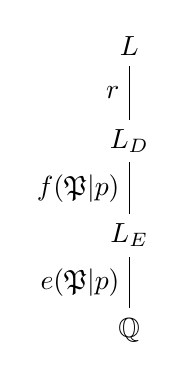
\begin{tikzpicture}[node distance = 1.2cm, auto]
      \node (Q) {$\mathbb{Q}$};
      \node (L_E) [above of=Q] {$L_E$};
      \node (L_D) [above of=L_E] {$L_D$};
      \node (L) [above of=L_D] {$L$};
      \draw[-] (Q) to node {$e(\mathfrak{P}|p)$} (L_E);
      \draw[-] (L_E) to node {$f(\mathfrak{P}|p)$} (L_D);
      \draw[-] (L_D) to node {$r$} (L);
      \end{tikzpicture}
\end{center}

where $[L:\mathbb{Q}] = 6$. From this tower of fields, we may determine the decomposition group. Let $p \in S$. For any $\mathfrak{p}$ lying over $p$, we note that $L/K$ is a Galois extension of degree $2$. Hence there are 3 possibilities for the decomposition of $\mathfrak{p}$ in $L$. Namely
\begin{enumerate}[i.]
\item $r = 2$ and  $e(\mathfrak{P}|\mathfrak{p}) = f(\mathfrak{P}|\mathfrak{p}) = 1$. Then $\mathfrak{p}\mathcal{O}_L = \mathfrak{P}_1\mathfrak{P}_2.$
\item $e(\mathfrak{P}|\mathfrak{p}) = 2$ and $r = f(\mathfrak{P}|\mathfrak{p}) = 1$. Then $\mathfrak{p}\mathcal{O}_L = \mathfrak{P}_1^2.$
\item $f(\mathfrak{P}|\mathfrak{p}) = 2$ and $r = e(\mathfrak{P}|\mathfrak{p}) = 1$. Then $\mathfrak{p}\mathcal{O}_L = \mathfrak{P}_1.$
\end{enumerate}

For $p \in S$, there are $5$ possibilities for the decomposition of $p$ in $K$. In particular,
\begin{enumerate}[1.]
\item $(p)\mathcal{O}_K = \mathfrak{p}_1$ with $e(\mathfrak{p}_1|p) = 1, f(\mathfrak{p}_1|p) = 3$. By the PIRL, it follows that this prime ideal is bounded and therefore does not appear unbounded in \eqref{Eq:TMfactored}.
\item $(p)\mathcal{O}_K = \mathfrak{p}_1^3$ with $e(\mathfrak{p}_1|p) = 3, f(\mathfrak{p}_1|p) = 1$. By the PIRL, it follows that this prime ideal is bounded and therefore does not appear unbounded in \eqref{Eq:TMfactored}.

\item $(p)\mathcal{O}_K = \mathfrak{p}_1 \mathfrak{p}_2$ with $e(\mathfrak{p}_1|p) = f(\mathfrak{p}_1|p) = 1$ and $e(\mathfrak{p}_2|p) = 1, f(\mathfrak{p}_2|p) = 2$.

Looking at the possibilities for the factorization of $\mathfrak{p}_2$ in $L$, we observe
\begin{enumerate}[i.]
\item Since 
\[e(\mathfrak{P}|p) = e(\mathfrak{P}|\mathfrak{p}_2)e(\mathfrak{p}|p) = 1 \quad \text{ and } \quad f(\mathfrak{P}|p) = f(\mathfrak{P}|\mathfrak{p}_2)f(\mathfrak{p}|p) = 2,\]
it follows from $6 = r\cdot e(\mathfrak{P}|p)\cdot f(\mathfrak{P}|p)$ that $r = 3$. Hence
\[(p)\mathcal{O}_L = \mathfrak{P}_1\mathfrak{P}_2\mathfrak{P}_3 \implies |D(\mathfrak{P}_i|p)| = 2.\]
\item Since 
\[e(\mathfrak{P}|p) = e(\mathfrak{P}|\mathfrak{p}_2)e(\mathfrak{p}|p) = 2 \quad \text{ and } \quad f(\mathfrak{P}|p) = f(\mathfrak{P}|\mathfrak{p}_2)f(\mathfrak{p}|p) = 2,\]
it follows from $6 = r\cdot e(\mathfrak{P}|p)\cdot f(\mathfrak{P}|p) = r \cdot 4$ that such a case is not possible.
\item Since 
\[e(\mathfrak{P}|p) = e(\mathfrak{P}|\mathfrak{p}_2)e(\mathfrak{p}|p) = 1 \quad \text{ and } \quad f(\mathfrak{P}|p) = f(\mathfrak{P}|\mathfrak{p}_2)f(\mathfrak{p}|p) = 4,\]
it follows from $6 = r\cdot e(\mathfrak{P}|p)\cdot f(\mathfrak{P}|p) = r \cdot 4$ that such a case is not possible.\end{enumerate}
Now, since
\[e(\mathfrak{P}|p) = 1 \quad \text{ and } \quad f(\mathfrak{P}|p) = 2\]
is the only possible case, we have that $|D(\mathfrak{P}_i|p)| = 2$ for $i = 1,2,3$.

\item $(p)\mathcal{O}_K = \mathfrak{p}_1 \mathfrak{p}_2^2$ with $e(\mathfrak{p}_1|p) = f(\mathfrak{p}_1|p) = 1$ and $e(\mathfrak{p}_2|p) = 2, f(\mathfrak{p}_2|p) = 1$.

Looking at the possibilities for the factorization of $\mathfrak{p}_2$ in $L$, we observe
\begin{enumerate}[i.]
\item Since 
\[e(\mathfrak{P}|p) = e(\mathfrak{P}|\mathfrak{p}_2)e(\mathfrak{p}|p) = 2 \quad \text{ and } \quad f(\mathfrak{P}|p) = f(\mathfrak{P}|\mathfrak{p}_2)f(\mathfrak{p}|p) = 1,\]
it follows from $6 = r\cdot e(\mathfrak{P}|p)\cdot f(\mathfrak{P}|p)$ that $r = 3$. Hence
\[(p)\mathcal{O}_L = \mathfrak{P}_1^2\mathfrak{P}_2^2\mathfrak{P}_3^2 \implies |D(\mathfrak{P}_i|p)| = 2.\]
\item Since 
\[e(\mathfrak{P}|p) = e(\mathfrak{P}|\mathfrak{p}_2)e(\mathfrak{p}|p) = 4 \quad \text{ and } \quad f(\mathfrak{P}|p) = f(\mathfrak{P}|\mathfrak{p}_2)f(\mathfrak{p}|p) = 1,\]
it follows from $6 = r\cdot e(\mathfrak{P}|p)\cdot f(\mathfrak{P}|p) = r \cdot 4$ that such a case is not possible.
\item Since 
\[e(\mathfrak{P}|p) = e(\mathfrak{P}|\mathfrak{p}_2)e(\mathfrak{p}|p) = 2 \quad \text{ and } \quad f(\mathfrak{P}|p) = f(\mathfrak{P}|\mathfrak{p}_2)f(\mathfrak{p}|p) = 2,\]
it follows from $6 = r\cdot e(\mathfrak{P}|p)\cdot f(\mathfrak{P}|p) = r \cdot 4$ that such a case is not possible.\end{enumerate}
Now, since
\[e(\mathfrak{P}|p) = 2 \quad \text{ and } \quad f(\mathfrak{P}|p) = 1\]
is the only possible case, we have that $|D(\mathfrak{P}_i|p)| = 2$ for $i = 1,2,3$.

\item $(p)\mathcal{O}_K = \mathfrak{p}_1 \mathfrak{p}_2\mathfrak{p}_3$ with $e(\mathfrak{p}_i|p) = f(\mathfrak{p}_i|p) = 1$ for $i = 1,2,3$.

Looking at the possibilities for the factorization of $\mathfrak{p}_i$ in $L$, we observe
\begin{enumerate}[i.]
\item Since 
\[e(\mathfrak{P}|p) = e(\mathfrak{P}|\mathfrak{p}_i)e(\mathfrak{p}|p) = 1 \quad \text{ and } \quad f(\mathfrak{P}|p) = f(\mathfrak{P}|\mathfrak{p}_i)f(\mathfrak{p}|p) = 1,\]
it follows from $6 = r\cdot e(\mathfrak{P}|p)\cdot f(\mathfrak{P}|p)$ that $r = 6$. Hence
\[(p)\mathcal{O}_L = \mathfrak{P}_1\mathfrak{P}_2\mathfrak{P}_3\mathfrak{P}_4\mathfrak{P}_5\mathfrak{P}_6 \implies |D(\mathfrak{P}_i|p)| = 1.\]
In this case, the only automorphism $\sigma$ on $L$ such that $\sigma(\mathfrak{P}) = \mathfrak{P}$ is the identity map, hence there can be no cancellation in this case.  
\item Since 
\[e(\mathfrak{P}|p) = e(\mathfrak{P}|\mathfrak{p}_i)e(\mathfrak{p}|p) = 2 \quad \text{ and } \quad f(\mathfrak{P}|p) = f(\mathfrak{P}|\mathfrak{p}_i)f(\mathfrak{p}|p) = 1,\]
it follows from $6 = r\cdot e(\mathfrak{P}|p)\cdot f(\mathfrak{P}|p)$ that $r = 3$. Hence
\[(p)\mathcal{O}_L = \mathfrak{P}_1^2\mathfrak{P}_2^2\mathfrak{P}_3^2 \implies |D(\mathfrak{P}_i|p)| = 2.\]
\item Since 
\[e(\mathfrak{P}|p) = e(\mathfrak{P}|\mathfrak{p}_2)e(\mathfrak{p}|p) = 1 \quad \text{ and } \quad f(\mathfrak{P}|p) = f(\mathfrak{P}|\mathfrak{p}_2)f(\mathfrak{p}|p) = 2,\]
it follows from $6 = r\cdot e(\mathfrak{P}|p)\cdot f(\mathfrak{P}|p)$ that $r = 3$. Hence
\[(p)\mathcal{O}_L = \mathfrak{P}_1\mathfrak{P}_2\mathfrak{P}_3 \implies |D(\mathfrak{P}_i|p)| = 2.\]
\end{enumerate}
\end{enumerate}

From the above list, we observe that we are left to determine whether $D(\mathfrak{P}_i|p)$ having cardinality $2$ can result in $\mathfrak{P}^{(i_0)} = \mathfrak{P}^{(j)}$. We recall that the generating automorphisms of $S_3$ either permute $\theta$ or send $\sqrt{D}$ to $-\sqrt{D}$. If we fix $\theta = \theta_1$, then, in sending $\theta_1$ to $\theta_1$, then we either select an element of $S_3$ that has order 1 (the identity map) or order $2$ ($\tau$). To send $\theta_1$ to $\theta_2$, our choices are either an order $3$ element ($\sigma$) or an order 2 element, $\tau\sigma^2$. Lastly, to send $\theta_1$ to $\theta_3$, we choose either between an order $3$ element, $\sigma^2$, or an order 2 element, $\tau\sigma$. The choice of the automorphisms themselves do not matter so long as $\theta$ is permuted. In other words, we choose $(i_0, j,k)$ so that it forms an order $3$ subgroup of $S_3$. Since only a cardinality $2$ subgroup can map a prime ideal $\mathfrak{P}$ to itself, it follows that this choice of $(i_0,j,k)$ cannot coincide with $D(\mathfrak{P}|p)$ and therefore cannot lead to $\mathfrak{P}^{(i_0)} = \mathfrak{P}^{(j)}$. 
\end{proof}

For the remainder of this paper, we assume that $(i_0,j,k)$ are automorphisms of $L$ selected as in Lemma~\ref{lem:cancellation}.

\begin{lemma}\label{lem:ordpz}
Let $\mathfrak{P}$ be a finite place of $L$ and let $\mathfrak{P}^{(i_0)} = \sigma_{i_0}(\mathfrak{P})$ and $\mathfrak{P}^{(j)} = \sigma_{j}(\mathfrak{P})$, where $\sigma_{i_0}: L \to L$, $\theta \mapsto \theta^{(i_0)}$ and $\sigma_{j}: L \to L$, $\theta \mapsto \theta^{(j)}$ are two automorphisms of $L$. For 
\[\frac{\delta_2}{\lambda}= \prod_{i = 1}^{r}\left( \frac{\varepsilon_i^{(j)}}{\varepsilon_i^{(i_0)}}\right)^{a_i} \prod_{i = 1}^{\nu} \left( \frac{\gamma_i^{(j)}}{\gamma_i^{(i_0)}}\right)^{n_i},\]
we have
\[\ord_{\mathfrak{P}}\left(\frac{\delta_2}{\lambda}\right)=
\begin{cases}
(u_l - r_l)e(\mathfrak{P}^{(j)}|\mathfrak{p}_l^{(j)})	
	& \textnormal{ if } \mathfrak{P}^{(j)} \mid p_l , \ p_l \in \{p_1,\dots, p_{\nu}\}\\
(r_l - u_l)e(\mathfrak{P}^{(i_0)}|\mathfrak{p}_l^{(i_0)})
	& \textnormal{ if } \mathfrak{P}^{(i_0)}\mid p_l, \ p_l \in \{p_1,\dots, p_{\nu}\}\\
0 	& \textnormal{ otherwise}.
\end{cases}\]
\end{lemma}
\begin{proof}

By Lemma~\ref{lem:cancellation}, we have 
\[\left( \frac{\gamma_i^{(j)}}{\gamma_i^{(i_0)}}\right)\mathcal{O}_L 
	 = \left(\prod_{\mathfrak{P}\mid\mathfrak{p}_1} \frac{\mathfrak{P}^{(j) \ e(\mathfrak{P}^{(j)}\mid\mathfrak{p}_1^{(j)})}}{\mathfrak{P}^{(i_0) \ e(\mathfrak{P}^{(i_0)}\mid\mathfrak{p}^{(i_0)}_1)}}\right)^{a_{1i}} \cdots \left(\prod_{\mathfrak{P}\mid\mathfrak{p}_{\nu}} \frac{\mathfrak{P}^{(j) \ e(\mathfrak{P}^{(j)}\mid\mathfrak{p}^{(j)}_{\nu})}}{\mathfrak{P}^{(i_0) \ e(\mathfrak{P}^{(i_0)}\mid\mathfrak{p}^{(i_0)}_{\nu})}}\right)^{a_{\nu i}}.\]
Hence
\begin{align*}
\left(\frac{\delta_2}{\lambda}\right)\mathcal{O}_L
	& = \left( \frac{\gamma_1^{(j)}}{\gamma_1^{(i_0)}}\right)^{n_1}\cdots \left( \frac{\gamma_{\nu}^{(j)}}{\gamma_{\nu}^{(i_0)}}\right)^{n_{\nu}} \mathcal{O}_L\\
	& = \left(\prod_{\mathfrak{P}\mid\mathfrak{p}_1} \frac{\mathfrak{P}^{(j) \ e(\mathfrak{P}^{(j)}\mid\mathfrak{p}_1^{(j)})}}{\mathfrak{P}^{(i_0) \ e(\mathfrak{P}^{(i_0)}\mid\mathfrak{p}^{(i_0)}_1)}}\right)^{n_1a_{11}} \cdots \left(\prod_{\mathfrak{P}\mid\mathfrak{p}_{\nu}} \frac{\mathfrak{P}^{(j) \ e(\mathfrak{P}^{(j)}\mid\mathfrak{p}^{(j)}_{\nu})}}{\mathfrak{P}^{(i_0) \ e(\mathfrak{P}^{(i_0)}\mid\mathfrak{p}^{(i_0)}_{\nu})}}\right)^{n_1a_{\nu 1}} \cdots \\
	& \quad \quad \cdots 
\left(\prod_{\mathfrak{P}\mid\mathfrak{p}_1} \frac{\mathfrak{P}^{(j) \ e(\mathfrak{P}^{(j)}\mid\mathfrak{p}_1^{(j)})}}{\mathfrak{P}^{(i_0) \ e(\mathfrak{P}^{(i_0)}\mid\mathfrak{p}^{(i_0)}_1)}}\right)^{n_{\nu}a_{1\nu}} \cdots \left(\prod_{\mathfrak{P}\mid\mathfrak{p}_{\nu}} \frac{\mathfrak{P}^{(j) \ e(\mathfrak{P}^{(j)}\mid\mathfrak{p}^{(j)}_{\nu})}}{\mathfrak{P}^{(i_0) \ e(\mathfrak{P}^{(i_0)}\mid\mathfrak{p}^{(i_0)}_{\nu})}}\right)^{n_{\nu} a_{\nu \nu}} \\
	& = \left(\prod_{\mathfrak{P}\mid\mathfrak{p}_1} \frac{\mathfrak{P}^{(j) \ e(\mathfrak{P}^{(j)}\mid\mathfrak{p}_1^{(j)})}}{\mathfrak{P}^{(i_0) \ e(\mathfrak{P}^{(i_0)}\mid\mathfrak{p}^{(i_0)}_1)}}\right)^{\sum_{i = 1}^\nu n_ia_{1i}} \cdots \left(\prod_{\mathfrak{P}\mid\mathfrak{p}_{\nu}} \frac{\mathfrak{P}^{(j) \ e(\mathfrak{P}^{(j)}\mid\mathfrak{p}^{(j)}_{\nu})}}{\mathfrak{P}^{(i_0) \ e(\mathfrak{P}^{(i_0)}\mid\mathfrak{p}^{(i_0)}_{\nu})}}\right)^{\sum_{i=1}^{\nu} n_ia_{\nu i}}\\
	& = \left(\prod_{\mathfrak{P}\mid\mathfrak{p}_1} \frac{\mathfrak{P}^{(j) \ e(\mathfrak{P}^{(j)}\mid\mathfrak{p}_1^{(j)})}}{\mathfrak{P}^{(i_0) \ e(\mathfrak{P}^{(i_0)}\mid\mathfrak{p}^{(i_0)}_1)}}\right)^{u_1 - r_1} \cdots \left(\prod_{\mathfrak{P}\mid\mathfrak{p}_{\nu}} \frac{\mathfrak{P}^{(j) \ e(\mathfrak{P}^{(j)}\mid\mathfrak{p}^{(j)}_{\nu})}}{\mathfrak{P}^{(i_0) \ e(\mathfrak{P}^{(i_0)}\mid\mathfrak{p}^{(i_0)}_{\nu})}}\right)^{u_{\nu} - r_{\nu}}\\
\end{align*}
and so
\[\ord_{\mathfrak{P}}\left( \frac{\delta_2}{\lambda}\right)=
\begin{cases}
(u_l - r_l)e(\mathfrak{P}^{(j)}|\mathfrak{p}_l^{(j)})	
	& \textnormal{ if } \mathfrak{P}^{(j)} \mid p_l , \ p_l \in \{p_1,\dots, p_{\nu}\}\\
(r_l - u_l)e(\mathfrak{P}^{(i_0)}|\mathfrak{p}_l^{(i_0)})
	& \textnormal{ if } \mathfrak{P}^{(i_0)}\mid p_l, \ p_l \in \{p_1,\dots, p_{\nu}\}\\
0 	& \textnormal{ otherwise}.
\end{cases}\]
\end{proof}

Let $\log^+(\cdot)$ denote the real valued function $\max(\log(\cdot), 0)$ on $\mathbb{R}_{\geq 0}$. 

\begin{proposition}\label{prop:heightdecomp}
The height $h\left(\frac{\delta_2}{\lambda}\right)$ admits a decomposition
\[h\left(\frac{\delta_2}{\lambda}\right) = \frac{1}{[K:\mathbb{Q}]}\sum_{l = 1}^{\nu} \log(p_l)|u_l - r_l| + \frac{1}{[L:\mathbb{Q}]}\sum_{w :L \to \mathbb{C}} \log \max \left\{ \left|w\left(\frac{\delta_2}{\lambda}\right)\right|, 1\right\} \]

Further, if $\deg{g(t)}=3$ then 
\[\sum_{w :L \to \mathbb{C}} \log \max \left\{ \left|w\left(\frac{\delta_2}{\lambda}\right)\right|, 1\right\} = 
\begin{cases}
2\max_{w:L\to \mathbb{C}} \log \max \left\{ \left|w\left(\frac{\delta_2}{\lambda}\right)\right|, 1\right\} & \text{ if } \sqrt{\Delta}\notin\mathbb{Q} \\
\max_{w:L\to \mathbb{C}}\sum_{w :L \to \mathbb{C}} \log \max \left\{ \left|w\left(\frac{\delta_2}{\lambda}\right)\right|, 1\right\} & \text{ if } \sqrt{\Delta}\in\mathbb{Q} \\
\end{cases}\]
when one can choose $(i_0),(j), (k) : L \to \mathbb{C}$ such that $\mathfrak{p}_{p}^{(j)} \neq \mathfrak{p}_{p}^{(i_0)}$ for all $p \in S$. 
\end{proposition}

\begin{proof}[Proof of Proposition~\ref{prop:heightdecomp}]Since $\frac{\delta_2}{\lambda} \in L$, the definition of the absolute logarithmic Weil height gives
\[h\left(\frac{\delta_2}{\lambda}\right)=\frac{1}{[L:\mathbb{Q}]}\sum_{w \in M_L} \log \max \left\{ \left\|\frac{\delta_2}{\lambda}\right\|_{w}, 1\right\}\]
where $||z||_w$ are the usual norms and $M_L$ is a set of inequivalent absolute values on $L$. 

In particular, if $w: L \to \mathbb{C}$ is an infinite place, we obtain
\[ \log \max \left\{ \left\|\frac{\delta_2}{\lambda}\right\|_{w}, 1\right\} = \log \max \left\{ \left|w\left(\frac{\delta_2}{\lambda}\right)\right|, 1\right\}.\]

Now, for $z = \frac{\delta_2}{\lambda}$ and $w = \mathfrak{P}$ a finite place, we have
\[ \log \max \{ \|z\|_{w}, 1\} = \max \left\{ \log\left(\frac{1}{N(\mathfrak{P})^{\ord_{\mathfrak{P}}(z)}} \right), 0\right\}. \]
By Lemma~\ref{lem:ordpz}, 
\[\ord_{\mathfrak{P}}\left( \frac{\delta_2}{\lambda}\right)=
\begin{cases}
(u_l - r_l)e(\mathfrak{P}^{(j)}|\mathfrak{p}_l^{(j)})	
	& \textnormal{ if } \mathfrak{P}^{(j)} \mid p_l , \ p_l \in \{p_1,\dots, p_{\nu}\}\\
(r_l - u_l)e(\mathfrak{P}^{(i_0)}|\mathfrak{p}_l^{(i_0)})
	& \textnormal{ if } \mathfrak{P}^{(i_0)}\mid p_l, \ p_l \in \{p_1,\dots, p_{\nu}\}\\
0 	& \textnormal{ otherwise}.
\end{cases}\]
That is, for $\mathfrak{P}^{(j)}\mid p_l$ where $p_l \in \{p_1, \dots, p_{\nu}\}$, we have
\begin{align*}
 \log \max \{ ||z||_{w}, 1\}	
 	& = \max \left\{ \log\left(\frac{1}{N(\mathfrak{P})^{\ord_{\mathfrak{P}}(z)}} \right), 0\right\}\\
	& = \max \left\{ \log\left(\frac{1}{N(\mathfrak{P})^{(u_l - r_l)e(\mathfrak{P}^{(j)}|\mathfrak{p}_l^{(j)})}} \right), 0\right\}\\
	& = \max \left\{ \log\left(\frac{1}{p_l^{(u_l - r_l)f(\mathfrak{P}^{(j)}\mid p_l)e(\mathfrak{P}^{(j)}|\mathfrak{p}_l^{(j)})}} \right), 0\right\}\\
	& = \max \left\{ -(u_l - r_l)f(\mathfrak{P}^{(j)}\mid p_l)e(\mathfrak{P}^{(j)}|\mathfrak{p}_l^{(j)})\log(p_l), 0\right\}.
\end{align*}
For $p_l \in \{p_1, \dots, p_{\nu}\}$, there is 1 unique prime ideal $\mathfrak{p}_1$ in the ideal equation \eqref{Eq:TMfactored} lying above $p_l$ in $K$. Hence, each $\mathfrak{P}$ lying over $p_l$ must also lie over $\mathfrak{p}_l$. Now, 
\begin{align*}
\sum_{\mathfrak{P}^{(j)} \mid \mathfrak{p}_l^{(j)}} \log \max \left\{ \left\|\frac{\delta_2}{\lambda}\right\|_{w}, 1\right\}
	& = \sum_{\mathfrak{P}^{(j)} \mid \mathfrak{p}_l^{(j)}} \max \left\{ -(u_l - r_l)f(\mathfrak{P}^{(j)}\mid p_l)e(\mathfrak{P}^{(j)}|\mathfrak{p}_l^{(j)})\log(p_l), 0\right\}\\
	& = \max \left\{ (r_l - u_l)\log(p_l), 0\right\}\sum_{\mathfrak{P}^{(j)} \mid \mathfrak{p}_l^{(j)}}f(\mathfrak{P}^{(j)}\mid p_l)e(\mathfrak{P}^{(j)}|\mathfrak{p}_l^{(j)})\\
	& = \max \left\{ (r_l - u_l)\log(p_l), 0\right\}\sum_{\mathfrak{P}^{(j)} \mid \mathfrak{p}_l^{(j)}}f(\mathfrak{P}^{(j)}\mid \mathfrak{p}_l^{(j)})f(\mathfrak{p}_l^{(j)}\mid p_l)e(\mathfrak{P}^{(j)}|\mathfrak{p}_l^{(j)})\\
	& = \max \left\{ (r_l - u_l)\log(p_l), 0\right\}f(\mathfrak{p}_l^{(j)}\mid p_l)\sum_{\mathfrak{P}^{(j)} \mid \mathfrak{p}_l^{(j)}}f(\mathfrak{P}^{(j)}\mid \mathfrak{p}_l^{(j)})e(\mathfrak{P}^{(j)}|\mathfrak{p}_l^{(j)})\\
	& = \max \left\{ (r_l - u_l)\log(p_l), 0\right\}f(\mathfrak{p}_l^{(j)}\mid p_l)[L:\mathbb{Q}(\theta^{(j)})]\\
	& = \max \left\{ (r_l - u_l)\log(p_l), 0\right\}f(\mathfrak{p}_l^{(j)}\mid p_l)[L:K].
\end{align*}
where the last inequality follows from $K = \mathbb{Q}(\theta) \cong \mathbb{Q}(\theta^{(j)})$

Similarly, for $\mathfrak{P}^{(i_0)}\mid p_l$ where $p_l \in \{p_1, \dots, p_{\nu}\}$, we have
\begin{align*}
 \log \max \{ \|z\|_{w}, 1\}	
 	& = \max \left\{ \log\left(\frac{1}{N(\mathfrak{P})^{\ord_{\mathfrak{P}}(z)}} \right), 0\right\}\\
	& = \max \left\{ \log\left(\frac{1}{N(\mathfrak{P})^{(r_l - u_l)e(\mathfrak{P}^{(i_0)}|\mathfrak{p}_l^{(i_0)})}} \right), 0\right\}\\
	& = \max \left\{ \log\left(\frac{1}{p_l^{(r_l - u_l)f(\mathfrak{P}^{(i_0)}\mid p_l)e(\mathfrak{P}^{(i_0)}|\mathfrak{p}_l^{(i_0)})}} \right), 0\right\}\\
	& = \max \left\{ -(r_l - u_l)f(\mathfrak{P}^{(i_0)}\mid p_l)e(\mathfrak{P}^{(i_0)}|\mathfrak{p}_l^{(i_0)})\log(p_l), 0\right\},
\end{align*}
and so
\begin{align*}
\sum_{\mathfrak{P}^{(i_0)} \mid \mathfrak{p}_l^{(i_0)}} \log \max \left\{ \left\|\frac{\delta_2}{\lambda}\right\|_{w}, 1\right\}
	& = \max \left\{ (u_l - r_l)\log(p_l), 0\right\}f(\mathfrak{p}_l^{(i_0)}\mid p_l)[L:K].
\end{align*}

Lastly, if $w = \mathfrak{P}$ such that $\mathfrak{P} \neq \mathfrak{P}^{(i_0)},  \mathfrak{P}^{(j)}$, we have
\begin{align*}
 \log \max \{ \|z\|_{w}, 1\}	
 	& = \max \left\{ \log\left(\frac{1}{N(\mathfrak{P})^{\ord_{\mathfrak{P}}(z)}} \right), 0\right\}\\
	& = \max \left\{ \log\left(\frac{1}{N(\mathfrak{P})^{0}} \right), 0\right\}\\
	& = 0.
\end{align*}

Now, we have 
\begin{align*}
h\left(\frac{\delta_2}{\lambda}\right)
	& =\frac{1}{[L:\mathbb{Q}]}\sum_{w \in M_L} \log \max \left\{ \left\|\frac{\delta_2}{\lambda}\right\|_{w}, 1\right\}\\
	& = \frac{1}{[L:\mathbb{Q}]}\sum_{w :L \to \mathbb{C}} \log \max \left\{ \left|w\left(\frac{\delta_2}{\lambda}\right)\right|, 1\right\} + \frac{1}{[L:\mathbb{Q}]}\sum_{\mathfrak{P} \in \mathcal{O}_L \text{ finite }} \log \max \left\{ \left\|\frac{\delta_2}{\lambda}\right\|_{\mathfrak{P}}, 1\right\},
\end{align*}
where
\begin{align*}
& \sum_{\mathfrak{P} \in \mathcal{O}_L \text{ finite }} \log \max \left\{ \left\|\frac{\delta_2}{\lambda}\right\|_{w}, 1\right\} \\
	& = \sum_{l = 1}^{\nu} \left(\sum_{\mathfrak{P}^{(j)} \mid \mathfrak{p}_l^{(j)}} \log \max \left\{ \left\|\frac{\delta_2}{\lambda}\right\|_{w}, 1\right\} + \sum_{\mathfrak{P}^{(i_0)} \mid \mathfrak{p}_l^{(i_0)}} \log \max \left\{ \left\|\frac{\delta_2}{\lambda}\right\|_{w}, 1\right\}\right)\\
	& = \sum_{l = 1}^{\nu} \left(\max \left\{ (r_l - u_l)\log(p_l), 0\right\}f(\mathfrak{p}_l^{(j)}\mid p_l)[L:K] + \max \left\{ (u_l - r_l)\log(p_l), 0\right\}f(\mathfrak{p}_l^{(i_0)}\mid p_l)[L:K]\right)\\
	& =  [L:K]\sum_{l = 1}^{\nu} \log(p_l)\left(\max \left\{ -(u_l - r_l), 0\right\}+ \max \left\{ (u_l - r_l), 0\right\}\right)\\
	& =  [L:K]\sum_{l = 1}^{\nu} \log(p_l)\max \left\{ -(u_l - r_l), (u_l - r_l)\right\}\\
	& =  [L:K]\sum_{l = 1}^{\nu} \log(p_l)|u_l - r_l|.
\end{align*}
Here, we recall that $K = \mathbb{Q}(\theta) \cong \mathbb{Q}(\theta^{(i_0)}) \cong \mathbb{Q}(\theta^{(j)})$ and therefore 
\[f(\mathfrak{p}_l^{(i_0)}\mid p_l) = f(\mathfrak{p}_l^{(j)}\mid p_l) = f(\mathfrak{p}_l\mid p_l) = 1.\]
Altogether, we have
\begin{align*}
h\left(\frac{\delta_2}{\lambda}\right)
	& =\frac{1}{[L:\mathbb{Q}]}\sum_{w \in M_L} \log \max \left\{ \left\|\frac{\delta_2}{\lambda}\right\|_{w}, 1\right\}\\
	& = \frac{1}{[L:\mathbb{Q}]}\sum_{w :L \to \mathbb{C}} \log \max \left\{ \left|w\left(\frac{\delta_2}{\lambda}\right)\right|, 1\right\} + \frac{1}{[L:\mathbb{Q}]}\sum_{\mathfrak{P} \in \mathcal{O}_L \text{ finite }} \log \max \left\{ \left\|\frac{\delta_2}{\lambda}\right\|_{\mathfrak{P}}, 1\right\}\\
	& = \frac{1}{[L:\mathbb{Q}]}\sum_{w :L \to \mathbb{C}} \log \max \left\{ \left|w\left(\frac{\delta_2}{\lambda}\right)\right|, 1\right\} + \frac{1}{[K:\mathbb{Q}]}\sum_{l = 1}^{\nu} \log(p_l)|u_l - r_l|\\
	& = \frac{1}{[L:\mathbb{Q}]}\sum_{w :L \to \mathbb{C}} \log \max \left\{ \left|w\left(\frac{\delta_2}{\lambda}\right)\right|, 1\right\} + \frac{1}{[K:\mathbb{Q}]}\log\left(p_1^{|u_1 - r_1|} \cdots p_{\nu}^{|u_{\nu} - r_{\nu}|}\right)
\end{align*}

To prove the last statement, we first assume that $\sqrt{\Delta}\in\mathbb{Q}$. Then $L=\mathbb{Q}(\theta, \sqrt{\Delta}) = \mathbb{Q}(\theta) = K$ and the Galois group of $L/\mathbb{Q}$ is the alternating group $A_3$. Hence the Galois group is generated by $\sigma$, which takes $\theta$ to one of the other roots of $g(t)$. In particular, 
\[\Gal(L/\mathbb{Q}) = \{ \text{id}_\text{L}, \sigma, \sigma^2\},\]
where
\begin{align*}
\text{id}_{\text{L}}: 
\begin{cases}
\theta_1 \mapsto \theta_1\\
\theta_2 \mapsto \theta_2\\
\theta_3 \mapsto \theta_3\\
\sqrt{D} \mapsto \sqrt{D}
\end{cases}
& \quad ,
\sigma: 
\begin{cases}
\theta_1 \mapsto \theta_2\\
\theta_2 \mapsto \theta_3\\
\theta_3 \mapsto \theta_1\\
\sqrt{D} \mapsto \sqrt{D}
\end{cases}
& \quad ,
\sigma^2: 
\begin{cases}
\theta_1 \mapsto \theta_3\\
\theta_2 \mapsto \theta_1\\
\theta_3 \mapsto \theta_2\\
\sqrt{D} \mapsto \sqrt{D}
\end{cases},
\end{align*}
Writing $j = 1, i_0 = 2$ and $k = 3$, the orbit of 
\[\frac{\delta_2}{\lambda}= \prod_{i = 1}^{r}\left( \frac{\varepsilon_i^{(1)}}{\varepsilon_i^{(2)}}\right)^{a_i} \prod_{i = 1}^{\nu} \left( \frac{\gamma_i^{(1)}}{\gamma_i^{(2)}}\right)^{n_i}\in L\]
is
\[\left\{ \prod_{i = 1}^{r}\left( \frac{\varepsilon_i^{(1)}}{\varepsilon_i^{(2)}}\right)^{a_i} \prod_{i = 1}^{\nu} \left( \frac{\gamma_i^{(1)}}{\gamma_i^{(2)}}\right)^{n_i}, 
	\prod_{i = 1}^{r}\left( \frac{\varepsilon_i^{(2)}}{\varepsilon_i^{(3)}}\right)^{a_i} \prod_{i = 1}^{\nu} \left( \frac{\gamma_i^{(2)}}{\gamma_i^{(3)}}\right)^{n_i}, 
	\prod_{i = 1}^{r}\left( \frac{\varepsilon_i^{(3)}}{\varepsilon_i^{(1)}}\right)^{a_i} \prod_{i = 1}^{\nu} \left( \frac{\gamma_i^{(3)}}{\gamma_i^{(1)}}\right)^{n_i}\right\}.\]
We choose $a,b,c\in\{1,2,3\}$ such that 
\[ \left|\prod_{i = 1}^{r}\left( \varepsilon_i^{(a)}\right)^{a_i} \prod_{i = 1}^{\nu} \left( \gamma_i^{(a)}\right)^{n_i}\right| \geq
	\left|\prod_{i = 1}^{r}\left( \varepsilon_i^{(b)}\right)^{a_i} \prod_{i = 1}^{\nu} \left( \gamma_i^{(b)}\right)^{n_i}\right| \geq
	\left|\prod_{i = 1}^{r}\left( \varepsilon_i^{(c)}\right)^{a_i} \prod_{i = 1}^{\nu} \left( \gamma_i^{(c)}\right)^{n_i}\right|.\]
Then we obtain
\begin{align*}
\sum_{w :L \to \mathbb{C}} \log \max \left\{ \left|w\left(\frac{\delta_2}{\lambda}\right)\right|, 1\right\}
	& = \log \max \left\{ \left|\text{id}_L\left(\frac{\delta_2}{\lambda}\right)\right|, 1\right\} 
		+ \log \max \left\{ \left|\sigma\left(\frac{\delta_2}{\lambda}\right)\right|,1\right\} \\
		& \quad+ \log \max \left\{ \left|\sigma^2\left(\frac{\delta_2}{\lambda}\right)\right|, 1\right\}\\
	& = \log \max \left\{ \left|\prod_{i = 1}^{r}\left( \frac{\varepsilon_i^{(a)}}{\varepsilon_i^{(b)}}\right)^{a_i} \prod_{i = 1}^{\nu} \left( \frac{\gamma_i^{(a)}}{\gamma_i^{(b)}}\right)^{n_i} \right|, 1\right\} \\
		& \quad + \log \max \left\{ \left|\ \prod_{i = 1}^{r}\left( \frac{\varepsilon_i^{(b)}}{\varepsilon_i^{(c)}}\right)^{a_i} \prod_{i = 1}^{\nu} \left( \frac{\gamma_i^{(b)}}{\gamma_i^{(c)}}\right)^{n_i} \right|,1\right\} \\
		& \quad+ \log \max \left\{ \left| \prod_{i = 1}^{r}\left( \frac{\varepsilon_i^{(c)}}{\varepsilon_i^{(a)}}\right)^{a_i} \prod_{i = 1}^{\nu} \left( \frac{\gamma_i^{(c)}}{\gamma_i^{(a)}}\right)^{n_i} \right|, 1\right\}\\
	& = \log  \left|\prod_{i = 1}^{r}\left( \frac{\varepsilon_i^{(a)}}{\varepsilon_i^{(b)}}\right)^{a_i} \prod_{i = 1}^{\nu} \left( \frac{\gamma_i^{(a)}}{\gamma_i^{(b)}}\right)^{n_i} \right| \\
		& \quad + \log \left|\ \prod_{i = 1}^{r}\left( \frac{\varepsilon_i^{(b)}}{\varepsilon_i^{(c)}}\right)^{a_i} \prod_{i = 1}^{\nu} \left( \frac{\gamma_i^{(b)}}{\gamma_i^{(c)}}\right)^{n_i} \right| \\
	& = \log  \left|\prod_{i = 1}^{r}\left( \frac{\varepsilon_i^{(a)}}{\varepsilon_i^{(c)}}\right)^{a_i} \prod_{i = 1}^{\nu} \left( \frac{\gamma_i^{(a)}}{\gamma_i^{(c)}}\right)^{n_i} \right|.
\end{align*}
Hence it follows that
\[\sum_{w :L \to \mathbb{C}} \log \max \left\{ \left|w\left(\frac{\delta_2}{\lambda}\right)\right|, 1\right\} = 
\max_{w:L\to \mathbb{C}}\sum_{w :L \to \mathbb{C}} \log \max \left\{ \left|w\left(\frac{\delta_2}{\lambda}\right)\right|, 1\right\}.\]

It remains to consider the case when $\sqrt{\Delta} \notin \mathbb{Q}$. Then the Galois group of $L/\mathbb{Q}$ is the symmetric group $S_3$. We now write $j = 1, i_0 = 2,$ and $k = 3$, the orbit of 
\[\frac{\delta_2}{\lambda}= \prod_{i = 1}^{r}\left( \frac{\varepsilon_i^{(1)}}{\varepsilon_i^{(2)}}\right)^{a_i} \prod_{i = 1}^{\nu} \left( \frac{\gamma_i^{(1)}}{\gamma_i^{(2)}}\right)^{n_i}\in L\]
is
\begin{align*}
& \left\{ \prod_{i = 1}^{r}\left( \frac{\varepsilon_i^{(1)}}{\varepsilon_i^{(2)}}\right)^{a_i} \prod_{i = 1}^{\nu} \left( \frac{\gamma_i^{(1)}}{\gamma_i^{(2)}}\right)^{n_i} , 
	\prod_{i = 1}^{r}\left( \frac{\varepsilon_i^{(2)}}{\varepsilon_i^{(3)}}\right)^{a_i} \prod_{i = 1}^{\nu} \left( \frac{\gamma_i^{(2)}}{\gamma_i^{(3)}}\right)^{n_i}, 
	\prod_{i = 1}^{r}\left( \frac{\varepsilon_i^{(3)}}{\varepsilon_i^{(1)}}\right)^{a_i} \prod_{i = 1}^{\nu} \left( \frac{\gamma_i^{(3)}}{\gamma_i^{(1)}}\right)^{n_i} \right. \\
	& \quad \left. \prod_{i = 1}^{r}\left( \frac{\varepsilon_i^{(3)}}{\varepsilon_i^{(2)}}\right)^{a_i} \prod_{i = 1}^{\nu} \left( \frac{\gamma_i^{(3)}}{\gamma_i^{(2)}}\right)^{n_i} , 
	\prod_{i = 1}^{r}\left( \frac{\varepsilon_i^{(1)}}{\varepsilon_i^{(3)}}\right)^{a_i} \prod_{i = 1}^{\nu} \left( \frac{\gamma_i^{(1)}}{\gamma_i^{(3)}}\right)^{n_i}, 
	\prod_{i = 1}^{r}\left( \frac{\varepsilon_i^{(2)}}{\varepsilon_i^{(1)}}\right)^{a_i} \prod_{i = 1}^{\nu} \left( \frac{\gamma_i^{(2)}}{\gamma_i^{(1)}}\right)^{n_i} \right\}.
\end{align*}
We choose $a,b,c\in\{1,2,3\}$ such that 
\[ \left|\prod_{i = 1}^{r}\left( \varepsilon_i^{(a)}\right)^{a_i} \prod_{i = 1}^{\nu} \left( \gamma_i^{(a)}\right)^{n_i}\right| \geq
	\left|\prod_{i = 1}^{r}\left( \varepsilon_i^{(b)}\right)^{a_i} \prod_{i = 1}^{\nu} \left( \gamma_i^{(b)}\right)^{n_i}\right| \geq
	\left|\prod_{i = 1}^{r}\left( \varepsilon_i^{(c)}\right)^{a_i} \prod_{i = 1}^{\nu} \left( \gamma_i^{(c)}\right)^{n_i}\right|.\]
Then we obtain
\begin{align*}
\sum_{w :L \to \mathbb{C}} \log \max \left\{ \left|w\left(\frac{\delta_2}{\lambda}\right)\right|, 1\right\}
	& = \log \max \left\{ \left|\text{id}_L\left(\frac{\delta_2}{\lambda}\right)\right|, 1\right\} 
		+ \log \max \left\{ \left|\sigma\left(\frac{\delta_2}{\lambda}\right)\right|,1\right\} \\
		& \quad+ \log \max \left\{ \left|\sigma^2\left(\frac{\delta_2}{\lambda}\right)\right|, 1\right\} + \log \max \left\{ \left|\tau\left(\frac{\delta_2}{\lambda}\right)\right|, 1\right\}\\
		& \quad+ \log \max \left\{ \left|\tau\sigma\left(\frac{\delta_2}{\lambda}\right)\right|, 1\right\} + \log \max \left\{ \left|\tau\sigma^2\left(\frac{\delta_2}{\lambda}\right)\right|, 1\right\}\\
	& = \log \left|\prod_{i = 1}^{r}\left( \frac{\varepsilon_i^{(a)}}{\varepsilon_i^{(b)}}\right)^{a_i} \prod_{i = 1}^{\nu} \left( \frac{\gamma_i^{(a)}}{\gamma_i^{(b)}}\right)^{n_i} \right|\\
		& \quad + \log \left|\ \prod_{i = 1}^{r}\left( \frac{\varepsilon_i^{(b)}}{\varepsilon_i^{(c)}}\right)^{a_i} \prod_{i = 1}^{\nu} \left( \frac{\gamma_i^{(b)}}{\gamma_i^{(c)}}\right)^{n_i} \right|\\
		& \quad+ \log \left| \prod_{i = 1}^{r}\left( \frac{\varepsilon_i^{(a)}}{\varepsilon_i^{(c)}}\right)^{a_i} \prod_{i = 1}^{\nu} \left( \frac{\gamma_i^{(a)}}{\gamma_i^{(c)}}\right)^{n_i} \right|\\
	& = 2\log  \left|\prod_{i = 1}^{r}\left( \frac{\varepsilon_i^{(a)}}{\varepsilon_i^{(c)}}\right)^{a_i} \prod_{i = 1}^{\nu} \left( \frac{\gamma_i^{(a)}}{\gamma_i^{(c)}}\right)^{n_i} \right|.
\end{align*}
Hence it follows that
\[\sum_{w :L \to \mathbb{C}} \log \max \left\{ \left|w\left(\frac{\delta_2}{\lambda}\right)\right|, 1\right\} = 
2\max_{w:L\to \mathbb{C}}\sum_{w :L \to \mathbb{C}} \log \max \left\{ \left|w\left(\frac{\delta_2}{\lambda}\right)\right|, 1\right\}.\]
\end{proof}

%---------------------------------------------------------------------------------------------------------------------------------------------%
\subsection{Initial height bounds}

Recall that we seek solutions to
\begin{equation*}
\lambda = \delta_1 \prod_{i = 1}^r\left( \frac{\varepsilon_i^{(k)}}{\varepsilon_i^{(j)}}\right)^{a_i}\prod_{i = 1}^{\nu} \left( \frac{\gamma_i^{(k)}}{\gamma_i^{(j)}}\right)^{n_i} - 1 = \delta_2 \prod_{i = 1}^{r}\left( \frac{\varepsilon_i^{(i_0)}}{\varepsilon_i^{(j)}}\right)^{a_i} \prod_{i = 1}^{\nu} \left( \frac{\gamma_i^{(i_0)}}{\gamma_i^{(j)}}\right)^{n_i},
\end{equation*}
where
\[\delta_1 = \frac{\theta^{(i_0)} - \theta^{(j)}}{\theta^{(i_0)} - \theta^{(k)}}\cdot\frac{\alpha^{(k)}\zeta^{(k)}}{\alpha^{(j)}\zeta^{(j)}}, \quad \delta_2 = \frac{\theta^{(j)} - \theta^{(k)}}{\theta^{(k)} - \theta^{(i_0)}}\cdot \frac{\alpha^{(i_0)}\zeta^{(i_0)}}{\alpha^{(j)}\zeta^{(j)}}\]
are constants and $r = 1$ or $r = 2$. 

In Rafael's notation, let
\[y =  \prod_{i = 1}^r\left( \frac{\varepsilon_i^{(k)}}{\varepsilon_i^{(j)}}\right)^{a_i}\prod_{i = 1}^{\nu} \left( \frac{\gamma_i^{(k)}}{\gamma_i^{(j)}}\right)^{n_i}, \quad 
x = \prod_{i = 1}^{r}\left( \frac{\varepsilon_i^{(i_0)}}{\varepsilon_i^{(j)}}\right)^{a_i} \prod_{i = 1}^{\nu} \left( \frac{\gamma_i^{(i_0)}}{\gamma_i^{(j)}}\right)^{n_i}\]
so that our equation is
\[\delta_1y - 1 = \delta_2x.\]
Equivalently, letting $\mu_0 = \delta_1$ and $\lambda_0 = \delta_2$, we arrive at
\[\mu_0y - \lambda_0x = 1,\]
just as in Rafael's notation. 

Returning to our notation, we see that 
\begin{align*}
\lambda 	& = \delta_2 \prod_{i = 1}^{r}\left( \frac{\varepsilon_i^{(i_0)}}{\varepsilon_i^{(j)}}\right)^{a_i} \prod_{i = 1}^{\nu} \left( \frac{\gamma_i^{(i_0)}}{\gamma_i^{(j)}}\right)^{n_i}\\
		& = \delta_2 x\\
		& = \lambda_0 x.
\end{align*}
Hence, let $z:= \frac{1}{x} = \frac{\delta_2}{\lambda}$.

Now, let $\Sigma$ denote the set of pairs $(x,y)$ satisfying the equation 
\[\mu_0y - \lambda_0x = 1.\]
That is, let $\Sigma$ denote the set of tuples $(n_1, \dots, n_{\nu}, a_1, \dots, a_r)$ giving $x,y$ which satisfy
\[\mu_0y - \lambda_0x = 1.\]

Let $l,h\in\mathbb{R}^{S^*}$ with $0\leq l\leq h$. Then we define $\Sigma(l,h)$ as the set of all $(x,y)\in \Sigma$ such that $\left(h_v\left(\frac{\delta_2}{\lambda}\right)\right)\leq h$ and such that $\left(h_v\left(\frac{\delta_2}{\lambda}\right)\right)\nleq l$, 
\[\Sigma(l,h) = \{(x,y) \in \Sigma \ | \ (h_v(z))\leq h \text{ and } (h_v(z))\nleq l\}.\]
Since we are comparing vectors, we note that $(h_v(z))\nleq l$ does not necessarily mean that $l < (h_v(z))$. Instead, this means that not \textit{all} coordinates $h_v(z)$ satisfy $h_v(z) \leq l_v$, and hence there is at least one coordinate for which $h_v(z) > l_v$.

Here we write $\Sigma(h)=\Sigma(l,h)$ if $l=0$.  
\[\Sigma(h) = \Sigma(0,h)= \{(x,y) \in \Sigma \ | \ (h_v(z))\leq h \text{ and }  (h_v(z))\nleq 0 \},\]
so that at least one coordinate satisfies $h_v(z) > 0$.

Further, for each $w\in S^*$, we denote by $\Sigma_w(l,h)$ the set of all $(x,y)\in\Sigma(h)$ such that $h_w(z)>l_w$. 
\begin{align*}
\Sigma_w(l,h)	& = \{(x,y) \in \Sigma(h) \ | \ h_w(z)>l_w \} \\
			& = \{(x,y) \in \Sigma \ | \ (h_v(z))\leq h \text{ and }  (h_v(z))\nleq 0 \text{ and } h_w(z)>l_w\}.
\end{align*}

Recall that 
\[f(X,Y) = X^3 + C_1 X^{2}Y + C_2XY^2 + C_3Y^3 = c p_1^{z_1} \cdots p_v^{z_v}.\]
and $\gcd(X,Y)=1$ and $S = \{p_1, \dots, p_v\}$. Let 
\[N_S = \prod_{p\in S}p.\]
To measure an integer $m$ and the finite set $S$, we take
\begin{align*}
m_S	& = 1728 N_S^2 \prod_{p \notin S} p^{\min(2,\ord_p(m))}\\
	& = 1728 \prod_{p\in S}p^2 \prod_{\substack{p \notin S \\ p \mid m}} p^{\min(2,\ord_p(m))}.
\end{align*}
Recall further that the Weil height of an integer $n \in \mathbb{Z}\backslash {0}$ is given by
\[h(n) = \log|n|.\] 
Now, denote by $h(f-c)$ the maximum logarithmic Weil heights of the coefficients of the polynomial $f - c$,
\begin{align*}
h(f-a)	& = h(x^3 + C_1 x^{2}y + C_2xy^2 + C_3y^3 - c)\\
		& = \max(h(1), h(C_1), h(C_2), h(C_3), h(-c))\\
		& = \max(\log|1|, \log|C_1|, \log|C_2|, \log|C_3|, \log|c|)\\
		& = \max(0, \log|C_1|, \log|C_2|, \log|C_3|, \log|c|)\\
		& = \max(\log|C_1|, \log|C_2|, \log|C_3|, \log|c|),		
\end{align*}
where we recall that $C_i \in \mathbb{N}$.
Put $m = 432 \Delta c^2$ with $\Delta$ the discriminant of $F$. Now, let 
\[\Omega = 2m_S \log(m_S) + 172h(f-c).\]
By Rafael and Benjamin's paper, 
\[\max(h(X),h(Y))\leq \Omega. \]

We recall that  
\[\beta = X-Y\theta = \alpha \zeta \varepsilon_1^{a_1} \cdots \varepsilon_r^{a_r}\cdot \gamma_1^{n_1}\cdots \gamma_{\nu}^{n_{\nu}}\]
and we define
\[\Omega' = 2h(\alpha) + 4\Omega + 2h(\theta) + 2\log(2).\]

For $z \in K$, we recall
\[h(z)=\frac{1}{[K:\mathbb{Q}]}\sum_{w \in M_K} \log \max \left\{ \left\|z\right\|_{w}, 1\right\}\]
where $||z||_w$ are the usual norms and $M_K$ is a set of inequivalent absolute values on $K$. Now, 
\[(\alpha)\mathcal{O}_K = \mathfrak{p}_1^{A_1} \cdots \mathfrak{p}_n^{A_n} \quad \text{ and } \quad (\theta)\mathcal{O}_K = \mathfrak{p}_1^{B_1} \cdots \mathfrak{p}_m^{B_m}.\]
For $w = \mathfrak{p}$ a finite place, we have
\[ \log \max \{ \|z\|_{w}, 1\} = \max \left\{ \log\left(\frac{1}{N(\mathfrak{p}_i)^{\ord_{\mathfrak{p}_i}(\alpha)}} \right), 0\right\} = \max \left\{ \log\left(\frac{1}{p^{fA_i}} \right), 0\right\} = 0\]
and 
\[ \log \max \{ \|z\|_{w}, 1\} = \max \left\{ \log\left(\frac{1}{N(\mathfrak{p}_i)^{\ord_{\mathfrak{p}_i}(\theta)}} \right), 0\right\} = \max \left\{ \log\left(\frac{1}{p^{fB_i}} \right), 0\right\} = 0.\]
It follows that
\[h(\alpha)=\frac{1}{[K:\mathbb{Q}]}\sum_{w \in M_K} \log \max \left\{ \left\|\alpha\right\|_{w}, 1\right\}
	= \frac{1}{[K:\mathbb{Q}]}\sum_{\sigma:K \to \mathbb{C}} \log \max \left\{ |\sigma(\alpha)|, 1\right\}
\]
and 
\[h(\theta)=\frac{1}{[K:\mathbb{Q}]}\sum_{w \in M_K} \log \max \left\{ \left\|\theta\right\|_{w}, 1\right\}
	= \frac{1}{[K:\mathbb{Q}]}\sum_{\sigma:K \to \mathbb{C}} \log \max \left\{ |\sigma(\theta)|, 1\right\}.
\]
Now, 
\begin{align*}
\Omega'	
	& = 2h(\alpha) + 4\Omega + 2h(\theta) + 2\log(2)\\
	& = \frac{2}{[K:\mathbb{Q}]}\sum_{\sigma:K \to \mathbb{C}} \log \max \left\{ |\sigma(\alpha)|, 1\right\} + 4\Omega + \frac{2}{[K:\mathbb{Q}]}\sum_{\sigma:K \to \mathbb{C}} \log \max \left\{ |\sigma(\theta)|, 1\right\} + 2\log(2)
\end{align*}

\begin{lemma}
Let ${\mathbf{m} = (n_1, \dots, n_{\nu}, a_1, \dots, a_r) \in \mathbb{R}^{r + \nu}}$ be any solution of \eqref{Eq:main3}. If $\mathbf{h} \in\mathbb{R}^{\nu + r}$ with $\mathbf{h} = (\Omega')$, then $\mathbf{m}\in \Sigma(h)$, where
\[\Sigma(h) = \Sigma(0,h)= \{(x,y) \in \Sigma \ | \ (h_v(z))\leq h \text{ and }  (h_v(z))\nleq 0 \},\]
\end{lemma}
That is, all solutions $(x,y) \in \Sigma$ satisfy $\mathbf{m}\in \Sigma(h)$ if $\mathbf{h} = (\Omega')$.

\begin{proof}
Let $(x,y) \in \Sigma$. Then $(x,y)$ satisfy $\mu_0y-\lambda_0x=1$. We must show that the resulting value of $z:= \frac{1}{x} = \frac{\delta_2}{\lambda}$ arising from this choice of $x,y$ satisfies
\[0 < \left(h_v\left(\frac{\delta_2}{\lambda}\right)\right)\leq h.\]
Now, via Rafael and Benjamin, for a solution $X,Y$ of $f(X,Y) = c p_1^{z_1}\cdots p_v^{z_v}$, we have
\[\max(h(X),h(Y)) \leq \Omega.\]
We use the following height properties
\begin{enumerate}
\item For a non-zero rational number $a/b$ where $\gcd(a,b) = 1$,
\[h(a/b) = \max \{\log{|a|}, \log{|b|}\}\]
\item For $\alpha \in \overline{\mathbb{Q}}$, $n \in \mathbb{N}$, we have
\[h(n \alpha) = n h(\alpha).\]
\item For $\alpha, \beta \in \overline{\mathbb{Q}}$, we have
\[h(\alpha + \beta) \leq h(\alpha) + h(\beta) + \log{2}.\]
\item For $\alpha, \beta \in \overline{\mathbb{Q}}$, we have
\[h(\alpha\beta) \leq h(\alpha) + h(\beta).\]
\item For $\alpha \in \overline{\mathbb{Q}}$, we have
\[h(1/\alpha) = h(\alpha).\]
\end{enumerate}

Now, applying these properties to $\beta = X-\theta Y$, we obtain
\begin{align*}
h(\beta)	& = h(X-\theta Y)\\
		& \leq h(X) + h(-\theta Y) + \log{2}\\
		& \leq h(X) + h(-\theta) + h(Y) + \log{2}\\
		& = h(X) + h(\theta) + h(Y) + \log{2}\\
		& \leq 2\Omega + h(\theta) + \log{2}.
\end{align*}
Now, $h(\beta) = h(\beta^{(i)})$, hence
\[h(\beta^{(i)}) \leq 2\Omega + h(\theta) + \log{2}.\]
Further, we have
\begin{align*}
\delta_2x	& =  \delta_2 \prod_{i = 1}^{r}\left( \frac{\varepsilon_i^{(i_0)}}{\varepsilon_i^{(j)}}\right)^{a_i} \prod_{i = 1}^{\nu} \left( \frac{\gamma_i^{(i_0)}}{\gamma_i^{(j)}}\right)^{n_i} \\
		& =  \frac{\theta^{(j)} - \theta^{(k)}}{\theta^{(k)} - \theta^{(i_0)}}\cdot \frac{\alpha^{(i_0)}\zeta^{(i_0)}}{\alpha^{(j)}\zeta^{(j)}} \prod_{i = 1}^{r}\left( \frac{\varepsilon_i^{(i_0)}}{\varepsilon_i^{(j)}}\right)^{a_i} \prod_{i = 1}^{\nu} \left( \frac{\gamma_i^{(i_0)}}{\gamma_i^{(j)}}\right)^{n_i} \\
		& = \frac{\theta^{(j)} - \theta^{(k)}}{\theta^{(k)} - \theta^{(i_0)}}\cdot \frac{\beta^{(i_0)}}{\beta^{(j)}}.
\end{align*}
This means that 
\begin{align*}
x	& = \frac{\theta^{(j)} - \theta^{(k)}}{\theta^{(k)} - \theta^{(i_0)}}\cdot \frac{\beta^{(i_0)}}{\beta^{(j)}}\cdot\frac{1}{\delta_2}\\
	& =  \frac{\theta^{(j)} - \theta^{(k)}}{\theta^{(k)} - \theta^{(i_0)}}\cdot \frac{\beta^{(i_0)}}{\beta^{(j)}}\cdot\frac{1}{\frac{\theta^{(j)} - \theta^{(k)}}{\theta^{(k)} - \theta^{(i_0)}}\cdot \frac{\alpha^{(i_0)}\zeta^{(i_0)}}{\alpha^{(j)}\zeta^{(j)}}}\\
	& = \frac{\theta^{(j)} - \theta^{(k)}}{\theta^{(k)} - \theta^{(i_0)}}\cdot \frac{\beta^{(i_0)}}{\beta^{(j)}}\cdot\frac{\theta^{(k)} - \theta^{(i_0)}}{\theta^{(j)} - \theta^{(k)}}\cdot \frac{\alpha^{(j)}\zeta^{(j)}}{\alpha^{(i_0)}\zeta^{(i_0)}}\\
	& =\frac{\beta^{(i_0)}}{\beta^{(j)}}\cdot \frac{\alpha^{(j)}\zeta^{(j)}}{\alpha^{(i_0)}\zeta^{(i_0)}}.
\end{align*}
Hence, 
\begin{align*}
h(x)	& = h\left( \frac{\beta^{(i_0)}}{\beta^{(j)}}\cdot \frac{\alpha^{(j)}\zeta^{(j)}}{\alpha^{(i_0)}\zeta^{(i_0)}}\right)\\
	& = h(\beta^{(i_0)}) + h\left( \frac{1}{\beta^{(j)}}\right) + h(\alpha^{(j)}) + h\left( \frac{1}{\alpha^{(i_0)}}\right)+ h(\zeta^{(j)}) + h\left( \frac{1}{\zeta^{(i_0)}}\right)\\
	& = 2h(\beta) + 2h(\alpha) + 2h(\zeta)\\
	& \leq 2(2\Omega + h(\theta) + \log{2}) +2h(\alpha) + 2h(\zeta)\\
	& = 4\Omega + 2h(\theta) + 2\log{2} + 2h(\alpha) + 2h(\zeta).
\end{align*}
Now, 
\begin{align*}
h(\zeta)	& =\frac{1}{[K:\mathbb{Q}]}\sum_{w \in M_K} \log \max \left\{ \left\|\zeta\right\|_{w}, 1\right\}\\
		& = \frac{1}{[K:\mathbb{Q}]}\sum_{\sigma:K \to \mathbb{C}} \log \max \left\{ |\sigma(\zeta)|, 1\right\}\\
		& = \frac{1}{[K:\mathbb{Q}]}\sum_{\sigma:K \to \mathbb{C}} \log \max \left\{ 1, 1\right\}\\
		& = 0.
\end{align*}
Therefore, 
\[h(x) \leq 4\Omega + 2h(\theta) + 2\log{2} + 2h(\alpha) = \Omega'\]
and hence
\[h(z) = h\left(\frac{\delta_2}{\lambda}\right) = h(1/x) = h(x) \leq \Omega'.\]
Together with $\displaystyle h_v\left(\frac{\delta_2}{\lambda}\right) \leq h\left(\frac{\delta_2}{\lambda}\right)$ implies
\[h_v\left(\frac{\delta_2}{\lambda}\right) \leq \Omega'\]
for each $v \in S^*.$
Similarly, by definition, we have $h_v\left(\frac{\delta_2}{\lambda}\right) \geq 0$. That is, $(x,y) \in \Sigma(h)$ as required. 
\end{proof}

\subsection{Coverings of $\Sigma$}

From the previous section, we see that all solutions $(x,y) \in \Sigma$ satisfy $\mathbf{m}\in \Sigma(h)$ if ${\mathbf{h} = (\Omega')}$.

Now, let $l,h\in\mathbb{R}^{\nu+r}$ with $0\leq l\leq h$. With the definitions of the previous section, we have that

\begin{lemma}\label{lem:covering}
It holds that $\Sigma(h)=\Sigma(l,h)\cup \Sigma(l)$ and $\Sigma(l,h)=\cup_{v\in S^*}\Sigma_v(l,h)$.
\end{lemma}
\begin{proof}
Recall that 
\[\Sigma(l,h) = \{(x,y) \in \Sigma \ | \ (h_v(z))\leq h \text{ and } (h_v(z))\nleq l\},\]
\[\Sigma(h) = \Sigma(0,h)= \{(x,y) \in \Sigma \ | \ (h_v(z))\leq h \text{ and }  (h_v(z))\nleq 0 \},\]
and for each $w\in S^*$
\[\Sigma_w(l,h) = \{(x,y) \in \Sigma \ | \ (h_v(z))\leq h \text{ and }  (h_v(z))\nleq 0 \text{ and } h_w(z)>l_w\}.\]

Suppose $(x,y) \in \Sigma(h)$. By definition this means, $(h_v(z))\leq h$ and that $h_v(z) > 0$ for at least one coordinate. Since $0 \leq l \leq h$, it follows that either $(h_v(z))\leq l$ or $(h_v(z))\nleq l$. That is, either all coordinates satisfy $h_v(z) \leq l_v$, or there is at least one coordinate for which $h_v(z) > l_v$, meaning that either $(x,y) \in \Sigma(l)$ or $(x,y) \in \Sigma(l,h)$. Hence $(x,y) \in \Sigma(l,h) \cup \Sigma(l)$. That is, $\Sigma(h) \subseteq \Sigma(l,h) \cup \Sigma(l)$.

Conversely, we suppose that $(x,y) \in \Sigma(l,h) \cup \Sigma(l)$. It follows that either $(h_v(z))\leq h \text{ and } (h_v(z))\nleq l$ or $(h_v(z))\leq l \text{ and } (h_v(z))\nleq 0$. In either case, this means that $(h_v(z)) \leq h$ and $(h_v(z)) \nleq 0$. Hence $(x,y) \in \Sigma(h)$. Thus $\Sigma(h) \supseteq \Sigma(l,h) \cup \Sigma(l)$. Together with the previous paragraph, this yields $\Sigma(h)=\Sigma(l,h)\cup \Sigma(l)$.

To prove the second point, let $(x,y) \in \Sigma(l,h)$. Then there exists $w\in S^*$ with $h_w(z)>l_w$ and thus $(x,y)$ lies in $\Sigma_w(l,h)$. Hence $\Sigma(l,h) \subseteq \cup_{v\in S^*}\Sigma_v(l,h)$. Lastly, since each set $\Sigma_v(l,h)$ is contained in $\Sigma(l,h)$ it follows that $\Sigma(l,h)=\cup_{v\in S^*}\Sigma_v(l,h)$.
\end{proof}

Suppose now we are given an initial bound $h_0$ with $\Sigma=\Sigma(h_0)$ and pairs $(l_n,h_n)\in \mathbb{R}^{\nu + r}\times \mathbb{R}^{\nu + r}$ with $0\leq l_n\leq h_n$ and $h_{n+1}=l_{n}$ for $n=0,\dotsc,N$. Then we can cover $\Sigma$: $$\Sigma=\Sigma(l_{N})\cup\bigl(\cup_{n=0}^{N}\cup_{v\in S^*}\Sigma_v(l_n,h_n)\bigl).$$
Indeed this follows directly by applying the above lemma $N$ times. In the subsequent sections, we shall show that one can efficiently enumerate each set $\Sigma_v(l_n,h_n)$ by finding all points in the intersection $\Gamma_v\cap \mathcal E_v$ of a lattice $\Gamma_v$ with an ellipsoid $\mathcal E_v$.





If $h_0=(b,\dotsc,b)$ for $b$ the initial height bound, then
Lemma~\ref{lem:covering} gives  $$\Sigma=\Sigma(h_0), \quad \Sigma(h)=\Sigma(l,h)\cup \Sigma(l) \quad \textnormal{and} \quad \Sigma(l,h)=\cup_{v\in S^*}\Sigma_v(l,h).$$
Thus, after choosing a good sequence of lower and upper bounds (i.e. $l,h\in R^{S^*}$ with $0\leq l\leq h$) covering the whole space $0\leq h_0$, we are reduced to compute $\Sigma_v(l,h)$.
%
%
\subsubsection{Refined coverings}
%
%Next, for any nonempty subset $V\subseteq S^*$ we denote by $\Sigma_V(l,v)$ the set of all $(x,y)\in \Sigma(l,h)$ such that $h_v(z)>l_v$ for each $v\in V$ and such that $h_v(z)\leq l_v$ for each $v\in S^*\setminus V$.
%
%
%\begin{lemma}[Refined coverings]
%It holds that $\Sigma(l,h)
%=\cup_{V}\Sigma_V(l,h)$ with the union taken over all nonempty subsets $V\subseteq S^*$.
%\end{lemma}
%\begin{proof}
%To see that $\Sigma(l,h)\subseteq \cup_V\Sigma_V(l,h)$, we take $(x,y)$ in $\cup_V\Sigma_V(l,h)$ and we let $V$ be the set of $v\in S^*$ with $h_v(z)>l_v$. Then the set $V$ is nonempty since $(h_v(z))\nleq l$ and thus $(x,y)$ lies in $\Sigma_V(l,h)$. This proves that $\Sigma(l,h)= \cup_V\Sigma_V(l,h)$.
%\end{proof}
%Suppose again we are given an initial bound $h_0$ with $\Sigma=\Sigma(h_0)$ and pairs $(l_n,h_n)\in \RR^{S^*}\times \RR^{S^*}$ with $0\leq l_n\leq h_n$ and $h_{n+1}=l_{n}$ for $n=0,\dotsc,N$. Then we can cover $\Sigma$: $$\Sigma=\Sigma(l_{N})\cup\bigl(\cup_{n=0}^{N}\cup_{V\subseteq S^*}\Sigma_V(l_n,h_n)\bigl).$$
%Indeed this follows directly by applying the above lemma $N$ times. In the subsequent sections, we shall show that one can efficiently enumerate each set $\Sigma_V(l_n,h_n)$ by finding all points in the intersection $\Gamma_V\cap \mathcal E_V$ of a lattice $\Gamma_V=\cap_{v\in V}\Gamma_v$ with an ellipsoid $\mathcal E_V$.
%
%Note these refined coverings are not that efficient in practice. We should consider the refined coverings from the elllog sieve.
%

%---------------------------------------------------------------------------------------------------------------------------------------------%
\subsection{Controlling the exponents in terms of the Weil Height}

We now work with the norm $\|\cdot \|_\infty$. However, below we shall give much more precise estimates (which are essentially optimal) to make the volumes of the involved ellipsoids as small as possible. 

\subsubsection{Bounding $\{n_1, \dots, n_{\nu}\}$}
\begin{lemma}
For any solution $(x,y, a_1, \dots, a_r, n_1, \dots, n_{\nu})$ of \eqref{Eq:main3}, we have 
\[\|\mathbf{n}\|_{\infty} \leq \|A^{-1}\|_{\infty} \frac{h\left(\frac{\delta_2}{\lambda}\right)}{\log(2)}.\]
\end{lemma}

\begin{proof}
Recall that $\mathbf{n} = (n_1, \dots, n_{\nu})^{\text{T}}$ and 
\[A\mathbf{n} = \mathbf{u} - \mathbf{r}.\]
Now, taking the $\| \cdot \|_{\infty}$ norm of both sides yields
\[ \mathbf{n} = A^{-1}( \mathbf{u} - \mathbf{r} ) \implies \|\mathbf{n}\|_{\infty} = \|A^{-1} (\mathbf{u} - \mathbf{r})\|_{\infty} \leq \|A^{-1}\|_{\infty} \|\mathbf{u} - \mathbf{r}\|_{\infty}.\]
Here, 
\[\|\mathbf{u}-\mathbf{r}\|_{\infty} = \max_{1 \leq l \leq \nu} |u_l - r_l|.\]
Now, since
\[h\left(\frac{\delta_2}{\lambda}\right) = \frac{1}{[L:\mathbb{Q}]}\sum_{w :L \to \mathbb{C}} \log \max \left\{ \left|w\left(\frac{\delta_2}{\lambda}\right)\right|, 1\right\} + \frac{1}{[K:\mathbb{Q}]}\sum_{l = 1}^{\nu} \log(p_l)|u_l - r_l|,\]
it follows that 
\[0 \leq |u_l - r_l| \log(p_l) \leq h\left(\frac{\delta_2}{\lambda}\right)\]
for each $l \in \{1, \dots, \nu\}$. In other words, 
\[|u_l - r_l| \leq \frac{h\left(\frac{\delta_2}{\lambda}\right)}{\log(p_l)}\]
and so
\[\max_{1 \leq l \leq \nu} |u_l - r_l| \leq \max_{1\leq l\leq \nu}\left(\frac{h\left(\frac{\delta_2}{\lambda}\right)}{\log(p_l)}\right) = \frac{h\left(\frac{\delta_2}{\lambda}\right)}{\log(2)}.\]
Altogether this gives
\[\|\mathbf{n}\|_{\infty} \leq \|A^{-1}\|_{\infty} \|\mathbf{u} - \mathbf{r}\|_{\infty} \leq \|A^{-1}\|_{\infty} \frac{h\left(\frac{\delta_2}{\lambda}\right)}{\log(2)}.\]
\end{proof}

\subsubsection{Bounding $\{a_1, \dots, a_{r}\}$}

We next consider the quadratic form $q_f=A^TD^2A$ on $\mathbb{Z}^{\nu}$ and where $D^2$ is a $\nu \times \nu$ diagonal matrix with diagonal entries $\lfloor\frac{\log(p_i)^2}{\log(2)^2}\rfloor$ for $p_i \in S$. We note that $\lfloor(\log(2))^2\rfloor = 0$, so if the diagonal entries of $D$ were set to $\lfloor\log(p_i)^2$ and $2\in S$, our matrix $D$ would not be invertible. In this case, when generating the lattice and ellipsoid, this will yield a matrix which is not positive-definite, meaning that we will not be able to apply Fincke-Pohst. With this in mind, the quadratic form $q_f$ is positive definite since $A$ is invertible. 

\begin{lemma}
For any solution $(x,y, n_1, \dots, n_{\nu}, a_1, \dots, a_r)$ of \eqref{Eq:main3}, we have 
\[\frac{\log(2)^2}{[K:\mathbb{Q}]}q_f(\mathbf{n}) = \frac{\log(2)^2}{[K:\mathbb{Q}]}\sum_{l = 1}^{\nu} \left\lfloor\frac{\log(p_l)^2}{\log(2)^2}\right\rfloor|u_l -r_l|^2 < \left(h\left(\frac{\delta_2}{\lambda}\right)\right)^2.\] 
\end{lemma}

\begin{proof}
Recall that $\mathbf{n} = (n_1, \dots, n_{\nu})^{\text{T}}$ and 
\[A\mathbf{n} = \mathbf{u} - \mathbf{r}.\]
Assume first that $2 \notin S$. Now
\begin{align*}
q_f(\mathbf{n})	
	& = (A\mathbf{n})^{\text{T}}D^2A\mathbf{n}\\
	& = \mathbf{n}^{\text{T}}A^{\text{T}}D^2A\mathbf{n}\\
	& = (\mathbf{u} - \mathbf{r})^{\text{T}}D^2(\mathbf{u} - \mathbf{r})\\
	& = \begin{pmatrix} u_1 - r_1&  \dots & u_{\nu} - r_{\nu} \end{pmatrix} 
		\begin{pmatrix} \lfloor\frac{\log(p_1)^2}{\log(2)^2}\rfloor& 0 & \dots & 0\\ 0 &\lfloor\frac{\log(p_2)^2}{\log(2)^2}\rfloor & \dots & 0\\
		\vdots & \vdots & \ddots & \vdots\\ 0 & 0 & \dots & \lfloor\frac{\log(p_{\nu})^2}{\log(2)^2}\rfloor\\ 
		\end{pmatrix} 
		\begin{pmatrix} u_1 - r_1 \\  \vdots \\ u_{\nu} - r_{\nu} \end{pmatrix} \\
	& =\left\lfloor\frac{\log(p_1)^2}{\log(2)^2}\right\rfloor(u_1-r_1)^2 + \cdots + \left\lfloor\frac{\log(p_{\nu})^2}{\log(2)^2}\right\rfloor(u_{\nu}-r_{\nu})^2\\
	& = \sum_{l = 1}^{\nu}\left\lfloor\frac{\log(p_l)^2}{\log(2)^2}\right\rfloor|u_l-r_l|^2.
\end{align*}
Hence it follows that
\[ q_f(\mathbf{n}) = \sum_{l = 1}^{\nu}\left\lfloor\frac{\log(p_l)^2}{\log(2)^2}\right\rfloor|u_l-r_l|^2.\]
Now, recall that
\[h\left(\frac{\delta_2}{\lambda}\right) = \frac{1}{[K:\mathbb{Q}]}\sum_{l = 1}^{\nu} \log(p_l)|u_l - r_l| + \frac{1}{[L:\mathbb{Q}]}\sum_{w :L \to \mathbb{C}} \log \max \left\{ \left|w\left(\frac{\delta_2}{\lambda}\right)\right|, 1\right\}.\]
It follows that
\begin{align*}
\frac{\log(2)^2}{[K:\mathbb{Q}]}q_f(\mathbf{n}) 
	& = \frac{\log(2)^2}{[K:\mathbb{Q}]}\sum_{l = 1}^{\nu} \left\lfloor\frac{\log(p_l)^2}{\log(2)^2}\right\rfloor|u_l -r_l|^2 \\
	& \leq \frac{\log(2)^2}{[K:\mathbb{Q}]}\sum_{l = 1}^{\nu}\frac{\log(p_l)^2}{\log(2)^2}|u_l -r_l|^2 \\
	& = \frac{1}{[K:\mathbb{Q}]}\sum_{l = 1}^{\nu}\log(p_l)^2|u_l -r_l|^2 \\
%	& < \frac{1}{[L:\mathbb{Q}]}\sum_{w :L \to \mathbb{C}} \left(\log \max \left\{ \left|w\left(\frac{\delta_2}{\lambda}\right)\right|, 1\right\}\right)^2 + \frac{1}{[K:\mathbb{Q}]}\sum_{l = 1}^{\nu} \left(\log(p_l)|u_l - r_l|\right)^2\\
%	& < \left(h\left(\frac{\delta_2}{\lambda}\right)\right)^2 
\end{align*}
since all terms are positive. 

If $2 \in S$, we have
\begin{align*}
q_f(\mathbf{n})	
	& = (A\mathbf{n})^{\text{T}}D^2A\mathbf{n}\\
	& = \mathbf{n}^{\text{T}}A^{\text{T}}D^2A\mathbf{n}\\
	& = (\mathbf{u} - \mathbf{r})^{\text{T}}D^2(\mathbf{u} - \mathbf{r})\\
	& = \begin{pmatrix} u_1 - r_1&  \dots & u_{\nu} - r_{\nu} \end{pmatrix} 
		\begin{pmatrix} \lfloor\frac{\log(2)^2}{\log(2)^2}\rfloor& 0 & \dots & 0\\ 0 &\lfloor\frac{\log(p_2)^2}{\log(2)^2}\rfloor & \dots & 0\\
		\vdots & \vdots & \ddots & \vdots\\ 0 & 0 & \dots & \lfloor\frac{\log(p_{\nu})^2}{\log(2)^2}\rfloor\\ 
		\end{pmatrix} 
		\begin{pmatrix} u_1 - r_1 \\  \vdots \\ u_{\nu} - r_{\nu} \end{pmatrix} \\
	& = \begin{pmatrix} u_1 - r_1&  \dots & u_{\nu} - r_{\nu} \end{pmatrix} 
		\begin{pmatrix} 1 & 0 & \dots & 0\\ 0 &\lfloor\frac{\log(p_2)^2}{\log(2)^2}\rfloor & \dots & 0\\
		\vdots & \vdots & \ddots & \vdots\\ 0 & 0 & \dots & \lfloor\frac{\log(p_{\nu})^2}{\log(2)^2}\rfloor\\ 
		\end{pmatrix} 
		\begin{pmatrix} u_1 - r_1 \\  \vdots \\ u_{\nu} - r_{\nu} \end{pmatrix} \\
	& = (u_1-r_1)^2  + \left\lfloor\frac{\log(p_2)^2}{\log(2)^2}\right\rfloor(u_2-r_2)^2 + \cdots + \left\lfloor\frac{\log(p_{\nu})^2}{\log(2)^2}\right\rfloor(u_{\nu}-r_{\nu})^2\\
	& = |u_1 - r_1|^2 + \sum_{l = 2}^{\nu}\left\lfloor\frac{\log(p_l)^2}{\log(2)^2}\right\rfloor|u_l-r_l|^2.
\end{align*}
Hence it follows that
\[ q_f(\mathbf{n}) = |u_1 - r_1|^2 + \sum_{l = 2}^{\nu}\left\lfloor\frac{\log(p_l)^2}{\log(2)^2}\right\rfloor|u_l-r_l|^2.\]
Now, recall that
\[h\left(\frac{\delta_2}{\lambda}\right) = \frac{1}{[K:\mathbb{Q}]}\sum_{l = 1}^{\nu} \log(p_l)|u_l - r_l| + \frac{1}{[L:\mathbb{Q}]}\sum_{w :L \to \mathbb{C}} \log \max \left\{ \left|w\left(\frac{\delta_2}{\lambda}\right)\right|, 1\right\}.\]
It follows that
\begin{align*}
\frac{\log(2)^2}{[K:\mathbb{Q}]}q_f(\mathbf{n}) 
	& = \frac{\log(2)^2}{[K:\mathbb{Q}]}\left( |u_1 - r_1|^2 + \sum_{l = 2}^{\nu} \left\lfloor\frac{\log(p_l)^2}{\log(2)^2}\right\rfloor|u_l -r_l|^2\right) \\
	& \leq \frac{\log(2)^2}{[K:\mathbb{Q}]}\left( |u_1 - r_1|^2 + \sum_{l = 2}^{\nu} \frac{\log(p_l)^2}{\log(2)^2}|u_l -r_l|^2\right) \\
	& = \frac{1}{[K:\mathbb{Q}]}\left( \log(2)^2|u_1 - r_1|^2 + \sum_{l = 2}^{\nu} \log(p_l)^2|u_l -r_l|^2\right) \\
	& = \frac{1}{[K:\mathbb{Q}]}\sum_{l = 1}^{\nu}\log(p_l)^2|u_l -r_l|^2
\end{align*}
since all terms are positive. 
\end{proof}

Now, 
\[\frac{\log(2)^2}{[K:\mathbb{Q}]}q_f(\mathbf{n}) =  \frac{\log(2)^2}{[K:\mathbb{Q}]} \sum_{l = 1}^{\nu}\left\lfloor\frac{\log(p_l)^2}{\log(2)^2}\right\rfloor|u_l-r_l|^2.\]

Take $\mathbf{h}\in\mathbb{R}^{r+\nu}$ such that $\mathbf{h}\geq \mathbf{0}$. Let $\mathbf{m} = (n_1, \dots, n_{\nu}, a_1, \dots, a_r) \in \mathbb{R}^{r + \nu}$ be any solution of \eqref{Eq:main3}. Denote by $h_{v}\left(\frac{\delta_2}{\lambda}\right)$ the $v^{\text{th}}$ entry of the solution vector
\[\left(\log(p_1)|u_1 - r_1|, \dots, \log(p_{\nu})|u_{\nu} - r_{\nu}|, \log \max \left\{ \left|w_1\left(\frac{\delta_2}{\lambda}\right)\right|, 1\right\}, \dots, \log \max \left\{ \left|w_n\left(\frac{\delta_2}{\lambda}\right)\right|, 1\right\}  \right)\] 
and suppose $h_v(z)\leq h_v$ for all $v\in \{1, \dots, r+\nu\}$. Then we deduce
\[\log(2)^2q_f(\mathbf{n}) = \log(2)^2\sum_{k = 1}^{\nu}\left\lfloor\frac{\log(p_k)^2}{\log(2)^2}\right\rfloor|u_k-r_k|^2 \leq \sum_{k = 1}^{\nu} \log(p_k)^2|u_k -r_k|^2 \leq \sum_{k = 1}^{\nu} h_k^2.\]

Recall that for the degree $3$ Thue-Mahler equation, either $r = 1$ or $r = 2$. Choose a set $I$ of embeddings $L \rightarrow \mathbb{C}$ of cardinality $r$. For $r = 1$, this is simply
\[R = \begin{pmatrix}
	\log\left|\left(\frac{\varepsilon_1^{(j)}}{\varepsilon_1^{(i_0)}}\right)^{\iota_1}\right| \end{pmatrix}.\]
Clearly, as long as we choose $\iota_1$ such that $\log\left|\left(\frac{\varepsilon_1^{(j)}}{\varepsilon_1^{(i_0)}}\right)^{\iota_1}\right| \neq 0$, that is $\left|\left(\frac{\varepsilon_1^{(j)}}{\varepsilon_1^{(i_0)}}\right)^{\iota_1}\right| \neq 1$, this matrix is invertible, with inverse matrix
\[R^{-1} = \begin{pmatrix} \frac{1}{\log\left|\left(\frac{\varepsilon_1^{(j)}}{\varepsilon_1^{(i_0)}}\right)^{\iota_1}\right|}\end{pmatrix}.\]

When $r = 2$, we let $I$ be the set of embeddings $L \to \mathbb{C}$ of cardinality $2$ such that for any $\alpha \in K$, it holds that $I\alpha^{(i_0)} \cup I\alpha^{(j)} = \Gal(L/\mathbb{Q})\alpha$. Such a set $I$ exists. Then we consider the $2 \times 2$ matrix
\[R = \begin{pmatrix}
	\log\left|\left(\frac{\varepsilon_1^{(j)}}{\varepsilon_1^{(i_0)}}\right)^{\iota_1}\right| &
	\log\left|\left(\frac{\varepsilon_2^{(j)}}{\varepsilon_2^{(i_0)}}\right)^{\iota_1}\right|\\
	\log\left|\left(\frac{\varepsilon_1^{(j)}}{\varepsilon_1^{(i_0)}}\right)^{\iota_2}\right| &
	\log\left|\left(\frac{\varepsilon_2^{(j)}}{\varepsilon_2^{(i_0)}}\right)^{\iota_2}\right|\\
	\end{pmatrix}.\]
Here, we let $I$ be the set of embeddings $L \to \mathbb{C}$ of cardinality $2$ such that for any $\alpha \in K$, it holds that $I\alpha^{(i_0)} \cup I\alpha^{(j)} = \Gal(L/\mathbb{Q})\alpha$. Such a set $I$ exists. 
\begin{lemma}
When $r = 2$, the matrix $R$ has an inverse
\[R^{-1} = \begin{pmatrix}
	\overline{r}_{11} & \overline{r}_{12} \\
	\overline{r}_{21} & \overline{r}_{22}
\end{pmatrix}.\]
\end{lemma}
	
\begin{proof}
See Rafael's proof.
\end{proof}

\textbf{Bounding $\{a_1, \dots, a_r\}$ when $r = 1$.}\\

Suppose first that $r = 1$. Now, for any solution $(x,y, a_1, n_1, \dots, n_{\nu})$ of \eqref{Eq:main3}, set
\[\vec{\varepsilon} = \begin{pmatrix} a_1 \end{pmatrix}.\]
Now, 
\begin{align*}
R\vec{\varepsilon}
	& = \begin{pmatrix}
		\log\left|\left(\frac{\varepsilon_1^{(j)}}{\varepsilon_1^{(i_0)}}\right)^{\iota_1}\right| \end{pmatrix}
		\begin{pmatrix} a_1\end{pmatrix}\\
	& = \begin{pmatrix} 
		a_1\log\left|\left(\frac{\varepsilon_1^{(j)}}{\varepsilon_1^{(i_0)}}\right)^{\iota_1}\right| \end{pmatrix}\\
	& = \begin{pmatrix} 
		\log\left|\left(\frac{\varepsilon_1^{(j)}}{\varepsilon_1^{(i_0)}}\right)^{\iota_1}\right|^{a_1} 	 		\end{pmatrix}\\
	& = \begin{pmatrix} 
		\log\left|\left(\frac{\varepsilon_1^{(j)}}{\varepsilon_1^{(i_0)}}\right)^{\iota_1 \ a_1}\right| 		 \end{pmatrix}.
\end{align*}
Since $R$ is invertible, we find
\begin{align*}
\vec{\varepsilon} = \begin{pmatrix} a_1\end{pmatrix} 
& =  R^{-1} \begin{pmatrix} \log\left|\left(\frac{\varepsilon_1^{(j)}}{\varepsilon_1^{(i_0)}}\right)^{\iota_1 \ 		a_1}\right| \end{pmatrix}\\
& = \begin{pmatrix} \frac{1}{\log\left|\left(\frac{\varepsilon_1^{(j)}}{\varepsilon_1^{(i_0)}}\right)^{\iota_1}\right|}	\end{pmatrix}
	\begin{pmatrix} \log\left|\left(\frac{\varepsilon_1^{(j)}}{\varepsilon_1^{(i_0)}}\right)^{\iota_1 \ a_1}\right| 	\end{pmatrix}\\
& = \begin{pmatrix} \overline{r}_{11} \end{pmatrix}\begin{pmatrix} \log\left|\left(\frac{\varepsilon_1^{(j)}}		{\varepsilon_1^{(i_0)}}\right)^{\iota_1 \ a_1}\right| \end{pmatrix}\\
& = \begin{pmatrix} \overline{r}_{11}\log\left|\left(\frac{\varepsilon_1^{(j)}}{\varepsilon_1^{(i_0)}}\right)^{\iota_1 \ 	a_1}\right|\end{pmatrix}.
\end{align*}

It follows that 
\[a_1 =  \overline{r}_{11}\log\left|\left(\frac{\varepsilon_1^{(j)}}{\varepsilon_1^{(i_0)}}\right)^{\iota_1 \ 	a_1}\right|.\]

Now, to estimate $|a_1|$, we begin to estimate the sum on the right hand side. For this, we consider
\[\frac{\delta_2}{\lambda}= \left( \frac{\varepsilon_1^{(j)}}{\varepsilon_1^{(i_0)}}\right)^{a_1}\prod_{i = 1}^{\nu} \left( \frac{\gamma_i^{(j)}}{\gamma_i^{(i_0)}}\right)^{n_i}.\]
For any embedding $\iota: L \to \mathbb{C}$, we have 
\[\left(\frac{\delta_2}{\lambda}\right)^{\iota} \prod_{i = 1}^{\nu} \left( \frac{\gamma_i^{(i_0)}}{\gamma_i^{(j)}}\right)^{\iota \ n_i} =  \left( \frac{\varepsilon_1^{(j)}}{\varepsilon_1^{(i_0)}}\right)^{\iota \ a_1}.\] 

Taking absolute values, we obtain
\[\left|\left(\frac{\delta_2}{\lambda}\right)^{\iota} \prod_{i = 1}^{\nu} \left( \frac{\gamma_i^{(i_0)}}{\gamma_i^{(j)}}\right)^{\iota \ n_i}\right| = \left|\left( \frac{\varepsilon_1^{(j)}}{\varepsilon_1^{(i_0)}}\right)^{\iota \ a_1}\right|,\]
so that
\begin{align*}
\log\left|\left( \frac{\varepsilon_1^{(j)}}{\varepsilon_1^{(i_0)}}\right)^{\iota \ a_1}\right|
	& = \log\left|\left(\frac{\delta_2}{\lambda}\right)^{\iota} \prod_{i = 1}^{\nu} \left( \frac{\gamma_i^{(i_0)}}{\gamma_i^{(j)}}\right)^{\iota \ n_i}\right|\\
	& = \log\left|\left(\frac{\delta_2}{\lambda}\right)^{\iota}\right| + \log\left| \prod_{i = 1}^{\nu} \left( \frac{\gamma_i^{(i_0)}}{\gamma_i^{(j)}}\right)^{\iota \ n_i}\right|\\
	& = \log\left|\left(\frac{\delta_2}{\lambda}\right)^{\iota}\right| - \log\left| \prod_{i = 1}^{\nu} \left( \frac{\gamma_i^{(j)}}{\gamma_i^{(i_0)}}\right)^{\iota \ n_i}\right|. 
\end{align*}

Hence, 
\begin{align*}
a_1	& =  \overline{r}_{11}\log\left|\left(\frac{\varepsilon_1^{(j)}}{\varepsilon_1^{(i_0)}}\right)^{\iota_1 \ 	a_1}\right| \\
	& = \overline{r}_{11}\left( \log\left|\left(\frac{\delta_2}{\lambda}\right)^{\iota_1}\right| - \log\left| \prod_{i = 1}^{\nu} \left( \frac{\gamma_i^{(j)}}{\gamma_i^{(i_0)}}\right)^{\iota_1 \ n_i}\right|\right)\\
	& = \overline{r}_{11}\left(\log\left|\left(\frac{\delta_2}{\lambda}\right)^{\iota_1}\right| - 
	n_1\log\left| \left( \frac{\gamma_1^{(j)}}{\gamma_1^{(i_0)}}\right)^{\iota_1}\right| - \cdots -n_{\nu}\log \left|\left( \frac{\gamma_{\nu}^{(j)}}{\gamma_{\nu}^{(i_0)}}\right)^{\iota_1}\right|\right).
\end{align*}

Recall that 
\[A\mathbf{n} = \mathbf{u} - \mathbf{r}\]
so
\[\mathbf{n} = A^{-1}(\mathbf{u} - \mathbf{r}).\]
If 
\[A = \begin{pmatrix}
	a_{11} & a_{12} & \dots & a_{1\nu} \\ a_{21} & a_{22} & \dots & a_{2\nu}\\
	\vdots & \vdots & \ddots & \vdots\\ a_{\nu 1} & a_{\nu 2} & \dots & a_{\nu\nu}\\ 
	\end{pmatrix},\]
then 
\[A^{-1} = \begin{pmatrix}
	\overline{a}_{11} & \overline{a}_{12} & \dots & \overline{a}_{1\nu} \\ \overline{a}_{21} & \overline{a}_{22} 	& \dots & \overline{a}_{2\nu}\\
	\vdots & \vdots & \ddots & \vdots\\ \overline{a}_{\nu 1} & \overline{a}_{\nu 2} & \dots 
	& \overline{a}_{\nu\nu}\\ 
	\end{pmatrix},\]
and 
\begin{align*}
\begin{pmatrix} n_1 \\  \vdots \\ n_{\nu} \end{pmatrix}	
	& = \mathbf{n}  = A^{-1}(\mathbf{u} - \mathbf{r})\\
	& = \begin{pmatrix}
	\overline{a}_{11} & \overline{a}_{12} & \dots & \overline{a}_{1\nu} \\ \overline{a}_{21} & \overline{a}_{22} 	& \dots & \overline{a}_{2\nu}\\
	\vdots & \vdots & \ddots & \vdots\\ \overline{a}_{\nu 1} & \overline{a}_{\nu 2} & \dots 
	& \overline{a}_{\nu\nu}\\ 
	\end{pmatrix}
	\begin{pmatrix} u_1-r_1 \\  \vdots \\ u_{\nu}-r_{\nu} \end{pmatrix}\\
	& = \begin{pmatrix} \overline{a}_{11}(u_1-r_1) + \cdots + \overline{a}_{1\nu}(u_{\nu}-r_{\nu}) \\  \vdots \\ \overline{a}_{\nu 1}(u_1-r_1) + \cdots + \overline{a}_{\nu \nu}(u_{\nu}-r_{\nu}) \end{pmatrix}\\
	& = \begin{pmatrix} \sum_{k=1}^{\nu} \overline{a}_{1k}(u_k-r_k)\\  \vdots \\ \sum_{k=1}^{\nu} \overline{a}_{\nu k}(u_k-r_k) \end{pmatrix}\\
\end{align*}
Now, 
\begin{align*}
a_1	& = \overline{r}_{11}\left(\log\left|\left(\frac{\delta_2}{\lambda}\right)^{\iota_1}\right| - 
	n_1\log\left| \left( \frac{\gamma_1^{(j)}}{\gamma_1^{(i_0)}}\right)^{\iota_1}\right| - \cdots -n_{\nu}\log \left|\left( \frac{\gamma_{\nu}^{(j)}}{\gamma_{\nu}^{(i_0)}}\right)^{\iota_1}\right|\right)\\
	& = \overline{r}_{11}\left(\log\left|\left(\frac{\delta_2}{\lambda}\right)^{\iota_1}\right| - 
	 \left(\overline{a}_{11}(u_1-r_1) + \cdots + \overline{a}_{1\nu}(u_{\nu}-r_{\nu})\right)\log\left| \left( \frac{\gamma_1^{(j)}}{\gamma_1^{(i_0)}}\right)^{\iota_1}\right| - \cdots \right. \\
	 &  \quad \quad \left. \cdots - (\overline{a}_{\nu 1}(u_1-r_1) + \cdots + \overline{a}_{\nu \nu}(u_{\nu}-r_{\nu}))\log \left|\left( \frac{\gamma_{\nu}^{(j)}}{\gamma_{\nu}^{(i_0)}}\right)^{\iota_1}\right|\right)\\
	 & = \overline{r}_{11}\left[\log\left|\left(\frac{\delta_2}{\lambda}\right)^{\iota_1}\right| - (u_1-r_1)\left(\overline{a}_{11}\log\left| \left( \frac{\gamma_1^{(j)}}{\gamma_1^{(i_0)}}\right)^{\iota_1}\right| + \cdots + \overline{a}_{\nu 1}\log\left| \left( \frac{\gamma_{\nu}^{(j)}}{\gamma_{\nu}^{(i_0)}}\right)^{\iota_1}\right|\right) - \cdots\right.\\
	 & \quad \quad \cdots - \left.(u_{\nu}-r_{\nu})\left(\overline{a}_{1\nu}\log\left| \left( \frac{\gamma_1^{(j)}}{\gamma_1^{(i_0)}}\right)^{\iota_1}\right| + \cdots + \overline{a}_{\nu \nu}\log\left| \left( \frac{\gamma_{\nu}^{(j)}}{\gamma_{\nu}^{(i_0)}}\right)^{\iota_1}\right|\right)\right]\\
	 & = \overline{r}_{11}\left[\log\left|\left(\frac{\delta_2}{\lambda}\right)^{\iota_1}\right| - (u_1-r_1)\alpha_{\gamma 1} - \cdots - (u_{\nu} - r_{\nu})\alpha_{\gamma \nu}\right]\\
	 & = \overline{r}_{11}\left(\log\left|\left(\frac{\delta_2}{\lambda}\right)^{\iota_1}\right| - \sum_{k=1}^{\nu}(u_k-r_k)\alpha_{\gamma k}\right)
\end{align*}
where
\[\alpha_{\gamma k} = \overline{a}_{1k}\log\left| \left( \frac{\gamma_1^{(j)}}{\gamma_1^{(i_0)}}\right)^{\iota_1}\right| + \cdots + \overline{a}_{\nu k}\log\left| \left( \frac{\gamma_{\nu}^{(j)}}{\gamma_{\nu}^{(i_0)}}\right)^{\iota_1}\right|.\]
Taking absolute values, this yields
\begin{align*}
|a_1|	& = \left|\overline{r}_{11}\left(\log\left|\left(\frac{\delta_2}{\lambda}\right)^{\iota_1}\right| - \sum_{k=1}^{\nu}(u_k-r_k)\alpha_{\gamma k}\right)\right|\\
	& \leq |\overline{r}_{11}|\left|\log\left|\left(\frac{\delta_2}{\lambda}\right)^{\iota_1}\right|\right| + \left| - \sum_{k=1}^{\nu}(u_k-r_k)\alpha_{\gamma k}\overline{r}_{11}\right|\\
	& \leq |\overline{r}_{11}|\left|\log\left|\left(\frac{\delta_2}{\lambda}\right)^{\iota_1}\right|\right| + \sum_{k=1}^{\nu}|u_k-r_k||\alpha_{\gamma k}\overline{r}_{11}|. 
\end{align*}

Now, if $\log\left|\left(\frac{\delta_2}{\lambda}\right)^{\iota_1}\right| \geq 0$ we obtain
\begin{align*}
|a_1|	& \leq |\overline{r}_{11}|\left|\log\left|\left(\frac{\delta_2}{\lambda}\right)^{\iota_1}\right|\right| + \sum_{k=1}^{\nu}|u_k-r_k||\alpha_{\gamma k}\overline{r}_{11}|\\
		& \leq |\overline{r}_{11}|\log\left|\left(\frac{\delta_2}{\lambda}\right)^{\iota_1}\right| + \sum_{k=1}^{\nu}|u_k-r_k||\alpha_{\gamma k}\overline{r}_{11}|\\
		& \leq |\overline{r}_{11}|\log\max\left\{\left|\left(\frac{\delta_2}{\lambda}\right)^{\iota_1}\right|, 1 \right\} + \sum_{k=1}^{\nu}|u_k-r_k||\alpha_{\gamma k}\overline{r}_{11}|\\
		& \leq \sum_{\sigma: L \to \mathbb{C}}|\overline{r}_{11}|\log\max \left\{\left|\sigma \left(\frac{\delta_2}{\lambda}\right)\right|,1\right\} + \sum_{k=1}^{\nu}|\alpha_{\gamma k}\overline{r}_{11}||u_k-r_k|.
\end{align*}

Recall that $\frac{\delta_2}{\lambda}$ is a quotient of elements which are conjugate to one another. In other words, taking the norm on $L$ of $\frac{\delta_2}{\lambda}$, we obtain $N\left(\frac{\delta_2}{\lambda}\right) = 1.$ On the other hand, by definition, we have 
\[1 = N\left(\frac{\delta_2}{\lambda}\right) = \prod_{\sigma: L \to \mathbb{C}} \sigma \left(\frac{\delta_2}{\lambda}\right).\]
Taking absolute values and logarithms, 
\[0 = \sum_{\sigma: L \to \mathbb{C}} \log\left|\sigma \left(\frac{\delta_2}{\lambda}\right)\right|\]
so that
\[-\log\left|\left(\frac{\delta_2}{\lambda}\right)^{\iota_1}\right| = -\log\left|\iota_1 \left(\frac{\delta_2}{\lambda}\right)\right| = \sum_{\shortstack{\smaller $\sigma: L \to \mathbb{C} $\\ \smaller $ \sigma \neq \iota_1$}} \log\left|\sigma \left(\frac{\delta_2}{\lambda}\right)\right|.\]

Hence if $\log\left|\left(\frac{\delta_2}{\lambda}\right)^{\iota_1}\right| < 0$ we obtain
\begin{align*}
|a_1|	& \leq |\overline{r}_{11}|\left|\log\left|\left(\frac{\delta_2}{\lambda}\right)^{\iota_1}\right|\right| + \sum_{k=1}^{\nu}|u_k-r_k||\alpha_{\gamma k}\overline{r}_{11}|\\
		& \leq |\overline{r}_{11}|\left(-\log\left|\left(\frac{\delta_2}{\lambda}\right)^{\iota_1}\right|\right) + \sum_{k=1}^{\nu}|u_k-r_k||\alpha_{\gamma k}\overline{r}_{11}|\\
		& = |\overline{r}_{11}|\left(\sum_{\shortstack{\smaller $\sigma: L \to \mathbb{C} $\\ \smaller $ \sigma \neq \iota_1$}} \log\left|\sigma \left(\frac{\delta_2}{\lambda}\right)\right|\right) + \sum_{k=1}^{\nu}|u_k-r_k||\alpha_{\gamma k}\overline{r}_{11}|\\
		& \leq |\overline{r}_{11}|\sum_{\shortstack{\smaller $\sigma: L \to \mathbb{C} $\\ \smaller $ \sigma \neq \iota_1$}}\log\max\left\{\left|\sigma\left(\frac{\delta_2}{\lambda}\right)\right|, 1 \right\} + \sum_{k=1}^{\nu}|u_k-r_k||\alpha_{\gamma k}\overline{r}_{11}|\\
		& \leq \sum_{\sigma: L \to \mathbb{C}}|\overline{r}_{11}|\log\max \left\{\left|\sigma \left(\frac{\delta_2}{\lambda}\right)\right|,1\right\} + \sum_{k=1}^{\nu}|\alpha_{\gamma k}\overline{r}_{11}||u_k-r_k|.
\end{align*}

In both cases, it follows that
\[|a_1| \leq \sum_{\sigma: L \to \mathbb{C}}|\overline{r}_{11}|\log\max \left\{\left|\sigma \left(\frac{\delta_2}{\lambda}\right)\right|,1\right\} + \sum_{k=1}^{\nu}|\alpha_{\gamma k}\overline{r}_{11}||u_k-r_k|\]
for 
\[\alpha_{\gamma k} = \overline{a}_{1k}\log\left| \left( \frac{\gamma_1^{(j)}}{\gamma_1^{(i_0)}}\right)^{\iota_1}\right| + \cdots + \overline{a}_{\nu k}\log\left| \left( \frac{\gamma_{\nu}^{(j)}}{\gamma_{\nu}^{(i_0)}}\right)^{\iota_1}\right|\]
Recall that
\[h\left(\frac{\delta_2}{\lambda}\right) = \frac{1}{[L:\mathbb{Q}]}\sum_{w :L \to \mathbb{C}} \log \max \left\{ \left|w\left(\frac{\delta_2}{\lambda}\right)\right|, 1\right\} + \frac{1}{[K:\mathbb{Q}]}\sum_{k = 1}^{\nu} \log(p_k)|u_k - r_k|.\]
Hence
\begin{align*}
|a_1|	& \leq \sum_{\sigma: L \to \mathbb{C}}|\overline{r}_{11}|\log\max \left\{\left|\sigma \left(\frac{\delta_2}{\lambda}\right)\right|,1\right\} + \sum_{k=1}^{\nu}|\alpha_{\gamma k}\overline{r}_{11}||u_k-r_k|\\
	& = \frac{1}{[L:\mathbb{Q}]}\sum_{\sigma: L \to \mathbb{C}}|\overline{r}_{11}|[L:\mathbb{Q}]\log\max \left\{\left|\sigma \left(\frac{\delta_2}{\lambda}\right)\right|,1\right\} + \\
	& \quad \quad + \frac{1}{[K:\mathbb{Q}]}\sum_{k=1}^{\nu}|\alpha_{\gamma k}\overline{r}_{11}|\frac{[K:\mathbb{Q}]}{\log(p_k)}\log(p_k)|u_k-r_k|\\
	& = \frac{1}{[L:\mathbb{Q}]}\sum_{\sigma :L \to \mathbb{C}} w_{\varepsilon \sigma}\log \max \left\{ \left|\sigma\left(\frac{\delta_2}{\lambda}\right)\right|, 1\right\} + \frac{1}{[K:\mathbb{Q}]}\sum_{k= 1}^{\nu} w_{\gamma k}\log(p_k)|u_k - r_k|
\end{align*}
where
\[w_{\varepsilon \sigma} = |\overline{r}_{11}|[L:\mathbb{Q}] \quad \text{ and } \quad 
	w_{\gamma k} = |\alpha_{\gamma k}\overline{r}_{11}|\frac{[K:\mathbb{Q}]}{\log(p_l)}\]
and
\[\alpha_{\gamma k} = \overline{a}_{1k}\log\left| \left( \frac{\gamma_1^{(j)}}{\gamma_1^{(i_0)}}\right)^{\iota_1}\right| + \cdots + \overline{a}_{\nu k}\log\left| \left( \frac{\gamma_{\nu}^{(j)}}{\gamma_{\nu}^{(i_0)}}\right)^{\iota_1}\right|\]
for $k = 1, \dots, \nu$. That is, 
\begin{align*}
|a_1|	& \leq \frac{1}{[L:\mathbb{Q}]}\sum_{\sigma :L \to \mathbb{C}} w_{\varepsilon \sigma}\log \max \left\{ \left|\sigma\left(\frac{\delta_2}{\lambda}\right)\right|, 1\right\} + \frac{1}{[K:\mathbb{Q}]}\sum_{k = 1}^{\nu} w_{\gamma k}\log(p_k)|u_k - r_k|\\
	& \leq \max\{w_{\varepsilon \sigma}, w_{\gamma 1}, \dots, w_{\gamma \nu}\} h\left(\frac{\delta_2}{\lambda}\right)
\end{align*}

\textbf{Bounding $\{a_1, \dots, a_r\}$ when $r = 2$.}\\

Now, suppose $r = 2$. For any solution $(x,y, n_1, \dots, n_{\nu}, a_1, a_2)$ of \eqref{Eq:main3}, set
\[\vec{\varepsilon} = \begin{pmatrix} a_1 & a_2 \end{pmatrix}^{\text{T}}.\]
Now, 
\begin{align*}
R\vec{\varepsilon}
	& = \begin{pmatrix}
		\log\left|\left(\frac{\varepsilon_1^{(j)}}{\varepsilon_1^{(i_0)}}\right)^{\iota_1}\right| &
		\log\left|\left(\frac{\varepsilon_2^{(j)}}{\varepsilon_2^{(i_0)}}\right)^{\iota_1}\right|\\
		\log\left|\left(\frac{\varepsilon_1^{(j)}}{\varepsilon_1^{(i_0)}}\right)^{\iota_2}\right| &
		\log\left|\left(\frac{\varepsilon_2^{(j)}}{\varepsilon_2^{(i_0)}}\right)^{\iota_2}\right|\\
		\end{pmatrix}
		\begin{pmatrix} a_1 \\ a_2 \end{pmatrix}\\
	& = \begin{pmatrix} 
		a_1\log\left|\left(\frac{\varepsilon_1^{(j)}}{\varepsilon_1^{(i_0)}}\right)^{\iota_1}\right|  
		+ a_2\log\left|\left(\frac{\varepsilon_2^{(j)}}{\varepsilon_2^{(i_0)}}\right)^{\iota_1}\right|\\
		a_1\log\left|\left(\frac{\varepsilon_1^{(j)}}{\varepsilon_1^{(i_0)}}\right)^{\iota_2}\right|  
		+ a_2\log\left|\left(\frac{\varepsilon_2^{(j)}}{\varepsilon_2^{(i_0)}}\right)^{\iota_2}\right|
	 	 \end{pmatrix}\\
	& = \begin{pmatrix} 
		\log\left(\left|\left(\frac{\varepsilon_1^{(j)}}{\varepsilon_1^{(i_0)}}\right)^{\iota_1}\right|^{a_1} \cdot 
		 \left|\left(\frac{\varepsilon_2^{(j)}}{\varepsilon_2^{(i_0)}}\right)^{\iota_1}\right|^{a_2}\right)\\
		\log\left(\left|\left(\frac{\varepsilon_1^{(j)}}{\varepsilon_1^{(i_0)}}\right)^{\iota_2}\right|^{a_1} \cdot 
		 \left|\left(\frac{\varepsilon_2^{(j)}}{\varepsilon_2^{(i_0)}}\right)^{\iota_2}\right|^{a_2}\right)	 	 		\end{pmatrix}\\
	& = \begin{pmatrix} 
		\log\left|\left(\frac{\varepsilon_1^{(j)}}{\varepsilon_1^{(i_0)}}\right)^{\iota_1 \ a_1} \cdot 
		 \left(\frac{\varepsilon_2^{(j)}}{\varepsilon_2^{(i_0)}}\right)^{\iota_1 \ a_2}\right| \\ 
		\log\left|\left(\frac{\varepsilon_1^{(j)}}{\varepsilon_1^{(i_0)}}\right)^{\iota_2\ a_2} \cdot 
		 \left(\frac{\varepsilon_2^{(j)}}{\varepsilon_2^{(i_0)}}\right)^{\iota_2 \ a_2}\right|
		 \end{pmatrix}.
\end{align*}
Now, since $R$ is invertible with $R^{-1} = (\overline{r}_{nm})$, we find
\begin{align*}
\vec{\varepsilon} = \begin{pmatrix} a_1 \\ a_2 \end{pmatrix} 
	& =  R^{-1} \begin{pmatrix} 
		\log\left|\left(\frac{\varepsilon_1^{(j)}}{\varepsilon_1^{(i_0)}}\right)^{\iota_1 \ a_1} \cdot 
		 \left(\frac{\varepsilon_2^{(j)}}{\varepsilon_2^{(i_0)}}\right)^{\iota_1 \ a_2}\right| \\ 
		\log\left|\left(\frac{\varepsilon_1^{(j)}}{\varepsilon_1^{(i_0)}}\right)^{\iota_2\ a_2} \cdot 
		 \left(\frac{\varepsilon_2^{(j)}}{\varepsilon_2^{(i_0)}}\right)^{\iota_2 \ a_2}\right|
		 \end{pmatrix}\\
	& = \begin{pmatrix}
		\overline{r}_{11} & \overline{r}_{12} \\
		\overline{r}_{21} & \overline{r}_{22}
		\end{pmatrix}
		\begin{pmatrix} 
		\log\left|\left(\frac{\varepsilon_1^{(j)}}{\varepsilon_1^{(i_0)}}\right)^{\iota_1 \ a_1} \cdot 
		 \left(\frac{\varepsilon_2^{(j)}}{\varepsilon_2^{(i_0)}}\right)^{\iota_1 \ a_2}\right| \\ 
		\log\left|\left(\frac{\varepsilon_1^{(j)}}{\varepsilon_1^{(i_0)}}\right)^{\iota_2\ a_2} \cdot 
		 \left(\frac{\varepsilon_2^{(j)}}{\varepsilon_2^{(i_0)}}\right)^{\iota_2 \ a_2}\right|
		 \end{pmatrix}\\
	& = \begin{pmatrix} 
		\overline{r}_{11}\log\left|\left(\frac{\varepsilon_1^{(j)}}{\varepsilon_1^{(i_0)}}\right)^{\iota_1 \ a_1} 		\cdot \left(\frac{\varepsilon_2^{(j)}}{\varepsilon_2^{(i_0)}}\right)^{\iota_1 \ a_2}\right| + 
		\overline{r}_{12}\log\left|\left(\frac{\varepsilon_1^{(j)}}{\varepsilon_1^{(i_0)}}\right)^{\iota_2\ a_1}
		\cdot \left(\frac{\varepsilon_2^{(j)}}{\varepsilon_2^{(i_0)}}\right)^{\iota_2 \ a_2}\right| \\
		\overline{r}_{21}\log\left|\left(\frac{\varepsilon_1^{(j)}}{\varepsilon_1^{(i_0)}}\right)^{\iota_1 \ a_1} 		\cdot \left(\frac{\varepsilon_2^{(j)}}{\varepsilon_2^{(i_0)}}\right)^{\iota_1 \ a_2}\right| +
		\overline{r}_{22}\log\left|\left(\frac{\varepsilon_1^{(j)}}{\varepsilon_1^{(i_0)}}\right)^{\iota_2\ a_1}
		\cdot \left(\frac{\varepsilon_2^{(j)}}{\varepsilon_2^{(i_0)}}\right)^{\iota_2 \ a_2}\right| \\
		\end{pmatrix}.
\end{align*}
and so we have
\[a_l = \overline{r}_{l1}\log\left|\left(\frac{\varepsilon_1^{(j)}}{\varepsilon_1^{(i_0)}}\right)^{\iota_1 \ a_1} 		\cdot \left(\frac{\varepsilon_2^{(j)}}{\varepsilon_2^{(i_0)}}\right)^{\iota_1 \ a_2}\right| + 
	\overline{r}_{l2}\log\left|\left(\frac{\varepsilon_1^{(j)}}{\varepsilon_1^{(i_0)}}\right)^{\iota_2\ a_1}
	\cdot \left(\frac{\varepsilon_2^{(j)}}{\varepsilon_2^{(i_0)}}\right)^{\iota_2 \ a_2}\right|\]
for $l = 1,2$. 

Now, to estimate $|a_l|$, we begin to estimate the sum on the right hand side. For this, we consider
\[\frac{\delta_2}{\lambda}= \left( \frac{\varepsilon_1^{(j)}}{\varepsilon_1^{(i_0)}}\right)^{a_1}\left( \frac{\varepsilon_2^{(j)}}{\varepsilon_2^{(i_0)}}\right)^{a_2}\prod_{i = 1}^{\nu} \left( \frac{\gamma_i^{(j)}}{\gamma_i^{(i_0)}}\right)^{n_i}.\]
For any embedding $\iota: L \to \mathbb{C}$, we have 
\[\left(\frac{\delta_2}{\lambda}\right)^{\iota} \prod_{i = 1}^{\nu} \left( \frac{\gamma_i^{(i_0)}}{\gamma_i^{(j)}}\right)^{\iota \ n_i} =  \left( \frac{\varepsilon_1^{(j)}}{\varepsilon_1^{(i_0)}}\right)^{\iota \ a_1}\left( \frac{\varepsilon_2^{(j)}}{\varepsilon_2^{(i_0)}}\right)^{\iota \ a_2}.\] 

Taking absolute values, we obtain
\[\left|\left(\frac{\delta_2}{\lambda}\right)^{\iota} \prod_{i = 1}^{\nu} \left( \frac{\gamma_i^{(i_0)}}{\gamma_i^{(j)}}\right)^{\iota \ n_i}\right| = \left|\left( \frac{\varepsilon_1^{(j)}}{\varepsilon_1^{(i_0)}}\right)^{\iota \ a_1}\left( \frac{\varepsilon_2^{(j)}}{\varepsilon_2^{(i_0)}}\right)^{\iota \ a_2}\right|,\]
so that
\begin{align*}
\log\left|\left( \frac{\varepsilon_1^{(j)}}{\varepsilon_1^{(i_0)}}\right)^{\iota \ a_1}\left( \frac{\varepsilon_2^{(j)}}{\varepsilon_2^{(i_0)}}\right)^{\iota \ a_2}\right|
	& = \log\left|\left(\frac{\delta_2}{\lambda}\right)^{\iota} \prod_{i = 1}^{\nu} \left( \frac{\gamma_i^{(i_0)}}{\gamma_i^{(j)}}\right)^{\iota \ n_i}\right|\\
	& = \log\left|\left(\frac{\delta_2}{\lambda}\right)^{\iota}\right| + \log\left| \prod_{i = 1}^{\nu} \left( \frac{\gamma_i^{(i_0)}}{\gamma_i^{(j)}}\right)^{\iota \ n_i}\right|\\
	& = \log\left|\left(\frac{\delta_2}{\lambda}\right)^{\iota}\right| - \log\left| \prod_{i = 1}^{\nu} \left( \frac{\gamma_i^{(j)}}{\gamma_i^{(i_0)}}\right)^{\iota \ n_i}\right|. 
\end{align*}

Hence, for $l =1,2$,
\begin{align*}
a_l	& = \overline{r}_{l1}\log\left|\left(\frac{\varepsilon_1^{(j)}}{\varepsilon_1^{(i_0)}}\right)^{\iota_1 \ a_1} 		\cdot \left(\frac{\varepsilon_2^{(j)}}{\varepsilon_2^{(i_0)}}\right)^{\iota_1 \ a_2}\right| + 
	\overline{r}_{l2}\log\left|\left(\frac{\varepsilon_1^{(j)}}{\varepsilon_1^{(i_0)}}\right)^{\iota_2\ a_1}
	\cdot \left(\frac{\varepsilon_2^{(j)}}{\varepsilon_2^{(i_0)}}\right)^{\iota_2 \ a_2}\right|\\
	& = \overline{r}_{l1}\left( \log\left|\left(\frac{\delta_2}{\lambda}\right)^{\iota_1}\right| - \log\left| \prod_{i = 1}^{\nu} \left( \frac{\gamma_i^{(j)}}{\gamma_i^{(i_0)}}\right)^{\iota_1 \ n_i}\right|\right) + \\ 
	& \quad \quad + \overline{r}_{l2}\left( \log\left|\left(\frac{\delta_2}{\lambda}\right)^{\iota_2}\right| - \log\left| \prod_{i = 1}^{\nu} \left( \frac{\gamma_i^{(j)}}{\gamma_i^{(i_0)}}\right)^{\iota_2 \ n_i}\right|\right)\\
	& = \overline{r}_{l1}\left(\log\left|\left(\frac{\delta_2}{\lambda}\right)^{\iota_1}\right| - 
	n_1\log\left| \left( \frac{\gamma_1^{(j)}}{\gamma_1^{(i_0)}}\right)^{\iota_1}\right| - \cdots -n_{\nu}\log \left|\left( \frac{\gamma_{\nu}^{(j)}}{\gamma_{\nu}^{(i_0)}}\right)^{\iota_1}\right|\right) + \\
	& \quad \quad + \overline{r}_{l2}\left(\log\left|\left(\frac{\delta_2}{\lambda}\right)^{\iota_2}\right| - 
	n_1\log\left| \left( \frac{\gamma_1^{(j)}}{\gamma_1^{(i_0)}}\right)^{\iota_2}\right| - \cdots -n_{\nu}\log \left|\left( \frac{\gamma_{\nu}^{(j)}}{\gamma_{\nu}^{(i_0)}}\right)^{\iota_2}\right|\right).
\end{align*}

Now, for $l = 1,2$, 
\begin{align*}
a_l 	& = \overline{r}_{l1}\left(\log\left|\left(\frac{\delta_2}{\lambda}\right)^{\iota_1}\right| - 
	n_1\log\left| \left( \frac{\gamma_1^{(j)}}{\gamma_1^{(i_0)}}\right)^{\iota_1}\right| - \cdots -n_{\nu}\log \left|\left( \frac{\gamma_{\nu}^{(j)}}{\gamma_{\nu}^{(i_0)}}\right)^{\iota_1}\right|\right) + \\
	& \quad \quad + \overline{r}_{l2}\left(\log\left|\left(\frac{\delta_2}{\lambda}\right)^{\iota_2}\right| - 
	n_1\log\left| \left( \frac{\gamma_1^{(j)}}{\gamma_1^{(i_0)}}\right)^{\iota_2}\right| - \cdots -n_{\nu}\log \left|\left( \frac{\gamma_{\nu}^{(j)}}{\gamma_{\nu}^{(i_0)}}\right)^{\iota_2}\right|\right)\\
	& = \overline{r}_{l1}\log\left|\left(\frac{\delta_2}{\lambda}\right)^{\iota_1}\right| + \overline{r}_{l2}\log\left|\left(\frac{\delta_2}{\lambda}\right)^{\iota_2}\right| + \\
	& \quad \quad - n_1\left(\overline{r}_{l1} \log\left| \left( \frac{\gamma_1^{(j)}}{\gamma_1^{(i_0)}}\right)^{\iota_1}\right|+ \overline{r}_{l2}\log\left| \left( \frac{\gamma_1^{(j)}}{\gamma_1^{(i_0)}}\right)^{\iota_2}\right|\right) - \cdots \\
	& \quad \quad \cdots - n_{\nu} \left(\overline{r}_{l1}\log \left|\left( \frac{\gamma_{\nu}^{(j)}}{\gamma_{\nu}^{(i_0)}}\right)^{\iota_1}\right| + \overline{r}_{l2}\log \left|\left( \frac{\gamma_{\nu}^{(j)}}{\gamma_{\nu}^{(i_0)}}\right)^{\iota_2}\right| \right)  \\
	& = \overline{r}_{l1}\log\left|\left(\frac{\delta_2}{\lambda}\right)^{\iota_1}\right| + \overline{r}_{l2}\log\left|\left(\frac{\delta_2}{\lambda}\right)^{\iota_2}\right| - n_1\beta_{\gamma l 1} - \dots - n_{\nu}\beta_{\gamma l \nu},
\end{align*}
where
\[\beta_{\gamma l k} = \left(\overline{r}_{l1} \log\left| \left( \frac{\gamma_k^{(j)}}{\gamma_k^{(i_0)}}\right)^{\iota_1}\right|+ \overline{r}_{l2}\log\left| \left( \frac{\gamma_k^{(j)}}{\gamma_k^{(i_0)}}\right)^{\iota_2}\right|\right)\]
for $k = 1, \dots, \nu$. Recall that 
\[A\mathbf{n} = \mathbf{u} - \mathbf{r}\]
so
\[\mathbf{n} = A^{-1}(\mathbf{u} - \mathbf{r}).\]
If 
\[A = \begin{pmatrix}
	a_{11} & a_{12} & \dots & a_{1\nu} \\ a_{21} & a_{22} & \dots & a_{2\nu}\\
	\vdots & \vdots & \ddots & \vdots\\ a_{\nu 1} & a_{\nu 2} & \dots & a_{\nu\nu}\\ 
	\end{pmatrix},\]
then 
\[A^{-1} = \begin{pmatrix}
	\overline{a}_{11} & \overline{a}_{12} & \dots & \overline{a}_{1\nu} \\ \overline{a}_{21} & \overline{a}_{22} 	& \dots & \overline{a}_{2\nu}\\
	\vdots & \vdots & \ddots & \vdots\\ \overline{a}_{\nu 1} & \overline{a}_{\nu 2} & \dots 
	& \overline{a}_{\nu\nu}\\ 
	\end{pmatrix},\]
and 
\begin{align*}
\begin{pmatrix} n_1 \\  \vdots \\ n_{\nu} \end{pmatrix}	
	& = \mathbf{n}  = A^{-1}(\mathbf{u} - \mathbf{r})\\
	& = \begin{pmatrix}
	\overline{a}_{11} & \overline{a}_{12} & \dots & \overline{a}_{1\nu} \\ \overline{a}_{21} & \overline{a}_{22} 	& \dots & \overline{a}_{2\nu}\\
	\vdots & \vdots & \ddots & \vdots\\ \overline{a}_{\nu 1} & \overline{a}_{\nu 2} & \dots 
	& \overline{a}_{\nu\nu}\\ 
	\end{pmatrix}
	\begin{pmatrix} u_1-r_1 \\  \vdots \\ u_{\nu}-r_{\nu} \end{pmatrix}\\
	& = \begin{pmatrix} \overline{a}_{11}(u_1-r_1) + \cdots + \overline{a}_{1\nu}(u_{\nu}-r_{\nu}) \\  \vdots \\ \overline{a}_{\nu 1}(u_1-r_1) + \cdots + \overline{a}_{\nu \nu}(u_{\nu}-r_{\nu}) \end{pmatrix}\\
	& = \begin{pmatrix} \sum_{k=1}^{\nu} \overline{a}_{1k}(u_k-r_k)\\  \vdots \\ \sum_{k=1}^{\nu} \overline{a}_{\nu k}(u_k-r_k) \end{pmatrix}
\end{align*}

Now, 
\begin{align*}
a_l 	& = \overline{r}_{l1}\log\left|\left(\frac{\delta_2}{\lambda}\right)^{\iota_1}\right| + \overline{r}_{l2}\log\left|\left(\frac{\delta_2}{\lambda}\right)^{\iota_2}\right| - n_1\beta_{\gamma l 1} - \dots - n_{\nu}\beta_{\gamma l \nu}\\
	& = \overline{r}_{l1}\log\left|\left(\frac{\delta_2}{\lambda}\right)^{\iota_1}\right| + \overline{r}_{l2}\log\left|\left(\frac{\delta_2}{\lambda}\right)^{\iota_2}\right| - \left(\overline{a}_{11}(u_1-r_1) + \cdots + \overline{a}_{1\nu}(u_{\nu}-r_{\nu})\right)\beta_{\gamma l 1} - \cdots \\
	&  \quad \quad \cdots - (\overline{a}_{\nu 1}(u_1-r_1) + \cdots + \overline{a}_{\nu \nu}(u_{\nu}-r_{\nu}))\beta_{\gamma l \nu} \\
	& = \overline{r}_{l1}\log\left|\left(\frac{\delta_2}{\lambda}\right)^{\iota_1}\right| + \overline{r}_{l2}\log\left|\left(\frac{\delta_2}{\lambda}\right)^{\iota_2}\right| -(u_1-r_1)(\overline{a}_{11}\beta_{\gamma l 1} + \cdots + \overline{a}_{\nu 1}\beta_{\gamma l \nu}) - \cdots\\
	& \quad \quad \cdots - (u_{\nu}-r_{\nu})\left(\overline{a}_{1\nu}\beta_{\gamma l 1} + \cdots + \overline{a}_{\nu \nu}\beta_{\gamma l \nu}\right)\\
	& = \overline{r}_{l1}\log\left|\left(\frac{\delta_2}{\lambda}\right)^{\iota_1}\right| + \overline{r}_{l2}\log\left|\left(\frac{\delta_2}{\lambda}\right)^{\iota_2}\right| - (u_1-r_1)\alpha_{\gamma l 1} - \cdots - (u_{\nu} - r_{\nu})\alpha_{\gamma l \nu}\\
	& = \overline{r}_{l1}\log\left|\left(\frac{\delta_2}{\lambda}\right)^{\iota_1}\right| + \overline{r}_{l2}\log\left|\left(\frac{\delta_2}{\lambda}\right)^{\iota_2}\right| - \sum_{k=1}^{\nu}(u_k-r_k)\alpha_{\gamma l k}
\end{align*}
where
\[\alpha_{\gamma l k} = \overline{a}_{1k}\beta_{\gamma l 1} + \cdots + \overline{a}_{\nu k}\beta_{\gamma l \nu}\]
and
\[\beta_{\gamma l k} = \left(\overline{r}_{l1} \log\left| \left( \frac{\gamma_k^{(j)}}{\gamma_k^{(i_0)}}\right)^{\iota_1}\right|+ \overline{r}_{l2}\log\left| \left( \frac{\gamma_k^{(j)}}{\gamma_k^{(i_0)}}\right)^{\iota_2}\right|\right)\]
for $k = 1, \dots, \nu$.

Further, recall that $\frac{\delta_2}{\lambda}$ is a quotient of elements which are conjugate to one another. In other words, taking the norm on $L$ of $\frac{\delta_2}{\lambda}$, we obtain $N\left(\frac{\delta_2}{\lambda}\right) = 1.$ On the other hand, by definition, we have 
\[1 = N\left(\frac{\delta_2}{\lambda}\right) = \prod_{\sigma: L \to \mathbb{C}} \sigma \left(\frac{\delta_2}{\lambda}\right).\]
Taking absolute values and logarithms, 
\[0 = \sum_{\sigma: L \to \mathbb{C}} \log\left|\sigma \left(\frac{\delta_2}{\lambda}\right)\right|\]
so that
\[-\log\left|\left(\frac{\delta_2}{\lambda}\right)^{\iota}\right| = -\log\left|\iota \left(\frac{\delta_2}{\lambda}\right)\right| = \sum_{\shortstack{\smaller $\sigma: L \to \mathbb{C} $\\ \smaller $ \sigma \neq \iota$}} \log\left|\sigma \left(\frac{\delta_2}{\lambda}\right)\right|.\]

Taking absolute values, this yields
\begin{align*}
|a_l| 	& = \left|\overline{r}_{l1}\log\left|\left(\frac{\delta_2}{\lambda}\right)^{\iota_1}\right| + \overline{r}_{l2}\log\left|\left(\frac{\delta_2}{\lambda}\right)^{\iota_2}\right| - \sum_{k=1}^{\nu}(u_k-r_k)\alpha_{\gamma l k}\right|\\
	& \leq |\overline{r}_{l1}|\left|\log\left|\left(\frac{\delta_2}{\lambda}\right)^{\iota_1}\right|\right| + |\overline{r}_{l2}|\left|\log\left|\left(\frac{\delta_2}{\lambda}\right)^{\iota_2}\right|\right| + \left| - \sum_{k=1}^{\nu}(u_k-r_k)\alpha_{\gamma l k}\right|\\
	& \leq |\overline{r}_{l1}|\left|\log\left|\left(\frac{\delta_2}{\lambda}\right)^{\iota_1}\right|\right| + |\overline{r}_{l2}|\left|\log\left|\left(\frac{\delta_2}{\lambda}\right)^{\iota_2}\right|\right| + \sum_{k=1}^{\nu}|u_k-r_k||\alpha_{\gamma l k}|
\end{align*}
where
\[\alpha_{\gamma l k} = \overline{a}_{1k}\beta_{\gamma l 1} + \cdots + \overline{a}_{\nu k}\beta_{\gamma l \nu}\]
and
\[\beta_{\gamma l k} = \left(\overline{r}_{l1} \log\left| \left( \frac{\gamma_k^{(j)}}{\gamma_k^{(i_0)}}\right)^{\iota_1}\right|+ \overline{r}_{l2}\log\left| \left( \frac{\gamma_k^{(j)}}{\gamma_k^{(i_0)}}\right)^{\iota_2}\right|\right)\]
for $k = 1, \dots, \nu$.

Suppose $\log\left|\left(\frac{\delta_2}{\lambda}\right)^{\iota_1}\right| \geq 0$ and $\log\left|\left(\frac{\delta_2}{\lambda}\right)^{\iota_2}\right| \geq 0$. Then, we obtain
\begin{align*}
|a_l| 	& \leq |\overline{r}_{l1}|\left|\log\left|\left(\frac{\delta_2}{\lambda}\right)^{\iota_1}\right|\right| + |\overline{r}_{l2}|\left|\log\left|\left(\frac{\delta_2}{\lambda}\right)^{\iota_2}\right|\right| + \sum_{k=1}^{\nu}|u_k-r_k||\alpha_{\gamma l k}|\\
	& = |\overline{r}_{l1}|\log\left|\left(\frac{\delta_2}{\lambda}\right)^{\iota_1}\right| + |\overline{r}_{l2}|\log\left|\left(\frac{\delta_2}{\lambda}\right)^{\iota_2}\right| + \sum_{k=1}^{\nu}|u_k-r_k||\alpha_{\gamma l k}|\\
	& \leq \max\{|\overline{r}_{l1}|, |\overline{r}_{l2}|\}|\log\max\left\{\left|\left(\frac{\delta_2}{\lambda}\right)^{\iota_1}\right|,1\right\} + \\
	& \quad \quad +\max\{|\overline{r}_{l1}|, |\overline{r}_{l2}|\}\log\max\left\{\left|\left(\frac{\delta_2}{\lambda}\right)^{\iota_2}\right|,1\right\} + \sum_{k=1}^{\nu}|u_k-r_k||\alpha_{\gamma l k}|\\
	&  \leq \sum_{w: L \to \mathbb{C}}\max\{|\overline{r}_{l1}|, |\overline{r}_{l2}|\}|\log\max\left\{\left|w\left(\frac{\delta_2}{\lambda}\right)\right|,1\right\} + \sum_{k=1}^{\nu}|u_k-r_k||\alpha_{\gamma l k}|.
\end{align*}

Alternatively, suppose that both $\log\left|\left(\frac{\delta_2}{\lambda}\right)^{\iota_1}\right| < 0$ and $\log\left|\left(\frac{\delta_2}{\lambda}\right)^{\iota_2}\right| < 0$. Then
\begin{align*}
|a_l| 	& \leq |\overline{r}_{l1}|\left|\log\left|\left(\frac{\delta_2}{\lambda}\right)^{\iota_1}\right|\right| + |\overline{r}_{l2}|\left|\log\left|\left(\frac{\delta_2}{\lambda}\right)^{\iota_2}\right|\right| + \sum_{k=1}^{\nu}|u_k-r_k||\alpha_{\gamma l k}|\\
	& = |\overline{r}_{l1}|\left(-\log\left|\left(\frac{\delta_2}{\lambda}\right)^{\iota_1}\right|\right) + |\overline{r}_{l2}|\left(-\log\left|\left(\frac{\delta_2}{\lambda}\right)^{\iota_2}\right|\right) + \sum_{k=1}^{\nu}|u_k-r_k||\alpha_{\gamma l k}|\\
	& = |\overline{r}_{l1}|\sum_{\shortstack{\smaller $\sigma: L \to \mathbb{C} $\\ \smaller $ \sigma \neq \iota_1$}} \log\left|\sigma \left(\frac{\delta_2}{\lambda}\right)\right|+ |\overline{r}_{l2}|\left(-\log\left|\left(\frac{\delta_2}{\lambda}\right)^{\iota_2}\right|\right) + \sum_{k=1}^{\nu}|u_k-r_k||\alpha_{\gamma l k}|\\
	& \leq \max\{|\overline{r}_{l1}|, |\overline{r}_{l2}|\}\sum_{\shortstack{\smaller $\sigma: L \to \mathbb{C} $\\ \smaller $ \sigma \neq \iota_1$}} \log\left|\sigma \left(\frac{\delta_2}{\lambda}\right)\right| +\\
	& \quad \quad +\max\{|\overline{r}_{l1}|, |\overline{r}_{l2}|\}\left(-\log\left|\left(\frac{\delta_2}{\lambda}\right)^{\iota_2}\right|\right) + \sum_{k=1}^{\nu}|u_k-r_k||\alpha_{\gamma l k}|\\
	& \leq \max\{|\overline{r}_{l1}|, |\overline{r}_{l2}|\}\sum_{\shortstack{\smaller $w: L \to \mathbb{C} $\\ \smaller $ \sigma \neq \iota_1, \iota_2$}} \log\left|\sigma \left(\frac{\delta_2}{\lambda}\right)\right|  + \sum_{k=1}^{\nu}|u_k-r_k||\alpha_{\gamma l k}|\\
	&  \leq \sum_{w: L \to \mathbb{C}}\max\{|\overline{r}_{l1}|, |\overline{r}_{l2}|\}|\log\max\left\{\left|w\left(\frac{\delta_2}{\lambda}\right)\right|,1\right\} + \sum_{k=1}^{\nu}|u_k-r_k||\alpha_{\gamma l k}|.
\end{align*}

Lastly, if, without loss of generality, we have $\log\left|\left(\frac{\delta_2}{\lambda}\right)^{\iota_1}\right| < 0$ and $\log\left|\left(\frac{\delta_2}{\lambda}\right)^{\iota_2}\right| \geq 0$, then
\begin{align*}
|a_l| 	& \leq |\overline{r}_{l1}|\left|\log\left|\left(\frac{\delta_2}{\lambda}\right)^{\iota_1}\right|\right| + |\overline{r}_{l2}|\left|\log\left|\left(\frac{\delta_2}{\lambda}\right)^{\iota_2}\right|\right| + \sum_{k=1}^{\nu}|u_k-r_k||\alpha_{\gamma l k}|\\
	& = |\overline{r}_{l1}|\left(-\log\left|\left(\frac{\delta_2}{\lambda}\right)^{\iota_1}\right|\right) + |\overline{r}_{l2}|\log\left|\left(\frac{\delta_2}{\lambda}\right)^{\iota_2}\right| + \sum_{k=1}^{\nu}|u_k-r_k||\alpha_{\gamma l k}|\\
	& = |\overline{r}_{l1}|\sum_{\shortstack{\smaller $\sigma: L \to \mathbb{C} $\\ \smaller $ \sigma \neq \iota_1$}} \log\left|\sigma \left(\frac{\delta_2}{\lambda}\right)\right|+ |\overline{r}_{l2}|\log\left|\left(\frac{\delta_2}{\lambda}\right)^{\iota_2}\right| + \sum_{k=1}^{\nu}|u_k-r_k||\alpha_{\gamma l k}|\\
	& \leq \max\{|\overline{r}_{l1}|, |\overline{r}_{l2}|\}\sum_{w: L \to \mathbb{C}} \log \max \left\{\left|w\left(\frac{\delta_2}{\lambda}\right)\right|, 1\right\} +  |\overline{r}_{l2}|\log\left|\left(\frac{\delta_2}{\lambda}\right)^{\iota_2}\right| +\sum_{k=1}^{\nu}|u_k-r_k||\alpha_{\gamma l k}|\\
	& = \sum_{w: L \to \mathbb{C}}\max\{|\overline{r}_{l1}|, |\overline{r}_{l2}|\}|\log\max\left\{\left|w\left(\frac{\delta_2}{\lambda}\right)\right|,1\right\} + |\overline{r}_{l1}|\log\max\left\{\left|\iota_1\left(\frac{\delta_2}{\lambda}\right)\right|,1\right\}+ \\
	&\quad\quad + |\overline{r}_{l2}|\log\max\left\{\left|\iota_2\left(\frac{\delta_2}{\lambda}\right)\right|,1\right\}+ \sum_{k=1}^{\nu}|u_k-r_k||\alpha_{\gamma l k}|.
\end{align*}
In all cases, it follows that we have 
\begin{align*}
|a_l|	& \leq \sum_{w: L \to \mathbb{C}}\max\{|\overline{r}_{l1}|, |\overline{r}_{l2}|\}|\log\max\left\{\left|w\left(\frac{\delta_2}{\lambda}\right)\right|,1\right\} + |\overline{r}_{l1}|\log\max\left\{\left|\iota_1\left(\frac{\delta_2}{\lambda}\right)\right|,1\right\} + \\
	&\quad\quad + |\overline{r}_{l2}|\log\max\left\{\left|\iota_2\left(\frac{\delta_2}{\lambda}\right)\right|,1\right\}+ \sum_{k=1}^{\nu}|u_k-r_k||\alpha_{\gamma l k}|
\end{align*}
where
\[\alpha_{\gamma l k} = \overline{a}_{1k}\beta_{\gamma l 1} + \cdots + \overline{a}_{\nu k}\beta_{\gamma l \nu}\]
and
\[\beta_{\gamma l k} = \left(\overline{r}_{l1} \log\left| \left( \frac{\gamma_k^{(j)}}{\gamma_k^{(i_0)}}\right)^{\iota_1}\right|+ \overline{r}_{l2}\log\left| \left( \frac{\gamma_k^{(j)}}{\gamma_k^{(i_0)}}\right)^{\iota_2}\right|\right)\]
for $k = 1, \dots, \nu$.
That is, for $k = 1, \dots, \nu$, we have
\begin{align*}
\alpha_{\gamma l k}	
& = \overline{a}_{1k}\left(\overline{r}_{l1} \log\left| \left( \frac{\gamma_1^{(j)}}{\gamma_1^{(i_0)}}\right)^{\iota_1}\right|+ \overline{r}_{l2}\log\left| \left( \frac{\gamma_1^{(j)}}{\gamma_1^{(i_0)}}\right)^{\iota_2}\right|\right) + \cdots \\ 
	& \quad \quad  \cdots + \overline{a}_{\nu k}\left(\overline{r}_{l1} \log\left| \left( \frac{\gamma_{\nu}^{(j)}}{\gamma_{\nu}^{(i_0)}}\right)^{\iota_1}\right|+ \overline{r}_{l2}\log\left| \left( \frac{\gamma_{\nu}^{(j)}}{\gamma_{\nu}^{(i_0)}}\right)^{\iota_2}\right|\right) \\
& = \left(\overline{a}_{1k}\overline{r}_{l1} \log\left| \left( \frac{\gamma_1^{(j)}}{\gamma_1^{(i_0)}}\right)^{\iota_1}\right| + \cdots + \overline{a}_{\nu k}\overline{r}_{l1} \log\left| \left( \frac{\gamma_{\nu}^{(j)}}{\gamma_{\nu}^{(i_0)}}\right)^{\iota_1}\right| \right)+  \\ 
	& \quad \quad + \left(\overline{a}_{1k}\overline{r}_{l2} \log\left| \left( \frac{\gamma_1^{(j)}}{\gamma_1^{(i_0)}}\right)^{\iota_2}\right| + \cdots + \overline{a}_{\nu k}\overline{r}_{l2} \log\left| \left( \frac{\gamma_{\nu}^{(j)}}{\gamma_{\nu}^{(i_0)}}\right)^{\iota_2}\right| \right)\\
& = \overline{r}_{l1} \left(\overline{a}_{1k} \log\left| \left( \frac{\gamma_1^{(j)}}{\gamma_1^{(i_0)}}\right)^{\iota_1}\right| + \cdots + \overline{a}_{\nu k} \log\left| \left( \frac{\gamma_{\nu}^{(j)}}{\gamma_{\nu}^{(i_0)}}\right)^{\iota_1}\right| \right)+  \\ 
	& \quad \quad + \overline{r}_{l2}\left(\overline{a}_{1k} \log\left| \left( \frac{\gamma_1^{(j)}}{\gamma_1^{(i_0)}}\right)^{\iota_2}\right| + \cdots + \overline{a}_{\nu k}\log\left| \left( \frac{\gamma_{\nu}^{(j)}}{\gamma_{\nu}^{(i_0)}}\right)^{\iota_2}\right| \right).
\end{align*}

Recall that
\[h\left(\frac{\delta_2}{\lambda}\right) = \frac{1}{[L:\mathbb{Q}]}\sum_{w :L \to \mathbb{C}} \log \max \left\{ \left|w\left(\frac{\delta_2}{\lambda}\right)\right|, 1\right\} + \frac{1}{[K:\mathbb{Q}]}\sum_{l = 1}^{\nu} \log(p_l)|u_l - r_l|.\]
Hence for $l = 1,2$, 
\begin{align*}
|a_l|	& \leq \sum_{w: L \to \mathbb{C}}\max\{|\overline{r}_{l1}|, |\overline{r}_{l2}|\}|\log\max\left\{\left|w\left(\frac{\delta_2}{\lambda}\right)\right|,1\right\} + |\overline{r}_{l1}|\log\max\left\{\left|\iota_1\left(\frac{\delta_2}{\lambda}\right)\right|,1\right\} + \\
	&\quad\quad + |\overline{r}_{l2}|\log\max\left\{\left|\iota_2\left(\frac{\delta_2}{\lambda}\right)\right|,1\right\}+ \sum_{k=1}^{\nu}|u_k-r_k||\alpha_{\gamma l k}|\\
	& = \frac{1}{[L:\mathbb{Q}]}\sum_{w: L \to \mathbb{C}}\max\{|\overline{r}_{l1}|, |\overline{r}_{l2}|\}[L:\mathbb{Q}]\log\max \left\{\left|w \left(\frac{\delta_2}{\lambda}\right)\right|,1\right\} +\\
	& \quad \quad + \frac{[L:\mathbb{Q}]}{[L:\mathbb{Q}]}|\overline{r}_{l1}|\log\max\left\{\left|\iota_1\left(\frac{\delta_2}{\lambda}\right)\right|,1\right\} + \frac{[L:\mathbb{Q}]}{[L:\mathbb{Q}]}|\overline{r}_{l2}|\log\max\left\{\left|\iota_2\left(\frac{\delta_2}{\lambda}\right)\right|,1\right\} + \\
	& \quad \quad + \frac{1}{[K:\mathbb{Q}]}\sum_{k=1}^{\nu}\frac{[K:\mathbb{Q}]}{\log(p_k)}\log(p_k)|u_k-r_k||\alpha_{\gamma l k}|\\
	& = \frac{1}{[L:\mathbb{Q}]}\sum_{\sigma :L \to \mathbb{C}} w_{\varepsilon l \sigma}\log \max \left\{ \left|\sigma\left(\frac{\delta_2}{\lambda}\right)\right|, 1\right\} + \frac{1}{[K:\mathbb{Q}]}\sum_{k = 1}^{\nu} w_{\gamma l k}\log(p_k)|u_k - r_k|
\end{align*}
where
\[w_{\varepsilon l \sigma} = 
\begin{cases}
\max\{|\overline{r}_{l1}|, |\overline{r}_{l2}|\}[L:\mathbb{Q}] & \text{ for } \sigma \notin I\\
\left(\max\{|\overline{r}_{l1}|, |\overline{r}_{l2}|\} + |\overline{r}_{li}|\right)[L:\mathbb{Q}] & \text{ for } \sigma = \iota_i \in I\\
\end{cases}\]
and 
\[w_{\gamma l k} = |\alpha_{\gamma l k}|\frac{[K:\mathbb{Q}]}{\log(p_k)}\]
where
\begin{align*}
\alpha_{\gamma l k} 
	& = \overline{a}_{1k} \left(\overline{r}_{l1} \log\left| \left( \frac{\gamma_1^{(j)}}{\gamma_1^{(i_0)}}\right)^{\iota_1}\right|+ \overline{r}_{l2}\log\left| \left( \frac{\gamma_1^{(j)}}{\gamma_1^{(i_0)}}\right)^{\iota_2}\right|\right) + \cdots \\
	& \quad \quad \cdots + \overline{a}_{\nu k} \left(\overline{r}_{l1} \log\left| \left( \frac{\gamma_{\nu}^{(j)}}{\gamma_{\nu}^{(i_0)}}\right)^{\iota_1}\right|+ \overline{r}_{l2}\log\left| \left( \frac{\gamma_{\nu}^{(j)}}{\gamma_{\nu}^{(i_0)}}\right)^{\iota_2}\right|\right)
\end{align*}
for $k = 1, \dots, \nu$.

 That is, 
\begin{align*}
|a_l|	& \leq \frac{1}{[L:\mathbb{Q}]}\sum_{\sigma :L \to \mathbb{C}} w_{\varepsilon l \sigma}\log \max \left\{ \left|\sigma\left(\frac{\delta_2}{\lambda}\right)\right|, 1\right\} + \frac{1}{[K:\mathbb{Q}]}\sum_{k = 1}^{\nu} w_{\gamma l k}\log(p_k)|u_k - r_k|\\
	& \leq \max\{w_{\varepsilon l \sigma_1}, \dots, w_{\varepsilon \sigma_{?}}, w_{\gamma 1}, \dots, w_{\gamma \nu}\} h\left(\frac{\delta_2}{\lambda}\right).
\end{align*}

Together with the case $r = 1$, we have proven the following lemma
\begin{lemma}\label{lem:mepsbound}
For any solution $(x,y,a_1, \dots, a_r, n_1, \dots, n_{\nu})$ of \eqref{Eq:main3}, we have
\[|a_l| \leq \max\{w_{\varepsilon \sigma_1}, \dots, w_{\varepsilon \sigma_{?}}, w_{\gamma 1}, \dots, w_{\gamma \nu}\} h\left(\frac{\delta_2}{\lambda}\right)\]
where $l = 1, \dots, r$, where $r = 1, 2$. 
\end{lemma}

\begin{remark}\label{rem:i12}
In Lemma~\ref{lem:mepsbound},  one can take $w_{\epsilon 1}=[L:K]\|r_\epsilon\|_\infty$ for $v\in I$ if $|I|=1$ and the summand $\sum_{v:L\to \mathbb{C}}w_{\epsilon v}h_v(z)$ can be replaced by $3[L:K]\|r_\epsilon\|_\infty\max_{v:L\to\mathbb{C}}h_v(z)$ if $|I|=2$.
\end{remark}
\begin{proof}
In the case $|I|=1$, we  either have precisely one non-negative or precisely one negative. If precisely one non-negative then the claim follows, and if precisely one negative then we just get $\sum_{v\mid\infty}h_v(z)$ by above proof, which again proves the claim.

Consider now the case $|I|=2$. The claim follows if both are non-negative. If both are negative then we just apply once $N(z)=1$ (and product formula) and the claim follows again. Finally, if one is non-negative and one negative, then we compute that $$2\sum_{v\in I\setminus I^-}h_v(z)+\sum_{v\mid \infty,v\notin I}h_v(z)\leq 3\max_{v\mid \infty}h_v(z).$$ This follows since there are at most 3 positive ones in total and if there are indeed 3 positive ones, then the middle one cancels out (see proof of above lemma).
\end{proof}

\begin{question}
I should go through the above. But isn't it more accurate if we just compute the bound as is?
\end{question}

Now, 
\begin{equation}\label{def:bepsbound}
|a_l|^2 \leq \left( \frac{1}{[K:\mathbb{Q}]}\sum_{k = 1}^{\nu} w_{\gamma l k}\log(p_k)|u_k - r_k| + \frac{1}{[L:\mathbb{Q}]}\sum_{\sigma :L \to \mathbb{C}} w_{\varepsilon l \sigma}\log \max \left\{ \left|\sigma\left(\frac{\delta_2}{\lambda}\right)\right|, 1\right\} \right)^2.
\end{equation}

%In particular, if $\deg{g(t)}=3$ then 
%\[|a_l|^2 \leq
%\begin{cases}
%\left( \frac{2}{[L:\mathbb{Q}]}\max_{\sigma:L\to \mathbb{C}} w_{\varepsilon \sigma}\log \max \left\{ \left|\sigma\left(\frac{\delta_2}{\lambda}\right)\right|, 1\right\}  + \frac{1}{[K:\mathbb{Q}]}\sum_{k = 1}^{\nu} w_{\gamma k}\log(p_k)|u_k - r_k|\right)^2 & \text{ if } \sqrt{\Delta}\notin\mathbb{Q} \\
%\left( \frac{1}{[L:\mathbb{Q}]}\max_{\sigma:L\to \mathbb{C}} w_{\varepsilon \sigma}\log \max \left\{ \left|\sigma\left(\frac{\delta_2}{\lambda}\right)\right|, 1\right\}  + \frac{1}{[K:\mathbb{Q}]}\sum_{k = 1}^{\nu} w_{\gamma k}\log(p_k)|u_k - r_k|\right)^2 & \text{ if } \sqrt{\Delta}\in\mathbb{Q} \\
%\end{cases}\]
%NOTE: CAN'T CANCEL STUFF OUT IN THE AUTOMORPHISM BIT BECAUSE THE COEFFICIENTS WESIGMA ARE NOW NOT ALLOWING US TO CANCEL OUT THE LOGS
%CAN USE RAFAELS CANCELLATION INSTEAD, BUT THEN HAVE TO TAKE 3*MAX THING
%OR JUST DIRECTLY COMPUTE THIS FOR ALL AUTOS

Take $\mathbf{h}\in\mathbb{R}^{r+\nu}$ such that $\mathbf{h}\geq \mathbf{0}$. Let $\mathbf{m} = (n_1, \dots, n_{\nu}, a_1, \dots, a_r) \in \mathbb{R}^{r + \nu}$ be any solution of \eqref{Eq:main3}. Denote by $h_{v}\left(\frac{\delta_2}{\lambda}\right)$ the $v^{\text{th}}$ entry of the vector
\[\left(\log(p_1)|u_1 - r_1|, \dots, \log(p_{\nu})|u_{\nu} - r_{\nu}|, \log \max \left\{ \left|w_1\left(\frac{\delta_2}{\lambda}\right)\right|, 1\right\}, \dots, \log \max \left\{ \left|w_n\left(\frac{\delta_2}{\lambda}\right)\right|, 1\right\} \right)\] 
and suppose $h_v(z)\leq h_v$ for all $v\in \{1, \dots, r+\nu\}$. Then we deduce
\[|a_l|^2 \leq \left( \frac{1}{[K:\mathbb{Q}]}\sum_{k = 1}^{\nu} w_{\gamma l k}h_k + \frac{1}{[L:\mathbb{Q}]}\sum_{\sigma:L\to \mathbb{C}} w_{\varepsilon l \sigma}h_{\sigma}\right)^2 \]
%\left( \frac{1}{[L:\mathbb{Q}]}\max_{\sigma:L\to \mathbb{C}} w_{\varepsilon \sigma}h_{\sigma} + \frac{1}[K:
%\begin{cases}
%\left( \frac{2}{[L:\mathbb{Q}]}\max_{\sigma:L\to \mathbb{C}} w_{\varepsilon \sigma}h_{\sigma}  + \frac{1}{[K:\mathbb{Q}]}\sum_{k = 1}^{\nu} w_{\gamma k}h_k\right)^2 & \text{ if } \sqrt{\Delta}\notin\mathbb{Q} \\
%\left( \frac{1}{[L:\mathbb{Q}]}\max_{\sigma:L\to \mathbb{C}} w_{\varepsilon \sigma}h_{\sigma} + \frac{1}{[K:\mathbb{Q}]}\sum_{k = 1}^{\nu} w_{\gamma k}h_k\right)^2 & \text{ if } \sqrt{\Delta}\in\mathbb{Q} \\
%\end{cases}\right)\]

\subsection{Archimedean ellipsoid: real case, $r = 2$.}
We first consider the case when all roots of $f$ are real numbers. That is, there are $3$ real embeddings, hence $s=3, t = 0$ and therefore $r = s+t-1 = 2$. 

Let $\tau:L\to\mathbb{R} \subset \mathbb{C}$ be an embedding and let $l_\tau\geq c_\tau$ and $c>0$ be given real numbers for $c_\tau=\log^+(2|\tau(\delta_2)|)= \log \max\{2|\tau(\delta_2)|,1\}$. We define 
\[\alpha_0 = [c\log|\tau(\delta_1)|] \quad \text{ and } \quad \alpha_{\varepsilon 1} =  \left[c\log\left|\tau\left(\frac{\varepsilon_1^{(k)}}{\varepsilon_1^{(j)}}\right)\right|\right],\ \  \alpha_{\varepsilon 2} =  \left[c\log\left|\tau\left(\frac{\varepsilon_2^{(k)}}{\varepsilon_2^{(j)}}\right)\right|\right].\]
For $i = 1, \dots, \nu$, define
\[\alpha_{\gamma i} = \left[c\log\left|\tau\left(\frac{\gamma_i^{(k)}}{\gamma_i^{(j)}}\right)\right|\right].\]
Here, $[ \ \cdot\  ]$ denotes the nearest integer function. 
Recall that
\[h\left(\frac{\delta_2}{\lambda}\right) = \frac{1}{[K:\mathbb{Q}]}\sum_{l = 1}^{\nu} \log(p_l)|u_l - r_l| + \frac{1}{[L:\mathbb{Q}]}\sum_{w :L \to \mathbb{C}} \log \max \left\{ \left|w\left(\frac{\delta_2}{\lambda}\right)\right|, 1\right\}.\]
Let 
\[h_{\tau}\left(\frac{\delta_2}{\lambda}\right) =\log \max \left\{ \left|\tau\left(\frac{\delta_2}{\lambda}\right)\right|, 1\right\},\]
the $\tau^{\text{th}}$ entry in the second summand of $h\left(\frac{\delta_2}{\lambda}\right)$ and $k_{\tau} = \frac{3}{2}.$

\begin{lemma}\label{lem:archellest}
Suppose $(x,y, n_1, \dots, n_{\nu}, a_1, \dots, a_r)$ is a solution of \eqref{Eq:main3}. If ${h_{\tau} \left(\frac{\delta_2}{\lambda}\right) > c_{\tau}}$ and $\kappa_\tau=3/2$, then  
\begin{align*}
&\left|\alpha_0+\sum_{i = 1}^r a_i \alpha_{\varepsilon i} + \sum_{i = 1}^{\nu} n_i \alpha_{\gamma i}\right|\\
	& \leq \frac{1}{2}\left(\frac{1}{[K:\mathbb{Q}]}\sum_{l = 1}^{\nu}w_l \log(p_l)|u_l - r_l| + \frac{1}{[L:\mathbb{Q}]}\sum_{\sigma :L \to \mathbb{C}} w_{\sigma}\log \max \left\{ \left|\sigma\left(\frac{\delta_2}{\lambda}\right)\right|, 1\right\} \right) + \\
	& \quad \quad \quad + \left(\frac{1}{2} + c\kappa_{\tau}e^{-h_{\tau}\left(\frac{\delta_2}{\lambda}\right)}\right).
\end{align*} 
\end{lemma}

\begin{proof}
Let 
\begin{align*}
\alpha	
	& = \alpha_0+\sum_{i = 1}^r a_i \alpha_{\varepsilon i} + \sum_{i = 1}^{\nu} n_i \alpha_{\gamma i}\\
	& = [c\log|\tau(\delta_1)|] +\sum_{i = 1}^r a_i \left[c\log\left|\tau\left(\frac{\varepsilon_i^{(k)}}{\varepsilon_i^{(j)}}\right)\right|\right] + \sum_{i = 1}^{\nu} n_i \left[c\log\left|\tau\left(\frac{\gamma_i^{(k)}}{\gamma_i^{(j)}}\right)\right|\right]
\end{align*}
and
\[\Lambda_{\tau} = \log\left|\tau\left(\delta_1 \prod_{i = 1}^r\left( \frac{\varepsilon_i^{(k)}}{\varepsilon_i^{(j)}}\right)^{a_i}\prod_{i = 1}^{\nu} \left( \frac{\gamma_i^{(k)}}{\gamma_i^{(j)}}\right)^{n_i}\right)\right|= \log\left(\tau\left(\delta_1 \prod_{i = 1}^r\left( \frac{\varepsilon_i^{(k)}}{\varepsilon_i^{(j)}}\right)^{a_i}\prod_{i = 1}^{\nu} \left( \frac{\gamma_i^{(k)}}{\gamma_i^{(j)}}\right)^{n_i}\right)\right) \]
where the above equality follows from 
\[\tau\left(\delta_1 \prod_{i = 1}^r\left( \frac{\varepsilon_i^{(k)}}{\varepsilon_i^{(j)}}\right)^{a_i}\prod_{i = 1}^{\nu} \left( \frac{\gamma_i^{(k)}}{\gamma_i^{(j)}}\right)^{n_i}\right) > 0.\]
Indeed, by assumption, it holds that 
\[ h_{\tau}\left(\frac{\delta_2}{\lambda}\right) = \log \max \left\{ \left|\tau\left(\frac{\delta_2}{\lambda}\right)\right|, 1\right\} > c_\tau = \log \max\{2|\tau(\delta_2)|,1\}\]
Thus
\begin{align*}
\exp\left(h_{\tau}\left(\frac{\delta_2}{\lambda}\right)\right)	& > \exp(c_{\tau}) \\
\exp\left(\log \max \left\{ \left|\tau\left(\frac{\delta_2}{\lambda}\right)\right|, 1\right\}\right) & > \exp \left(\log \max\{2|\tau(\delta_2)|,1\}\right)\\
\max \left\{ \left|\tau\left(\frac{\delta_2}{\lambda}\right)\right|, 1\right\} & > \max\{2|\tau(\delta_2)|,1\}\\
\end{align*}
Now, we have
\[\max\{2|\tau(\delta_2)|,1\} < \max \left\{ \left|\tau\left(\frac{\delta_2}{\lambda}\right)\right|, 1\right\}.\]
If  
\[\max \left\{ \left|\tau\left(\frac{\delta_2}{\lambda}\right)\right|, 1\right\} = 1,\]
then
\[\max\{2|\tau(\delta_2)|,1\} < \max \left\{ \left|\tau\left(\frac{\delta_2}{\lambda}\right)\right|, 1\right\} = 1.\]
If $\max\{2|\tau(\delta_2)|,1\} = 1$, then
\[1 = \max\{2|\tau(\delta_2)|,1\} < \max \left\{ \left|\tau\left(\frac{\delta_2}{\lambda}\right)\right|, 1\right\} = 1,\]
which is impossible, so we must have that $2|\tau(\delta_2)| \geq 1$. In this case, 
\[1 \leq 2|\tau(\delta_2)| = \max\{2|\tau(\delta_2)|,1\} < \max \left\{ \left|\tau\left(\frac{\delta_2}{\lambda}\right)\right|, 1\right\} = 1,\]
which again is impossible. It follows that we must have
\[\max \left\{ \left|\tau\left(\frac{\delta_2}{\lambda}\right)\right|, 1\right\} = \left|\tau\left(\frac{\delta_2}{\lambda}\right)\right|.\]
In this case, 
\[\max\{2|\tau(\delta_2)|,1\} < \max \left\{ \left|\tau\left(\frac{\delta_2}{\lambda}\right)\right|, 1\right\} = \left|\tau\left(\frac{\delta_2}{\lambda}\right)\right|.\]
It follows that
\[2|\tau(\delta_2)| \leq \max\{2|\tau(\delta_2)|,1\} < \max \left\{ \left|\tau\left(\frac{\delta_2}{\lambda}\right)\right|, 1\right\} = \left|\tau\left(\frac{\delta_2}{\lambda}\right)\right|\]
and therefore
\[2|\tau(\delta_2)| < \left|\tau\left(\frac{\delta_2}{\lambda}\right)\right| = \frac{|\tau(\delta_2)|}{|\tau(\lambda)|} \implies |\tau(\lambda)| < \frac{1}{2}.\]
Now, since
\[\lambda = \delta_2 \prod_{i = 1}^{r}\left( \frac{\varepsilon_i^{(i_0)}}{\varepsilon_i^{(j)}}\right)^{a_i} \prod_{i = 1}^{\nu} \left( \frac{\gamma_i^{(i_0)}}{\gamma_i^{(j)}}\right)^{n_i} = \delta_1 \prod_{i = 1}^r\left( \frac{\varepsilon_i^{(k)}}{\varepsilon_i^{(j)}}\right)^{a_i}\prod_{i = 1}^{\nu} \left( \frac{\gamma_i^{(k)}}{\gamma_i^{(j)}}\right)^{n_i} - 1,\]
where
\[\mu =  \delta_1 \prod_{i = 1}^r\left( \frac{\varepsilon_i^{(k)}}{\varepsilon_i^{(j)}}\right)^{a_i}\prod_{i = 1}^{\nu} \left( \frac{\gamma_i^{(k)}}{\gamma_i^{(j)}}\right)^{n_i},\]
we have
\[\lambda = \mu - 1.\]
Applying $\tau$, this is
\[\tau(\lambda) = \tau(\mu) -1\]
and thus
\[|\tau(\lambda)| < \frac{1}{2} \implies \tau(\mu) = \tau(\lambda) + 1 > 0.\]
It follows that
\[\tau(\mu) = \tau\left(\delta_1 \prod_{i = 1}^r\left( \frac{\varepsilon_i^{(k)}}{\varepsilon_i^{(j)}}\right)^{a_i}\prod_{i = 1}^{\nu} \left( \frac{\gamma_i^{(k)}}{\gamma_i^{(j)}}\right)^{n_i}\right) > 0.\]
Now, 
\[\Lambda_{\tau} = \log\left|\tau\left(\delta_1 \prod_{i = 1}^r\left( \frac{\varepsilon_i^{(k)}}{\varepsilon_i^{(j)}}\right)^{a_i}\prod_{i = 1}^{\nu} \left( \frac{\gamma_i^{(k)}}{\gamma_i^{(j)}}\right)^{n_i}\right)\right|= \log\left(\tau\left(\delta_1 \prod_{i = 1}^r\left( \frac{\varepsilon_i^{(k)}}{\varepsilon_i^{(j)}}\right)^{a_i}\prod_{i = 1}^{\nu} \left( \frac{\gamma_i^{(k)}}{\gamma_i^{(j)}}\right)^{n_i}\right)\right) \]
and thus
\begin{align*}
\Lambda_{\tau}	
	& = \log\left(\tau\left(\delta_1 \prod_{i = 1}^r\left( \frac{\varepsilon_i^{(k)}}{\varepsilon_i^{(j)}}\right)^{a_i}\prod_{i = 1}^{\nu} \left( \frac{\gamma_i^{(k)}}{\gamma_i^{(j)}}\right)^{n_i}\right)\right)\\
	& = \log\left(\tau\left(\delta_1\right) \tau\left(\prod_{i = 1}^r\left( \frac{\varepsilon_i^{(k)}}{\varepsilon_i^{(j)}}\right)^{a_i}\right)\tau\left(\prod_{i = 1}^{\nu} \left( \frac{\gamma_i^{(k)}}{\gamma_i^{(j)}}\right)^{n_i}\right)\right)\\
	& = \log\left(\tau\left(\delta_1\right) \prod_{i = 1}^r\tau\left( \frac{\varepsilon_i^{(k)}}{\varepsilon_i^{(j)}}\right)^{a_i}\prod_{i = 1}^{\nu} \tau\left( \frac{\gamma_i^{(k)}}{\gamma_i^{(j)}}\right)^{n_i}\right)\\
	& = \log\left(\tau\left(\delta_1\right)\right) +\log\left(\prod_{i = 1}^r\tau\left( \frac{\varepsilon_i^{(k)}}{\varepsilon_i^{(j)}}\right)^{a_i} \right) + \log \left(\prod_{i = 1}^{\nu} \tau\left( \frac{\gamma_i^{(k)}}{\gamma_i^{(j)}}\right)^{n_i} \right)\\
	& = \log\left(\tau\left(\delta_1\right)\right) + \sum_{i=1}^r a_i\log\left(\tau\left( \frac{\varepsilon_i^{(k)}}{\varepsilon_i^{(j)}}\right) \right) + \sum_{i=1}^{\nu}n_i\log \left(\tau\left( \frac{\gamma_i^{(k)}}{\gamma_i^{(j)}}\right)\right)\\
\end{align*}
We have
\[|\alpha| = |\alpha + c\Lambda_{\tau} - c\Lambda_{\tau}|\] 
so that by the triangle inequality, 
\[|\alpha| \leq |\alpha - c\Lambda_{\tau}| + c|\Lambda_{\tau}|.\]
Now, 
\begin{align*}
|\alpha-c\Lambda_\tau|
	& = \left|[c\log(\tau(\delta_1))] +\sum_{i = 1}^r a_i \left[c\log\left(\tau\left(\frac{\varepsilon_i^{(k)}}{\varepsilon_i^{(j)}}\right)\right)\right] + \sum_{i = 1}^{\nu} n_i \left[c\log\left(\tau\left(\frac{\gamma_i^{(k)}}{\gamma_i^{(j)}}\right)\right)\right]\right. +\\
	& \quad \quad \left. - c \log\left(\tau\left(\delta_1 \prod_{i = 1}^r\left( \frac{\varepsilon_i^{(k)}}{\varepsilon_i^{(j)}}\right)^{a_i}\prod_{i = 1}^{\nu} \left( \frac{\gamma_i^{(k)}}{\gamma_i^{(j)}}\right)^{n_i}\right)\right)\right|\\
	& = \left|[c\log(\tau(\delta_1))] +\sum_{i = 1}^r a_i \left[c\log\left(\tau\left(\frac{\varepsilon_i^{(k)}}{\varepsilon_i^{(j)}}\right)\right)\right] + \sum_{i = 1}^{\nu} n_i \left[c\log\left(\tau\left(\frac{\gamma_i^{(k)}}{\gamma_i^{(j)}}\right)\right)\right]\right. +\\
	& \quad \quad \left. - c\log\left(\tau\left(\delta_1\right)\right) - \sum_{i=1}^r a_i c\log\left(\tau\left( \frac{\varepsilon_i^{(k)}}{\varepsilon_i^{(j)}}\right) \right) - \sum_{i=1}^{\nu} n_i c\log \left(\tau\left( \frac{\gamma_i^{(k)}}{\gamma_i^{(j)}}\right)\right)\right|\\
	& = \left| \left\{ [c\log(\tau(\delta_1))] - c\log\left(\tau\left(\delta_1\right)\right)\right\} + \sum_{i = 1}^r \left\{a_i \left[c\log\left(\tau\left(\frac{\varepsilon_i^{(k)}}{\varepsilon_i^{(j)}}\right)\right)\right] - a_i c\log\left(\tau\left( \frac{\varepsilon_i^{(k)}}{\varepsilon_i^{(j)}}\right) \right)\right\} \right.\\
	& \quad \quad \left. + \sum_{i = 1}^{\nu} \left\{n_i \left[c\log\left(\tau\left(\frac{\gamma_i^{(k)}}{\gamma_i^{(j)}}\right)\right)\right] - n_i c\log \left(\tau\left( \frac{\gamma_i^{(k)}}{\gamma_i^{(j)}}\right)\right)\right\}\right|\\
	& \leq \left| [c\log(\tau(\delta_1))] - c\log\left(\tau\left(\delta_1\right)\right)\right| + \left|\sum_{i = 1}^r \left\{a_i \left[c\log\left(\tau\left(\frac{\varepsilon_i^{(k)}}{\varepsilon_i^{(j)}}\right)\right)\right] - a_i c\log\left(\tau\left( \frac{\varepsilon_i^{(k)}}{\varepsilon_i^{(j)}}\right) \right)\right\} \right| \\
	& \quad \quad + \left| \sum_{i = 1}^{\nu} \left\{n_i \left[c\log\left(\tau\left(\frac{\gamma_i^{(k)}}{\gamma_i^{(j)}}\right)\right)\right] - n_i c\log \left(\tau\left( \frac{\gamma_i^{(k)}}{\gamma_i^{(j)}}\right)\right)\right\}\right|\\
	& \leq \left| [c\log(\tau(\delta_1))] - c\log\left(\tau\left(\delta_1\right)\right)\right| + \sum_{i = 1}^r |a_i|\left| \left[c\log\left(\tau\left(\frac{\varepsilon_i^{(k)}}{\varepsilon_i^{(j)}}\right)\right)\right] - c\log\left(\tau\left( \frac{\varepsilon_i^{(k)}}{\varepsilon_i^{(j)}}\right) \right)\right| \\
	& \quad \quad +  \sum_{i = 1}^{\nu} |n_i|\left| \left[c\log\left(\tau\left(\frac{\gamma_i^{(k)}}{\gamma_i^{(j)}}\right)\right)\right] - c\log \left(\tau\left( \frac{\gamma_i^{(k)}}{\gamma_i^{(j)}}\right)\right)\right|.
\end{align*}
Now, since $[ \ \cdot \ ]$ denotes the nearest integer function, it is clear that $|[ \ c \ ] - c| \leq 1/2$ for any integer $c$. Hence
\begin{align*}
|\alpha-c\Lambda_\tau|
	& \leq \left| [c\log(\tau(\delta_1))] - c\log\left(\tau\left(\delta_1\right)\right)\right| + \sum_{i = 1}^r |a_i|\left| \left[c\log\left(\tau\left(\frac{\varepsilon_i^{(k)}}{\varepsilon_i^{(j)}}\right)\right)\right] - c\log\left(\tau\left( \frac{\varepsilon_i^{(k)}}{\varepsilon_i^{(j)}}\right) \right)\right| \\
	& \quad \quad +  \sum_{i = 1}^{\nu} |n_i|\left| \left[c\log\left(\tau\left(\frac{\gamma_i^{(k)}}{\gamma_i^{(j)}}\right)\right)\right] - c\log \left(\tau\left( \frac{\gamma_i^{(k)}}{\gamma_i^{(j)}}\right)\right)\right|\\
	& \leq \frac{1}{2} + \frac{1}{2}\sum_{i = 1}^r |a_i| + \frac{1}{2}\sum_{i = 1}^{\nu} |n_i|\\
	& = \frac{1}{2} + \frac{1}{2}\sum_{i = 1}^r |a_i| + \frac{1}{2}\sum_{i = 1}^{\nu} \left|\sum_{k=1}^{\nu} \overline{a}_{ik}(u_k-r_k)\right|\\
	& = \frac{1}{2} + \frac{1}{2}\sum_{i = 1}^r |a_i| + \frac{1}{2}\sum_{i = 1}^{\nu} \left|\overline{a}_{i1}(u_1-r_1) + \cdots + \overline{a}_{i\nu}(u_{\nu}-r_{\nu})\right|\\
	& = \frac{1}{2} + \frac{1}{2}\sum_{i = 1}^r |a_i| + \frac{1}{2} \left|\left(\overline{a}_{11}(u_1-r_1) + \cdots + \overline{a}_{1\nu}(u_{\nu}-r_{\nu})\right) + \cdots \right.\\
	& \quad\quad \cdots + \left.\left(\overline{a}_{\nu 1}(u_1-r_1) + \cdots + \overline{a}_{\nu\nu}(u_{\nu}-r_{\nu})\right)\right|\\
	& = \frac{1}{2} + \frac{1}{2}\sum_{i = 1}^r |a_i| + \frac{1}{2} \left|(u_1-r_1)(\overline{a}_{11} + \cdots + \overline{a}_{\nu 1}) + \cdots + (u_{\nu} - r_{\nu})(\overline{a}_{1\nu} + \cdots + \overline{a}_{\nu\nu}) \right|\\
	& \leq \frac{1}{2}\left(1 + \sum_{i = 1}^r |a_i| + |u_1-r_1||\overline{a}_{11} + \cdots + \overline{a}_{\nu 1}| + \cdots + |u_{\nu} - r_{\nu}||\overline{a}_{1\nu} + \cdots + \overline{a}_{\nu\nu}|\right)\\
	& = \frac{1}{2}\left(1 + \sum_{i = 1}^r |a_i| + |u_1-r_1|\sum_{i=1}^{\nu}|\overline{a}_{i1}| + \cdots + |u_{\nu} - r_{\nu}| \sum_{i=1}^{\nu}|\overline{a}_{i\nu}|\right).
\end{align*}
Recall that when $r = 2$, we have, for $l = 1,2$
\[|a_l| \leq \frac{1}{[L:\mathbb{Q}]}\sum_{\sigma :L \to \mathbb{C}} w_{\varepsilon l \sigma}\log \max \left\{ \left|\sigma\left(\frac{\delta_2}{\lambda}\right)\right|, 1\right\} + \frac{1}{[K:\mathbb{Q}]}\sum_{k = 1}^{\nu} w_{\gamma l k}\log(p_k)|u_k - r_k|\]
where
\[w_{\varepsilon l \sigma} = 
\begin{cases}
\max\{|\overline{r}_{l1}|, |\overline{r}_{l2}|\}[L:\mathbb{Q}] & \text{ for } \sigma \notin I\\
\left(\max\{|\overline{r}_{l1}|, |\overline{r}_{l2}|\} + |\overline{r}_{li}|\right)[L:\mathbb{Q}] & \text{ for } \sigma = \iota_i \in I\\
\end{cases}\]
and 
\[w_{\gamma l k} = |\alpha_{\gamma l k}|\frac{[K:\mathbb{Q}]}{\log(p_k)}\]
where
\begin{align*}
\alpha_{\gamma l k} 
	& = \overline{a}_{1k} \left(\overline{r}_{l1} \log\left| \left( \frac{\gamma_1^{(j)}}{\gamma_1^{(i_0)}}\right)^{\iota_1}\right|+ \overline{r}_{l2}\log\left| \left( \frac{\gamma_1^{(j)}}{\gamma_1^{(i_0)}}\right)^{\iota_2}\right|\right) + \cdots \\
	& \quad \quad \cdots + \overline{a}_{\nu k} \left(\overline{r}_{l1} \log\left| \left( \frac{\gamma_{\nu}^{(j)}}{\gamma_{\nu}^{(i_0)}}\right)^{\iota_1}\right|+ \overline{r}_{l2}\log\left| \left( \frac{\gamma_{\nu}^{(j)}}{\gamma_{\nu}^{(i_0)}}\right)^{\iota_2}\right|\right)
\end{align*}
for $k = 1, \dots, \nu$.

Now, 
\begin{align*}
|\alpha-c\Lambda_\tau| 
	& \leq \frac{1}{2} + \frac{1}{2}\sum_{i = 1}^r |a_i| + \frac{1}{2}|u_1-r_1|\sum_{i=1}^{\nu}|\overline{a}_{i1}| + \cdots + \frac{1}{2}|u_{\nu} - r_{\nu}| \sum_{i=1}^{\nu}|\overline{a}_{i\nu}| \\
	& \leq \frac{1}{2} + \frac{1}{2}|u_1-r_1|\sum_{i=1}^{\nu}|\overline{a}_{i1}| + \cdots + \frac{1}{2}|u_{\nu} - r_{\nu}| \sum_{i=1}^{\nu}|\overline{a}_{i\nu}| + \\
	& \quad + \frac{1}{2}\left(\frac{1}{[L:\mathbb{Q}]}\sum_{\sigma :L \to \mathbb{C}} w_{\varepsilon_1 \sigma}\log \max \left\{ \left|\sigma\left(\frac{\delta_2}{\lambda}\right)\right|, 1\right\} + \frac{1}{[K:\mathbb{Q}]}\sum_{k = 1}^{\nu} w_{\gamma_1 k}\log(p_k)|u_k - r_k| \right) + \\
	&\quad + \frac{1}{2}\left(\frac{1}{[L:\mathbb{Q}]}\sum_{\sigma :L \to \mathbb{C}} w_{\varepsilon_2 \sigma}\log \max \left\{ \left|\sigma\left(\frac{\delta_2}{\lambda}\right)\right|, 1\right\} + \frac{1}{[K:\mathbb{Q}]}\sum_{k = 1}^{\nu} w_{\gamma_2 k}\log(p_k)|u_k - r_k| \right) \\
	& = \frac{1}{2} + \frac{1}{2}|u_1-r_1|\sum_{i=1}^{\nu}|\overline{a}_{i1}| + \cdots + \frac{1}{2}|u_{\nu} - r_{\nu}| \sum_{i=1}^{\nu}|\overline{a}_{i\nu}| + \\
	& \quad + \frac{1}{2}\left(\frac{1}{[L:\mathbb{Q}]}\sum_{\sigma :L \to \mathbb{C}} (w_{\varepsilon_1 \sigma} + w_{\varepsilon_2 \sigma})\log \max \left\{ \left|\sigma\left(\frac{\delta_2}{\lambda}\right)\right|, 1\right\}\right) + \\
	&\quad + \frac{1}{2}\left(\frac{1}{[K:\mathbb{Q}]}\sum_{k = 1}^{\nu} (w_{\gamma_1 k} + w_{\gamma_2 k})\log(p_k)|u_k - r_k| \right) \\
	& = \frac{1}{2} + \frac{1}{[L:\mathbb{Q}]}\sum_{\sigma :L \to \mathbb{C}} \frac{(w_{\varepsilon_1 \sigma} + w_{\varepsilon_2 \sigma})}{2}\log \max \left\{ \left|\sigma\left(\frac{\delta_2}{\lambda}\right)\right|, 1\right\} + \\
	&\quad + \frac{1}{[K:\mathbb{Q}]}\sum_{k = 1}^{\nu} \frac{(w_{\gamma_1 k} + w_{\gamma_2 k})}{2}\log(p_k)|u_k - r_k| \\
	& \quad + \frac{1}{2}|u_1-r_1|\sum_{i=1}^{\nu}|\overline{a}_{i1}| + \cdots + \frac{1}{2}|u_{\nu} - r_{\nu}| \sum_{i=1}^{\nu}|\overline{a}_{i\nu}|\\
	& = \frac{1}{2} + \frac{1}{[L:\mathbb{Q}]}\sum_{\sigma :L \to \mathbb{C}} \frac{(w_{\varepsilon_1 \sigma} + w_{\varepsilon_2 \sigma})}{2}\log \max \left\{ \left|\sigma\left(\frac{\delta_2}{\lambda}\right)\right|, 1\right\} + \\
	&\quad + \frac{1}{[K:\mathbb{Q}]}\left(\frac{(w_{\gamma_1 1} + w_{\gamma_2 1})}{2}\log(p_1)|u_1 - r_1|+ \cdots + \frac{(w_{\gamma_1 \nu} + w_{\gamma_2 \nu})}{2}\log(p_{\nu})|u_{\nu} - r_{\nu}|\right) \\
	& \quad + \frac{1}{2}|u_1-r_1|\sum_{i=1}^{\nu}|\overline{a}_{i1}| + \cdots + \frac{1}{2}|u_{\nu} - r_{\nu}| \sum_{i=1}^{\nu}|\overline{a}_{i\nu}|\\
	& = \frac{1}{2} + \frac{1}{[L:\mathbb{Q}]}\sum_{\sigma :L \to \mathbb{C}} \frac{(w_{\varepsilon_1 \sigma} + w_{\varepsilon_2 \sigma})}{2}\log \max \left\{ \left|\sigma\left(\frac{\delta_2}{\lambda}\right)\right|, 1\right\} + \\
	& \quad + |u_1 - r_1|\left( \frac{(w_{\gamma_1 1} + w_{\gamma_2 1})}{2[K:\mathbb{Q}]}\log(p_1) + \frac{1}{2}\sum_{i=1}^{\nu}|\overline{a}_{i1}|\right) + \cdots \\
	& \quad + |u_{\nu} - r_{\nu}|\left( \frac{(w_{\gamma_1 {\nu}} + w_{\gamma_2 {\nu}})}{2[K:\mathbb{Q}]}\log(p_{\nu}) + \frac{1}{2}\sum_{i=1}^{\nu}|\overline{a}_{i{\nu}}|\right). 
\end{align*}
Altogether, we have
\begin{align*}
|\alpha-c\Lambda_\tau| 
	& = \frac{1}{2} + \frac{1}{[L:\mathbb{Q}]}\sum_{\sigma :L \to \mathbb{C}} \frac{(w_{\varepsilon_1 \sigma} + w_{\varepsilon_2 \sigma})}{2}\log \max \left\{ \left|\sigma\left(\frac{\delta_2}{\lambda}\right)\right|, 1\right\} + \\
	& \quad + |u_1 - r_1|\left( \frac{(w_{\gamma_1 1} + w_{\gamma_2 1})}{2[K:\mathbb{Q}]}\log(p_1) + \frac{1}{2}\sum_{i=1}^{\nu}|\overline{a}_{i1}|\right) + \cdots \\
	& \quad + |u_{\nu} - r_{\nu}|\left( \frac{(w_{\gamma_1 {\nu}} + w_{\gamma_2 {\nu}})}{2[K:\mathbb{Q}]}\log(p_{\nu}) + \frac{1}{2}\sum_{i=1}^{\nu}|\overline{a}_{i{\nu}}|\right)\\
	& = \frac{1}{2} + \frac{1}{[L:\mathbb{Q}]}\sum_{\sigma :L \to \mathbb{C}} \frac{(w_{\varepsilon_1 \sigma} + w_{\varepsilon_2 \sigma})}{2}\log \max \left\{ \left|\sigma\left(\frac{\delta_2}{\lambda}\right)\right|, 1\right\} + \\
	& \quad + \sum_{k = 1}^{\nu} |u_k - r_k|\left( \frac{(w_{\gamma_1 k} + w_{\gamma_2 k})}{2[K:\mathbb{Q}]}\log(p_k) + \frac{1}{2}\sum_{i=1}^{\nu}|\overline{a}_{ik}|\right)\\
	& = \frac{1}{2} + \frac{1}{2[L:\mathbb{Q}]}\sum_{\sigma :L \to \mathbb{C}} (w_{\varepsilon_1 \sigma} + w_{\varepsilon_2 \sigma})\log \max \left\{ \left|\sigma\left(\frac{\delta_2}{\lambda}\right)\right|, 1\right\} + \\
	& \quad + \frac{1}{2[K:\mathbb{Q}]}\sum_{k = 1}^{\nu} \log(p_k)|u_k - r_k|\left( (w_{\gamma_1 k} + w_{\gamma_2 k}) + \frac{[K:\mathbb{Q}]}{\log(p_k)}\sum_{i=1}^{\nu}|\overline{a}_{ik}|\right).
\end{align*}
Now, let
\[w_{\sigma} = (w_{\varepsilon 1 \sigma} + w_{\varepsilon 2 \sigma}), \quad \quad w_k = (w_{\gamma 1 k} + w_{\gamma 2 k}) + \frac{[K:\mathbb{Q}]}{\log(p_k)}\sum_{i=1}^{\nu}|\overline{a}_{ik}|\]
for $\sigma: L \to \mathbb{C}$ and $k = 1, \dots, \nu$. That is, 
\begin{align*}
|\alpha-c\Lambda_\tau|
	& \leq \frac{1}{2} + \frac{1}{2[L:\mathbb{Q}]}\sum_{\sigma :L \to \mathbb{C}} w_{\sigma}\log \max \left\{ \left|\sigma\left(\frac{\delta_2}{\lambda}\right)\right|, 1\right\} + \frac{1}{2[K:\mathbb{Q}]}\sum_{l = 1}^{\nu}w_l \log(p_l)|u_l - r_l|\\
	& \leq \frac{1}{2} + \frac{1}{2}\left(\frac{1}{[L:\mathbb{Q}]}\sum_{\sigma :L \to \mathbb{C}} w_{\sigma}\log \max \left\{ \left|\sigma\left(\frac{\delta_2}{\lambda}\right)\right|, 1\right\} + \frac{1}{[K:\mathbb{Q}]}\sum_{l = 1}^{\nu}w_l \log(p_l)|u_l - r_l|\right).
\end{align*}

We compare this to $h\left(\frac{\delta_2}{\lambda}\right)$, which we recall is given by
\[h\left(\frac{\delta_2}{\lambda}\right) = \frac{1}{[L:\mathbb{Q}]}\sum_{\sigma :L \to \mathbb{C}} \log \max \left\{ \left|\sigma\left(\frac{\delta_2}{\lambda}\right)\right|, 1\right\} + \frac{1}{[K:\mathbb{Q}]}\sum_{l = 1}^{\nu} \log(p_l)|u_l - r_l|.\]

Now, we bound $c|\Lambda_{\tau}|$ to obtain a bound for $|\alpha|$. Via Rafael, we will see that this bound is
\[c|\Lambda_{\tau}| \leq c\kappa_{\tau}e^{-h_{\tau}\left(\frac{\delta_2}{\lambda}\right)}.\]
Since 
\[\tau(\lambda) = \tau\left(\delta_2 \prod_{i = 1}^{r}\left( \frac{\varepsilon_i^{(i_0)}}{\varepsilon_i^{(j)}}\right)^{a_i} \prod_{i = 1}^{\nu} \left( \frac{\gamma_i^{(i_0)}}{\gamma_i^{(j)}}\right)^{n_i} \right) = \tau(\mu) - 1 = e^{\Lambda_{\tau}} - 1,\]
the power series definition of exponential function gives
\[\tau(\lambda) = e^{\Lambda_{\tau}} - 1 = \sum_{n=0}^{\infty}\frac{\Lambda_{\tau}^n}{n!} - 1 = \sum_{n=1}^{\infty}\frac{\Lambda_{\tau}^n}{n!} = \Lambda_{\tau} + \sum_{n=2}^{\infty}\frac{\Lambda_{\tau}^{n}}{n!} = \Lambda_{\tau}\left( 1 + \sum_{n=2}^{\infty}\frac{\Lambda_{\tau}^{n-1}}{n!} \right).\]

If $\Lambda_\tau\geq 0$ then $1+\sum_{n\geq 2} (\Lambda_\tau)^{n-1}/n!>1$ which implies that 
\[|\Lambda_{\tau}| \leq |\Lambda_{\tau}|\left|1+\sum_{n\geq 2} \frac{(\Lambda_\tau)^{n-1}}{n!}\right| =|\tau(\lambda)| .\]

Suppose now that $\Lambda_\tau<0$. Our assumption 
\[ h_{\tau}\left(\frac{\delta_2}{\lambda}\right) = \log \max \left\{ \left|\tau\left(\frac{\delta_2}{\lambda}\right)\right|, 1\right\} > c_\tau = \log \max\{2|\tau(\delta_2)|,1\}\]
means that $|\tau(\lambda)| < 1/2$. 
That is, 
\[-\frac{1}{2} < \tau(\lambda) < \frac{1}{2} \implies \frac{1}{2} < \tau(\lambda) + 1 < \frac{3}{2} \implies \log\left(\frac{1}{2}\right) < \log(\tau(\lambda) + 1) < \log\left(\frac{3}{2}\right).\]
In particular, 
\[-\log\left(1/2\right) > -\log(\tau(\lambda) + 1).\]
Together with 
\[\tau(\lambda) + 1 = \tau(\mu) \implies \log(\tau(\lambda) + 1)= \log(\tau(\mu)) = \Lambda_{\tau} < 0,\]
this means that
\[|\Lambda_\tau|=-\log (\tau(\lambda)+1)\leq -\log(1/2)=\log 2.\]
Therefore
\begin{align*}
\left| \sum_{n\geq 2} \frac{(\Lambda_\tau)^{n-1}}{n!}\right| 
	& \leq \sum_{n\geq 2} \frac{|\Lambda_\tau|^{n-1}}{n!}\\	
	& =\sum_{n\geq 1} \frac{|\Lambda_\tau|^{n}}{(n+1)!}\\
	& = \frac{|\Lambda_\tau|}{1\cdot 2}+ \frac{|\Lambda_\tau|^{2}}{1\cdot 2\cdot 3}+\frac{|\Lambda_\tau|^{3}}{1\cdot 2\cdot 3\cdot 4} + \frac{|\Lambda_\tau|^{4}}{1\cdot 2\cdot 3\cdot 4\cdot 5} + \cdots\\
	& = \frac{1}{2} \left(\frac{|\Lambda_\tau|}{1}+ \frac{|\Lambda_\tau|^{2}}{1\cdot 3}+\frac{|\Lambda_\tau|^{3}}{1\cdot 3\cdot 4} + \frac{|\Lambda_\tau|^{4}}{1\cdot 3\cdot 4\cdot 5} + \cdots\right)\\
	& \leq \frac{1}{2} \left(\frac{|\Lambda_\tau|}{1}+ \frac{|\Lambda_\tau|^{2}}{1\cdot 2}+\frac{|\Lambda_\tau|^{3}}{1\cdot 2\cdot 3} + \frac{|\Lambda_\tau|^{4}}{1\cdot 2\cdot 3\cdot 4} + \cdots\right)\\
	&= \frac{1}{2} \left(\sum_{n \geq 1} \frac{|\Lambda_{\tau}|^n}{n!}\right)\\
	&= \frac{1}{2} \left(\sum_{n \geq 0} \frac{|\Lambda_{\tau}|^n}{n!} - 1\right)\\
	&= \frac{1}{2} (e^{|\Lambda_{\tau}|} - 1)\\
	& \leq \frac{1}{2} (e^{\log{2}} - 1) = \frac{1}{2}
\end{align*}
where the second inequality follows from the fact that $\frac{1}{1\cdot 3 \cdot 4 \cdots n} \leq \frac{1}{1\cdot 2\cdots (n-1)}$ since for $n \geq 3$,  
\[2 \leq n \implies 1\cdot 2 \cdot 3 \cdots (n-1) < 1\cdot 3 \cdot 4\cdots n.\]

More generally, applying the same idea as above for any even $N\geq 2$, we obtain 
\begin{align*}
\left| \sum_{n\geq 2} \frac{(\Lambda_\tau)^{n-1}}{n!}\right| 
	& =\left|\sum_{n\geq 1} \frac{\Lambda_\tau^{n}}{(n+1)!}\right|\\
	& = \left|\frac{\Lambda_\tau}{1\cdot 2}+ \frac{\Lambda_\tau^{2}}{1\cdot 2\cdot 3}+\frac{\Lambda_\tau^{3}}{1\cdot 2\cdot 3\cdot 4} + \frac{\Lambda_\tau^{4}}{1\cdot 2\cdot 3\cdot 4\cdot 5} + \cdots\right|\\
	& = \left|\sum_{n = 1}^N \frac{\Lambda_\tau^{n}}{(n+1)!} + \frac{\Lambda_\tau^{N+1}}{1\cdots (N+2)}+ \frac{\Lambda_\tau^{N+2}}{1\cdots (N+3)}+\frac{\Lambda_\tau^{N+3}}{1\cdots (N+4)} + \cdots\right|\\
	& = \left|\sum_{n = 1}^N \frac{\Lambda_\tau^{n}}{(n+1)!} + \frac{1}{N+2}\left(\frac{\Lambda_\tau^{N+1}}{1\cdots (N+1)}+ \frac{\Lambda_\tau^{N+2}}{1\cdots (N+1)\cdot(N+3)} + \cdots\right)\right|\\
	& \leq \left|\sum_{n = 1}^N \frac{\Lambda_\tau^{n}}{(n+1)!}\right| + \frac{1}{N+2}\left|\sum_{n = N+1}^{\infty} \frac{\Lambda_\tau^{n}}{n!}\right|\\
	& \leq \left|\sum_{n = 1}^N \frac{\Lambda_\tau^{n}}{(n+1)!}\right| + \frac{1}{N+2}\left(\sum_{n = N+1}^{\infty} \frac{|\Lambda_\tau|^{n}}{n!}\right)\\
	& = \left|\sum_{n = 1}^N \frac{\Lambda_\tau^{n}}{(n+1)!}\right| + \frac{1}{N+2}\left(\sum_{n =0}^{\infty} \frac{|\Lambda_\tau|^{n}}{n!} - \sum_{n =0}^{N} \frac{|\Lambda_\tau|^{n}}{n!}\right)\\
	& \leq \left|\sum_{n = 1}^N \frac{\Lambda_\tau^{n}}{(n+1)!}\right| + \frac{1}{N+2}\left(\sum_{n =0}^{\infty} \frac{|\Lambda_\tau|^{n}}{n!} \right)\\
	& = \left|\sum_{n = 1}^N \frac{\Lambda_\tau^{n}}{(n+1)!}\right| + \frac{1}{N+2}e^{|\Lambda_{\tau}|}\\
	& \leq \left|\sum_{n = 1}^N \frac{\Lambda_\tau^{n}}{(n+1)!}\right| + \frac{1}{N+2}e^{\log{2}}\\
	& = \left|\sum_{n = 1}^N \frac{\Lambda_\tau^{n}}{(n+1)!}\right| + \frac{2}{N+2}:= k_N.
\end{align*}

We now give an upper bound for $k_N$. Since $\Lambda_\tau<0$, we obtain
\begin{align*}
\sum_{n = 1}^N \frac{\Lambda_\tau^{n}}{(n+1)!}
	& = \frac{\Lambda_\tau}{2!}+ \frac{\Lambda_\tau^{2}}{3!}+\frac{\Lambda_\tau^{3}}{4!} + \frac{\Lambda_\tau^{4}}{5!} + \cdots\\
	& =  \frac{|\Lambda_\tau|^{2}}{3!} - \frac{-\Lambda_\tau}{2!}+\frac{|\Lambda_\tau|^{4}}{5!} -\frac{-\Lambda_\tau^{3}}{4!} + \cdots\\
	& =  \frac{|\Lambda_\tau|^{2}}{3!} - \frac{|\Lambda_\tau|}{2!}+\frac{|\Lambda_\tau|^{4}}{5!} -\frac{|\Lambda_\tau|^{3}}{4!} + \cdots\\
	& = \sum_{\substack{n = 2 \\ n \mid 2}}^N \left(\frac{|\Lambda_\tau|^{n}}{(n+1)!} - \frac{|\Lambda_\tau|^{n-1}}{n!}\right)\\
	& = \sum_{\substack{n = 2 \\ n \mid 2}}^N \frac{|\Lambda_\tau|^{n-1}}{n!}\left(\frac{|\Lambda_\tau|}{n+1} - 1\right)\\
	& =  \frac{|\Lambda_\tau|}{2}\left(\frac{|\Lambda_\tau|}{3} - 1\right)+ \sum_{\substack{n = 4 \\ n \mid 2}}^N \frac{|\Lambda_\tau|^{n-1}}{n!}\left(\frac{|\Lambda_\tau|}{n+1} - 1\right)\\
	& \geq  \frac{|\Lambda_\tau|}{2}\left(\frac{|\Lambda_\tau|}{4} - 1\right)+ \sum_{\substack{n = 4 \\ n \mid 2}}^N \frac{|\Lambda_\tau|^{n-1}}{n!}\left(\frac{|\Lambda_\tau|}{n+1} - 1\right)\\
\end{align*}
$$\sum_{n\geq 2} (\Lambda_\tau)^{n-1}/n!=\sum_{N\geq n\geq 1} (\Lambda_\tau)^{n}/(n+1)!=\sum_{N\geq n\geq 2, \, 2\mid n}\tfrac{|\Lambda_\tau|^n}{(n+1)!}-\tfrac{|\Lambda_\tau|^{n-1}}{n!}$$
$$=\sum_{N\geq n\geq 2, \, 2\mid n}\tfrac{|\Lambda_\tau|^{n-1}}{n!}(\tfrac{|\Lambda_\tau|}{n+1}-1)=\tfrac{|\Lambda_\tau|}{2}(\tfrac{|\Lambda_\tau|}{3}-1)+\sum_{N\geq n\geq 4, \, 2\mid n}\tfrac{|\Lambda_\tau|^{n-1}}{n!}(\tfrac{|\Lambda_\tau|}{n+1}-1)$$
$$\geq \tfrac{\log 2}{2}(\tfrac{\log 2}{4}-1)+\sum_{N\geq n\geq 4, \, 2\mid n}\tfrac{(\log 2)^{n-1}}{n!}(\tfrac{3/4(\log 2)}{n+1}-1):=-k_N.$$
The last inequality follows by distinguishing two cases whether  $|\Lambda_\tau|\leq 3/4\cdot \log 2$ or not; note that $ln(2)/2*(ln(2)/4-1)/(-ln (2)*3/8)\geq 1$.  Now, on using that $-k_N$ is negative, it follows that $|1+\sum_{n\geq 2} (\Lambda_\tau)^{n-1}/n!|\geq 1-|\sum_{n\geq 2} (\Lambda_\tau)^{n-1}/n!|\geq 1-k_N$ and thus 
$$|\Lambda_\tau|\leq \kappa_\tau|\tau(x)|, \quad \kappa_\tau=\tfrac{1}{1-k_N}|\tau(\lambda_0)|,  \quad c_\tau=\log^+(2|\lambda_0|).$$
%The constant $\kappa_\tau$ depends on $N$ which can be taken arbitrarily as long as $N\geq 2$ is even. Further, the value $k_N$ can be slightly improved when one finds the maximum of the functions $x^{n-1}(\tfrac{x}{n+1}-1)$ on the interval $[0,\log 2]$ for each even $n\geq 2$.\end{proof}

DETAILS HERE NEED TO BE CLARIFIED, SO FOR NOW, WE WILL JUST TAKE $k_N = 1/2$
That is, 
\[\left| \sum_{n\geq 2} \frac{(\Lambda_\tau)^{n-1}}{n!}\right| \leq \frac{1}{2}\]
hence... ACTUALLY I DON'T UNDERSTAND THIS PROOF AT ALL, SO WE WILL TAKE $k_N = 1/2$, giving us 
\[|\Lambda_\tau|\leq \kappa_\tau|\tau(x)|, \quad \kappa_\tau=\tfrac{1}{1-k_N}|\tau(\lambda_0)|,  \quad c_\tau=\log^+(2|\lambda_0|),\] 
hence
\[\kappa_\tau=\tfrac{1}{1-1/2}|\tau(\lambda_0)| = 2|\tau(\lambda_0)| \implies |\Lambda_\tau|\leq \kappa_\tau|\tau(x)| = 2|\tau(\lambda_0)||\tau(x)|.\]
Now, 
\begin{align*}
-h_{\tau}\left(\frac{\delta_2}{\lambda}\right) = -\log \max \left\{ \left|\tau\left(\frac{\delta_2}{\lambda}\right)\right|, 1\right\} \implies e^{-h_{\tau}\left(\frac{\delta_2}{\lambda}\right)} 
	&= e^{-\log \max \left\{ \left|\tau\left(\frac{\delta_2}{\lambda}\right)\right|, 1\right\}}\\
	&= e^{\log \left(\max \left\{ \left|\tau\left(\frac{\delta_2}{\lambda}\right)\right|, 1\right\}\right)^{-1}}\\
	& = \left(\max \left\{ \left|\tau\left(\frac{\delta_2}{\lambda}\right)\right|, 1\right\}\right)^{-1}\\
	& = \frac{1}{\max \left\{ \left|\tau\left(\frac{\delta_2}{\lambda}\right)\right|, 1\right\}}\\
	& = \max \left\{ \left|\tau\left(\frac{\lambda}{\delta_2}\right)\right|, 1\right\}\\
	& = \max \left\{ \left|\tau(x)\right|, 1\right\}.
\end{align*}
In addition, 
\[ \left|\tau\left(\frac{\delta_2}{\lambda}\right)\right| \leq \max \left\{ \left|\tau\left(\frac{\delta_2}{\lambda}\right)\right|, 1\right\} \implies \frac{1}{\max \left\{ \left|\tau\left(\frac{\delta_2}{\lambda}\right)\right|, 1\right\}} \leq \frac{1}{\left|\tau\left(\frac{\delta_2}{\lambda}\right)\right|} = {\left|\tau\left(\frac{\lambda}{\delta_2}\right)\right|}=| \tau(x)|.\]
Therefore, all together, we have
\[ |\Lambda_\tau|\leq \kappa_\tau|\tau(x)| \leq \kappa_{\tau}\max\left\{|\tau(x)|, 1\right\} = \kappa_{\tau}e^{-h_{\tau}\left(\frac{\delta_2}{\lambda}\right)} \leq \kappa_{\tau} e^{-l_{\tau}}\]
NO THIS STILL DOESN'T MAKE SENSE. LET'S JUST GO WITH RAFAELS BOUND with $k_{\tau} = 2|\tau(\delta_2)|$







Altogether, we now have
\begin{align*}
&\left|\alpha_0+\sum_{i = 1}^r a_i \alpha_{\varepsilon i} + \sum_{i = 1}^{\nu} n_i \alpha_{\gamma i}\right|\\
	& \leq \frac{1}{2}\left(\frac{1}{[L:\mathbb{Q}]}\sum_{\sigma :L \to \mathbb{C}} w_{\sigma}\log \max \left\{ \left|\sigma\left(\frac{\delta_2}{\lambda}\right)\right|, 1\right\} + \frac{1}{[K:\mathbb{Q}]}\sum_{l = 1}^{\nu}w_l \log(p_l)|u_l - r_l|\right) + \\
	& \quad \quad \quad + \left(\frac{1}{2} + c\kappa_{\tau}e^{-h_{\tau}\left(\frac{\delta_2}{\lambda}\right)}\right).
\end{align*} 

%
%If $v=p$ then Lemma~\ref{} gives optimal $c_v$ and $\kappa_v$. In the real case, if $v=\tau:L\to \mathbb{C}$ then we can take $\kappa_\tau$ as defined in \eqref{} and $c_v=\log 2$.
%
%Let now  $v=\tau$. Suppose first that we are in the real case. It holds that $\mu-1=\lambda$ and $\Lambda_\tau=\log \tau (\mu)$. Then, on using power series definition of exponential function, we obtain $$\Lambda_\tau(1+\sum_{n\geq 2} (\Lambda_\tau)^{n-1}/n!)=\Lambda_\tau+\sum_{n\geq 2} (\Lambda_\tau)^n/n!=e^{\Lambda_\tau}-1=\tau(\lambda).$$
%If $\Lambda_\tau\geq 0$ then $1+\sum_{n\geq 2} (\Lambda_\tau)^{n-1}/n!>1$ which implies that $|\Lambda_\tau|\leq |\tau(\lambda)|.$ Suppose now that $\Lambda_\tau<0$. Our assumption $h_v(z)\geq \log 2$ means that $|\tau(z)|\leq 1/2$ and thus $|\Lambda_\tau|=-\log (\tau(z)+1)\leq -\log(1/2)=\log 2.$ Therefore, the absolute value of $\sum_{n\geq 2} (\Lambda_\tau)^{n-1}/n!$ is at most $$\sum_{n\geq 2} |\Lambda_\tau|^{n-1}/n!=\sum_{n\geq 1} |\Lambda_\tau|^{n}/(n+1)!\leq \tfrac{1}{2}\sum_{n\geq 1} |\Lambda_\tau|^{n}/n!\leq
%\tfrac{1}{2}e^{\log 2}-1/2=1/2.$$
%More precisely, for any even $N\geq 2$, we obtain 
%$$|\sum_{n\geq 2} (\Lambda_\tau)^{n-1}/n!|=|\sum_{n\geq 1} (\Lambda_\tau)^{n}/(n+1)!|\leq |\sum_{N\geq n\geq 1} (\Lambda_\tau)^{n}/(n+1)!|+\tfrac{1}{N+2}|\sum_{n>N} (\Lambda_\tau)^{n}/n!|$$
%$$\leq |\sum_{N\geq n\geq 1} (\Lambda_\tau)^{n}/(n+1)!|+\tfrac{1}{N+2}e^{|\Lambda_\tau|}\leq |\sum_{N\geq n\geq 1} (\Lambda_\tau)^{n}/(n+1)!|+\tfrac{2}{N+2}:=k_N.$$
%We now give an upper bound for $k_N$. Since $\Lambda_\tau<0$, we obtain
%$$\sum_{n\geq 2} (\Lambda_\tau)^{n-1}/n!=\sum_{N\geq n\geq 1} (\Lambda_\tau)^{n}/(n+1)!=\sum_{N\geq n\geq 2, \, 2\mid n}\tfrac{|\Lambda_\tau|^n}{(n+1)!}-\tfrac{|\Lambda_\tau|^{n-1}}{n!}$$
%$$=\sum_{N\geq n\geq 2, \, 2\mid n}\tfrac{|\Lambda_\tau|^{n-1}}{n!}(\tfrac{|\Lambda_\tau|}{n+1}-1)=\tfrac{|\Lambda_\tau|}{2}(\tfrac{|\Lambda_\tau|}{3}-1)+\sum_{N\geq n\geq 4, \, 2\mid n}\tfrac{|\Lambda_\tau|^{n-1}}{n!}(\tfrac{|\Lambda_\tau|}{n+1}-1)$$
%$$\geq \tfrac{\log 2}{2}(\tfrac{\log 2}{4}-1)+\sum_{N\geq n\geq 4, \, 2\mid n}\tfrac{(\log 2)^{n-1}}{n!}(\tfrac{3/4(\log 2)}{n+1}-1):=-k_N.$$
%The last inequality follows by distinguishing two cases whether  $|\Lambda_\tau|\leq 3/4\cdot \log 2$ or not; note that $ln(2)/2*(ln(2)/4-1)/(-ln (2)*3/8)\geq 1$.  Now, on using that $-k_N$ is negative, it follows that $|1+\sum_{n\geq 2} (\Lambda_\tau)^{n-1}/n!|\geq 1-|\sum_{n\geq 2} (\Lambda_\tau)^{n-1}/n!|\geq 1-k_N$ and thus 
%$$|\Lambda_\tau|\leq \kappa_\tau|\tau(z)|, \quad \kappa_\tau=\tfrac{1}{1-k_N},  \quad c_\tau=\log 2.$$
%The constant $\kappa_\tau$ depends on $N$ which can be taken arbitrarily as long as $N\geq 2$ is even. Further, the value $k_N$ can be slightly improved when one finds the maximum of the functions $x^{n-1}(\tfrac{x}{n+1}-1)$ on the interval $[0,\log 2]$ for each even $n\geq 2$. 
\end{proof}

Recall that
\[h\left(\frac{\delta_2}{\lambda}\right) =  \frac{1}{[K:\mathbb{Q}]}\sum_{l = 1}^{\nu} \log(p_l)|u_l - r_l| + \frac{1}{[L:\mathbb{Q}]}\sum_{w :L \to \mathbb{C}} \log \max \left\{ \left|w\left(\frac{\delta_2}{\lambda}\right)\right|, 1\right\}.\]

Take $\mathbf{h}\in\mathbb{R}^{r+\nu}$ such that $\mathbf{h}\geq \mathbf{0}$. Let $\mathbf{m} = (n_1, \dots, n_{\nu}, a_1, \dots, a_r) \in \mathbb{R}^{r + \nu}$ be any solution of \eqref{Eq:main3} with 
\[h_{\tau}\left(\frac{\delta_2}{\lambda}\right) \geq l_{\tau}\]
where we denote by $h_{v}\left(\frac{\delta_2}{\lambda}\right)$ the $v^{\text{th}}$ entry of the vector
\[\left(\log (p_1)|u_1 - r_1|, \dots, \log(p_{\nu})|u_{\nu} - r_{\nu}|, \max \left\{ \left|\tau_1\left(\frac{\delta_2}{\lambda}\right)\right|, 1\right\}, \dots, \log \max \left\{ \left|\tau_n\left(\frac{\delta_2}{\lambda}\right)\right|, 1\right\}\right).\] 
Since 
\[h_{\tau}\left(\frac{\delta_2}{\lambda}\right) \geq l_{\tau} > c_{\tau},\]
the previous lemma holds. That is, 
\begin{align*}
&\left|\alpha_0+\sum_{i = 1}^r a_i \alpha_{\varepsilon i} + \sum_{i = 1}^{\nu} n_i \alpha_{\gamma i}\right|\\
	& \leq \frac{1}{2}\left(\frac{1}{[K:\mathbb{Q}]}\sum_{l = 1}^{\nu}w_l \log(p_l)|u_l - r_l| + \frac{1}{[L:\mathbb{Q}]}\sum_{\sigma :L \to \mathbb{C}} w_{\sigma}\log \max \left\{ \left|\sigma\left(\frac{\delta_2}{\lambda}\right)\right|, 1\right\} \right) + \\
	& \quad \quad \quad + \left(\frac{1}{2} + c\kappa_{\tau}e^{-h_{\tau}\left(\frac{\delta_2}{\lambda}\right)}\right).
\end{align*} 


Suppose $h_{v}\left(\frac{\delta_2}{\lambda}\right) \leq h_v$ for all $v\in \{1, \dots, r+\nu\}$. Then, since
\[l_{\tau} \leq h_{\tau}\left(\frac{\delta_2}{\lambda}\right) \leq h_{\tau} \implies -h_{\tau} \leq  -h_{\tau}\left(\frac{\delta_2}{\lambda}\right) \leq -l_{\tau} \implies e^{-h_{\tau}} \leq e^{-h_{\tau}\left(\frac{\delta_2}{\lambda}\right)} \leq e^{-l_{\tau}},\]
 we deduce
\begin{align*}
&\left|\alpha_0+\sum_{i = 1}^r a_i \alpha_{\varepsilon i} + \sum_{i = 1}^{\nu} n_i \alpha_{\gamma i}\right|\\
	& \leq \frac{1}{2}\left(\frac{1}{[K:\mathbb{Q}]}\sum_{l = 1}^{\nu}w_l \log(p_l)|u_l - r_l| + \frac{1}{[L:\mathbb{Q}]}\sum_{\sigma :L \to \mathbb{C}} w_{\sigma}\log \max \left\{ \left|\sigma\left(\frac{\delta_2}{\lambda}\right)\right|, 1\right\} \right) + \\
	& \quad \quad \quad + \left(\frac{1}{2} + c\kappa_{\tau}e^{-h_{\tau}\left(\frac{\delta_2}{\lambda}\right)}\right)\\
	& \leq \frac{1}{2}\left(\frac{1}{[K:\mathbb{Q}]}\sum_{l = 1}^{\nu}w_l h_l + \frac{1}{[L:\mathbb{Q}]}\sum_{\sigma :L \to \mathbb{C}} w_{\sigma}h_{\sigma} \right) + \left(\frac{1}{2} + c\kappa_{\tau}e^{-h_{\tau}\left(\frac{\delta_2}{\lambda}\right)}\right)\\
	& \leq \frac{1}{2}\left(\frac{1}{[K:\mathbb{Q}]}\sum_{l = 1}^{\nu}w_l h_l + \frac{1}{[L:\mathbb{Q}]}\sum_{\sigma :L \to \mathbb{C}} w_{\sigma}h_{\sigma} \right) + \frac{1}{2} + c\kappa_{\tau}e^{-l_{\tau}}
\end{align*} 
%
%\begin{align*}
%& \left|\alpha_0+\sum_{i = 1}^r a_i \alpha_{\varepsilon i} + \sum_{i = 1}^{\nu} n_i \alpha_{\gamma i}\right| ^2 \\ & \leq
%\begin{cases}
%\left( \frac{2}{[L:\mathbb{Q}]}\max_{\sigma:L\to \mathbb{C}} w_{\sigma}h_{\sigma}  + \frac{1}{[K:\mathbb{Q}]}\sum_{k = 1}^{\nu} w_{k}h_k + \frac{1}{2} + c\kappa_{\tau}e^{-l_{\tau}}\right)^2 & \text{ if } \sqrt{\Delta}\notin\mathbb{Q} \\
%\left( \frac{1}{[L:\mathbb{Q}]}\max_{\sigma:L\to \mathbb{C}} w_{\sigma}h_{\sigma}  + \frac{1}{[K:\mathbb{Q}]}\sum_{k = 1}^{\nu} w_{k}h_k + \frac{1}{2} + c\kappa_{\tau}e^{-l_{\tau}}\right)^2 & \text{ if } \sqrt{\Delta}\in\mathbb{Q}.\\
%\end{cases}
%\end{align*}

%We now fix $\epsilon^*\in\unit_\infty$ and we take $h\in\RR^{S^*}$ with $h\geq 0$.  Let $(x,y)\in\Sigma$ with $m\in\ZZ^\unit$ and $h_\tau(z)\geq l_\tau$, and suppose that $h_v(z)\leq h_v$ for all $v\in S^*$. Then, on combining Lemma~\ref{lem:archellest} with \eqref{eq:hvjbound}, we see that  $\left|\alpha_0+\sum_{u\in\unit}m_u\alpha_u\right|^2$ is at most
%\begin{equation}\label{def:bepsstarbound}
%b_{\epsilon^*}=\left(\sum_{v:L\to\CC}w_{v}h_v+\sum_{v\in T}\max\bigl(w_{v}h_v,w_{v^{(j)}}a_p\log N(v^{(j)})\bigl)+c\kappa_\tau e^{-l_{\tau}}\right)^2.
%\end{equation}
%By Remark~\ref{rem:i12}, we can replace $\sum_{v:L\to\CC}w_{v}h_v$ by $3[L:K]\|r_\epsilon\|_\infty\max_{v:L\to\CC}h_v$ if $|I|=2$.
%

We finally can define the ellipsoid. Let
\[b = \frac{1}{\log(2)^2}\sum_{k = 1}^{\nu} h_k^2\]
where
\[\log(2)^2q_f(\mathbf{n}) = \log(2)^2\sum_{k = 1}^{\nu}\left\lfloor\frac{\log(p_k)^2}{\log(2)^2}\right\rfloor|u_k-r_k|^2 \leq \sum_{k = 1}^{\nu} \log(p_k)^2|u_k -r_k|^2 \leq \sum_{k = 1}^{\nu} h_k^2.\]

%\[q_f(\mathbf{n}) = \sum_{l = 1}^{\nu} \lfloor\log(p_l)^2\rfloor|u_l -r_l|^2 \leq \sum_{l = 1}^{\nu} \log(p_l)^2|u_l -r_l|^2 \leq \sum_{l = 1}^{\nu} h_k^2:= b \]

%\[q_f(\mathbf{n}) = \frac{1}{[K:\mathbb{Q}]}\sum_{k = 1}^{\nu} \log(p_k)^2|u_k -r_k|^2 \leq \frac{1}{[K:\mathbb{Q}]}\sum_{k = 1}^{\nu} h_k^2 = b.\]
For each $\varepsilon_l$ in $\{\varepsilon_1, \dots, \varepsilon_r\}$ such that $\varepsilon_l \neq \varepsilon_l^*$, we define
%\[b_{\varepsilon_l} = 
%\begin{cases}
%\left( \frac{2}{[L:\mathbb{Q}]}\max_{\sigma:L\to \mathbb{C}} w_{\varepsilon \sigma}h_{\sigma}  + \frac{1}{[K:\mathbb{Q}]}\sum_{k = 1}^{\nu} w_{\gamma k}h_k\right)^2 & \text{ if } \sqrt{\Delta}\notin\mathbb{Q} \\
%\left( \frac{1}{[L:\mathbb{Q}]}\max_{\sigma:L\to \mathbb{C}} w_{\varepsilon \sigma}h_{\sigma} + \frac{1}{[K:\mathbb{Q}]}\sum_{k = 1}^{\nu} w_{\gamma k}h_k\right)^2 & \text{ if } \sqrt{\Delta}\in\mathbb{Q}, \\
%\end{cases}\]
%where
\[|a_l|^2 \leq \left( \frac{1}{[K:\mathbb{Q}]}\sum_{k = 1}^{\nu} w_{\gamma l k}h_k + \frac{1}{[L:\mathbb{Q}]}\sum_{\sigma:L\to \mathbb{C}} w_{\varepsilon l \sigma}h_{\sigma}\right)^2=:b_{\varepsilon_l} \]

%
%
%\[|a_l|^2 \leq b_{\varepsilon_l} =
%\begin{cases}
%\left( \frac{2}{[L:\mathbb{Q}]}\max_{\sigma:L\to \mathbb{C}} w_{\varepsilon \sigma}h_{\sigma}  + \frac{1}{[K:\mathbb{Q}]}\sum_{k = 1}^{\nu} w_{\gamma k}h_k\right)^2 & \text{ if } \sqrt{\Delta}\notin\mathbb{Q} \\
%\left( \frac{1}{[L:\mathbb{Q}]}\max_{\sigma:L\to \mathbb{C}} w_{\varepsilon \sigma}h_{\sigma} + \frac{1}{[K:\mathbb{Q}]}\sum_{k = 1}^{\nu} w_{\gamma k}h_k\right)^2 & \text{ if } \sqrt{\Delta}\in\mathbb{Q}. \\
%\end{cases}\]
Now, for $\varepsilon_l$ in $\{\varepsilon_1, \dots, \varepsilon_r\}$ such that $\varepsilon_l = \varepsilon_l^*$, we define
\begin{align*}
&\left|\alpha_0+\sum_{i = 1}^r a_i \alpha_{\varepsilon i} + \sum_{i = 1}^{\nu} n_i \alpha_{\gamma i}\right|^2\\
	& \leq \left(\frac{1}{2}\left(\frac{1}{[K:\mathbb{Q}]}\sum_{l = 1}^{\nu}w_l h_l + \frac{1}{[L:\mathbb{Q}]}\sum_{\sigma :L \to \mathbb{C}} w_{\sigma}h_{\sigma}\right) + \frac{1}{2} + c\kappa_{\tau}e^{-l_{\tau}}\right)^2=:b_{\varepsilon_l}. 
\end{align*} 

%
%\[b_{\varepsilon_l} = 
%\begin{cases}
%\left( \frac{2}{[L:\mathbb{Q}]}\max_{\sigma:L\to \mathbb{C}} w_{\sigma}h_{\sigma}  + \frac{1}{[K:\mathbb{Q}]}\sum_{k = 1}^{\nu} w_{k}h_k + \frac{1}{2} + c\kappa_{\tau}e^{-l_{\tau}}\right)^2 & \text{ if } \sqrt{\Delta}\notin\mathbb{Q} \\
%\left( \frac{1}{[L:\mathbb{Q}]}\max_{\sigma:L\to \mathbb{C}} w_{\sigma}h_{\sigma}  + \frac{1}{[K:\mathbb{Q}]}\sum_{k = 1}^{\nu} w_{k}h_k + \frac{1}{2} + c\kappa_{\tau}e^{-l_{\tau}}\right)^2 & \text{ if } \sqrt{\Delta}\in\mathbb{Q}\\
%\end{cases}\]
%where
%\begin{align*}
%\left|\alpha_0+\sum_{i = 1}^r a_i \alpha_{\varepsilon i} + \right.& \left.\sum_{i = 1}^{\nu} n_i \alpha_{\gamma i}\right| ^2 
%	\leq b_{\varepsilon_l} \\
%\\ & =
%\begin{cases}
%\left( \frac{2}{[L:\mathbb{Q}]}\max_{\sigma:L\to \mathbb{C}} w_{\sigma}h_{\sigma}  + \frac{1}{[K:\mathbb{Q}]}\sum_{k = 1}^{\nu} w_{k}h_k + \frac{1}{2} + c\kappa_{\tau}e^{-l_{\tau}}\right)^2 & \text{ if } \sqrt{\Delta}\notin\mathbb{Q} \\
%\left( \frac{1}{[L:\mathbb{Q}]}\max_{\sigma:L\to \mathbb{C}} w_{\sigma}h_{\sigma}  + \frac{1}{[K:\mathbb{Q}]}\sum_{k = 1}^{\nu} w_{k}h_k + \frac{1}{2} + c\kappa_{\tau}e^{-l_{\tau}}\right)^2 & \text{ if } \sqrt{\Delta}\in\mathbb{Q}.\\
%\end{cases}
%\end{align*}

Let
\[\mathbf{x} = (x_1, \dots, x_{\nu}, x_{\varepsilon_1}, \dots, x_{\varepsilon_{r}}) \in \mathbb{R}^{\nu + r}.\]
Then we define the ellipsoid $\mathcal{E_\tau}\subseteq \mathbb{R}^{r+\nu}$ by
\begin{align*}\label{def:ellreal}
& \mathcal{E_\tau}=\{q_\tau(\mathbf{x})\leq (1 + r)(bb_{\varepsilon_1}\cdots b_{\varepsilon_r}); \ \mathbf{x}\in\mathbb{R}^{r+\nu}\}, \quad \text{ where }\\
&\quad \quad \quad q_{\tau}(\mathbf{x})= (b_{\varepsilon_1}\cdots b_{\varepsilon_r})\left( q_f(x_1, \dots, x_{\nu}) + \sum_{i = 1}^r\frac{b}{b_{\varepsilon_i}}x_{\varepsilon_i}^2\right)\\
&\quad \quad \quad q_{\tau}(\mathbf{x})=\left((b_{\varepsilon_1}\cdots b_{\varepsilon_r})\cdot q_f(x_1, \dots, x_{\nu}) + (b_{\varepsilon_1}\cdots b_{\varepsilon_r})\sum_{i = 1}^r\frac{b}{b_{\varepsilon_i}}x_{\varepsilon_i}^2\right)\\
&\quad \quad \quad q_{\tau}(\mathbf{x})=\left((b_{\varepsilon_1}\cdots b_{\varepsilon_r})\cdot q_f(x_1, \dots, x_{\nu}) + \sum_{i = 1}^rb(b_{\varepsilon_1}\cdots b_{\varepsilon_{i-1}}b_{\varepsilon_{i+1}}b_{\varepsilon_r})x_{\varepsilon_i}^2\right)
\end{align*}
where
\[q_f(\mathbf{y}) = (A\mathbf{y})^{\text{T}}D^2A\mathbf{y}.\]

Now, if 
\[\mathbf{x} = (x_1, \dots, x_{\nu}, x_{\varepsilon_1}, \dots, x_{\varepsilon_{r}}) \in \mathbb{R}^{\nu + r}\]
is a solution, it follows that
\begin{align*}
q_{\tau}(\mathbf{x})
	& =\left((b_{\varepsilon_1}\cdots b_{\varepsilon_r})\cdot q_f(x_1, \dots, x_{\nu}) + \sum_{i = 1}^rb(b_{\varepsilon_1}\cdots b_{\varepsilon_{i-1}}b_{\varepsilon_{i+1}}b_{\varepsilon_r})x_{\varepsilon_i}^2\right)\\
	& \leq (b_{\varepsilon_1}\cdots b_{\varepsilon_r})\cdot b + \sum_{i = 1}^rb(b_{\varepsilon_1}\cdots b_{\varepsilon_{i-1}}b_{\varepsilon_{i+1}}b_{\varepsilon_r})b_{\varepsilon_i}\\
	& = (1+r)(bb_{\varepsilon_1}\cdots b_{\varepsilon_r}).
\end{align*}

%---------------------------------------------------------------------------------------------------------------------------------------------%
\subsection{Archimedean sieve: Real case, $r = 2$}

Suppose that all roots of $f$ are real so that $r = 2$. Let $\tau:L\to\mathbb{C}$ be an embedding. We take $l,h \in \mathbb{R}^{m+\nu}$ with $0\leq l\leq h$ and $l_\tau\geq \log 2$. Then we consider the 
translated lattice $\Gamma_{\tau}\subset \mathbb{Z}^{r + \nu}$ defined by 
\[\Gamma_{\tau} =\Phi_{\tau}(\mathbb{Z}^{r+\nu})+w\]
where $w=(0,\dotsc,0,\alpha_0)^{\text{T}}$ for $c$ a constant of the size $e^{l_\tau}$ and where $\Phi_\tau$ is a linear transformation which is the identity on $\mathbb{Z}^{u+r - 1}$ and which sends 
\[(0, \dots, 0, 1) \mapsto (\alpha_{\gamma 1}, \dots, \alpha_{\gamma {\nu}}, \alpha_{\varepsilon 1}, \dots, \alpha_{\varepsilon {r}}).\]
That is, 
\[\left( \left[c\log\left(\tau\left(\frac{\gamma_1^{(k)}}{\gamma_1^{(j)}}\right)\right)\right], \dots, \left[c\log\left(\tau\left(\frac{\gamma_{\nu}^{(k)}}{\gamma_{\nu}^{(j)}}\right)\right)\right], \left[c\log\left(\tau\left(\frac{\varepsilon_1^{(k)}}{\varepsilon_1^{(j)}}\right)\right)\right], \dots, \left[c\log\left(\tau\left(\frac{\varepsilon_r^{(k)}}{\varepsilon_r^{(j)}}\right)\right)\right] \right).\]
The matrix associated to this lattice is therefore
\[\Gamma_{\tau} = \begin{pmatrix}
	1 & 0 & \dots &  \dots & 0 & 0\\ 
	0 & 1	& \dots & \dots & 0 & 0\\
	\vdots & \vdots & \ddots & \dots & \vdots & \vdots \\ 
	0 & 0 & \dots &  \dots & 1 & 0\\ 
	\alpha_{\gamma 1} & \dots &\alpha_{\gamma {\nu}} & \alpha_{\varepsilon 1} & \dots & \alpha_{\varepsilon {r}}
\end{pmatrix}.\]

%for some fixed $\epsilon^*\in\unit_\infty$ and whose row indexed by $\epsilon^*$ is given by $(\alpha_u)\in\ZZ^\unit$. 
Let $\mathcal E_{\tau}=\mathcal E_{\tau}(h,l_{\tau})$ be the ellipsoid constructed in \eqref{def:ellreal}. Let ${\mathbf{m} = (n_1, \dots, n_{\nu}, a_1, \dots, a_r) \in \mathbb{R}^{r + \nu}}$ be any solution of \eqref{Eq:main3}. We say that $\mathbf{m}$ is determined by some $\mathbf{y} \in \Gamma_{\tau}$ if 
\[\mathbf{y} = (y_1, \dots, y_{r+ \nu}) = \left(n_1, \dots, n_{\nu}, a_1, \dots, a_{r-1}, \alpha_0+\sum_{i = 1}^r a_i \alpha_{\varepsilon i} + \sum_{i = 1}^{\nu} n_i \alpha_{\gamma i}\right)\]
where the missing element $a_{i}$ corresponds to $\varepsilon^*$.

\begin{lemma}\label{lem:archsieve}
Let ${\mathbf{m} = (n_1, \dots, n_{\nu}, a_1, \dots, a_r) \in \mathbb{R}^{r + \nu}}$ be any solution of \eqref{Eq:main3} which lies in $\Sigma_\tau(l,h)$. Then $\mathbf{m}$ is determined by some $\gamma\in \Gamma_\tau\cap\mathcal E_\tau.$
\end{lemma}

%\begin{proof}
%We define $\gamma\in \ZZ^\unit$ with $\gamma_u=m_u$ for each $u\in\unit\setminus \epsilon^*$ and $\gamma_{\epsilon^*}=\alpha_0+\sum_{u\in\unit} m_u \alpha_u$. Then $\gamma\in \Gamma_\tau$ and \eqref{def:bepsstarbound} implies that $\gamma_{\epsilon^*}^2\leq b_{\epsilon^*}$. Further \eqref{def:bbound} gives that $q_f(\gamma_\delta)\leq b$, and  \eqref{def:bepsbound} provides that $\gamma_\epsilon^2\leq b_\epsilon$ for each $\epsilon\in\unit_\infty$ with $\epsilon\neq \epsilon^*$. It follows that $$q_\tau(\gamma)\leq \frac{1}{|\unit|}(|\unit_S|b+\sum_{\epsilon\in\unit_\infty}\frac{b}{b_\epsilon}b_\epsilon)\leq b.$$
%This proves that $\gamma\in\mathcal E_\tau$ and hence the statement follows.
%\end{proof}
%
Suppose that $\gamma\in \Gamma_\tau\cap \mathcal E_\tau$. Let $M=M_\tau$ be the matrix defining the ellipsoid 
\[\mathcal E_\tau: z^tM^tMz\leq (1 + r)(bb_{\varepsilon_1}\cdots b_{\varepsilon_r}),\]
that is,  
\begin{align*}
M &=\sqrt{b_{\varepsilon_1}\cdots b_{\varepsilon_r}}\begin{pmatrix}
	DA & 0 & \dots & 0 & 0\\
	0 & \sqrt{\frac{b}{b_{\varepsilon 1}}} & \dots & 0 & 0\\
	0 & 0  & \sqrt{\frac{b}{b_{\varepsilon 2}}} & \dots & 0\\
	\vdots & \vdots &0 &  \ddots & \vdots\\ 
	0 & 0 & \dots & \dots & \sqrt{\frac{b}{b_{\varepsilon^*}}} \\
	\end{pmatrix}.
\end{align*}	
Note that we never need to compute $M$, but rather $M^TM$ so that we do not need to worry about precision. In this case, 
\begin{align*}
M^TM &= b_{\varepsilon_1}\cdots b_{\varepsilon_r}\begin{pmatrix}
	A^TD^2A & 0 & \dots & 0 & 0\\
	0 & \frac{b}{b_{\varepsilon 1}} & \dots & 0 & 0\\
	0 & 0  & \frac{b}{b_{\varepsilon 2}} & \dots & 0\\
	\vdots & \vdots &0 &  \ddots & \vdots\\ 
	0 & 0 & \dots & \dots & \frac{b}{b_{\varepsilon^*}} \\
	\end{pmatrix}\\
	& = \begin{pmatrix}
	(b_{\varepsilon_1}\cdots b_{\varepsilon_r})A^TD^2A & 0 & \dots & 0 & 0\\
	0 & b b_{\varepsilon_2}\cdots b_{\varepsilon_r} & \dots & 0 & 0\\
	0 & 0  & bb_{\varepsilon_1}b_{\varepsilon_3}\cdots b_{\varepsilon_r} & \dots & 0\\
	\vdots & \vdots &0 &  \ddots & \vdots\\ 
	0 & 0 & \dots & \dots & bb_{\varepsilon_1}\cdots b_{\varepsilon_{r-1}} \\
	\end{pmatrix}.
\end{align*}	
	
Since $\gamma\in \Gamma_\tau\cap \mathcal E_\tau$, there exists $x\in \mathbb{R}^{r + \nu}$ such that $\gamma=\Gamma_\tau x+w$ and ${\gamma^tM^tM\gamma\leq (1 + r)(bb_{\varepsilon_1}\cdots b_{\varepsilon_r})}$. We thus have
\[(\Gamma_\tau x+w)^tM^tM(\Gamma_\tau x+w) \leq (1 + r)(bb_{\varepsilon_1}\cdots b_{\varepsilon_r}).\]
As $\Gamma_{\tau}$ is clearly invertible, with matrix inverse
\[\Gamma_{\tau}^{-1} = \begin{pmatrix}
	1 & 0 & \dots &  \dots & 0 & 0\\ 
	0 & 1	& \dots & \dots & 0 & 0\\
	\vdots & \vdots & \ddots & \dots & \vdots & \vdots \\ 
	0 & 0 & \dots &  \dots & 1 & 0\\ 
	-\frac{\alpha_{\gamma 1}}{\alpha_{\varepsilon {r}}} & \dots &-\frac{\alpha_{\gamma {\nu}}}{\alpha_{\varepsilon {r}}} & -\frac{\alpha_{\varepsilon 1}}{\alpha_{\varepsilon {r}}} & \dots & \frac{1}{\alpha_{\varepsilon {r}}}
\end{pmatrix},\]
we can find a vector $c$ such that $\Gamma_{\tau}c = -w$. Indeed, this vector is $c = \Gamma_{\tau}^{-1}(-w)$, where
\[c = \Gamma_{\tau}^{-1}w = \begin{pmatrix}
	1 & 0 & \dots &  \dots & 0 & 0\\ 
	0 & 1	& \dots & \dots & 0 & 0\\
	\vdots & \vdots & \ddots & \dots & \vdots & \vdots \\ 
	0 & 0 & \dots &  \dots & 1 & 0\\ 
	-\frac{\alpha_{\gamma 1}}{\alpha_{\varepsilon {r}}} & \dots &-\frac{\alpha_{\gamma {\nu}}}{\alpha_{\varepsilon {r}}} & -\frac{\alpha_{\varepsilon 1}}{\alpha_{\varepsilon r}} & \dots & \frac{1}{\alpha_{\varepsilon {r}}}
\end{pmatrix}
	\begin{pmatrix}
	0 \\ 0 \\ \vdots \\ 0 \\ -\alpha_0
	\end{pmatrix}
	= \begin{pmatrix}
	0 \\ 0 \\ \vdots \\ 0 \\ -\frac{\alpha_0}{\alpha_{\varepsilon r}}
\end{pmatrix}.\]
Now, 
\begin{align*}
(1 + r)(bb_{\varepsilon_1}\cdots b_{\varepsilon_r})
	& \geq (\Gamma_\tau x+w)^tM^tM(\Gamma_\tau x+w) \\
	& =  (\Gamma_\tau x- (-w))^tM^tM(\Gamma_\tau x-(-w)) \\
	& = (\Gamma_\tau x-\Gamma_{\tau}c)^tM^tM(\Gamma_\tau x-\Gamma_{\tau}c)\\
	& = (\Gamma_\tau (x-c))^tM^tM(\Gamma_\tau (x-c))\\
	& = (x-c)^t(M\Gamma_{\tau})^tM\Gamma_\tau(x-c)\\
	& = (x-c)^tB^tB(x-c)
\end{align*}
where $B = M\Gamma_\tau$. That is, we are left to solve
\[(x-c)B^tB(x-c) \leq (1 + r)(bb_{\varepsilon_1}\cdots b_{\varepsilon_r}).\]
%Here we observe that the vector $c$ is likely not an integral vector; that is, $-\frac{\alpha_0}{\alpha_{\varepsilon r}} \notin \mathbb{Z}$. To amend this, we modify the bound as follows
%\begin{align*}
%\alpha_{\varepsilon r}^2(x-c)^tB^tB(x-c) & \leq \alpha_{\varepsilon r}^2(1 + r)(bb_{\varepsilon_1}\cdots b_{\varepsilon_r})\\
%(\alpha_{\varepsilon r}x-\alpha_{\varepsilon r}c)^tB^tB(\alpha_{\varepsilon r}x-\alpha_{\varepsilon r}c) & \leq \alpha_{\varepsilon r}^2(1 + r)(bb_{\varepsilon_1}\cdots b_{\varepsilon_r})\\
%(z-d)^tB^tB(z-d) & \leq \alpha_{\varepsilon r}^2(1 + r)(bb_{\varepsilon_1}\cdots b_{\varepsilon_r})
%\end{align*}
%where $d = (0 \dots 0 -\alpha_0)$ and $z = \alpha_{\varepsilon r}x$. 
%Is this necessary? Our thing should work over the rationals regardless


%---------------------------------------------------------------------------------------------------------------------------------------------%
%---------------------------------------------------------------------------------------------------------------------------------------------%

%
%
%
%
%
%
% Since
%\[M\gamma=M(\Gamma_\tau x+w) = M\Gamma_{\tau} x + Mw.\]
%Here, it is clear that $M$ is invertible, with inverse
%
%
%
%, it is also invertible. Hence we can find a vector $c$ such that $Bc = v$. 
%
%\begin{align*}
%B = &M\Gamma_{\tau} =\sqrt{b_{\varepsilon_1}\cdots b_{\varepsilon_r}}\begin{pmatrix}
%	DA & 0 & \dots & 0 & 0\\
%	0 & \sqrt{\frac{b}{b_{\varepsilon 1}}} & \dots & 0 & 0\\
%	0 & 0  & \sqrt{\frac{b}{b_{\varepsilon 2}}} & \dots & 0\\
%	\vdots & \vdots &0 &  \ddots & \vdots\\ 
%	0 & 0 & \dots & \dots & \sqrt{\frac{b}{b_{\varepsilon^*}}} \\
%	\end{pmatrix}
%	\begin{pmatrix}
%	1 & 0 & \dots &  \dots & \dots & 0 & 0\\ 
%	0 & 1	& \dots & \dots & \dots & 0 & 0\\
%	\vdots & \vdots & \ddots & \dots & \dots & \vdots & \vdots \\ 
%	0 & 0 & \dots &  \dots & \dots & 1 & 0\\ 
%	\alpha_0 & \alpha_{\gamma 1} & \dots &\alpha_{\gamma {\nu}} & \alpha_{\varepsilon 1} & \dots & \alpha_{\varepsilon^*}
%	\end{pmatrix}\\
%& = \sqrt{b_{\varepsilon_1}\cdots b_{\varepsilon_r}}\begin{pmatrix}
%	DA & \dots & \dots & \dots& 0 & 0\\
%	 0  & \sqrt{\frac{b}{b_{\varepsilon 1}}}& \dots & \dots & \vdots & \vdots \\
%	\vdots & \vdots &\vdots & \ddots & \vdots & \vdots\\ 
%	0 & 0  & \dots & \dots & \sqrt{\frac{b}{b_{\varepsilon r-1}}} &0\\
%	\alpha_0 \sqrt{\frac{b}{b_{\varepsilon^*}}}  & \dots & \dots & \alpha_{\varepsilon 1}\sqrt{\frac{b}{b_{\varepsilon^*}}} & \dots & \alpha_{\varepsilon^*}\sqrt{\frac{b}{b_{\varepsilon^*}}}
%	\end{pmatrix}\\
%	& =\begin{pmatrix}
%	 \sqrt{b_{\varepsilon_1}\cdots b_{\varepsilon_r}}DA & \dots & \dots & \dots& 0 & 0\\
%	 0  &  \sqrt{bb_{\varepsilon_2}\cdots b_{\varepsilon_r}}& \dots & \dots & \vdots & \vdots \\
%	\vdots & \vdots &\vdots & \ddots & \vdots & \vdots\\ 
%	0 & 0  & \dots & \dots &  \sqrt{bb_{\varepsilon_1}\cdots b_{\varepsilon_{r-2}}b_{\varepsilon_{r}}} &0\\
%	\alpha_0 \sqrt{bb_{\varepsilon_1}\cdots b_{\varepsilon_{r-1}}}  & \dots & \dots & \alpha_{\varepsilon 1}\sqrt{bb_{\varepsilon_1}\cdots b_{\varepsilon_{r-1}}} & \dots & \alpha_{\varepsilon^*}\sqrt{bb_{\varepsilon_1}\cdots b_{\varepsilon_{r-1}}}
%	\end{pmatrix}.
%\end{align*}
%
%It follows that
%\begin{align*}
%(1 + r)(bb_{\varepsilon_1}\cdots b_{\varepsilon_r})	
%	& \geq \gamma^tM^tM\gamma \\
%	& = (M\gamma)^tM\gamma \\
%	& = (Bx + v)^t(Bx + v).
%%	& = ((Bx)^t+v^t)(Bx+v)\\
%%	& = (x^tB^t + v^t)(Bx+v)\\
%%	& = x^tB^tBx + (Bx)^tv+v^tBx+v^tv.
%\end{align*}
%Now, since $B$ is positive-definite, it is also invertible. Hence we can find a vector $c$ such that $Bc = v$. 
%
%Now, 
%\[(Bx)^tv = (M\gamma - v)^tv = (M\gamma)^tv -v^tv\]
%and
%\[v^tBx = v^t(M\gamma - v) = v^t(M\gamma) -v^tv\]
%and thus
%\begin{align*}
%(1 + r)(bb_{\varepsilon_1}\cdots b_{\varepsilon_r})
%	& \geq x^tB^tBx + (Bx)^tv+v^tBx+v^tv\\
%	& = x^tB^tBx + (M\gamma)^tv -v^tv + v^t(M\gamma) -v^tv +v^tv\\
%	& = x^tB^tBx + (M\gamma)^tv + v^t(M\gamma) -v^tv \\
%	& = x^tB^tBx + 2(v^t(M\gamma)) -v^tv.
%\end{align*}
%Next, we observe that
%\begin{align*}
%|v^t(M\gamma)|
%	& = |(Mw)^t(M\gamma)|\\
%	& = |wM^TM\gamma|\\
%	& = |\alpha_0 bb_{\varepsilon_1}\cdots b_{\varepsilon_{r-1}} \gamma_n|\\
%	& \leq |\alpha_0| bb_{\varepsilon_1}\cdots b_{\varepsilon_{r-1}} \sqrt{b_{\varepsilon}^*},
%\end{align*}
%%
%%
%%\[|v^t(M\gamma)| \leq \frac{b}{b_{\epsilon^*}^{1/2}}|\alpha_0|\]
%and thus
%\[x^tB^tBx\leq (1 + r)(bb_{\varepsilon_1}\cdots b_{\varepsilon_r})+v^tv - 2v^t(M\gamma)\]
%so that 
%\begin{align*}
%|x^tB^tBx| 
%	& \leq |(1 + r)(bb_{\varepsilon_1}\cdots b_{\varepsilon_r})+v^tv - 2v^t(M\gamma)|\\
% 	& \leq |(1 + r)(bb_{\varepsilon_1}\cdots b_{\varepsilon_r})+ v^tv| + 2|v^t(M\gamma)|\\
%	& \leq \left|(1 + r)(bb_{\varepsilon_1}\cdots b_{\varepsilon_r})+ v^tv\right| + 2 |\alpha_0| bb_{\varepsilon_1}\cdots b_{\varepsilon_{r-1}} \sqrt{b_{\varepsilon}^*}.
%\end{align*}
%
%Now, following the steps of the Fincke-Pohst algorithm, we first generate the matrix $R$ via Cholesky decomposition applied to $B^{\text{T}}B$. In particular, this means that we don't need to know $B$ explicitly, but rather $B^TB$, where
%\[B^TB = (M\Gamma_{\tau})^T(M\Gamma_{\tau}) = \Gamma_{\tau}^T(M^TM)\Gamma_{\tau}\]
%where both $M^TM$ and $\Gamma_{\tau}$ are integral matrices. 
%
%
%\subsection{Non-Archimedean sieve}
%%Let $v\in T$. To simplify our exposition, we slightly abuse notation and we write $v=\ord_p:\bar{\QQ}_p\to\QQ$. We take $l,h\in\RR^{S^*}$ with $0\leq l\leq h$ and $l_v/\log p\geq \max\bigl(\tfrac{1}{p-1},v(\mu_0)\bigl)-v(\lambda_0)$, and then we consider the 
%%translated lattice $\Gamma_v\subset \ZZ^\unit$ defined below.  We say that $(x,y)\in\Sigma$ with $m\in\ZZ^{\unit}$ is determined by some $\gamma\in \Gamma_v$ if the entries of $\gamma$ are a (fixed) permutation of the entries of $m$. Let $\mathcal E_v\subseteq \RR^\unit$ be the ellipsoid constructed in \eqref{def:ellnonarch}.
%%\begin{lemma}\label{lem:nonarchsieve}
%%Any $(x,y)\in\Sigma_v(l,h)$ is determined by some $\gamma\in \Gamma_v\cap\mathcal E_v.$
%%\end{lemma}
%%
%%In the remaining of this section we prove this lemma.
%
%---------------------------------------------------------------------------------------------------------------------------------------------%
%---------------------------------------------------------------------------------------------------------------------------------------------%

\subsection{Archimedean Real Case Summary}
If $(n_1, \dots, n_{\nu}, a_1, \dots, a_r) \in \mathbb{R}^{r+\nu}$ is a solution which lies in $\Sigma_{\tau}(l,h)$, then, by definition, it corresponds to a solution $(x,y)$ satisfying
\[\Sigma_{\tau}(l,h) = \{(x,y) \in \Sigma \ | \ (h_v(z))\leq h \text{ and }  (h_v(z))\nleq 0 \text{ and } h_{\tau}(z)>l_{\tau}\}.\]
Here, $l_{\tau}$ is defined as some constant such that 
\[l_{\tau} > c_{\tau}.\]
By the computations above (see page 99), it follows that
\[\left|\alpha_0+\sum_{i = 1}^r a_i \alpha_{\varepsilon i} + \sum_{i = 1}^{\nu} n_i \alpha_{\gamma i}\right|
 \leq \frac{1}{2}\left(\frac{1}{[K:\mathbb{Q}]}\sum_{l = 1}^{\nu}w_l h_l + \frac{1}{[L:\mathbb{Q}]}\sum_{\sigma :L \to \mathbb{C}} w_{\sigma}h_{\sigma} \right) + \frac{1}{2} + c\kappa_{\tau}e^{-l_{\tau}}.\]

Now, consider the vector 
\[\gamma = (n_1, \dots, n_{\nu}, a_1, \dots, a_{r-1}, \alpha_0+\sum_{i = 1}^r a_i \alpha_{\varepsilon i} + \sum_{i = 1}^{\nu} n_i \alpha_{\gamma i})\]
and the lattice defined by $\Gamma_{\tau}x + w$
\[\begin{pmatrix}
	1 & 0 & \dots &  \dots & 0 & 0\\ 
	0 & 1	& \dots & \dots & 0 & 0\\
	\vdots & \vdots & \ddots & \dots & \vdots & \vdots \\ 
	0 & 0 & \dots &  \dots & 1 & 0\\ 
	\alpha_{\gamma 1} & \dots &\alpha_{\gamma {\nu}} & \alpha_{\varepsilon 1} & \dots & \alpha_{\varepsilon {r}}
\end{pmatrix}
\begin{pmatrix}
	x_1 \\ x_2 \\ \vdots \\ x_{\nu+r - 1} \\ x_{\nu+r}\\ 
\end{pmatrix}+
\begin{pmatrix}
	0 \\ 0 \\ \vdots \\ 0 \\ \alpha_0\\ 
\end{pmatrix}\]
for some vector $(x_1, \dots, x_{\nu+r}) \in \mathbb{Z}^{\nu+r}$.
If  $(x_1, \dots, x_{\nu+r}) = (n_1, \dots, n_{\nu}, a_1, \dots, a_{r})$, then a quick computation shows that 
\[\Gamma_{\tau}x + w = 
\begin{pmatrix}
	x_1 \\ x_2 \\ \vdots \\ x_{\nu+r - 1} \\ \alpha_0+\sum_{i = 1}^r x_i \alpha_{\varepsilon i} + \sum_{i = 1}^{\nu} x_i \alpha_{\gamma i}\\ 
\end{pmatrix} = 
\begin{pmatrix}
	n_1 \\ n_2 \\ \vdots \\ a_{r - 1} \\ \alpha_0+\sum_{i = 1}^r a_i \alpha_{\varepsilon i} + \sum_{i = 1}^{\nu} n_i \alpha_{\gamma i}\\ 
\end{pmatrix} = \gamma^T.\]
Hence, $\gamma$ is in the lattice $\Gamma$.

Now, consider the ellipsoid $\mathcal{E}_\tau$. We claim that $\gamma \in \mathcal{E}_{\tau}$. Indeed, this means that 
\[\gamma^tM^tM\gamma  \leq (1 + r)(bb_{\varepsilon_1}\cdots b_{\varepsilon_r}).\]
In particular
\begin{align*}
& \gamma^TM^TM\gamma \\ 
	& = \begin{pmatrix}
	n_1 \\ n_2 \\ \vdots \\ a_{r - 1} \\ \alpha_0+\sum_{i = 1}^r a_i \alpha_{\varepsilon i} + \sum_{i = 1}^{\nu} n_i 	\alpha_{\gamma i}\\ 
	\end{pmatrix}
	\begin{pmatrix}
	(b_{\varepsilon_1}\cdots b_{\varepsilon_r})A^TD^2A & 0 & \dots & 0\\
	0 & b b_{\varepsilon_2}\cdots b_{\varepsilon_r} & \dots & 0 \\
	\vdots & \vdots  &  \ddots & \vdots\\ 
	0 & 0 & \dots & bb_{\varepsilon_1}\cdots b_{\varepsilon_{r-1}} \\
	\end{pmatrix}
	\gamma\\
	& = \begin{pmatrix}
		\begin{pmatrix} 
		n_1 \\ n_2 \\ \vdots \\ n_{\nu}
		\end{pmatrix}(b_{\varepsilon_1}\cdots b_{\varepsilon_r})A^TD^2A\\
		a_1 b b_{\varepsilon_2}\cdots b_{\varepsilon_r} \\ 
		\vdots \\
		a_{r - 1} b b_{\varepsilon_1}\cdots b_{\varepsilon_{r-2}}b_{\varepsilon_r} \\ 
		\left(\alpha_0+\sum_{i = 1}^r a_i \alpha_{\varepsilon i} + \sum_{i = 1}^{\nu} n_i \alpha_{\gamma i}\right)b b_{\varepsilon_1}\cdots b_{\varepsilon_{r-1}}\\ 
	\end{pmatrix}
	\begin{pmatrix}
	 n_1 & \dots & a_{r-1} & \alpha_0+\sum_{i = 1}^r a_i \alpha_{\varepsilon i} + \sum_{i = 1}^{\nu} n_i \alpha_{\gamma i}
	 \end{pmatrix}\\
	 & = \begin{pmatrix} 
		n_1 \\ n_2 \\ \vdots \\ n_{\nu}
		\end{pmatrix}(b_{\varepsilon_1}\cdots b_{\varepsilon_r})A^TD^2A
		\begin{pmatrix}
	 n_1 & \dots & n_{\nu} \end{pmatrix} + a_1^2 b b_{\varepsilon_2}\cdots b_{\varepsilon_r} + \cdots + a_{r - 1}^2 b b_{\varepsilon_1}\cdots b_{\varepsilon_{r-2}}b_{\varepsilon_r} + \\
	 & \quad \quad \quad + \left(\alpha_0+\sum_{i = 1}^r a_i \alpha_{\varepsilon i} + \sum_{i = 1}^{\nu} n_i \alpha_{\gamma i}\right)^2b b_{\varepsilon_1}\cdots b_{\varepsilon_{r-1}}.
\end{align*}	
Now, by definition, we have 
\begin{align*}
\gamma^TM^TM\gamma 
	& = \begin{pmatrix} 
		n_1 \\ n_2 \\ \vdots \\ n_{\nu}
		\end{pmatrix}(b_{\varepsilon_1}\cdots b_{\varepsilon_r})A^TD^2A
		\begin{pmatrix}
	 n_1 & \dots & n_{\nu} \end{pmatrix} + a_1^2 b b_{\varepsilon_2}\cdots b_{\varepsilon_r} + \cdots + a_{r - 1}^2 b b_{\varepsilon_1}\cdots b_{\varepsilon_{r-2}}b_{\varepsilon_r} + \\
	 & \quad \quad \quad + \left(\alpha_0+\sum_{i = 1}^r a_i \alpha_{\varepsilon i} + \sum_{i = 1}^{\nu} n_i \alpha_{\gamma i}\right)^2b b_{\varepsilon_1}\cdots b_{\varepsilon_{r-1}}\\
& \leq (b_{\varepsilon_1}\cdots b_{\varepsilon_r}) q_f(n_1 \dots n_{\nu}) +					 			b_{\varepsilon_1} b b_{\varepsilon_2}\cdots b_{\varepsilon_r} + \cdots + b_{\varepsilon_{r - 1}} b 		b_{\varepsilon_1}\cdots b_{\varepsilon_{r-2}}b_{\varepsilon_r} + b_{\varepsilon_r}b 					b_{\varepsilon_1}\cdots b_{\varepsilon_{r-2}}b_{\varepsilon_{r-1}}\\
& \leq (b_{\varepsilon_1}\cdots b_{\varepsilon_r})b + r(bb_{\varepsilon_1}\cdots b_{\varepsilon_r})\\
& = (1+r)(bb_{\varepsilon_1}\cdots b_{\varepsilon_r}).
\end{align*}
Thus $\gamma \in \mathcal{E}_{\tau}$. Thus, if we assume that our solution lies in $\Sigma_{\tau}(l,h)$, it follows that $\gamma \in \Gamma \cap \mathcal{E}_{\tau}$. Now, by Rafael, 
\[\Sigma=\Sigma\left(h_{0}\right), \quad \Sigma(h)=\Sigma(l, h) \cup \Sigma(l) \quad \text { and } \quad \Sigma(l, h)=\cup_{v \in S^{*}} \Sigma_{v}(l, h).\]
Thus, we collect all solutions from $\Sigma_{\tau}(l,h)$ and continue to generate all solutions at the other places. 

MAYBE COULD USE MORE DETAIL HERE
%---------------------------------------------------------------------------------------------------------------------------------------------%
%---------------------------------------------------------------------------------------------------------------------------------------------%

\section{Non-Archimedean Case}

\subsection{Non-Archimedean sieve}

Note that in this section we might use $v$ and $l$ interchangeably. Eventually this will be fixed to be consistent...

Let $v \in \{1, \dots, \nu\}$. We take vectors $l,h \in \mathbb{R}^{\nu+r}$ with $0 \leq l \leq h$ and 
\[\frac{l_v}{\log(p)} \geq \max\left( \frac{1}{p-1}, \ord_{p_v}(\delta_1)\right) - \ord_{p_v}(\delta_2)\]
and then consider the translated lattice $\Gamma_v \subseteq \mathbb{Z}^{\nu + r}$ defined below. We say that $(x,y) \in \Sigma$ with ${\mathbf{m} = (n_1, \dots, n_{\nu}, a_1, \dots, a_r) \in \mathbb{R}^{r + \nu}}$ is determined by some $\gamma \in \Gamma_v$ if the entries of $\gamma$ are a (fixed) permutation of the entries of $\mathbf{m}$. Let $\mathcal{E}_v$ be the ellipsoid constructed in \eqref{def:ellp}. 

\begin{lemma}
And $(x,y) \in \Sigma_v(l,h)$ is determined by some $\gamma \in \Gamma_v \cap \mathcal{E}_v$. 
\end{lemma}

In the remainder of this section, we prove this lemma. 

\subsubsection{Computing $u_l - r_l = \sum_{i = 1}^{\nu} n_ia_{li}$}

Recall that $z \in \mathbb{C}_p$ having $\ord_p(z) = 0$ is called a $p$-adic unit. 

Let $l \in \{1, \dots, \nu \}$ and consider the prime $p = p_l$. For every $i \in \{1, \dots, r\}$, part (ii) of the Corollary of Lemma 2 of Tzanakis-de Weger tells us that $\frac{\varepsilon_1^{(i_0)}}{\varepsilon_1^{(j)}}$ and $\frac{\varepsilon_i^{(k)}}{\varepsilon_i^{(j)}}$ (for $i = 1, \dots, r$) are $p_l$-adic units. 

From now on we make the following choice for the index $i_0$. Let $g_l(t)$ be the irreducible factor of $g(t)$ in $\mathbb{Q}_{p_l}[t]$ corresponding to the prime ideal $\mathfrak{p}_l$. Since $\mathfrak{p}_l$ has ramification index and residue degree equal to $1$, $\deg(g_l[t]) = 1$. We choose $i_0 \in \{1,2,3\}$ so that $\theta^{(i_0)}$ is the root of $g_l(t)$. The indices of $j,k$ are fixed, but arbitrary. 

\begin{lemma} \label{Lem:units} \
\begin{enumerate}
\item[(i)] Let $i \in \{1, \dots, \nu\}$. Then $\frac{\gamma_i^{(k)}}{\gamma_i^{(j)}}$ are $p_l$-adic units. 
\item[(ii)] Let $i \in \{1, \dots, \nu\}$. Then $\ord_{p_l}\left(\frac{\gamma_i^{(i_0)}}{\gamma_i^{(j)}}\right) = a_{li}$, where $\mathbf{a_i} = (a_{1i}, \dots, a_{\nu i})$. 
\end{enumerate}
\end{lemma}

\begin{proof}
Consider the factorization of $g(t)$ in $\mathbb{Q}_{p_l}[t]: g(t) = g_1(t) \cdots g_m(t)$. Note $\theta^{(j)}$ is a root of some $g_h(t) \neq g_l(t)$. Let $\mathfrak{p}_h$ be the corresponding prime ideal above $p_l$ and $e_h$ be its ramification index. Then $\mathfrak{p} \neq \mathfrak{p}_l$ and since 
\[(\gamma_i)\mathcal{O}_K = \mathfrak{p}_1^{a_{1i}} \cdots \mathfrak{p}_{\nu}^{a_{\nu i}},\]
we have 
\[\ord_{p_l}(\gamma_i^{(j)}) = \frac{1}{e_h}\ord_{\mathfrak{p}_h}(\gamma_i) = 0.\]
An analogous argument gives $\ord_{p_l}(\gamma_i^{(k)}) = 0$. On the other hand, 
\[\ord_{p_l}(\gamma_i^{(i_0)}) = \frac{1}{e_l}\ord_{\mathfrak{p}_l}(\gamma_i) = \ord_{\mathfrak{p}_l}(\mathfrak{p}_1^{a_{1i}} \cdots \mathfrak{p}_{\nu}^{a_{\nu i}}) = a_{li}.\]

\end{proof}

We consider the form
\[\Lambda_{p_l} = \log_{p_l}(\delta_1) + \sum_{i=1}^r a_i\log_{p_l}\left( \frac{\varepsilon_i^{(k)}}{\varepsilon_i^{(j)}}\right) + \sum_{i=1}^{\nu} n_i \log_{p_l} \left( \frac{\gamma_i^{(k)}}{\gamma_i^{(j)}}\right).\]
To simplify our exposition, we introduce the following notation. 
\[b_1 = 1, \quad b_{1+i} = n_i \ \text{ for } i \in \{1, \dots, \nu\},\]
and
\[ b_{1 + \nu+i} = a_i \ \text{ for } i \in \{1, \dots, r\}.\]
Put
\[\alpha_1 = \log_{p_l} \delta_1, \quad \alpha_{1+i} = \log_{p_l}\left( \frac{\gamma_i^{(k)}}{\gamma_i^{(l)}}\right)  \ \text{ for } i \in \{1, \dots, \nu\},\]
and
\[\alpha_{1+ \nu+i} = \log_{p_l}\left( \frac{\varepsilon_i^{(k)}}{\varepsilon_i^{(l)}}\right)
\ \text{ for } i \in \{1, \dots, r\}.\]
Now, 
\[\Lambda_{p_l} = \log_{p_l}(\delta_1) + \sum_{i=1}^r a_i\log_{p_l}\left( \frac{\varepsilon_i^{(k)}}{\varepsilon_i^{(j)}}\right) + \sum_{i=1}^{\nu} n_i \log_{p_l} \left( \frac{\gamma_i^{(k)}}{\gamma_i^{(j)}}\right) = \sum_{i = 1}^{1 + \nu + r} b_i\alpha_i.\]


The next lemma deals with a special case in which the $n_l$ can be computed directly. 

\begin{lemma}
Let $l \in \{1, \dots, \nu \}$. If $\ord_{p_l}(\delta_1) \neq 0$, then 
\[ \sum_{i = 1}^{\nu} n_ia_{li} = \min\{\ord_{p_l}(\delta_1), 0\} - \ord_{p_l}(\delta_2).\]
\end{lemma}

%From here it follows that
%\[z_l = u_l + t_l = \sum_{j = 1}^{\nu}n_ja_{lj} + r_l + t_l.\]

\begin{proof}
Apply the Corollary of Lemma $2$ of Tzanakis-de Weger and Lemma~\ref{Lem:units} to both expressions of $\lambda$ in \eqref{Eq:Sunit}. On the one hand, we obtain $\ord_{p_l}(\lambda) = \min\{\ord_{p_l}(\delta_1), 0\}$, and on the other hand, we obtain 
\[\begin{split}
\ord_{p_l}(\lambda)
& = \ord_{p_l}(\delta_2) + \sum_{i = 1}^{\nu} \ord_{p_l}\left( \frac{\gamma_i^{(i_0)}}{\gamma_i^{(j)}}\right)^{n_i}\\
& = \ord_{p_l}(\delta_2) + \sum_{i = 1}^{\nu} n_ia_{li}.
\end{split}\]
\end{proof}

That is, 
\[\sum_{i = 1}^{\nu} n_ia_{li} = \begin{cases}
- \ord_{p_l}(\delta_2) & \text{ if } \ord_{p_l}(\delta_1) > 0 \\
 \ord_{p_l}(\delta_1)- \ord_{p_l}(\delta_2) = \ord_{p_l}(\delta_1/\delta_2) & \text{ if } \ord_{p_l}(\delta_1) < 0 \\
\end{cases}\]


From here, we will need to assume that $\ord_{p_l}(\delta_1) = 0$. We first recall the following result of the $p_l$-adic logarithm:

\begin{lemma}\label{Lem:padic}
Let $z_1, \dots, z_m \in \overline{\mathbb{Q}}_p$ be $p$-adic units and let $b_1, \dots, b_m \in \mathbb{Z}$. If
\[\ord_p(z_1^{b_1}\cdots z_m^{b_m} - 1) > \frac{1}{p-1}\]
then
\[\ord_p(b_1\log_p z_1 + \cdots + b_m \log_p z_m) = \ord_p(z_1^{b_1}\cdots z_m^{b_m} - 1) \]
\end{lemma}

NOT CLEAR TO ME IF THE BELOW IS AN EFFICIENT COMPUTATION TO MAKE, OR THAT IT HAPPENS OFTEN ENOUGH TO TEST.

For $l \in \{1, \dots \nu\}$, we identify conditions in which $n_l$ can be bounded by a small explicit constant.

Let $L$ be a finite extension of $\mathbb{Q}_{p_l}$ containing $\delta_1$, $\frac{\gamma_i^{(k)}}{\gamma_i^{(l)}}$ (for $i = 1, \dots, \nu$), and $ \frac{\varepsilon_i^{(k)}}{\varepsilon_i^{(l)}}$ (for $i = 1, \dots, r$). Since finite $p$-adic fields are complete, $\alpha_i \in L$ for $i = 1, \dots, 1+ \nu +r$ as well. Choose $\phi \in \overline{\mathbb{Q}_{p_l}}$ such that $L = \mathbb{Q}_{p_l}(\phi)$ and $\ord_{p_l}(\phi) > 0 $. Let $G(t)$ be the minimal polynomial of $\phi$ over $\mathbb{Q}_{p_l}$ and let $S$ be its degree. For $i = 1, \dots, 1 + \nu + r$ write
\[\alpha_i = \sum_{h = 1}^S \alpha_{ih}\phi^{h - 1}, \quad \alpha_{ih} \in \mathbb{Q}_{p_l}.\]
Then
\begin{equation} \label{Eq:lambdalh}
\Lambda_l = \sum_{h = 1}^S \Lambda_{lh}\phi^{h-1},
\end{equation}
with
\[\Lambda_{lh} = \sum_{i = 1}^{1 + \nu + r } b_i \alpha_{ih}\]
for $h = 1, \dots, S$. 

\begin{lemma}\label{Lem:discG}
For every $h \in \{1, \dots, S\}$, we have
\[\ord_{p_l}(\Lambda_{lh}) > \ord_{p_l}(\Lambda_l) - \frac{1}{2}\ord_{p_l}(\text{Disc}(G(t))).\]
\end{lemma}

\begin{proof}
Taking the images of \eqref{Eq:lambdalh} under conjugation $\phi \mapsto \phi^{(h)}$ ($h = 1, \dots, S$) gives
\[\begin{bmatrix}
\Lambda_l^{(1)} \\
\vdots \\
\Lambda_l^{(S)}	\\
\end{bmatrix}
=
\begin{bmatrix}
1 		& \phi^{(1)} 	& \cdots 	& \phi^{(1)S-1}\\
\vdots 	& \vdots 		& 		& \vdots \\
1 		& \phi^{(S)} 	& \cdots  	& \phi^{(S)S-1}\\
\end{bmatrix}
\begin{bmatrix}
\Lambda_{l1}\\
\vdots \\
\Lambda_{lS}\\
\end{bmatrix}\]
The $s \times s$ matrix $(\phi^{(h)i-1})$ above is invertible, with inverse
\[\frac{1}{\displaystyle \prod_{1\leq j<k\leq S} (\phi^{(k)} - \phi^{(j)})}
\begin{bmatrix}
\gamma_{11} 	& \cdots 	& \gamma_{1S}\\
\vdots 		& 		& \vdots\\
\gamma_{s1} 	& \cdots 	& \gamma_{SS}\\
\end{bmatrix},\]
where $\gamma_{jk}$ is a polynomial in the entries of $(\phi^{(h)i-1})$ having integer coefficients. Since $\ord_{p_l}(\phi) > 0$ and since $\ord_{p_l}(\phi^{(h)}) = \ord_{p_l}(\phi)$ for all $h = 1, \dots, S$, it follows that $\ord_{p_l}(\gamma_{jk}) > 0 $ for every $\gamma_{jk}$. Therefore, since 
\[\Lambda_{lh} = \frac{1}{\displaystyle \prod_{1\leq j<k\leq S}(\phi^{(k)} - \phi^{(j)})}\sum_{i = 1}^S \gamma_{hi}\Lambda_l^{(i)},\]
we have 
\[\begin{split}
\ord_{p_l}(\Lambda_{lh}) 
	& = \min_{1 \leq i \leq S} \left\{\ord_{p_l}(\gamma_{hi}) + \ord_{p_l}(\Lambda_l^{(i)})\right\} -\frac{1}{2}\ord_{p_l}(\text{Disc}(G(t)))\\
	& \geq \min_{1 \leq i \leq S} \ord_{p_l}(\Lambda_l^{(i)}) +  \min_{1 \leq i \leq S} \ord_{p_l}(\gamma_{hi}) - \frac{1}{2}\ord_{p_l}(\text{Disc}(G(t)))\\
	& = \ord_{p_l}\Lambda_l + \min_{1 \leq i \leq S} \ord_{p_l}(\gamma_{hi}) - \frac{1}{2}\ord_{p_l}(\text{Disc}(G(t)))
\end{split}\]
for every $h \in \{1, \dots, S\}$. 
%\min_{1 \leq i \leq s} \left\{\ord_{p_l}(\gamma_{hi}) + \ord_{p_l}(\Lambda_l^{(i)}) -\frac{1}{2}\ord_{p_l}(\text{Disc}(G(t)))\right\}\]
\end{proof}

\textbf{Remark.} The above can made more precise using the $\gamma_{jk}$, possibly giving us a tighter subsequent bound on the $n_l$. 

\begin{lemma} \label{Lem:Lambda}
If $\ord_{p_l}(\delta_1) = 0$ and 
\[\sum_{i = 1}^{\nu} n_{i}a_{li} > \frac{1}{p_l-1} - \ord_{p_l}(\delta_2),\]
then
\[\ord_{p_l}(\Lambda_l) = \sum_{i = 1}^{\nu} n_{i}a_{li} + \ord_{p_l}(\delta_2).\]
\end{lemma}

\begin{proof}
Immediate from Lemma~\ref{Lem:padic}.
\end{proof}
Said another way, this means
\[ \sum_{i = 1}^{\nu} n_{i}a_{li} = \ord_{p_l}(\Lambda_l) - \ord_{p_l}(\delta_2) =  \ord_{p_l}(\Lambda_l/\delta_2).\]

\begin{lemma} \label{Lem:specialcase} \
Suppose $\ord_{p_l}(\delta_1) = 0$. 
\begin{enumerate}
\item[(i)] If $\ord_{p_l}(\alpha_1) < \displaystyle \min_{2 \leq i \leq 1 + \nu + r} \ord_{p_l}(\alpha_i)$, then
\[\sum_{i = 1}^{\nu} n_i a_{li} \leq \max \left\{ \bigg\lfloor{\frac{1}{p-1} - \ord_{p_l}(\delta_2)}\bigg\rfloor,  \bigg \lceil\displaystyle \min_{2 \leq i \leq 1 + \nu + r} \ord_{p_l}(\alpha_{i}) - \ord_{p_l}(\delta_2) \bigg \rceil - 1 \right\}\]

\item[(ii)] For all $h \in \{1, \dots, S\}$, if $\ord_{p_l}(\alpha_{1h}) < \displaystyle \min_{2 \leq i \leq 1+ \nu + r} \ord_{p_l}(\alpha_{ih})$, then
\[\sum_{i = 1}^{\nu} n_i a_{li} \leq \max \left\{ \bigg\lfloor{\frac{1}{p-1} - \ord_{p_l}(\delta_2)}\bigg\rfloor, \bigg \lceil \displaystyle \min_{2 \leq i \leq 1+\nu+r} \ord_{p_l}(\alpha_{ih})- \ord_{p_l}(\delta_2) + \nu_l \bigg \rceil - 1\right\},\]
where 
\[\nu_l = \frac{1}{2}\ord_{p_l}(\text{Disc}(G(t)))\]
\end{enumerate}
\end{lemma}

AGAIN, IT'S NOT CLEAR HOW EFFICIENT THIS COMPUTATION IS... WE SHALL SEE. PART (1) IS ACTUALLY NEEDED IN THE REST OF THE COMPUTATIONS, BUT PART (2) MIGHT BE THE INEFFICIENT PART OF THIS. 

\begin{proof} \
\begin{enumerate}
\item[(i)] We prove the contrapositive. Suppose
\[\sum_{i = 1}^{\nu} n_i a_{li} > \frac{1}{p-1} - \ord_{p_l}(\delta_2), \]
and
\[\sum_{i = 1}^{\nu} n_i a_{li}  \geq \displaystyle \min_{2 \leq i \leq 1 +\nu + r} \ord_{p_l}(\alpha_{i}) - \ord_{p_l}(\delta_2).\]
Observe that
\[\begin{split}
\ord_{p_l}(\alpha_{1}) 	
	& = \ord_{p_l}\left( \Lambda_{l} - \sum_{i = 2}^{1+\nu +r}b_i\alpha_{i}\right) \\
	& \geq \min\left\{ \ord_{p_l}(\Lambda_{l}), \min_{2 \leq i \leq 1+\nu+r} \ord_{p_l}(b_i\alpha_{i})\right\}.
\end{split}\]
Therefore, it suffices to show that 
\[\ord_{p_l}(\Lambda_{l}) \geq \min_{2 \leq i \leq 1 + \nu + r} \ord_{p_l}(b_i\alpha_{i}).\]
By Lemma~\ref{Lem:padic}, the first inequality implies $\ord_{p_l}(\Lambda_{l}) = \displaystyle \sum_{i = 1}^{\nu} n_ia_{li} + \ord_{p_l}(\delta_2)$, from which the result follows. 

\item[(ii)] We prove the contrapositive. Let $h \in \{1, \dots, S\}$ and suppose
\[\sum_{i = 1}^{\nu} n_i a_{li} > \frac{1}{p-1} - \ord_{p_l}(\delta_2), \]
and
\[\sum_{i = 1}^{\nu} n_i a_{li}  \geq \nu_l + \displaystyle \min_{2 \leq i \leq 1+\nu+r} \ord_{p_l}(\alpha_{ih}) - \ord_{p_l}(\delta_2).\]
Observe that 
\[\begin{split}
\ord_{p_l}(\alpha_{1h}) 	
	& = \ord_{p_l}\left( \Lambda_{lh} - \sum_{i = 2}^{1+\nu+r}b_i\alpha_{ih}\right) \\
	& \geq \min\left\{ \ord_{p_l}(\Lambda_{lh}), \min_{2 \leq i \leq 1+\nu+r} \ord_{p_l}(b_i\alpha_{ih})\right\}
\end{split}\]
Therefore, it suffices to show that 
\[\ord_{p_l}(\Lambda_{lh}) \geq \min_{2 \leq i \leq 1+\nu+r} \ord_{p_l}(b_i\alpha_{ih}).\]
By Lemma~\ref{Lem:padic}, the first inequality implies $\ord_{p_l}(\Lambda_{l}) = \displaystyle \sum_{i = 1}^{\nu}n_ia_{li} + \ord_{p_l}(\delta_2)$. Combining this with Lemma~\ref{Lem:discG} yields
\[\ord_{p_l}(\Lambda_{lh}) \geq \displaystyle \sum_{i = 1}^{\nu} n_ia_{li} + \ord_{p_l}(\delta_2) - \nu_l.\]
The results now follow from our second assumption. 
\end{enumerate}
\end{proof}


We now set some notation and give some preliminaries for the $p_l$-adic reduction procedures. Consider a fixed index $l \in \{1, \dots, v\}$. Following Lemma \ref{Lem:specialcase}, we have
\[\ord_{p_l}(\alpha_1) \geq \min_{2\leq i\leq 1+ \nu+ r} \ord_{p_l}(\alpha_i) \quad \text{ and } \quad \ord_{p_l}(\alpha_{1h}) \geq \min_{2\leq i\leq 1+ \nu+ r}(\alpha_{ih}) \quad h = (1, \dots, s).\]
and 
\[\ord_{p_l}(\delta_1) = 0.\]

Let $I$ be the set of all indices $i' \in \{2, \dots, 1+ \nu + r\}$ for which
\[\ord_{p_l}(\alpha_{i'}) = \min_{2\leq i\leq 1+ \nu+ r} \ord_{p_l}(\alpha_i).\]
We will identify two cases, the \textit{special case} and the \textit{general case}. The special case occurs when there is some index $i' \in I$ such that $\alpha_i/\alpha_{i'} \in \mathbb{Q}_{p_l}$ for $i = 1, \dots, 1+ \nu+ r$. The general case is when there is no such index. 

We now assume that our Thue-Mahler equation has degree $3$ to assure that our linear form in $p$-adic logs has coefficients in $\mathbb{Q}_p$. DETAILS NEEDED HERE [p51 of HAMBROOK]. This means that we are indeed always in the Special Case of TdW/Hambrook. 

Thus, let $\hat{i}$ be an arbitrary index in $I$ for which $\alpha_i/\alpha_{\hat{i}} \in \mathbb{Q}_{p_l}$ for every $i = 1, \dots, 1+ \nu+ r$. We further define
\[\beta_i = - \frac{\alpha_i}{\alpha_{\hat{i}}} \quad i = 1, \dots, 1+ \nu+ r,\]
and 
\[\Lambda'_l = \frac{1}{\alpha_{\hat{i}}}\Lambda_l = \sum_{i = 1}^{1+ \nu+ r} b_i(-\beta_i).\]
Now, we have $\beta_i \in \mathbb{Z}_{p_l}$ for $i = 1, \dots, 1+ \nu+ r$. 

\begin{lemma} \label{Lem:19.1}
Suppose $\ord_{p_l}(\delta_1) = 0$ and 
\[\sum_{i = 1}^v n_{i}a_{li} > \frac{1}{p_l-1} - \ord_{p_l}(\delta_2).\]
Then
\[\ord_{p_l}(\Lambda_l') = \sum_{i = 1}^v n_{i}a_{li} + \ord_{p_l}(\delta_2) - \ord_{p_l}(\alpha_{\hat{i}}).\]
\end{lemma}

\begin{proof}
Immediate from Lemma \ref{Lem:discG} and Lemma \ref{Lem:Lambda}. 
\end{proof}

We now describe the $p_l$-adic reduction procedure. Recall that $l_v$ is a constant such that
\[\frac{l_v}{\log(p)} \geq \max\left( \frac{1}{p-1}, \ord_{p_v}(\delta_1)\right) - \ord_{p_v}(\delta_2).\]
Now, let $l_v'$ (denoted $\mu$ in BeGhKr and $m$ in TdW) be the largest element of $\mathbb{Z}_{\geq 0}$ at most
\[l_v' \leq \frac{l_v}{\log(p)} - \ord_{p_l}(\alpha_{\hat{i}}) + \ord_{p_l}(\delta_2).\]
We will use the notation $l_v'$ and $\mu$ interchangeably. Eventually we should use consistent notation here, but we will just use $\mu$ for now in place of $l_v'$. 

For each $x \in \mathbb{Z}_{p_l}$, let $x^{\{\mu\}}$ denote the unique rational integer in $[0,p_l^{\mu} - 1]$ such that $\ord_{p_l}(x - x^{\mu}) \geq \mu$ (ie. $x \equiv x^{\{\mu\}} \pmod{p_l^{\mu}}$). That is, 
\[x \equiv x^{\{\mu\}} \pmod{p_l^{\mu}} \implies x - x^{\{\mu\}} =\alpha p_l^{\mu}\]
for some $\alpha \in \mathbb{Z}$. Hence $x \equiv x^{\{\mu\}} \pmod{p_l^{j}}$ for $j =1, \dots, \mu$. In other words, we must have
\[x = a_0+ a_1 p + \cdots + a_n p^n + \cdots \quad \text{ and } \quad x^{\{\mu\}} = a_0+ a_1 p + \cdots + a_{\mu - 1}p^{\mu - 1}.\]
Then 
\[x - x^{\{\mu\}} = a_{\mu}p^{\mu} + \cdots + a_n p^n + \cdots \implies x - x^{\{\mu\}} \equiv 0 \pmod{p^{\mu}}\]
so that the highest power dividing $x - x^{\{\mu\}}$ is at least $\mu$. Recall, the order is the first non-zero term appearing in the series expansion of $x - x^{\{\mu\}}$, and thus $a_{\mu}$ may or may not be the first non-zero term, hence the order is at least $\mu$, though can be larger.

Let $\Gamma_{\mu}$ be the $(\nu+r)$-dimensional translated lattice $A_{\mu}x + w$, where $A_{\mu}$ is the diagonal matrix having $\hat{i}^{\text{th}}$ row 
\[\left(\beta_2^{\{\mu\}}, \cdots, \beta_{\hat{i} - 1}^{\{\mu\}}, p_l^{\mu}, \beta_{\hat{i} + 1}^{\{\mu\}}, \cdots, \beta_{1+ \nu+ r}^{\{\mu\}}\right) \in \mathbb{Z}^{\nu+r}.\]
Here, $p_l^{\mu}$ is the $(\hat{i},\hat{i})$ entry of $A_{\mu}$. That is, 
\[A_{\mu} = 
\begin{pmatrix}
1	& 		&		&		&		&		&	\\
	& \ddots	& 		&		& 0		& 		&	\\
	&		& 1		&		&		&		&	\\
	\beta_2^{\{\mu\}}& \cdots & \beta_{\hat{i} - 1}^{\{\mu\}} & p_l^{\mu} & \beta_{\hat{i} + 1}^{\{\mu\}}& \cdots &\beta_{1+ \nu+ r}^{\{\mu\}}\\
	& 		& 		& 		& 1		&		&	\\	
	& 0		& 		& 		&		& \ddots	&	\\	
	& 		& 		& 		&		& 		& 1	\\	
\end{pmatrix}.\]
Additionally, $w$ is the vector whose only non-zero entry is the $\hat{i}^{\text{th}}$ element, $ \beta_1^{\{\mu\}}$,
\[w = (0, \dots 0, \beta_1^{\{\mu\}},0, \dots, 0)^T \in \mathbb{Z}^{\nu + r}.\]

Of course, we must compute the $\beta_i$ to $p_l$-adic precision at least $\mu$ in order to avoid errors here. 
Let $\gamma = (n_1, \dots, n_{\nu}, a_1, \dots, a_r) \in \mathbb{R}^{\nu + r}$ be a solution to our $S$-unit equation. 

\begin{lemma}
Suppose $\ord_{p_l}(\delta_1) = 0$ and 
\[\sum_{i = 1}^v n_{i}a_{li} > \frac{1}{p_l-1} - \ord_{p_l}(\delta_2).\]
Then the following equivalence holds: 
\begin{align*}
\sum_{i = 1}^v n_{i}a_{li}  \geq \mu - \ord_{p_l}(\delta_2) + \ord_{p_l}(\alpha_{\hat{i}}) 
	& \quad \text{ if and only if } \quad \ord_{p_l}(\Lambda_l') \geq \mu \\
	& \quad \text{ if and only if } \quad \gamma \in\Gamma_v.
\end{align*}
\end{lemma} 

\begin{remark}
Note that the conditions $\ord_{p_l}(\delta_1) = 0$ and 
\[\sum_{i = 1}^v n_{i}a_{li} > \frac{1}{p_l-1} - \ord_{p_l}(\delta_2)\]
are equivalent to 
\[\sum_{i = 1}^v n_{i}a_{li} > \max\left\{\frac{1}{p_l-1}, \ord_{p_l}(\delta_1)\right\} - \ord_{p_l}(\delta_2).\]
\end{remark}

\begin{proof}
By Lemma \ref{Lem:19.1}, the assumption means that 
\[\ord_{p_l}(\Lambda_l') = \sum_{i = 1}^v n_{i}a_{li} + \ord_{p_l}(\delta_2) - \ord_{p_l}(\alpha_{\hat{i}}).\]

Now, suppose 
\[\sum_{i = 1}^v n_{i}a_{li}  \geq \mu - \ord_{p_l}(\delta_2) + \ord_{p_l}(\alpha_{\hat{i}}).\]
We thus have
\begin{align*}
\ord_{p_l}(\Lambda_l')	
	& = \sum_{i = 1}^v n_{i}a_{li} + \ord_{p_l}(\delta_2) - \ord_{p_l}(\alpha_{\hat{i}})\\
	& \geq  \mu - \ord_{p_l}(\delta_2) + \ord_{p_l}(\alpha_{\hat{i}}) + \ord_{p_l}(\delta_2) - \ord_{p_l}(\alpha_{\hat{i}})\\	
	& = \mu.
\end{align*}
Conversely, suppose $\ord_{p_l}(\Lambda_l') \geq \mu$. Then
\[\mu \leq \ord_{p_l}(\Lambda_l') = \sum_{i = 1}^v n_{i}a_{li} + \ord_{p_l}(\delta_2) - \ord_{p_l}(\alpha_{\hat{i}}).\]
That is, 
\[\sum_{i = 1}^v n_{i}a_{li} \geq \mu - \ord_{p_l}(\delta_2) + \ord_{p_l}(\alpha_{\hat{i}}).\]
Hence, it follows that $\displaystyle \sum_{i = 1}^v n_{i}a_{li} \geq \mu - \ord_{p_l}(\delta_2) + \ord_{p_l}(\alpha_{\hat{i}})$ if and only if $\ord_{p_l}(\Lambda_l') \geq \mu$.

Now, suppose $\gamma = (n_1, \dots, n_{\nu}, a_1, \dots, a_r) \in \mathbb{R}^{\nu + r}$ is a solution to our $S$-unit equation. Suppose further that $\displaystyle \sum_{i = 1}^v n_{i}a_{li} \geq \mu - \ord_{p_l}(\delta_2) + \ord_{p_l}(\alpha_{\hat{i}})$ so that $\ord_{p_l}(\Lambda_l') \geq \mu$. Let
\[\lambda = \frac{1}{p^{\mu}}\sum_{i = 1}^{\nu + r + 1}b_i(-\beta_i^{\{\mu\}})\]
and consider the $(\nu + r)$-dimensional vector
\[x= (n_1, \dots, n_{\hat{i} -1}, \lambda, n_{\hat{i} +1}, \dots, n_{\nu}, a_1, \dots, a_r)^T.\]
We claim $x \in \mathbb{Z}^{\nu + r}$. That is, $\lambda \in \mathbb{Z}$, meaning that $\sum_{i = 1}^{\nu + r + 1}b_i(-\beta_i^{\{\mu\}})$ is divisible by $p^{\mu}$, or equivalently, 
\[\ord_p\left(\sum_{i = 1}^{\nu + r + 1}b_i(-\beta_i^{\{\mu\}})\right) \geq \mu.\]
Indeed, since 
\[\ord_{p_{l}}\left(\beta_{i}^{\{\mu\}}-\beta_{i}\right) \geq \mu \quad \text { for } i=1, \dots, 1+\nu+r,\]
by definition, it follows that $\beta_{i}^{\{\mu\}}$ and $\beta_{i}$ share the first $\mu - 1$ terms and thus $\ord_p(\beta_i) = \ord_p(\beta_i^{\{\mu\}})$.
Now, to compute this order, we only need to concern ourselves with the first non-zero term in the series expansion of $\sum_{i = 1}^{\nu + r + 1}b_i(-\beta_i^{\{\mu\}})$. Since $\beta_{i}^{\{\mu\}}$ and $\beta_{i}$ share the first $\mu - 1$ terms, it follows that showing
\[\ord_p\left(\sum_{i = 1}^{\nu + r + 1}b_i(-\beta_i^{\{\mu\}})\right) \geq \mu\]
is equivalent to showing that 
\[\ord_p\left(\sum_{i = 1}^{\nu + r + 1}b_i(-\beta_i)\right) \geq \mu \implies \ord_{p_l}(\Lambda_l') \geq \mu.\]
This latter inequality is true by assumption. Thus $\lambda \in \mathbb{Z}$. 

Then, computing $A_{\mu}x + w$ yields
\begin{align*}
A_{\mu}x + w & = 
\begin{pmatrix}
1	& 		&		&		&		&		&	\\
	& \ddots	& 		&		& 0		& 		&	\\
	&		& 1		&		&		&		&	\\
	\beta_2^{\{\mu\}}& \cdots & \beta_{\hat{i} - 1}^{\{\mu\}} & p_l^{\mu} & \beta_{\hat{i} + 1}^{\{\mu\}}& \cdots &\beta_{1+ \nu+ r}^{\{\mu\}}\\
	& 		& 		& 		& 1		&		&	\\	
	& 0		& 		& 		&		& \ddots	&	\\	
	& 		& 		& 		&		& 		& 1	\\	
\end{pmatrix}
\begin{pmatrix}
n_1 \\ \vdots \\ n_{\hat{i} -1} \\ \lambda \\ n_{\hat{i} +1} \\ \vdots \\ n_{\nu} \\ a_1 \\ \vdots \\ a_r \end{pmatrix}
+ \begin{pmatrix}
0 \\ \vdots \\ 0 \\ \beta_1^{\{\mu\}} \\ 0\\ \vdots \\ \vdots \\ \vdots \\ 0
\end{pmatrix}\\
&= \begin{pmatrix}
1	& 		&		&		&		&		&	\\
	& \ddots	& 		&		& 0		& 		&	\\
	&		& 1		&		&		&		&	\\
	\beta_2^{\{\mu\}}& \cdots & \beta_{\hat{i} - 1}^{\{\mu\}} & p_l^{\mu} & \beta_{\hat{i} + 1}^{\{\mu\}}& \cdots &\beta_{1+ \nu+ r}^{\{\mu\}}\\
	& 		& 		& 		& 1		&		&	\\	
	& 0		& 		& 		&		& \ddots	&	\\	
	& 		& 		& 		&		& 		& 1	\\	
\end{pmatrix}\begin{pmatrix}
b_2 \\ \vdots \\ b_{\hat{i} -1} \\ \lambda \\ b_{\hat{i} +1} \\ \vdots \\ b_{\nu + r + 1} 
\end{pmatrix}
+ \begin{pmatrix}
0 \\ \vdots \\ 0 \\ \beta_1^{\{\mu\}} \\ 0 \\ \vdots \\ 0 
\end{pmatrix}\\
& = \begin{pmatrix}
b_2 \\ \vdots \\ b_{\hat{i} -1} \\ 
 b_2\beta_2^{\{\mu\}} + \cdots + b_{\hat{i} - 1}\beta_{\hat{i} - 1}^{\{\mu\}} + \lambda p_l^{\mu} + b_{\hat{i} + 1}\beta_{\hat{i} + 1}^{\{\mu\}} + \cdots + b_{\nu+r+ 1}\beta_{1+\nu+r}^{\{\mu\}} + \beta_1^{\{\mu\}} \\
b_{\hat{i} +1} \\ \vdots \\ b_{\nu+r+1} \\
\end{pmatrix}\\
\end{align*}
Now, 
\[ \lambda p_l^{\mu} = p^{\mu}\frac{1}{p^{\mu}}\sum_{i = 1}^{\nu + r + 1}b_i(-\beta_i^{\{\mu\}}) = \sum_{i = 1}^{\nu + r + 1}b_i(-\beta_i^{\{\mu\}}),\]
hence
\begin{align*}
& b_2\beta_2^{\{\mu\}} + \cdots + b_{\hat{i} - 1}\beta_{\hat{i} - 1}^{\{\mu\}} + b_{\hat{i} + 1}\beta_{\hat{i} + 1}^{\{\mu\}} + \cdots + b_{\nu+r+ 1}\beta_{1+\nu+r}^{\{\mu\}} + \lambda p_l^{\mu} + \beta_1^{\{\mu\}}\\
& = b_1 \beta_1^{\{\mu\}} + b_2\beta_2^{\{\mu\}} + \cdots + b_{\hat{i} - 1}\beta_{\hat{i} - 1}^{\{\mu\}} + b_{\hat{i} + 1}\beta_{\hat{i} + 1}^{\{\mu\}} + \cdots + b_{\nu+r+ 1}\beta_{1+\nu+r}^{\{\mu\}} + \sum_{i = 1}^{\nu + r + 1}b_i(-\beta_i^{\{\mu\}}) \\
& = b_{\hat{i}}(-\beta_{\hat{i}}^{\{\mu\}})\\
& = b_{\hat{i}}
\end{align*}
where the last equality follows from the fact that 
\[-\beta_i = \frac{\alpha_{\hat{i}}}{\alpha_{\hat{i}}} =1.\]
Thus, 
\[A_{\mu}x + w = \begin{pmatrix}
b_2 \\ \vdots \\ b_{\hat{i} -1} \\ b_{\hat{i}} \\ b_{\hat{i} +1} \\ \vdots \\ b_{\nu+r+1}
\end{pmatrix} = 
\begin{pmatrix}
n_1 \\ \vdots \\ n_{\nu} \\ a_1 \\ \vdots \\ a_r \end{pmatrix} = \gamma.\]
Thus, it follows that $\gamma \in \Gamma_v$. 
CONVERSELY STILL NEED TO SHOW THE CONVERSE, THAT IS 
\[m'\in\Gamma_v \quad \text{ implies } \quad \sum_{i = 1}^v n_{i}a_{li}  \geq \mu - \ord_{p_l}(\delta_2) + \ord_{p_l}(\alpha_{\hat{i}}).\]


%Our assumption gives $n_p-a_p\geq \max(0,\ord_p(\mu_0))-\ord_p(\lambda_0)$ and then Lemma~\ref{lem:padiccomp} implies that $\ord_p(\mu_0)=0$. Therefore, on using again our assumption which assures that $n_p-a_p> \tfrac{1}{p-1}-\ord_p(\lambda_0)$, we see that an application of Lemma~\ref{lem:padiccomp}  gives  $$(n_p-a_p)+\ord_p(\lambda_0)=\ord_p(\Lambda_p)=\ord_p(\Lambda'_p)+\ord_p(\xi_p).$$
%Thus $n_p-a_p\geq l_v'-\ord_p(\xi_p/\lambda_0)$ if and only if $\ord_p(\Lambda'_p)\geq l_v'$. Further, the TdW arguments show that $\ord_p(\Lambda'_p)\geq l_v'$ if and only if $m'\in\Gamma_v$. On combining we deduce the lemma.
\end{proof}

\begin{remark}
In the case $n=3$, the construction of $\Lambda'_p$ is simpler since there are only two cases to consider (either $g_p$ splits completely over $\mathbb{Q}_p$, or it has square factor).
\end{remark}


%
%
%
%
%
%
%
%
%
%
%
%Put
%\[Q = \sum_{i = 2}^{v+2} W_i^2 B_i^2.\]
%
%\begin{lem} \label{lem:LLL}
%If $\ell(\Gamma_{\mu},\mathbf{y}) > Q^{1/2}$ then
%\[\sum_{i = 1}^v n_{i}a_{li} \leq \max\left\{ \frac{1}{p_l-1} - \ord_{p_l}(\delta_2), \mu - d_l - 1,0\right\}\]
%\end{lem}
%
%\begin{proof}
%We prove the contrapositive. Assume 
%\[\sum_{i = 1}^v n_{i}a_{li} > \frac{1}{p_l-1} - \ord_{p_l}(\delta_2), \quad \sum_{i = 1}^v n_{i}a_{li} > \mu - d_l 
%\quad \text{ and } \quad \sum_{i = 1}^v n_{i}a_{li} > 0.\]
%Consider the vector
%\[\mathbf{x} = A_{\mu}
%\begin{pmatrix}
%b_2\\
%\vdots\\
%b_{\hat{i}-1}\\
%b_{\hat{i}+1}\\
%\vdots\\
%b_{v+2}\\
%\lambda
%\end{pmatrix}
%= 
%\begin{pmatrix}
%W_2b_2\\
%\vdots\\
%W_{\hat{i}-1}b_{\hat{i}-1}\\
%W_{\hat{i}+1}b_{\hat{i}+1}\\
%\vdots\\
%W_{v+2}b_{v+2}\\
%-W_{\hat{i}}b_{\hat{i}}
%\end{pmatrix}
%+ \mathbf{y}.\]
%By Lemma~\ref{Lem:19.1},  
%\[\ord_{p_l}\left( \sum_{i=1}^{v+2}b_i(-\beta_i)\right) = \ord_{p_l}(\Lambda_l') \geq\sum_{i = 1}^v n_{i}a_{li} + d_l \geq \mu.\]
%Since $\ord_{p_l}(\beta_i^{\{\mu\}} - \beta_i) \geq \mu$ for $i = 1, \dots, v+2$, it follows that
%\[\ord_{p_l}\left( \sum_{i=1}^{v+2}b_i(-\beta_i^{\{\mu\}})\right) \geq \mu,\]
%so that $\lambda \in \mathbb{Z}$. Hence $\mathbf{x} \in \Gamma_{\mu}$. Now $\sum_{i = 1}^v n_{i}a_{li} > 0$ so that there exists some $i$ such that $n_ia_{li} \neq 0$, and in particular, $b_{1+i} = n_i \neq 0$. Thus we cannot have $\mathbf{x} = \mathbf{y}$. Therefore, 
%\[\ell(\Gamma_{\mu}, \mathbf{y})^2 \leq |\mathbf{x} - \mathbf{y}|^2 = \sum_{i = 2}^{v+2}W_i^2 b_i^2
%\leq  \sum_{i = 2}^{v+2}W_i^2 |b_i|^2 \leq  \sum_{i = 2}^{v+2}W_i^2 B_i^2 = Q.\]
%\end{proof}

%The reduction procedure works as follows. Taking $A_{\mu}$ as input, we first compute an LLL-reduced basis for $\Gamma_{\mu}$. Then, we find a lower bound for $\ell(\Gamma_{\mu}, \mathbf{y})$. If the lower bound is not greater than $Q^{1/2}$ so that Lemma \ref{lem:LLL} does not give a new upper bound, we increase $\mu$ and try the procedure again. If we find that several increases of $\mu$ have failed to yield a new upper bound $N_l$ and that the value of $\mu$ has become significantly larger than it was initially, we move onto the next $l \in \{1, \dots, v\}$.
%
%If the lower bound is greater than $Q^{1/2}$, Lemma \ref{lem:LLL} gives a new upper bound $N_l$ for $\sum_{i = 1}^v n_{i}a_{li}$ and hence for $m$
%\[m = \frac{\sum_{j = 1}^{v}n_ja_{lj} + r_l + t_l}{\alpha_l} < \frac{N_l+ r_l + t_l}{\alpha_l} = M.\]
%If $M < 3000$, we exit the algorithm and enter the brute force search. Otherwise, we update the bounds $N_1, \dots, N_{l-1}, N_{l+1}, \dots, N_v$ via
%\[\sum_{j=1}^v n_ja_{ij} = m\alpha_i - r_i - t_i \leq M\alpha_i - r_i - t_i = N_i.\]
%Then using 
%\[|n_l| \leq \max_{1 \leq i \leq v}|n_i| \leq ||A^{-1}||_{\infty}\max_{1 \leq i\leq v}\sum_{j = 1}^v n_j a_{ij}
%\leq ||A^{-1}||_{\infty} \max_{1 \leq i\leq v}(N_i) = B_{l+1}.\]
%we update the $B_i$ and repeat the above procedure until $M < 3000$ or until no further improvement can be made on the $B_i$, in which case we move onto the next $l \in \{1, \dots, v\}$.

We define 
\[c_p=\log p\left(\max\left(\tfrac{1}{p-1},\ord_{p_l}(\delta_1)\right)-\ord_{p_l}(\delta_2)\right).\]

\begin{corollary}
Assume that $h_{p_l}(z)>\max(0,c_p)$. Then the following equivalence holds: 
\[h_{p_l}(z)\geq \log{p_l}\left(\mu - \ord_{p_l}(\delta_2) + \ord_{p_l}(\alpha_{\hat{i}})\right) \quad \text{ if and only if } \quad \gamma \in\Gamma_v.\]
\end{corollary}
\begin{proof}
Recall from Proposition~\ref{prop:heightdecomp} that 
\[h_{p_l}(z) = 
\begin{cases}
\log(p_l)|u_l - r_l| \\
0
\end{cases}.\]
Since $h_{p_l}(z) > 0$, it follows that $h_{p_l}(z) = \log(p_l)|u_l - r_l|$. Hence the assumption becomes
\begin{align*}
&\log(p_l)|u_l - r_l| = h_{p_l}(z) > \log p\left(\max\left(\tfrac{1}{p-1},\ord_{p_l}(\delta_1)\right)-\ord_{p_l}(\delta_2)\right)\\
&|u_l - r_l| = h_{p_l}(z) > \left(\max\left(\tfrac{1}{p-1},\ord_{p_l}(\delta_1)\right)-\ord_{p_l}(\delta_2)\right) \\
& \sum_{j = 1}^{\nu}n_ja_{lj} > \left(\max\left(\tfrac{1}{p-1},\ord_{p_l}(\delta_1)\right)-\ord_{p_l}(\delta_2)\right)
\end{align*}
with conclusion
\begin{align*}
h_{p_l}(z)\geq \log{p_l}\left(\mu - \ord_{p_l}(\delta_2) + \ord_{p_l}(\alpha_{\hat{i}})\right) 
	& \quad \text{ if and only if } \quad \gamma \in\Gamma_v\\
\log(p_l)|u_l - r_l| \geq \log{p_l}\left(\mu - \ord_{p_l}(\delta_2) + \ord_{p_l}(\alpha_{\hat{i}})\right) 
	&\quad \text{ if and only if } \quad \gamma \in\Gamma_v\\
|u_l - r_l| \geq \left(\mu - \ord_{p_l}(\delta_2) + \ord_{p_l}(\alpha_{\hat{i}})\right) 
	& \quad \text{ if and only if } \quad \gamma \in\Gamma_v\\
\sum_{j = 1}^{\nu}n_ja_{lj} \geq \left(\mu - \ord_{p_l}(\delta_2) + \ord_{p_l}(\alpha_{\hat{i}})\right) 
	&\quad \text{ if and only if } \quad \gamma \in\Gamma_v,
\end{align*}
which is the previous lemma. 

%This follows from the above lemma, since Proposition~\ref{prop:heightdecomp} together with $h_p(z)>0$ implies that $h_p(z)=\log p(n_p-a_p)$.
\end{proof}

Recall that we wish to prove the following lemma:
\begin{lemma}\label{lem:nonarchsieve}
Any $(x,y) \in \Sigma_v(l,h)$ is determined by some $\gamma \in \Gamma_v \cap \mathcal{E}_v$. 
\end{lemma}

\begin{proof}[Proof of Lemma~\ref{lem:nonarchsieve}]
If $(n_1, \dots, n_{\nu}, a_1, \dots, a_r) \in \mathbb{R}^{r+\nu}$ is a solution which lies in $\Sigma_v(l,h)$, then, by definition, it corresponds to a solution $(x,y)$ satisfying
\[\Sigma_v(l,h) = \{(x,y) \in \Sigma \ | \ (h_w(z))\leq h \text{ and }  (h_w(z))\nleq 0 \text{ and } h_v(z)>l_v\}.\]
Hence $h_v(z)>l_v$, where $l_v$ is a constant such that
\[\frac{l_v}{\log(p)} \geq \max\left( \frac{1}{p-1}, \ord_{p_v}(\delta_1)\right) - \ord_{p_v}(\delta_2).\]
That is, 
\[h_v(z) > l_v \geq \log(p)\left(\max\left( \frac{1}{p-1}, \ord_{p_v}(\delta_1)\right) - \ord_{p_v}(\delta_2)\right) = c_p.\]
Now, recall that $l \geq 0$ so that $l_v \geq 0$. It thus follows that 
\[h_v(z) > l_v \geq
\begin{cases}
0\\
c_p
\end{cases}
\implies h_v(z) >\max(0,c_p).\]
In other words, the condition of the previous corollary is satisfied. 

Now, recall that $l_v'$ (sometimes denoted $\mu$) is the largest element of $\mathbb{Z}_{\geq 0}$ at most
\[l_v' \leq \frac{l_v}{\log(p)} - \ord_{p_l}(\alpha_{\hat{i}}) + \ord_{p_l}(\delta_2).\]
That is
\[\frac{l_v}{\log(p)} \geq l_v' + \ord_{p_l}(\alpha_{\hat{i}}) - \ord_{p_l}(\delta_2)\]
so that
\[h_v(z) > l_v \geq \log(p)\left(\l_v' + \ord_{p_l}(\alpha_{\hat{i}}) - \ord_{p_l}(\delta_2)\right).\]
Now, by the previous corollary, we must have $\gamma \in \Gamma_v$. This shows that $(x,y)$ is determined by $\gamma=m'\in\Gamma_v$, which proves Lemma~\ref{lem:nonarchsieve}.
%
%If $h_v(z)>l_v$ then $h_v(z)>\max(0,c_p)$ since $l\geq 0$ and $l_v\geq c_p$ by assumption. Further, it holds that $l_v/\log p\geq l_v'-v(\xi_p/\lambda_0)$ by the definition of $l_v'$. Hence $h_v(z)\geq \log p(l_v'-v(\xi_p/\lambda_0))$ and then the above corollary implies that $m'\in\Gamma_v$. This shows that $(x,y)$ is determined by $\gamma=m'\in\Gamma_v$, which proves Lemma~\ref{lem:nonarchsieve}.
\end{proof}


\subsection{Non-Archimedean ellipsoid.} 
Recall that
\[h\left(\frac{\delta_2}{\lambda}\right) =  \frac{1}{[K:\mathbb{Q}]}\sum_{l = 1}^{\nu} \log(p_l)|u_l - r_l| + \frac{1}{[L:\mathbb{Q}]}\sum_{w :L \to \mathbb{C}} \log \max \left\{ \left|w\left(\frac{\delta_2}{\lambda}\right)\right|, 1\right\}.\]

We now restrict our attention to those $p \in \{p_1, \dots, p_{\nu}\}$ and study the $p$-adic valuations of the numbers appearing in \eqref{Eq:Sunit}. Let $l \in \{1, \dots, \nu\}$, corresponding to $p_l \in \{p_1, \dots, p_{\nu}\}$. Take $\mathbf{h}\in\mathbb{R}^{r+\nu}$ such that $\mathbf{h}\geq \mathbf{0}$. Let
\[b = \frac{1}{\log(2)^2}\sum_{k = 1}^{\nu} h_k^2\]
where
\[\log(2)^2q_f(\mathbf{n}) = \log(2)^2\sum_{k = 1}^{\nu}\left\lfloor\frac{\log(p_k)^2}{\log(2)^2}\right\rfloor|u_k-r_k|^2 \leq \sum_{k = 1}^{\nu} \log(p_k)^2|u_k -r_k|^2 \leq \sum_{k = 1}^{\nu} h_k^2.\]

%\[q_f(\mathbf{n}) = \sum_{l = 1}^{\nu} \lfloor\log(p_l)^2\rfloor|u_l -r_l|^2 \leq \sum_{l = 1}^{\nu} \log(p_l)^2|u_l -r_l|^2 \leq \sum_{l = 1}^{\nu} h_k^2:= b \]

%\[q_f(\mathbf{n}) = \frac{1}{[K:\mathbb{Q}]}\sum_{k = 1}^{\nu} \log(p_k)^2|u_k -r_k|^2 \leq \frac{1}{[K:\mathbb{Q}]}\sum_{k = 1}^{\nu} h_k^2 = b.\]
For each $\varepsilon_l$ in $\{\varepsilon_1, \dots, \varepsilon_r\}$, we define
%\[b_{\varepsilon_l} = 
%\begin{cases}
%\left( \frac{2}{[L:\mathbb{Q}]}\max_{\sigma:L\to \mathbb{C}} w_{\varepsilon \sigma}h_{\sigma}  + \frac{1}{[K:\mathbb{Q}]}\sum_{k = 1}^{\nu} w_{\gamma k}h_k\right)^2 & \text{ if } \sqrt{\Delta}\notin\mathbb{Q} \\
%\left( \frac{1}{[L:\mathbb{Q}]}\max_{\sigma:L\to \mathbb{C}} w_{\varepsilon \sigma}h_{\sigma} + \frac{1}{[K:\mathbb{Q}]}\sum_{k = 1}^{\nu} w_{\gamma k}h_k\right)^2 & \text{ if } \sqrt{\Delta}\in\mathbb{Q}, \\
%\end{cases}\]
%where
\[|a_l|^2 \leq \left( \frac{1}{[K:\mathbb{Q}]}\sum_{k = 1}^{\nu} w_{\gamma l k}h_k + \frac{1}{[L:\mathbb{Q}]}\sum_{\sigma:L\to \mathbb{C}} w_{\varepsilon l \sigma}h_{\sigma}\right)^2=:b_{\varepsilon_l}.\]
Note that here, we do not distinguish any $\varepsilon_l^*$. 

We define the ellipsoid $\mathcal{E}_l \subseteq \mathbb{R}^{\nu + r}$ by 
\begin{align}\label{def:ellp}
& \mathcal{E}_l=\{q_l(\mathbf{x})\leq (1 + r)(bb_{\varepsilon_1}\cdots b_{\varepsilon_r}); \ \mathbf{x}\in\mathbb{R}^{r+\nu}\}, \quad \text{ where }\\
&\quad \quad \quad q_l(\mathbf{x})= (b_{\varepsilon_1}\cdots b_{\varepsilon_r})\left( q_f(x_1, \dots, x_{\nu}) + \sum_{i = 1}^r\frac{b}{b_{\varepsilon_i}}x_{\varepsilon_i}^2\right)\\
&\quad \quad \quad q_l(\mathbf{x})=\left((b_{\varepsilon_1}\cdots b_{\varepsilon_r})\cdot q_f(x_1, \dots, x_{\nu}) + (b_{\varepsilon_1}\cdots b_{\varepsilon_r})\sum_{i = 1}^r\frac{b}{b_{\varepsilon_i}}x_{\varepsilon_i}^2\right)\\
&\quad \quad \quad q_l(\mathbf{x})=\left((b_{\varepsilon_1}\cdots b_{\varepsilon_r})\cdot q_f(x_1, \dots, x_{\nu}) + \sum_{i = 1}^rb(b_{\varepsilon_1}\cdots b_{\varepsilon_{i-1}}b_{\varepsilon_{i+1}}b_{\varepsilon_r})x_{\varepsilon_i}^2\right)
\end{align}
where
\[q_f(\mathbf{y}) = (A\mathbf{y})^{\text{T}}D^2A\mathbf{y}.\]

To generate the matrix for this ellipsoid, recall that $I$ is the set of all indices $i' \in \{2, \dots, 1+ \nu + r\}$ for which
\[\ord_{p_l}(\alpha_{i'}) = \min_{2\leq i\leq 1+ \nu+ r} \ord_{p_l}(\alpha_i).\]
We note that we are always in the so-called \textit{special case}, where there is some index $i' \in I$ such that $\alpha_i/\alpha_{i'} \in \mathbb{Q}_{p_l}$ for $i = 1, \dots, 1+ \nu+ r$. 

Now we state several relatively-easy-to-check conditions that each imply that we are always in the special case for degree $3$ Thue-Mahler equations. Moreover, each condition implies that we have $\frac{\alpha_{i_1}}{\alpha_{i_2}} \in \mathbb{Q}_p$ for every $i_1, i_2 \in\{1, \dots, 1+\nu+r\}$.

\begin{enumerate}[(a)]
\item $\alpha_1, \dots, \alpha_{1+\nu+r} \in \mathbb{Q}_p$
\item $g(t)$ has three or more linear factors in $\mathbb{Q}_p[t]$ and $\theta^{(i_0)}, \theta^{(j)}, \theta^{(k)}$ are roots of such polynomials. 
\item $g(t)$ has an irreducible factor in $\mathbb{Q}_p[t]$ of degree two, and $\theta^{(j)}, \theta^{(k)}$ are roots of this
\item $g(t)$ has a non-linear irreducible factor in $\mathbb{Q}_p[t]$ that splits completely in the extension of $\mathbb{Q}_p$ that it generates and $\theta^{(j)}, \theta^{(k)}$ are roots of this factor
\end{enumerate}

\begin{proof}
It is obvious that (a) implies $\alpha_{i_1}/\alpha_{i_2} \in \mathbb{Q}_p$ for every $i_1, i_2 \in\{1, \dots, 1+\nu+r\}$. If (b) holds, then $\delta_1, \gamma_{i}^{(k)} / \gamma_{i}^{(j)} (i=1, \ldots, \nu), \varepsilon_{i}^{(k)} / \varepsilon_{i}^{(j)} (i=1, \ldots, r)$ all belong to $\mathbb{Q}_p$, which, since $\mathbb{Q}_p$ is complete, implies (a). Now, (c) implies (d). We claim that (d) implies $\alpha_{i_1}/\alpha_{i_2} \in \mathbb{Q}_p$ for every $i_1, i_2 \in\{1, \dots, 1+\nu+r\}$. To see this, assume (d), let $L$ be the extension of $\mathbb{Q}_p$ generated by the factor of $g(t)$ in question, and consider any $\alpha, \beta \in L$. The automorphisms on $L$ that maps $\theta^{(j)}$ to $\theta^{(k)}$ multiplies the logarithms $\log _{p_{l}}\left(\alpha^{(k)} / \alpha^{(j)}\right)$ and $\log _{p_{l}}\left(\beta^{(k)} / \beta^{(j)}\right)$ by $-1$ and hence fixes the quotient
\begin{equation}\label{logs}
\frac{\log _{p_{l}}\left(\alpha^{(k)} / \alpha^{(j)}\right)}{\log _{p_{l}}\left(\beta^{(k)} / \beta^{(j)}\right)}.
\end{equation}
Therefore, since $L$ is Galois, this quotient belongs to $\mathbb{Q}_p$. Since $\alpha_{i_1}/\alpha_{i_2}$ is of the form \eqref{logs} for every $i_1, i_2 \in\{1, \dots, 1+\nu+r\}$, the claim is proved. 
\end{proof}

Now, recall that if our Thue-Mahler is only of degree $3$, it follows that $g(t)$ can only split in 3 ways in $\mathbb{Q}_p$. 
\begin{enumerate}[(a)]
\item $g(t) = g_1(t)$, where $\deg(g_1(t)) = 3$
\item $g(t) = g_1(t)g_2(t)$ where $\deg(g_1(t)) = 1$ and $\deg(g_2(t)) = 2$ (without loss of generality) 
\item $g(t) = g_1(t)g_2(t)g_3(t)$ where $\deg(g_i(t)) = 3$ for $i = 1, 2, 3$. 
\end{enumerate}
In the event that that $g(t)$ is irreducible (a), the corresponding prime ideal $\mathfrak{p}$ in $K$ has $ef = 3$, and is therefore bounded. That is, it does not appear in the set of unbounded ideals $\{\mathfrak{p}_1, \dots, \mathfrak{p}_{\nu}\}$, and we can ignore this case. The other 2 cases appear in the list above, therefore guaranteeing that $\alpha_{i_1}/\alpha_{i_2} \in \mathbb{Q}_p$ for every $i_1, i_2 \in\{1, \dots, 1+\nu+r\}$. 


% and take $h\in\mathbb{R}^{}$ with $h\geq 0$. Let $b=b(h)$ be the real number defined in \eqref{def:bbound} and for any $\epsilon\in\unit_\infty$ we define $b_\epsilon=b_\epsilon(h)$ as in \eqref{def:bepsbound}. Then we define the ellipsoid $\mathcal E_v\subseteq \RR^{\unit}$ by
%\begin{equation}\label{def:ellnonarch}
%\mathcal E_v=\{q_v(x)\leq b; \ x\in\RR^\unit\}, \quad q_v(x)=\frac{1}{|\unit|}\left(|\unit_S|q_f(x_\delta)+\sum_{\epsilon\in\unit_\infty}\frac{b}{b_\epsilon}x_{\epsilon}^2\right)
%\end{equation}
%where $x=(x_\delta)\oplus(x_\epsilon)$ with $(x_\delta)\in\RR^{\unit_S}$ and $(x_\epsilon)\in \RR^{\unit_\infty}$.
%
%

Finally, suppose that $\gamma\in \Gamma_v\cap \mathcal E_v$. Let $M=M_v$ be the matrix defining the ellipsoid 
\[\mathcal E_\tau: z^tM^tMz\leq (1 + r)(bb_{\varepsilon_1}\cdots b_{\varepsilon_r}),\]
that is,  
\begin{align*}
M &=\sqrt{b_{\varepsilon_1}\cdots b_{\varepsilon_r}}\begin{pmatrix}
	DA & 0 & \dots & 0 & 0\\
	0 & \sqrt{\frac{b}{b_{\varepsilon 1}}} & \dots & 0 & 0\\
	0 & 0  & \sqrt{\frac{b}{b_{\varepsilon 2}}} & \dots & 0\\
	\vdots & \vdots &0 &  \ddots & \vdots\\ 
	0 & 0 & \dots & \dots & \sqrt{\frac{b}{b_{\varepsilon}}} \\
	\end{pmatrix}.
\end{align*}	
Note that we never need to compute $M$, but rather $M^TM$ so that we do not need to worry about precision. In this case, 
\begin{align*}
M^TM &= b_{\varepsilon_1}\cdots b_{\varepsilon_r}\begin{pmatrix}
	A^TD^2A & 0 & \dots & 0 & 0\\
	0 & \frac{b}{b_{\varepsilon 1}} & \dots & 0 & 0\\
	0 & 0  & \frac{b}{b_{\varepsilon 2}} & \dots & 0\\
	\vdots & \vdots &0 &  \ddots & \vdots\\ 
	0 & 0 & \dots & \dots & \frac{b}{b_{\varepsilon}} \\
	\end{pmatrix}\\
	& = \begin{pmatrix}
	(b_{\varepsilon_1}\cdots b_{\varepsilon_r})A^TD^2A & 0 & \dots & 0 & 0\\
	0 & b b_{\varepsilon_2}\cdots b_{\varepsilon_r} & \dots & 0 & 0\\
	0 & 0  & bb_{\varepsilon_1}b_{\varepsilon_3}\cdots b_{\varepsilon_r} & \dots & 0\\
	\vdots & \vdots &0 &  \ddots & \vdots\\ 
	0 & 0 & \dots & \dots & bb_{\varepsilon_1}\cdots b_{\varepsilon_{r-1}} \\
	\end{pmatrix}.
\end{align*}	
	
Recall that 
\[A_{\mu}= \begin{pmatrix}
1	& 		&		&		&		&		&	\\
	& \ddots	& 		&		& 0		& 		&	\\
	&		& 1		&		&		&		&	\\
	\beta_2^{\{\mu\}}& \cdots & \beta_{\hat{i} - 1}^{\{\mu\}} & p_l^{\mu} & \beta_{\hat{i} + 1}^{\{\mu\}}& \cdots &\beta_{1+ \nu+ r}^{\{\mu\}}\\
	& 		& 		& 		& 1		&		&	\\	
	& 0		& 		& 		&		& \ddots	&	\\	
	& 		& 		& 		&		& 		& 1	\\	
\end{pmatrix}\]
$A_{\mu}x + w$ define the lattice $\Gamma_v$ where $\gamma\in \Gamma_v\cap \mathcal E_v$. In particular, since $\gamma\in \Gamma_v\cap \mathcal E_v$, there exists $x\in \mathbb{R}^{r + \nu}$ such that $\gamma=\Gamma_v x+w$ and ${\gamma^tM^tM\gamma\leq (1 + r)(bb_{\varepsilon_1}\cdots b_{\varepsilon_r})}$. We thus have
\[(\Gamma_v x+w)^tM^tM(\Gamma_\tau x+w) \leq (1 + r)(bb_{\varepsilon_1}\cdots b_{\varepsilon_r}).\]
As $A_{\tau}$ is clearly invertible, with matrix inverse
\[A_{\tau}^{-1} = \begin{pmatrix}
1	& 		&		&		&		&		&	\\
	& \ddots	& 		&		& 0		& 		&	\\
	&		& 1		&		&		&		&	\\
	-\frac{\beta_2^{\{\mu\}}}{p_l^{\mu}} & \cdots & -\frac{\beta_{\hat{i} - 1}^{\{\mu\}}}{p_l^{\mu}} & \frac{1}{p_l^{\mu}} & -\frac{\beta_{\hat{i} + 1}^{\{\mu\}}}{p_l^{\mu}}& \cdots &-\frac{\beta_{1+ \nu+ r}^{\{\mu\}}}{p_l^{\mu}}\\
	& 		& 		& 		& 1		&		&	\\	
	& 0		& 		& 		&		& \ddots	&	\\	
	& 		& 		& 		&		& 		& 1	\\
	\end{pmatrix},\]
we can find a vector $c$ such that $A_{\tau}c = -w$. Indeed, this vector is $c = A_{\tau}^{-1}(-w)$, where
\[c = A_{\tau}^{-1}w =  \begin{pmatrix}
1	& 		&		&		&		&		&	\\
	& \ddots	& 		&		& 0		& 		&	\\
	&		& 1		&		&		&		&	\\
	-\frac{\beta_2^{\{\mu\}}}{p_l^{\mu}} & \cdots & -\frac{\beta_{\hat{i} - 1}^{\{\mu\}}}{p_l^{\mu}} & \frac{1}{p_l^{\mu}} & -\frac{\beta_{\hat{i} + 1}^{\{\mu\}}}{p_l^{\mu}}& \cdots &-\frac{\beta_{1+ \nu+ r}^{\{\mu\}}}{p_l^{\mu}}\\
	& 		& 		& 		& 1		&		&	\\	
	& 0		& 		& 		&		& \ddots	&	\\	
	& 		& 		& 		&		& 		& 1	\\
	\end{pmatrix}\begin{pmatrix}
	0 \\ \vdots \\ 0 \\ -\beta_1^{\{\mu\}} \\ 0 \\ \vdots \\ 0
	\end{pmatrix}
	= \begin{pmatrix}
	0 \\ \vdots \\ 0 \\-\frac{\beta_1^{\{\mu\}}}{p^{\{\mu\}}} \\ 0 \\ \vdots \\ 0
\end{pmatrix}.\]
Now, 
\begin{align*}
(1 + r)(bb_{\varepsilon_1}\cdots b_{\varepsilon_r})
	& \geq (\Gamma_\tau x+w)^tM^tM(\Gamma_\tau x+w) \\
	& =  (\Gamma_\tau x- (-w))^tM^tM(\Gamma_\tau x-(-w)) \\
	& = (\Gamma_\tau x-\Gamma_{\tau}c)^tM^tM(\Gamma_\tau x-\Gamma_{\tau}c)\\
	& = (\Gamma_\tau (x-c))^tM^tM(\Gamma_\tau (x-c))\\
	& = (x-c)^t(M\Gamma_{\tau})^tM\Gamma_\tau(x-c)\\
	& = (x-c)^tB^tB(x-c)
\end{align*}
where $B = M\Gamma_\tau$. That is, we are left to solve
\[(x-c)B^tB(x-c) \leq (1 + r)(bb_{\varepsilon_1}\cdots b_{\varepsilon_r}).\]




Recall that $\gamma \in \Gamma_v$ means
\[A_{\mu}x + w = \begin{pmatrix}
b_2 \\ \vdots \\ b_{\hat{i} -1} \\ b_{\hat{i} +1} \\ \vdots \\ b_{\nu+r+1} \\ b_{\hat{i}}
\end{pmatrix} = \gamma.\]



%---------------------------------------------------------------------------------------------------------------------------------------------%

START TESTING LOWER/UPPER BOUNDS; NO SOLUTIONS OR ALL, THEN REPEAT REDUCTION UNTIL EXPONENT SIZE SAY 10
REFINED SIEVE - IS USEFUL OR NOT?
CHECK BENJAMIN+RAFAEL'S SUNIT SOLVER TO SEE WHERE IT SWITCHES

HAVE CODE CONVERT FROM Hs TO EXPONENTS SO THAT WE CAN COMPARE THE REDUCTION ON THE EXPONENTS







%---------------------------------------------------------------------------------------------------------------------------------------------%
%---------------------------------------------------------------------------------------------------------------------------------------------%



\end{document}